% Options for packages loaded elsewhere
% Options for packages loaded elsewhere
\PassOptionsToPackage{unicode}{hyperref}
\PassOptionsToPackage{hyphens}{url}
\PassOptionsToPackage{dvipsnames,svgnames,x11names}{xcolor}
%
\documentclass[
  letterpaper,
]{book}
\usepackage{xcolor}
\usepackage[margin=1in]{geometry}
\usepackage{amsmath,amssymb}
\setcounter{secnumdepth}{5}
\usepackage{iftex}
\ifPDFTeX
  \usepackage[T1]{fontenc}
  \usepackage[utf8]{inputenc}
  \usepackage{textcomp} % provide euro and other symbols
\else % if luatex or xetex
  \usepackage{unicode-math} % this also loads fontspec
  \defaultfontfeatures{Scale=MatchLowercase}
  \defaultfontfeatures[\rmfamily]{Ligatures=TeX,Scale=1}
\fi
\usepackage{lmodern}
\ifPDFTeX\else
  % xetex/luatex font selection
\fi
% Use upquote if available, for straight quotes in verbatim environments
\IfFileExists{upquote.sty}{\usepackage{upquote}}{}
\IfFileExists{microtype.sty}{% use microtype if available
  \usepackage[]{microtype}
  \UseMicrotypeSet[protrusion]{basicmath} % disable protrusion for tt fonts
}{}
\makeatletter
\@ifundefined{KOMAClassName}{% if non-KOMA class
  \IfFileExists{parskip.sty}{%
    \usepackage{parskip}
  }{% else
    \setlength{\parindent}{0pt}
    \setlength{\parskip}{6pt plus 2pt minus 1pt}}
}{% if KOMA class
  \KOMAoptions{parskip=half}}
\makeatother
% Make \paragraph and \subparagraph free-standing
\makeatletter
\ifx\paragraph\undefined\else
  \let\oldparagraph\paragraph
  \renewcommand{\paragraph}{
    \@ifstar
      \xxxParagraphStar
      \xxxParagraphNoStar
  }
  \newcommand{\xxxParagraphStar}[1]{\oldparagraph*{#1}\mbox{}}
  \newcommand{\xxxParagraphNoStar}[1]{\oldparagraph{#1}\mbox{}}
\fi
\ifx\subparagraph\undefined\else
  \let\oldsubparagraph\subparagraph
  \renewcommand{\subparagraph}{
    \@ifstar
      \xxxSubParagraphStar
      \xxxSubParagraphNoStar
  }
  \newcommand{\xxxSubParagraphStar}[1]{\oldsubparagraph*{#1}\mbox{}}
  \newcommand{\xxxSubParagraphNoStar}[1]{\oldsubparagraph{#1}\mbox{}}
\fi
\makeatother

\usepackage{color}
\usepackage{fancyvrb}
\newcommand{\VerbBar}{|}
\newcommand{\VERB}{\Verb[commandchars=\\\{\}]}
\DefineVerbatimEnvironment{Highlighting}{Verbatim}{commandchars=\\\{\}}
% Add ',fontsize=\small' for more characters per line
\usepackage{framed}
\definecolor{shadecolor}{RGB}{241,243,245}
\newenvironment{Shaded}{\begin{snugshade}}{\end{snugshade}}
\newcommand{\AlertTok}[1]{\textcolor[rgb]{0.68,0.00,0.00}{#1}}
\newcommand{\AnnotationTok}[1]{\textcolor[rgb]{0.37,0.37,0.37}{#1}}
\newcommand{\AttributeTok}[1]{\textcolor[rgb]{0.40,0.45,0.13}{#1}}
\newcommand{\BaseNTok}[1]{\textcolor[rgb]{0.68,0.00,0.00}{#1}}
\newcommand{\BuiltInTok}[1]{\textcolor[rgb]{0.00,0.23,0.31}{#1}}
\newcommand{\CharTok}[1]{\textcolor[rgb]{0.13,0.47,0.30}{#1}}
\newcommand{\CommentTok}[1]{\textcolor[rgb]{0.37,0.37,0.37}{#1}}
\newcommand{\CommentVarTok}[1]{\textcolor[rgb]{0.37,0.37,0.37}{\textit{#1}}}
\newcommand{\ConstantTok}[1]{\textcolor[rgb]{0.56,0.35,0.01}{#1}}
\newcommand{\ControlFlowTok}[1]{\textcolor[rgb]{0.00,0.23,0.31}{\textbf{#1}}}
\newcommand{\DataTypeTok}[1]{\textcolor[rgb]{0.68,0.00,0.00}{#1}}
\newcommand{\DecValTok}[1]{\textcolor[rgb]{0.68,0.00,0.00}{#1}}
\newcommand{\DocumentationTok}[1]{\textcolor[rgb]{0.37,0.37,0.37}{\textit{#1}}}
\newcommand{\ErrorTok}[1]{\textcolor[rgb]{0.68,0.00,0.00}{#1}}
\newcommand{\ExtensionTok}[1]{\textcolor[rgb]{0.00,0.23,0.31}{#1}}
\newcommand{\FloatTok}[1]{\textcolor[rgb]{0.68,0.00,0.00}{#1}}
\newcommand{\FunctionTok}[1]{\textcolor[rgb]{0.28,0.35,0.67}{#1}}
\newcommand{\ImportTok}[1]{\textcolor[rgb]{0.00,0.46,0.62}{#1}}
\newcommand{\InformationTok}[1]{\textcolor[rgb]{0.37,0.37,0.37}{#1}}
\newcommand{\KeywordTok}[1]{\textcolor[rgb]{0.00,0.23,0.31}{\textbf{#1}}}
\newcommand{\NormalTok}[1]{\textcolor[rgb]{0.00,0.23,0.31}{#1}}
\newcommand{\OperatorTok}[1]{\textcolor[rgb]{0.37,0.37,0.37}{#1}}
\newcommand{\OtherTok}[1]{\textcolor[rgb]{0.00,0.23,0.31}{#1}}
\newcommand{\PreprocessorTok}[1]{\textcolor[rgb]{0.68,0.00,0.00}{#1}}
\newcommand{\RegionMarkerTok}[1]{\textcolor[rgb]{0.00,0.23,0.31}{#1}}
\newcommand{\SpecialCharTok}[1]{\textcolor[rgb]{0.37,0.37,0.37}{#1}}
\newcommand{\SpecialStringTok}[1]{\textcolor[rgb]{0.13,0.47,0.30}{#1}}
\newcommand{\StringTok}[1]{\textcolor[rgb]{0.13,0.47,0.30}{#1}}
\newcommand{\VariableTok}[1]{\textcolor[rgb]{0.07,0.07,0.07}{#1}}
\newcommand{\VerbatimStringTok}[1]{\textcolor[rgb]{0.13,0.47,0.30}{#1}}
\newcommand{\WarningTok}[1]{\textcolor[rgb]{0.37,0.37,0.37}{\textit{#1}}}

\usepackage{longtable,booktabs,array}
\newcounter{none} % for unnumbered tables
\usepackage{calc} % for calculating minipage widths
% Correct order of tables after \paragraph or \subparagraph
\usepackage{etoolbox}
\makeatletter
\patchcmd\longtable{\par}{\if@noskipsec\mbox{}\fi\par}{}{}
\makeatother
% Allow footnotes in longtable head/foot
\IfFileExists{footnotehyper.sty}{\usepackage{footnotehyper}}{\usepackage{footnote}}
\makesavenoteenv{longtable}
\usepackage{graphicx}
\makeatletter
\newsavebox\pandoc@box
\newcommand*\pandocbounded[1]{% scales image to fit in text height/width
  \sbox\pandoc@box{#1}%
  \Gscale@div\@tempa{\textheight}{\dimexpr\ht\pandoc@box+\dp\pandoc@box\relax}%
  \Gscale@div\@tempb{\linewidth}{\wd\pandoc@box}%
  \ifdim\@tempb\p@<\@tempa\p@\let\@tempa\@tempb\fi% select the smaller of both
  \ifdim\@tempa\p@<\p@\scalebox{\@tempa}{\usebox\pandoc@box}%
  \else\usebox{\pandoc@box}%
  \fi%
}
% Set default figure placement to htbp
\def\fps@figure{htbp}
\makeatother

\ifLuaTeX
  \usepackage{luacolor}
  \usepackage[soul]{lua-ul}
\else
  \usepackage{soul}
\fi




\setlength{\emergencystretch}{3em} % prevent overfull lines

\providecommand{\tightlist}{%
  \setlength{\itemsep}{0pt}\setlength{\parskip}{0pt}}



 


\usepackage{booktabs}
\usepackage{longtable}
\usepackage{array}
\usepackage{multirow}
\usepackage{wrapfig}
\usepackage{float}
\usepackage{colortbl}
\usepackage{pdflscape}
\usepackage{tabu}
\usepackage{threeparttable}
\usepackage{threeparttablex}
\usepackage[normalem]{ulem}
\usepackage{makecell}
\usepackage{xcolor}
\usepackage{graphicx}
\renewcommand{\maketitle}{}
\makeatletter
\@ifpackageloaded{tcolorbox}{}{\usepackage[skins,breakable]{tcolorbox}}
\@ifpackageloaded{fontawesome5}{}{\usepackage{fontawesome5}}
\definecolor{quarto-callout-color}{HTML}{909090}
\definecolor{quarto-callout-note-color}{HTML}{0758E5}
\definecolor{quarto-callout-important-color}{HTML}{CC1914}
\definecolor{quarto-callout-warning-color}{HTML}{EB9113}
\definecolor{quarto-callout-tip-color}{HTML}{00A047}
\definecolor{quarto-callout-caution-color}{HTML}{FC5300}
\definecolor{quarto-callout-color-frame}{HTML}{acacac}
\definecolor{quarto-callout-note-color-frame}{HTML}{4582ec}
\definecolor{quarto-callout-important-color-frame}{HTML}{d9534f}
\definecolor{quarto-callout-warning-color-frame}{HTML}{f0ad4e}
\definecolor{quarto-callout-tip-color-frame}{HTML}{02b875}
\definecolor{quarto-callout-caution-color-frame}{HTML}{fd7e14}
\makeatother
\makeatletter
\@ifpackageloaded{bookmark}{}{\usepackage{bookmark}}
\makeatother
\makeatletter
\@ifpackageloaded{caption}{}{\usepackage{caption}}
\AtBeginDocument{%
\ifdefined\contentsname
  \renewcommand*\contentsname{Table of contents}
\else
  \newcommand\contentsname{Table of contents}
\fi
\ifdefined\listfigurename
  \renewcommand*\listfigurename{List of Figures}
\else
  \newcommand\listfigurename{List of Figures}
\fi
\ifdefined\listtablename
  \renewcommand*\listtablename{List of Tables}
\else
  \newcommand\listtablename{List of Tables}
\fi
\ifdefined\figurename
  \renewcommand*\figurename{Figure}
\else
  \newcommand\figurename{Figure}
\fi
\ifdefined\tablename
  \renewcommand*\tablename{Table}
\else
  \newcommand\tablename{Table}
\fi
}
\@ifpackageloaded{float}{}{\usepackage{float}}
\floatstyle{ruled}
\@ifundefined{c@chapter}{\newfloat{codelisting}{h}{lop}}{\newfloat{codelisting}{h}{lop}[chapter]}
\floatname{codelisting}{Listing}
\newcommand*\listoflistings{\listof{codelisting}{List of Listings}}
\makeatother
\makeatletter
\makeatother
\makeatletter
\@ifpackageloaded{caption}{}{\usepackage{caption}}
\@ifpackageloaded{subcaption}{}{\usepackage{subcaption}}
\makeatother
\usepackage{bookmark}
\IfFileExists{xurl.sty}{\usepackage{xurl}}{} % add URL line breaks if available
\urlstyle{same}
\hypersetup{
  pdftitle={Environmental Data Literacy},
  pdfauthor={Rodney Dyer},
  colorlinks=true,
  linkcolor={Maroon},
  filecolor={Maroon},
  citecolor={Blue},
  urlcolor={Blue},
  pdfcreator={LaTeX via pandoc}}


\title{Environmental Data Literacy}
\author{Rodney Dyer}
\date{2025-12-04}
\begin{document}
\frontmatter
\maketitle

\begin{titlepage}
  \centering
  \vspace*{1in}
  {\Huge\bfseries Environmental Data Literacy \par}
  \vspace{0.5in}
  {\Large ENVS 543 \par}
  \vspace{1in}
  \includegraphics[width=0.9\textwidth]{media/title_image.JPG} 
  \vfill
  {\large Dr. Rodney Dyer \par}
  {\large Virginia Commonwealth University \par}
  \vspace{0.5in}
  {\large \today \par}
\end{titlepage}

\renewcommand*\contentsname{Table of contents}
{
\setcounter{tocdepth}{1}
\tableofcontents
}

\mainmatter
\bookmarksetup{startatroot}

\chapter{Environmental Data Literacy}\label{environmental-data-literacy}

\texttt{Environmental\ Data\ Literacy} is a comprehensive guide designed
to bridge the gap between ecological research and modern data science.
By leveraging the power of the R ecosystem and the Tidyverse, this
textbook empowers students and practitioners to move beyond basic
spreadsheet analysis into a reproducible workflow encompassing data
manipulation, spatial visualization, and advanced statistical modeling.
From mastering the fundamentals of Markdown and data structures to
executing complex multivariate ordinations and raster processing, this
book provides the essential toolkit for turning raw environmental
observations into actionable scientific insights.

\section{Open and Affordable Course
Content}\label{open-and-affordable-course-content}

This textbook is being offered in support of
\href{https://www.library.vcu.edu/research-teaching/open-and-affordable-course-content/}{VCU
Libraries' Open and Affordable Course Content Initiative}.

\href{https://www.library.vcu.edu/research-teaching/open-and-affordable-course-content/learn-more-about-oer/}{Learn
more about OER}

\href{https://www.library.vcu.edu/research-teaching/open-and-affordable-course-content/resources-for-students/}{Resources
for Students}

\section{AI-Assisted Learning}\label{ai-assisted-learning}

\pandocbounded{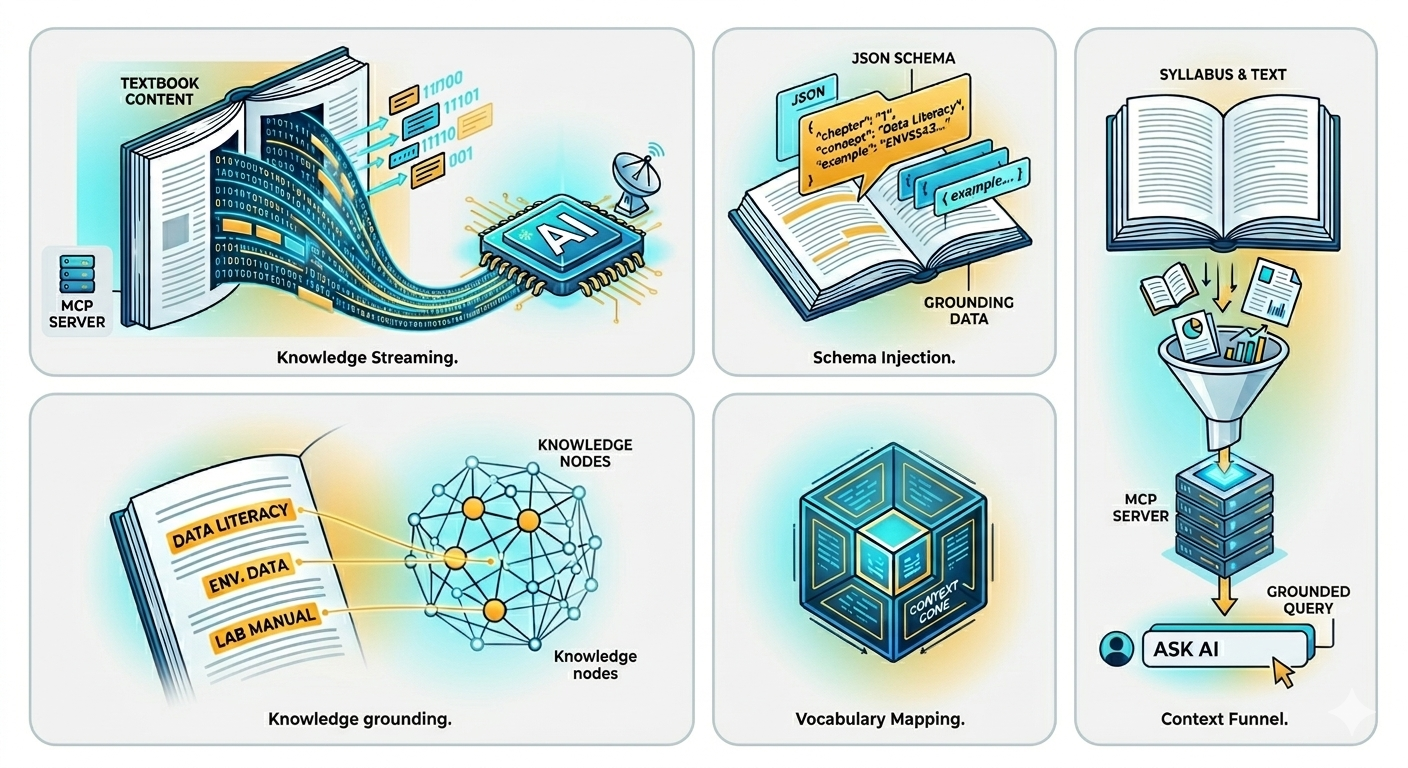
\includegraphics[keepaspectratio]{media/envsAI-TA.png}}

The auhor has designed a custom AI chat assistant based on this content.
We will be using the \href{https://positron.posit.co/}{Positron IDE} in
class, though it may be integrated into most common chat-based
interfaces. Ask your envsAI-TA a question, it can draw on the
vocabulary, context, and examples you are encountering here, in the
slides presented, and from the data we use in class, rather than giving
generic answers and AI slop. Think of it as giving your AI tutor a copy
of the syllabus, the textbook, and the lab manual, all at once.

Dr.~Dyer will provide a connection information and setup instructions on
the first day of class for
\href{https://bulletin.vcu.edu/search/?P=ENVS+543}{ENVS543:
Environmental Data Literacy}.

A PDF version of this book can be
\href{https://github.com/DyerlabTeaching/ENVS543-Book/releases/download/pdf_2025_12/Environmental-Data-Literacy.pdf}{downloaded
here}, though all the interactive content has been removed.

\section{License}\label{license}

© 2025 by Rodney J. Dyer.

All rights reserved. The author assumes no responsibility for the use or
misuse of information contained in this text. This book is licensed
under a \href{https://creativecommons.org/licenses/by-nc/4.0/}{Creative
Commons Attribution-NonCommercial 4.0 International License}.

You are free to:

\begin{itemize}
\tightlist
\item
  \emph{Share} --- copy and redistribute the material in any medium or
  format.\\
\item
  \emph{Adapt} --- remix, transform, and build upon the material.
\end{itemize}

Under the following terms:

\begin{itemize}
\tightlist
\item
  \emph{Attribution} --- You must give appropriate credit, provide a
  link to the license, and indicate if changes were made.\\
\item
  \emph{NonCommercial} --- You may not use the material for commercial
  purposes.
\end{itemize}

\section{How to Cite}\label{how-to-cite}

This is an open source, online textbook and can be cited as:

\begin{quote}
Dyer Rodney J. 2025. Environmental Data Literacy.
\url{https://environmentaldataliteracy.org}.
\end{quote}

Or use the following BibTeX entry.

\begin{Shaded}
\begin{Highlighting}[]
\VariableTok{@misc}\NormalTok{\{}\OtherTok{dyer\_2025}\NormalTok{,}
  \DataTypeTok{author}\NormalTok{ = \{Dyer, Rodney J\},}
  \DataTypeTok{title}\NormalTok{ = \{Environmental Data Literacy\},}
  \DataTypeTok{year}\NormalTok{ = \{2025\},}
  \DataTypeTok{url}\NormalTok{ = \{https://environmentaldataliteracy.org\}}
\NormalTok{\}}
\end{Highlighting}
\end{Shaded}

\section{Logistics}\label{logistics}

If you would like to compile this book yourself, you will find the
sourse code at its
\href{https://github.com/DyerlabTeaching/ENVS543-Book}{GitHub
repository}.

The following code runs each time you render the project. It will check
to see if you have all the required libraries, and if not, it installs
the needed ones and loads them into memory (so we do not get those
stupid package startup messages).

\begin{Shaded}
\begin{Highlighting}[]
\FunctionTok{source}\NormalTok{(}\StringTok{"package\_loader.R"}\NormalTok{)}

\NormalTok{libraries }\OtherTok{\textless{}{-}} \FunctionTok{extract\_libraries\_from\_markdown}\NormalTok{()}
\NormalTok{need\_to\_install }\OtherTok{\textless{}{-}} \FunctionTok{check\_missing\_packages}\NormalTok{( libraries )}
\FunctionTok{install\_missing\_packages}\NormalTok{( need\_to\_install )}
\ControlFlowTok{for}\NormalTok{( pkg }\ControlFlowTok{in}\NormalTok{ libraries ) \{ }
  \FunctionTok{suppressPackageStartupMessages}\NormalTok{( }
    \FunctionTok{library}\NormalTok{( pkg, }\AttributeTok{character.only =} \ConstantTok{TRUE}\NormalTok{) }
\NormalTok{  )}
\NormalTok{\}}
\NormalTok{ggplot2}\SpecialCharTok{::}\FunctionTok{theme\_set}\NormalTok{( }\FunctionTok{theme\_minimal}\NormalTok{( }\AttributeTok{base\_size=}\DecValTok{16}\NormalTok{) )}
\end{Highlighting}
\end{Shaded}

\section{Questions, Comments, or
Concerns}\label{questions-comments-or-concerns}

If you have any questions, comments or concerns regarding this material,
please contact \href{mailto://rjdyer@vcu.edu}{Dr.~Rodney Dyer}.
Additional teaching and reserach materials can also be found at
\href{https://rodneydyer.com}{rodneydyer.com}.

\bookmarksetup{startatroot}

\chapter*{Syllabus}\label{syllabus}
\addcontentsline{toc}{chapter}{Syllabus}

\markboth{Syllabus}{Syllabus}

\section*{ENVS 543: Environmental Data Literacy Fall
Semesters}\label{envs-543-environmental-data-literacy-fall-semesters}
\addcontentsline{toc}{section}{ENVS 543: Environmental Data Literacy
Fall Semesters}

\markright{ENVS 543: Environmental Data Literacy Fall Semesters}

\begin{quote}
Semester course; 3 lecture hours. 3 credits. Enrollment is restricted to
students with graduate standing or those with one course in statistics
and permission of the instructor. Develop quantitative skills for the
visualization, manipulation, analysis, and communication of
environmental ``big data.'' This course focuses on spatial environmental
data analysis, interpretation, and communication, using real-time data
from the Rice Rivers Center and the R statistical analysis environment.
\end{quote}

As both a student and instructor in statistics classes, I found I spent
a vast amount of time and effort describing the characteristics of
statistics (derivations, expectations, etc.). This is perfectly fine; it
is important on many levels to make sure that practitioners understand
the basis and context of all the kinds of analyses they use. However,
the drawback here, in my experience, is that once you've spent a
semester or year getting all this knowledge under your belt, and you can
easily demonstrate your understanding of the parameters in a model, you
cannot actually work with real data. This class is designed to produce
practitioners of data analysis.

\section*{Workflow in Data Analysis}\label{workflow-in-data-analysis}
\addcontentsline{toc}{section}{Workflow in Data Analysis}

\markright{Workflow in Data Analysis}

To understand data analytics, one needs to recognize the entire
workflow. Below is a brief graphical depiction of how analysis actually
works---in the real world. In this class, we will work on all of these
components using the open-source R language.

\begin{itemize}
\tightlist
\item
  \textbf{Collect:} Getting data from an external source into a format
  that you can use is often the most time-consuming step in the
  analysis. The content of this class will provide training in data
  import from local, online, and database sources.\\
\item
  \textbf{Visualize:} Visualizing data is key to understanding. In the
  image below, notice that the variables X and Y in all the displayed
  data sets have equivalent means, standard deviations, and correlation
  up to 2 decimal places! We will emphasize visualization, both static
  and dynamic, throughout this class.
\item
  \textbf{Transform:} Pulling data into your analysis ecosystem is not
  sufficient. Often the data need to be reformatted and reconfigured
  before it is actually usable.
\item
  \textbf{Model:} The application of models to subsets of data is often
  the step that takes the least amount of time and effort. However, the
  application of a model to data is not the endpoint. The model must be
  visualized and, many times, the underlying data or derivate data must
  be transformed and submitted to subsequent models.
\item
  \textbf{Communicate:} The effort we put into research and analyses is
  meaningless without effective communication of your data and findings
  to a broad audience. Here we will focus on how to develop effective
  data communication strategies and formats.
\end{itemize}

\section*{Learning Objectives}\label{learning-objectives}
\addcontentsline{toc}{section}{Learning Objectives}

\markright{Learning Objectives}

The purpose of this course is to help you build your data skills and to
develop a foundational understanding upon which subsequent courses will
build. The overarching goal here is to develop a working knowledge of
the R statistical computing language and enough proficiency to import
raw data and then iterate through the visualization, manipulation, and
analysis steps in the creation of output that is easily communicated to
a scientific audience.

The content of this course is built upon the following general Ctudent
Learning Objectives (CLO):

\subsection*{CLO 1: Use R to perform reproducible data analysis
workflows across environmental
contexts}\label{clo-1-use-r-to-perform-reproducible-data-analysis-workflows-across-environmental-contexts}
\addcontentsline{toc}{subsection}{CLO 1: Use R to perform reproducible
data analysis workflows across environmental contexts}

\begin{quote}
Students will demonstrate functional fluency in using R and its
associated libraries (e.g., Tidyverse, Quarto) for data import,
transformation, visualization, and analysis, establishing a
generalizable skillset for quantitative inquiry.
\end{quote}

\begin{itemize}
\tightlist
\item
  \emph{Bloom's Level:} Apply / Analyze.
\item
  \emph{Reinforces:} Seeing R as a tool for thinking and doing, not just
  syntax or statistical analysis.
\item
  \emph{Notes:} This aligns with the practical literacy needed to
  ``think with data'' in a coding environment. It emphasizes generalized
  fluency over memorization or syntax drills.
\end{itemize}

\subsection*{CLO 2: Analyze and interpret commonly encountered
environmental data and associated analyses using appropriate exploratory
and statistical
techniques}\label{clo-2-analyze-and-interpret-commonly-encountered-environmental-data-and-associated-analyses-using-appropriate-exploratory-and-statistical-techniques}
\addcontentsline{toc}{subsection}{CLO 2: Analyze and interpret commonly
encountered environmental data and associated analyses using appropriate
exploratory and statistical techniques}

\begin{quote}
Students will apply foundational exploratory and statistical approaches
(e.g., binomial models, contingency tables, regression, spatial
summaries) to common ecological, environmental, and evolutionary
datasets to support data-driven inference.
\end{quote}

\begin{itemize}
\tightlist
\item
  \emph{Bloom's Level:} Analyze / Evaluate.\\
\item
  \emph{Reinforces:} Judgment in data workflows, including exploratory
  iteration and critique.\\
\item
  \emph{Notes:} This keeps the emphasis on doing the analysis and
  interpreting results, not on statistical derivation of model
  components. It fits the framing: ``not a stats class'' but ``using
  common tools to make sense of real data.'' It also creates space for
  iteration and model refinement, aligning with the ``model, visualize,
  refine'' approach. +
\end{itemize}

\subsection*{CLO 3: Communicate data-driven findings using
publication-quality scientific writing and
visualizations.}\label{clo-3-communicate-data-driven-findings-using-publication-quality-scientific-writing-and-visualizations.}
\addcontentsline{toc}{subsection}{CLO 3: Communicate data-driven
findings using publication-quality scientific writing and
visualizations.}

\begin{quote}
Students will produce clear, compelling, and reproducible documents that
communicate quantitative findings, formatted according to scientific
norms and using tools like Quarto and Markdown.
\end{quote}

\begin{itemize}
\tightlist
\item
  \emph{Bloom's Level:} Create.\\
\item
  \emph{Reinforces:} Scientific communication and agile presentation of
  quantitative and qualitative information in industry-standard
  formats.\\
\item
  \emph{Notes:} This grounds communication in scientific practice, where
  students must compose and format their insights clearly and
  rigorously. It ties tightly into how you assess work (``as if
  submitting for publication'') and emphasizes narrative data fluency,
  not just procedural results.
\end{itemize}

\section*{Course Content \& Assessment}\label{course-content-assessment}
\addcontentsline{toc}{section}{Course Content \& Assessment}

\markright{Course Content \& Assessment}

This course is designed as a sequence of individual, stand-alone
modules. Each is self-contained and includes a lecture, slides, a larger
narrative document, a video demonstration, and an assessment.

\section*{Logistics}\label{logistics-1}
\addcontentsline{toc}{section}{Logistics}

\markright{Logistics}

\begin{itemize}
\tightlist
\item
  Course Instructor: Professor Rodney Dyer
\item
  Email: \href{mailto://rjdyer@vcu.edu}{rjdyer@vcu.edu}
\item
  Webpage: \href{https://rodneydyer.com}{rodneydyer.com}.
\end{itemize}

\section*{Required Materials}\label{required-materials}
\addcontentsline{toc}{section}{Required Materials}

\markright{Required Materials}

This course requires that you bring your own laptop or other computing
device that is capable of running RStudio and the R statistical
language. There is no required book and all content is provided via
online resources.

We will be using the \href{https://positron.posit.co/}{Positron IDE} to
write code, analysis, and narrative using markdown. We will also be
integrating the \textbf{envsAI-TA} chatbot interface for Positron, which
has been trained on \emph{all} course content and will serve as a
generic AI assistant for you in this course.

\section*{Assignments \& Grading
Policy}\label{assignments-grading-policy}
\addcontentsline{toc}{section}{Assignments \& Grading Policy}

\markright{Assignments \& Grading Policy}

The grade for this course is based upon the totality of the points
gained for all assignments, as well as a single large data analysis
project that will be due at the end of the semester. This final will
account for 10\% of your overall grade. Grades will be determined using
the normal 10\% scale:

\begin{itemize}
\tightlist
\item
  A (\textgreater= 90\%),\\
\item
  B (\textgreater= 80\% \& \textless{} 90\%),\\
\item
  C (\textgreater= 70\% \& \textless{} 80\%),
\item
  D (\textgreater= 60\% \& \textless{} 70\%), and
\item
  F (\textless{} 60\%).
\end{itemize}

All percentages are concrete, and scores will be rounded to the nearest
integer; no extra credit will be given.

\section*{Late Policy}\label{late-policy}
\addcontentsline{toc}{section}{Late Policy}

\markright{Late Policy}

All of the content in this class is given as take-home assignments and
tests. You will have a full 7 days to complete and turn in the work. The
intention here is to give you more than sufficient time to complete the
work because we do not rush data analysis. On the due date, I will post
the answers so you can check your work. After the answers are posted,
there will be no points awarded for late work.

\section*{Attendance Policy}\label{attendance-policy}
\addcontentsline{toc}{section}{Attendance Policy}

\markright{Attendance Policy}

All content is provided as slides, handouts, and video content. Much of
the work in this class will be conducted during the in-class session. As
such, you must show up to class if you intend to get the content. Data
analysis is a hands-on experience, and the more doing it you engage in
it, the more efficient you will become.

\section*{Disclaimer}\label{disclaimer}
\addcontentsline{toc}{section}{Disclaimer}

\markright{Disclaimer}

Note that the specifics of this Course Syllabus may be changed at any
time during the semester. You will be responsible for abiding by any
such changes that are communicated to you via email, course
announcement, and/or posting in the course discussion forums.

\section*{VCU Policies}\label{vcu-policies}
\addcontentsline{toc}{section}{VCU Policies}

\markright{VCU Policies}

Students should visit VCU's \href{http://go.vcu.edu/syllabus}{Syllabus
Information for Students} page and review all syllabus statement
information. The full university syllabus statement includes information
on safety, registration, the VCU Honor Code, student conduct,
withdrawal, and more.

Use \href{https://www.library.vcu.edu}{VCU Libraries} to find and access
library resources, spaces, technology, and services that support and
enhance all learning opportunities at the university.

\section*{Health and safety}\label{health-and-safety}
\addcontentsline{toc}{section}{Health and safety}

\markright{Health and safety}

\subsection*{Public health information}\label{public-health-information}
\addcontentsline{toc}{subsection}{Public health information}

Health advisories, including information about COVID-19 testing,
vaccination, supplies, and other public health measures, can be found at
the Safety and Risk Management website. Visit this site to stay informed
about recommendations for VCU and the surrounding communities.
Additional links to health, wellness, and safety information are on the
Life at VCU webpage.

\subsection*{Campus emergency
information}\label{campus-emergency-information}
\addcontentsline{toc}{subsection}{Campus emergency information}

Sign up to receive at VCU Alerts. It is essential to keep your
information up-to-date within VCU Alert and to keep your permanent
address and emergency contact information current in eServices. VCU uses
a variety of communication methods to alert the campus community about
emergencies and safety threats. Learn more about types of alerts online.
Know the emergency phone number for the VCU Police (828-1234), and
report suspicious activities and objects.

\subsection*{Managing stress}\label{managing-stress}
\addcontentsline{toc}{subsection}{Managing stress}

Students may experience situations or challenges that can interfere with
learning and interpersonal functioning, including stress, anxiety,
depression, alcohol and/or other drug use, concern for a friend or
family member, loss, sleep difficulties, feeling hopeless, or
relationship problems. There are numerous campus resources available to
students including University Counseling Services (804-828-6200 MPC
Campus, 804-828-3964 MCV Campus) which provides brief therapy treatment,
University Student Health Services (MPC 804 828-8828, MCV Campus 804
828-9220) and the Department of Recreation \& Well-Being (RecWell)
(804-828-9355). 24-hour emergency mental health support is available by
calling (804) 828-6200 or utilizing the National Suicide Prevention
Lifeline (dial 988).

\subsection*{Mandatory responsibility of faculty members to report
incidents of sexual
misconduct}\label{mandatory-responsibility-of-faculty-members-to-report-incidents-of-sexual-misconduct}
\addcontentsline{toc}{subsection}{Mandatory responsibility of faculty
members to report incidents of sexual misconduct}

All VCU faculty members are Responsible Employees as defined by
University policy. Responsible employees have a duty to report alleged
policy violations to the Title IX Coordinator. This includes incidents
of sexual harassment, sexual assault, dating \& domestic violence,
stalking, sexual exploitation, and related retaliation. Responsible
employees may report information through this form or by emailing
titleix@vcu.edu. For confidential support, contact University Counseling
Services, (804-828-6200 for MP Campus/804-828-3964 for MCV Campus) For
more information, visit our Title IX webpage.

\subsection*{Reading Days}\label{reading-days}
\addcontentsline{toc}{subsection}{Reading Days}

No classes or exams are held on Reading Day (Friday, Oct.~21, 2022)
except in instances where a student is involved in clinical and field
placements, practica, co-ops, internships, and other work-related
experiential learning activities. Faculty may not give an examination or
an assignment on those days. Instead, students are encouraged to use
these days for relaxation, study, and/or review of class materials.

\section*{Academic Success and
Integrity}\label{academic-success-and-integrity}
\addcontentsline{toc}{section}{Academic Success and Integrity}

\markright{Academic Success and Integrity}

\subsection*{Honor System: upholding academic
integrity}\label{honor-system-upholding-academic-integrity}
\addcontentsline{toc}{subsection}{Honor System: upholding academic
integrity}

The VCU Honor System policy describes the responsibilities of students,
faculty, and administration in upholding academic integrity. According
to this policy, ``Members of the academic community are required to
conduct themselves in accordance with the highest standards of academic
honesty, ethics, and integrity at all times.'' Students are expected to
read the policy in full and learn about requirements.

\subsection*{Early academic alerts}\label{early-academic-alerts}
\addcontentsline{toc}{subsection}{Early academic alerts}

VCU's Early Notification Program supports student success. If, as an
instructor, I am concerned about your academic engagement or performance
in the first few weeks of class, you may receive a Progress Report email
encouraging you to reach out to me after class or during student hours
(office hours) for additional support. As a community of care, your
academic advisor, the Writing Center, and the Campus Learning Center may
also follow up to provide additional layers of support.

\subsection*{Students with
disabilities}\label{students-with-disabilities}
\addcontentsline{toc}{subsection}{Students with disabilities}

VCU is committed to ensuring that all students maintain equal access to
all aspects of the university, including educational experiences through
the provision of reasonable accommodations and academic adjustments. In
addition to being a requirement under Section 504 of the Rehabilitation
Act of 1973 and the Americans with Disabilities Act, this speaks
directly to VCU's mission of inclusion, equity, and access. To receive
accommodations or other disability-related supports, students must
register with the Office of Student Accessibility and Educational
Opportunity on the Monroe Park Campus (828-2253) or the Division for
Academic Success on the MCV campus (828-9782). Students and faculty can
visit the Student Accessibility and Educational Opportunity website
and/or the Division for Academic Success website for additional
information. Once students have completed the registration process, they
will be provided with a letter of accommodation. They should provide a
copy to their instructor(s) and attempt to schedule a meeting to discuss
the implementation of accommodations as early in the semester as
possible.

\subsection*{Career Services}\label{career-services}
\addcontentsline{toc}{subsection}{Career Services}

Looking for ways to tie what you are learning in your class to your
future career or professional goals? VCU Career Services provides career
planning services for all current VCU students and alumni. Career
Services can help students with finding a work-study job on/off campus,
resume writing, internship development, interviewing, preparing for
graduate school, networking, or job searching. Students are invited to
attend career events and workshops and schedule individualized career
advising appointments.

\section*{Registration, Attendance, and Financial
Responsibilities}\label{registration-attendance-and-financial-responsibilities}
\addcontentsline{toc}{section}{Registration, Attendance, and Financial
Responsibilities}

\markright{Registration, Attendance, and Financial Responsibilities}

\subsection*{Class registration is required for
attendance}\label{class-registration-is-required-for-attendance}
\addcontentsline{toc}{subsection}{Class registration is required for
attendance}

Students may attend only those classes for which they have registered.
Faculty may not add students to class rosters. If students are attending
a class for which they have not registered, they must stop attending.

\subsection*{Attendance and consequences of poor
attendance}\label{attendance-and-consequences-of-poor-attendance}
\addcontentsline{toc}{subsection}{Attendance and consequences of poor
attendance}

The instructional programs at VCU are based upon a series of class
meetings involving lectures, discussions, field experiences, special
readings, and reporting assignments. Therefore, it is important for each
student to be in attendance regularly. A student who misses a class
session is responsible for completing all material covered or
assignments made during the absence.

\begin{itemize}
\item
  Students having attendance problems should contact their instructor to
  explain the reasons for nonattendance and to discuss the feasibility
  of continuing in the course. If the student has fallen so far behind
  that the successful completion of the course is impossible, the
  student should withdraw from the course before the end of the first 10
  weeks of classes (by Oct.~28, 2022).
\item
  If the student continues to miss class and does not officially
  withdraw from the course, the instructor may withdraw the student for
  nonattendance with a mark of ``W'\,' before the end of the first 10
  weeks of classes or may assign an academic grade at the end.
  Withdrawals are not permitted after the end of the first 10 weeks of
  classes. For classes that do not conform to the semester calendar, the
  final withdrawal date occurs when half of the course has been
  completed.
\end{itemize}

\subsection*{Withdrawal from classes}\label{withdrawal-from-classes}
\addcontentsline{toc}{subsection}{Withdrawal from classes}

Before withdrawing from classes, students should consult their
instructor as well as other appropriate university offices. Withdrawing
from classes may negatively impact a student's financial aid award and
his or her semester charges. To discuss financial aid and the student
bill, contact the Student Financial Management Center (RAMQ) regarding
the impact on your financial aid.

\subsection*{Military short-term training or
deployment}\label{military-short-term-training-or-deployment}
\addcontentsline{toc}{subsection}{Military short-term training or
deployment}

If military students receive orders for short-term training or for
deployment/mobilization, they should inform and present their orders to
Military Student Services and to their professor(s). For further
information on policies and procedures, contact Military Student
Services at 828-5993.

\subsection*{Students representing the university -- excused
absences}\label{students-representing-the-university-excused-absences}
\addcontentsline{toc}{subsection}{Students representing the university
-- excused absences}

Students who represent the university (athletes and others) do not
choose their schedules. All student-athletes should provide their
schedules to their instructors at the beginning of the semester. The
Intercollegiate Athletic Council strongly encourages faculty to treat
missed classes or exams (because of a scheduling conflict) as excused
absences and urges faculty to work with the students to make up the work
or exam.

\subsection*{Student financial
responsibility}\label{student-financial-responsibility}
\addcontentsline{toc}{subsection}{Student financial responsibility}

Students assume the responsibility of full payment of tuition and fees
generated from their registration, all charges for housing and dining
services, and other applicable miscellaneous charges. Students are
ultimately responsible for any unpaid balance on their account as a
result of the University Financial Aid Office or their third-party
sponsor canceling or reducing their award(s).

\section*{Technology}\label{technology}
\addcontentsline{toc}{section}{Technology}

\markright{Technology}

\subsection*{Computer and network use}\label{computer-and-network-use}
\addcontentsline{toc}{subsection}{Computer and network use}

All students are expected to know and comply with VCU's Computer and
Network Use policy.

\subsection*{Student email standard}\label{student-email-standard}
\addcontentsline{toc}{subsection}{Student email standard}

Email is considered an official method of communication at VCU. Students
are expected to check their official VCU email on a frequent and
consistent basis (the university recommends daily) in order to remain
informed of university-related communications. Students are responsible
for the consequences of not reading, in a timely fashion,
university-related communications sent to their official VCU student
email account. Mail sent to the VCU email address may include
notification of university-related actions, including disciplinary
action. Students must read this standard in its entirety.

\subsection*{Faculty communication with
students}\label{faculty-communication-with-students}
\addcontentsline{toc}{subsection}{Faculty communication with students}

VCU instructional faculty, administrators, and staff maintain
confidentiality of student records and disclose information in
accordance with the Family Educational Rights and Privacy Act (FERPA).
This means that VCU officials may disclose student record information
without the consent of the student in certain situations. To support
university operations, for example, VCU officials share information
about students with other educational officials as necessary to perform
their job duties. FERPA permits this disclosure to school officials who
have a legitimate educational interest in the student information. In
addition, VCU officials have obligations to report information shared by
a student depending on the content of that information, for example, in
compliance with VCU's policy on the duty to report. Unless FERPA permits
a certain disclosure, VCU generally requires consent from a student to
disclose information from their education record to another individual.
You may find additional information on the VCU FERPA website.

\section*{Important dates}\label{important-dates}
\addcontentsline{toc}{section}{Important dates}

\markright{Important dates}

Important dates for the current and future semesters are listed in the
VCU Academic Calendar.

\emph{Let's start!}

\part{R Fundamentals}

This section contains chapters covering basic \texttt{R} and data
manipulation skills.

\chapter{Markdown}\label{markdown}

\pandocbounded{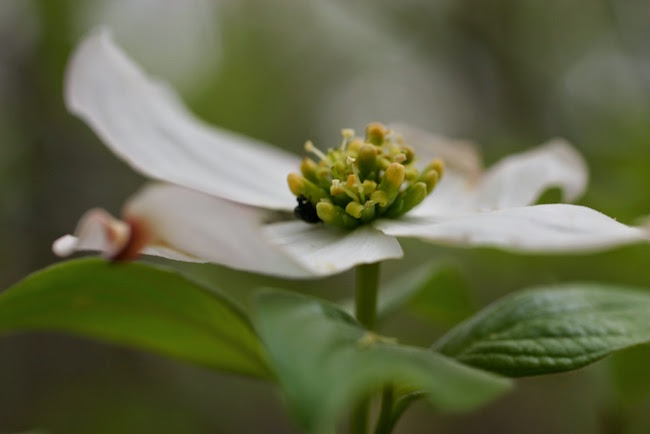
\includegraphics[keepaspectratio]{media/chapter_markdown.jpg}}

\begin{quote}
Markdown \& Notebooks provide interactive documents for more effective
data communication
\end{quote}

\section{Lecture Materials}\label{lecture-materials}

\begin{quote}
\textbf{Lecture Slides:} Available interactively in the
\href{https://dyerlabteaching.github.io/Markdown/slides.html\#/title-slide}{online
version}
\end{quote}

\begin{figure}[H]

{\centering \pandocbounded{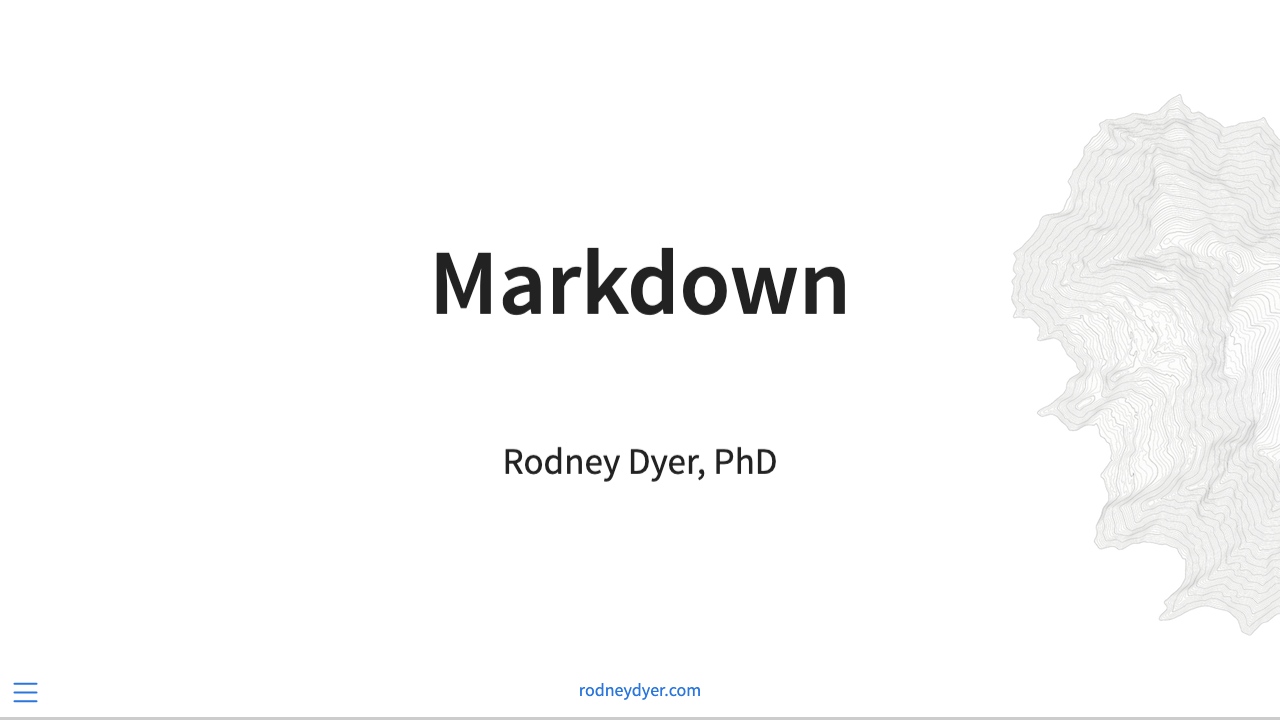
\includegraphics[keepaspectratio]{media/slides_markdown.png}}

}

\caption{Lecture Slides}

\end{figure}%

\section{Impetus}\label{impetus}

In current data analytics and communication, there are a wide variety of
platforms on which we can provide summaries and insights regarding our
work. Each of these end points requires a non-insignificant amount of
effort to learn these systems. Moreover, they all are \emph{cul de sacs}
in that all the effort you exert to learn one will not allow you to get
the benefits of any other platform than the one you just learned.

\begin{quote}
This is stupid. - R. Dyer
\end{quote}

Enter \href{https://pandoc.org}{Pandoc}, the universal document
converter. Some really smart programmers have put together a set of
software that allows you to convert from or two (and hence between)
different document types given that most documents are regularly
structured. With Pandoc, it does not matter if you do or do not have
Word or PowerPoint or EPub or LaTeX or whatever, as long as you can
create one of the supported types, you can convert that input into a
huge variety of output types.

\section{Pandoc Supported
Conversions}\label{pandoc-supported-conversions}

\begin{figure}[H]

{\centering \pandocbounded{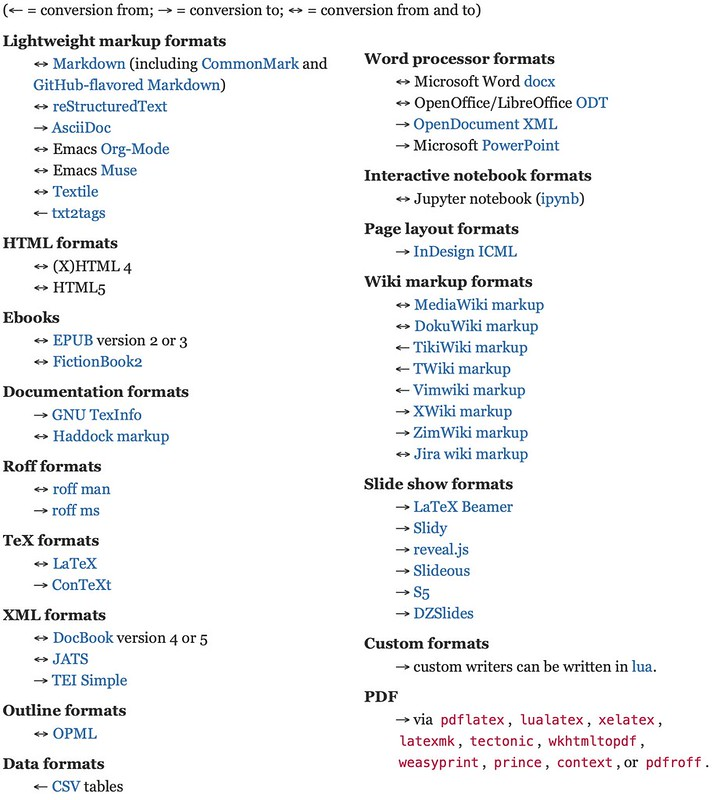
\includegraphics[keepaspectratio]{media/conversion_formats.jpg}}

}

\caption{Conversion Formats}

\end{figure}%

This is critical for us because Code is just text. Once it is evaluated,
it can replaced with:

\begin{itemize}
\tightlist
\item
  Numerical values from one or more calculations,
\item
  Textual content from analyses or manipulation, or
\item
  Graphical content from plots.
\end{itemize}

As such, we can embed R code within raw text to create our analyses and
documents.

\section{Installing Quarto for
Markdown}\label{installing-quarto-for-markdown}

The first step is to go to \href{https://quarto.org}{quarto} and
download the quarto engine for your particular laptop.

\section{Markdown Syntax}\label{markdown-syntax}

For maximum usability, the document that we embed our code into should
be as widely available as possible---unhindered by the necessity of
having a particular program just to view the content. For this, R uses
\href{https://en.wikipedia.org/wiki/Markdown}{Markdown}, created by John
Gruber \& Aaron Swartz in 2004. Markdown was created so that people are
enabled ``\ldots to write using an easy-to-read and easy-to-write plain
text format\ldots{}''

Because everything is text, it is easy share and collaborate using
Markdown, and for R, it is how we can make a wide array of output
document types including (but not limited to):

\begin{itemize}
\tightlist
\item
  Conventional documents (PDF, Word, RTF, etc.)
\item
  HTML pages with interactive elements (this document here is an
  interactive html document).
\item
  Presentations (LaTeX, PowerPoint, JavaScript, etc.)
\item
  Dashboards with interactive content.
\end{itemize}

\section{Text Markup}\label{text-markup}

When we make a document, presentation, or any other output, there are
only a finite set of different text components we can put into the
document. The document itself does not need to be heavy or bloated, it
is just text (though surprisingly, a blank Word document on my laptop
with nothing in the document itself is still 12KB in size!). Common
elements include:

\begin{itemize}
\tightlist
\item
  Headers \& Titles
\item
  Typography such as italic, bold, underline, strike through
\item
  Lists (numbered or as bullets)
\item
  Pictures and links
\item
  Page numbers, tables of contents, etc.
\end{itemize}

What Markdown does is allows you to type these components and use
`marking' around the elements to make them different from regular text.
It is really, amazingly simple.

Title and headers are created by prepending a hashtag

\# Header 1\\
\#\# Header 2\\
\#\#\# Header 3\\
\#\#\#\# Header 4

are knit into the proper header styles.

The actual appearance of the headers are determined by where it is being
presented (e.g., in Word it will take the default typography and font
attributes, etc.).

In text markdown examples are shown below and are contained within
paragraphs of text. Individual paragraphs are delimited by either a
blank line between them or two spaces at the end of the sentence.

{\def\LTcaptype{none} % do not increment counter
\begin{longtable}[]{@{}ll@{}}
\toprule\noalign{}
Markdown & Rendered As \\
\midrule\noalign{}
\endhead
\bottomrule\noalign{}
\endlastfoot
plain text & plain text \\
*italic* & \emph{italic} \\
**bold** & \textbf{bold} \\
\textasciitilde\textasciitilde strike
through\textasciitilde\textasciitilde{} & \st{strike through} \\
\end{longtable}
}

You can also embed links and images. Both of these are configured in two
parts. For links, you need to specify the text that can be clicked upon
and it \emph{must} be surrounded in \emph{square brackets}. The link to
the web or file or image is right next to the square brackets and is
contained within \emph{parentheses}. The difference between link and
image is that images have alternative text (or at times captions) and
the whole thing has an exclamation mark in front of it. Here are some
examples.

{\def\LTcaptype{none} % do not increment counter
\begin{longtable}[]{@{}
  >{\raggedright\arraybackslash}p{(\linewidth - 2\tabcolsep) * \real{0.4861}}
  >{\raggedright\arraybackslash}p{(\linewidth - 2\tabcolsep) * \real{0.5139}}@{}}
\toprule\noalign{}
\begin{minipage}[b]{\linewidth}\raggedright
Markdown
\end{minipage} & \begin{minipage}[b]{\linewidth}\raggedright
Rendered As
\end{minipage} \\
\midrule\noalign{}
\endhead
\bottomrule\noalign{}
\endlastfoot
{[}SLSS{]}(https://slss.vcu.edu) & \href{https://slss.vcu.edu}{SLSS} \\
!{[}Goat{]}(media/goat.jpg) &
\pandocbounded{
\includegraphics[keepaspectratio,alt={alt text}]{media/goat.jpg}} \\
\end{longtable}
}

Lists (both numbered and unordered) are created using dashes or
asterisks.

\begin{itemize}
\tightlist
\item
  Bullet 1\\
\item
  Bullet 2\\
\item
  Bullet 3
\end{itemize}

Will be turned into an unordered list as:

\begin{itemize}
\tightlist
\item
  Bullet 1\\
\item
  Bullet 2\\
\item
  Bullet 3
\end{itemize}

Whereas the following raw text.\footnote{Pielou EC, (1984) The
  interpretation of ecological data: A primer on classification and
  ordination. 288pg. ISBN:
  \href{https://www.wiley.com/en-us/The+Interpretation+of+Ecological+Data\%3A+A+Primer+on+Classification+and+Ordination-p-9780471889502}{978-0-471-88950-2}}

1. First\\
1. Second\\
1. Third

Will be rendered in list format as:

\begin{enumerate}
\def\labelenumi{\arabic{enumi}.}
\tightlist
\item
  First\\
\item
  Second\\
\item
  Third
\end{enumerate}

Actually, you \emph{can} just use \texttt{1.} in front of every line if
you like, it will auto-number them for you when it makes a list. I tend
to do this because it makes it a bit easier in case I want to reorder
the list later and I don't have to go back and change the numbers.

\section{Code \& Text}\label{code-text}

On of the strengths of RMarkdown is the ability to mix code and text
together in one place. This allows us to bring all of our analyses
\emph{and} data as close to one another as possible, helping with
reproducibility and error reduction.

\subsection{Inline Code}\label{inline-code}

You can easily integrate code, into the text, either to be displayed
\emph{OR} to be evaluated. For example, in \texttt{R} you get the value
of \(\pi\) by the constant \texttt{pi}. Type that into the console and
it will return 3.1415927.

If you look at the RMarkdown for that paragraph above, it looks like the
following before knitting:

\begin{Shaded}
\begin{Highlighting}[]
\NormalTok{You can easily integrate code, into the text, either to be displayed }\SpecialCharTok{*}\NormalTok{OR}\SpecialCharTok{*}\NormalTok{ to be evaluated.  For example, }\ControlFlowTok{in} \StringTok{\textasciigrave{}}\AttributeTok{R}\StringTok{\textasciigrave{}}\NormalTok{ you get the value of }\SpecialCharTok{$}\NormalTok{\textbackslash{}pi}\SpecialCharTok{$}\NormalTok{ by the constant }\StringTok{\textasciigrave{}}\AttributeTok{pi}\StringTok{\textasciigrave{}}\NormalTok{. Type that into the console and it will return }\DecValTok{3}\NormalTok{.}\FloatTok{1415927.}
\end{Highlighting}
\end{Shaded}

Notice the following parts:

\begin{itemize}
\tightlist
\item
  Symbols: The \(\pi\) symbol is created by the name of the symbol
  surrounded by dollar signs. \$~\pi \$. There are a ton of symbols and
  equations you can use, all borrowed from LaTeX, so if you need
  complicated equations or symbols, this is not a problem.
\item
  Text rendered as code (in typography) but not evaluated: Both the `R`
  and the `pi` are examples here. Nothing is evaluated, but it
  \emph{looks} like code.
\item
  Evaluated R Code: Any code between
  \texttt{\textbackslash{}}r\texttt{and}`\texttt{will\ be\ evaluated\ as\ R\ code\ within\ the\ text.\ When\ you\ knit\ the\ document,\ it\ will\ be\ run\ and\ the\ contents\ between\ the}`r\texttt{and}`\texttt{are\ replaced\ by\ the\ output\ of\ the}R\texttt{code.\ The\ example\ here\ was\ \textbackslash{}}pi`
  at the end of the last sentence.
\end{itemize}

\subsection{Code Chunks}\label{code-chunks}

In addition to code within the text, RMarkdown supports \emph{code
chunks}, which can be one or many lines of raw \texttt{R} code. This
code is executed and the results are merged into the markdown in the
document (text, graphical, interactive widgets, whatever) before
knitting.

Each chunk is enclosed within boundary rows, the top row \textbf{must}
contain three acute accents (back ticks - `) followed by the letter r in
curly brackets ```\{r\}. The end of the chunk is indicated by three back
ticks on their own line such as ```. Everything between these two
enclosing lines is treated as \texttt{R} code and is subject to
evaluation when you re-knit the document.

Here is what a chunk looks like in markdown that prints out a simple
message ``This is text from a chunk.

```\{r\}\\
print(``This is text from a chunk'')\\
```

When it is evaluated, the \texttt{R} interpreter removes the first and
last rows, and executes the code within them. By default, the code is
presented as a box in the output as well as any output that is produced
from the code.

\begin{Shaded}
\begin{Highlighting}[]
\FunctionTok{print}\NormalTok{(}\StringTok{"This is text from a chunk"}\NormalTok{)}
\end{Highlighting}
\end{Shaded}

\begin{verbatim}
[1] "This is text from a chunk"
\end{verbatim}

The first line in the chunk can also be used to modify the behavior of
the code. There are several options that you can place within the curly
brackets, including:

\begin{itemize}
\tightlist
\item
  \texttt{\{r\ eval=FALSE\}}: Will not evaluate (e.g., run) the code.
  The default value is \texttt{TRUE}.\\
\item
  \texttt{\{r\ echo=FALSE\}}: Will not show the code in the document.
  This is great for our final version of our analyses, we want the
  output but not the code chunks showing. The default value is
  \texttt{TRUE}.\\
\item
  \texttt{\{r\ message=FALSE,\ warning=FALSE,\ error=FALSE\}}: These
  suppress the messages that \texttt{R} prints out on occasion.
\end{itemize}

See the reference guide for several more options you can put into the
header of each chunk.

\section{Code Chunks in Document}\label{code-chunks-in-document}

There are some very \emph{fundamental} issues regarding chunks, the
\texttt{R} environment, and documents that should be pointed out here.

\begin{enumerate}
\def\labelenumi{\arabic{enumi}.}
\tightlist
\item
  The \texttt{R} environment (see tab labeled \textbf{Environment} in
  the RStudio interface) has all the variables and new functions that
  you have created listed and available for use.
\item
  An \texttt{R} Markdown document is not a `living' environment. If you
  make a change in a chunk, you \emph{must} rerun that chunk to have the
  output available and inserted into the \textbf{Environment}. It does
  not do it automagically.
\item
  When you knit a document, the \textbf{only} data it has is what is
  actually in the document itself. It does not look to the general
  \textbf{Environment} for variables and functions. This means that if
  you create a variable or load data using the Console and then
  reference it in the Document, it will fail when you try to knit the
  document.
\item
  All the code and variables in a document (if they are not within a
  chunk with \texttt{eval=FALSE}) is visible to everything in the
  document below where it was defined.\\
\item
  Chunks are evaluated from the top of the document to the bottom of the
  document.\\
\item
  The options for each chunk are available from the setup menu on the
  top right of the chunk itself (the gear icon). Additional options
  include a button to run all the chunks prior to this one as well as
  running this particular chunk (see image).
\end{enumerate}

\begin{figure}[H]

{\centering \pandocbounded{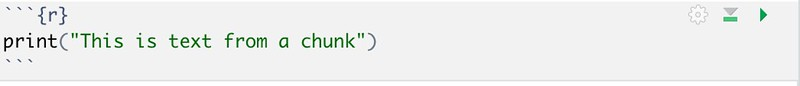
\includegraphics[keepaspectratio]{media/chunk_options.jpg}}

}

\caption{Option buttons for each chunk include a quick menu for optoins
(gear), the ability to run all the chunks above this one (triangle and
line button in the middle), and run this particular chunk (play
button).}

\end{figure}%

\chapter{Data Types}\label{data-types}

\pandocbounded{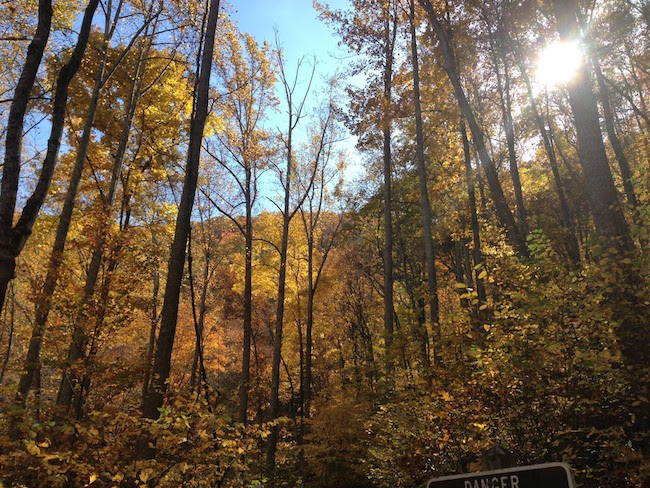
\includegraphics[keepaspectratio]{media/chapter_datatypes.jpg}}

\begin{quote}
When we work with an analysis language, we need to be very precise about
how we represent the data we collect. R is a general analysis language
and has a wide range of native data types and can easily be expanded
using the package system.
\end{quote}

\section{Lecture Materials}\label{lecture-materials-1}

\begin{quote}
\textbf{Lecture Slides:} Available interactively in the
\href{https://dyerlabteaching.github.io/Basic-Data-Types/slides.html\#/title-slide}{online
version}
\end{quote}

\begin{figure}[H]

{\centering \pandocbounded{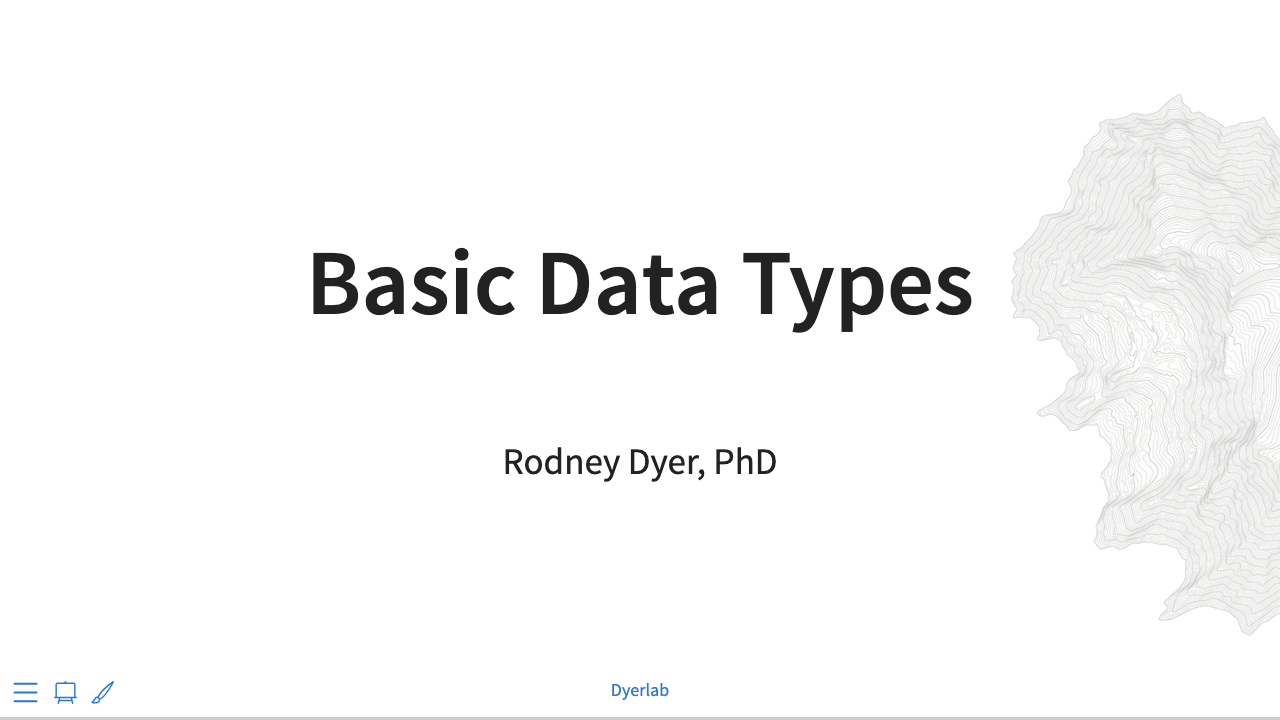
\includegraphics[keepaspectratio]{media/slides_datatypes.png}}

}

\caption{Lecture Slides}

\end{figure}%

\section{Missing Data}\label{missing-data}

\begin{quote}
The Absence of Data
\end{quote}

The most fundamental type of data in \texttt{R} is data that does not
exist! Missing data! It is represented as \texttt{NA}

\begin{Shaded}
\begin{Highlighting}[]
\NormalTok{x }\OtherTok{\textless{}{-}} \ConstantTok{NA}
\end{Highlighting}
\end{Shaded}

\section{Numerical Data}\label{numerical-data}

\begin{quote}
Numerical data contains all numerical represenations.
\end{quote}

By far, the most common kind of data we use in our analyses is numerical
data. This may represent measured things like \texttt{height},
\texttt{snout-vent\ length} (whatever that is), \texttt{depth},
\texttt{age}, etc. In data analysis, we commonly take (or obtain)
measurements from several items and then try to characterize them using
summaries and visualization.

In \texttt{R}, the numerical data type can be defined as:

\begin{Shaded}
\begin{Highlighting}[]
\NormalTok{X }\OtherTok{\textless{}{-}} \DecValTok{42}
\end{Highlighting}
\end{Shaded}

Notice how the numerical value of \texttt{42} is assigned to the
variable named \texttt{X}. To have \texttt{R} print out the value of a
particular variable, you can type its name in the console and it will
give it to you.

\begin{Shaded}
\begin{Highlighting}[]
\NormalTok{X}
\end{Highlighting}
\end{Shaded}

\begin{verbatim}
[1] 42
\end{verbatim}

\subsection{Operators}\label{operators}

Numeric types have a ton of normal operators that can be used. Some
examples include:

The usual \emph{arithmetic operators}:

\begin{Shaded}
\begin{Highlighting}[]
\NormalTok{x }\OtherTok{\textless{}{-}} \DecValTok{10}
\NormalTok{y }\OtherTok{\textless{}{-}} \DecValTok{23}

\NormalTok{x }\SpecialCharTok{+}\NormalTok{ y}
\end{Highlighting}
\end{Shaded}

\begin{verbatim}
[1] 33
\end{verbatim}

\begin{Shaded}
\begin{Highlighting}[]
\NormalTok{x }\SpecialCharTok{{-}}\NormalTok{ y}
\end{Highlighting}
\end{Shaded}

\begin{verbatim}
[1] -13
\end{verbatim}

\begin{Shaded}
\begin{Highlighting}[]
\NormalTok{x }\SpecialCharTok{*}\NormalTok{ y}
\end{Highlighting}
\end{Shaded}

\begin{verbatim}
[1] 230
\end{verbatim}

\begin{Shaded}
\begin{Highlighting}[]
\NormalTok{x }\SpecialCharTok{/}\NormalTok{ y}
\end{Highlighting}
\end{Shaded}

\begin{verbatim}
[1] 0.4347826
\end{verbatim}

You have the \emph{exponential}:

\begin{Shaded}
\begin{Highlighting}[]
\DocumentationTok{\#\# x raised to the y}
\NormalTok{x}\SpecialCharTok{\^{}}\NormalTok{y}
\end{Highlighting}
\end{Shaded}

\begin{verbatim}
[1] 1e+23
\end{verbatim}

\begin{Shaded}
\begin{Highlighting}[]
\DocumentationTok{\#\# the inverse of an exponent is a root, here is the 23rd root of 10}
\NormalTok{x}\SpecialCharTok{\^{}}\NormalTok{(}\DecValTok{1}\SpecialCharTok{/}\NormalTok{y)}
\end{Highlighting}
\end{Shaded}

\begin{verbatim}
[1] 1.105295
\end{verbatim}

The \emph{logarithmic}:

\begin{Shaded}
\begin{Highlighting}[]
\DocumentationTok{\#\# the natural log}
\FunctionTok{log}\NormalTok{(x)}
\end{Highlighting}
\end{Shaded}

\begin{verbatim}
[1] 2.302585
\end{verbatim}

\begin{Shaded}
\begin{Highlighting}[]
\DocumentationTok{\#\# Base 10 log}
\FunctionTok{log}\NormalTok{(x,}\AttributeTok{base=}\DecValTok{10}\NormalTok{)}
\end{Highlighting}
\end{Shaded}

\begin{verbatim}
[1] 1
\end{verbatim}

And the \emph{modulus operator}:

\begin{Shaded}
\begin{Highlighting}[]
\NormalTok{y }\SpecialCharTok{\%\%}\NormalTok{ x}
\end{Highlighting}
\end{Shaded}

\begin{verbatim}
[1] 3
\end{verbatim}

If you didn't know what this one is, don't worry. The modulus is just
the \emph{remainder after division} like you did in grade school. The
above code means that \emph{23 divided by 10 has a remainder of 3}. I
include it here just to highlight the fact that many of the operators
that we will be working with in \texttt{R} are created by more than just
a single symbol residing at the top row of your computer keyboard. There
are just too few symbos on the normal keyboard to represent the breath
of operators. The authors of \texttt{R} have decided that using
combinations of symbols to handle these and you will get used to them in
not time at all.

\subsection{Introspection \& Coercion}\label{introspection-coercion}

The \texttt{class()} of a numeric type is (wait for it)\ldots{}
\texttt{numeric} (those \texttt{R} programmers are sure clever).

\begin{Shaded}
\begin{Highlighting}[]
\FunctionTok{class}\NormalTok{( }\DecValTok{42}\NormalTok{ )}
\end{Highlighting}
\end{Shaded}

\begin{verbatim}
[1] "numeric"
\end{verbatim}

In this case \texttt{class} is the name of the function and there are
one or more things we pass to that function. These \textbf{must} be
enclosed in the parenthesis associated with \texttt{class}. The
parantheses \textbf{must} be \emph{right next to} the name of the
function. If you put a space betwen the word \texttt{class} and the
parentheses, it may not work the way you would like it to. You've been
warned.

The stuff inside the parenthesis are called \emph{arguments} and are the
data that we pass to the function itself. In this case we pass a value
or varible to the \texttt{class} function and it does its magic and
tells us what kind of data type it is. Many functions have several
arguements that can be passed to them, some optional, some not. We will
get more into that on the lecture covering
\href{https://dyerlab.github.io/ENVS-Lectures/functions/slides.html}{Functions}.

It is also possible to inquire if a particular variable is of a certain
class. This is done by using the \texttt{is.*} set of functions.

\begin{Shaded}
\begin{Highlighting}[]
\FunctionTok{is.numeric}\NormalTok{( }\DecValTok{42}\NormalTok{ )}
\end{Highlighting}
\end{Shaded}

\begin{verbatim}
[1] TRUE
\end{verbatim}

\begin{Shaded}
\begin{Highlighting}[]
\FunctionTok{is.numeric}\NormalTok{( }\StringTok{"dr dyer"}\NormalTok{ )}
\end{Highlighting}
\end{Shaded}

\begin{verbatim}
[1] FALSE
\end{verbatim}

Sometimes we may need to turn one kind of class into another kind.
Consider the following:

\begin{Shaded}
\begin{Highlighting}[]
\NormalTok{x }\OtherTok{\textless{}{-}} \StringTok{"42"}
\FunctionTok{is.numeric}\NormalTok{( x )}
\end{Highlighting}
\end{Shaded}

\begin{verbatim}
[1] FALSE
\end{verbatim}

\begin{Shaded}
\begin{Highlighting}[]
\FunctionTok{class}\NormalTok{(x)}
\end{Highlighting}
\end{Shaded}

\begin{verbatim}
[1] "character"
\end{verbatim}

It is a \texttt{character} data type because it is enclosed within a set
of quotes. However, we can \emph{coerce} it into a numeric type by:

\begin{Shaded}
\begin{Highlighting}[]
\NormalTok{y }\OtherTok{\textless{}{-}} \FunctionTok{as.numeric}\NormalTok{( x )}
\FunctionTok{is.numeric}\NormalTok{( y )}
\end{Highlighting}
\end{Shaded}

\begin{verbatim}
[1] TRUE
\end{verbatim}

\begin{Shaded}
\begin{Highlighting}[]
\NormalTok{y}
\end{Highlighting}
\end{Shaded}

\begin{verbatim}
[1] 42
\end{verbatim}

\section{Character Data}\label{character-data}

\begin{quote}
Character data represents textual content.
\end{quote}

The data type \texttt{character} is intended to represent textual data
such as \emph{actual texts}, names of objects, and other contnet that is
intended to help both you and the audience you are trying to reach
better understand your data.

\begin{Shaded}
\begin{Highlighting}[]
\NormalTok{name }\OtherTok{\textless{}{-}} \StringTok{"Dyer"}
\NormalTok{sport }\OtherTok{\textless{}{-}} \StringTok{"Frolf"}
\end{Highlighting}
\end{Shaded}

The two variables above have a sequence of characters enclosed by a
double quote. You can use a single quote instead, \emph{however} the
enclosing quoting characters must be the same (e.g., you cannot start
with a single quote and end with a double).

\subsection{Lengths}\label{lengths}

The length of a string is a measure of how many varibles there are, not
the number of characters within it. For example, the length of
\texttt{dyer} is

\begin{Shaded}
\begin{Highlighting}[]
\FunctionTok{length}\NormalTok{(name)}
\end{Highlighting}
\end{Shaded}

\begin{verbatim}
[1] 1
\end{verbatim}

because it only has one character but the number of characters within it
is:

\begin{Shaded}
\begin{Highlighting}[]
\FunctionTok{nchar}\NormalTok{(name)}
\end{Highlighting}
\end{Shaded}

\begin{verbatim}
[1] 4
\end{verbatim}

Length is defined specifically on the number of elements in a vector,
and technically the variable \texttt{dyer} is a vector of length one. If
we concatinate them into a vector (go see the vector content)

\begin{Shaded}
\begin{Highlighting}[]
\NormalTok{phrase }\OtherTok{\textless{}{-}} \FunctionTok{c}\NormalTok{( name, sport )}
\end{Highlighting}
\end{Shaded}

we find that it has a length of 2

\begin{Shaded}
\begin{Highlighting}[]
\FunctionTok{length}\NormalTok{(phrase)}
\end{Highlighting}
\end{Shaded}

\begin{verbatim}
[1] 2
\end{verbatim}

And if we ask the vector how many characters are in the elements it
contains, it gives us a vector of numeric types representing the number
of letters in each of the elements.

\begin{Shaded}
\begin{Highlighting}[]
\FunctionTok{nchar}\NormalTok{(phrase)}
\end{Highlighting}
\end{Shaded}

\begin{verbatim}
[1] 4 5
\end{verbatim}

\subsection{Putting Character Objects
Together}\label{putting-character-objects-together}

The binary \texttt{+} operator has not been defined for objects of class
\texttt{character}, which is understandable once we consider all the
different ways we may want to put the values contained in the variables
together. If you try it, \texttt{R} will complain.

\begin{Shaded}
\begin{Highlighting}[]
\NormalTok{name }\SpecialCharTok{+}\NormalTok{ sport}
\end{Highlighting}
\end{Shaded}

\begin{verbatim}
Error in `name + sport`:
! non-numeric argument to binary operator
\end{verbatim}

The \texttt{paste()} function is designed to take a collection of
\texttt{character} variables and smush them togethers. By default, it
inserts a space between each of the variables and/or values passed to
it.

\begin{Shaded}
\begin{Highlighting}[]
\FunctionTok{paste}\NormalTok{( name, }\StringTok{"plays"}\NormalTok{, sport )}
\end{Highlighting}
\end{Shaded}

\begin{verbatim}
[1] "Dyer plays Frolf"
\end{verbatim}

Although, you can have any kind of separator you like:

\begin{Shaded}
\begin{Highlighting}[]
\FunctionTok{paste}\NormalTok{(name, sport, }\AttributeTok{sep=}\StringTok{" is no good at "}\NormalTok{)}
\end{Highlighting}
\end{Shaded}

\begin{verbatim}
[1] "Dyer is no good at Frolf"
\end{verbatim}

The elements you pass to \texttt{paste()} do not need to be held in
variables, you can put quoted \texttt{character} values in there as
well.

\begin{Shaded}
\begin{Highlighting}[]
\FunctionTok{paste}\NormalTok{( name, }\StringTok{" the "}\NormalTok{, sport, }\StringTok{"er"}\NormalTok{, }\AttributeTok{sep=}\StringTok{""}\NormalTok{) }
\end{Highlighting}
\end{Shaded}

\begin{verbatim}
[1] "Dyer the Frolfer"
\end{verbatim}

If you have a vector of \texttt{character} types, by default, it
considers the pasting operation to be applied to every element of the
vector.

\begin{Shaded}
\begin{Highlighting}[]
\FunctionTok{paste}\NormalTok{( phrase , }\StringTok{"!"}\NormalTok{)}
\end{Highlighting}
\end{Shaded}

\begin{verbatim}
[1] "Dyer !"  "Frolf !"
\end{verbatim}

However if you intention is to take the elements of the vector and paste
them together, then you need to specify that using the \texttt{collapse}
optional argument. By default, it is set to \texttt{NULL}, and that
state tells the function to apply the paste()-ing to each element.
However, if you set \texttt{collapse} to something other than
\texttt{NULL}, it will use that to take all the elements and put them
into a single response.

\begin{Shaded}
\begin{Highlighting}[]
\FunctionTok{paste}\NormalTok{( phrase, }\AttributeTok{collapse =} \StringTok{" is not good at "}\NormalTok{) }
\end{Highlighting}
\end{Shaded}

\begin{verbatim}
[1] "Dyer is not good at Frolf"
\end{verbatim}

\subsection{String Operations}\label{string-operations}

Many times, we need to extract components from within a longer
\texttt{character} element. Here is a longer bit of text as an example.

\begin{Shaded}
\begin{Highlighting}[]
\NormalTok{corpus }\OtherTok{\textless{}{-}} \StringTok{"An environmental impact statement (EIS), under United States environmental law, is a document required by the 1969 National Environmental Policy Act (NEPA) for certain actions \textquotesingle{}significantly affecting the quality of the human environment\textquotesingle{}.[1] An EIS is a tool for decision making. It describes the positive and negative environmental effects of a proposed action, and it usually also lists one or more alternative actions that may be chosen instead of the action described in the EIS. Several U.S. state governments require that a document similar to an EIS be submitted to the state for certain actions. For example, in California, an Environmental Impact Report (EIR) must be submitted to the state for certain actions, as described in the California Environmental Quality Act (CEQA). One of the primary authors of the act is Lynton K. Caldwell."}
\end{Highlighting}
\end{Shaded}

\subsection{Splits}\label{splits}

We can split the original string into several components by specifying
which particular character or set of characters we wish to use to break
it apart.

As we start working with increasingly more complicated string
operations, I like to use a higher-level library (part of
\texttt{tidyverse}) called \texttt{stringr}. If you do not have this
library already installed, you can install it using
\texttt{install.packages("stringr")}.

\begin{Shaded}
\begin{Highlighting}[]
\FunctionTok{library}\NormalTok{( stringr )}
\end{Highlighting}
\end{Shaded}

Here is an example using the space character to pull it apart into
words.

\begin{Shaded}
\begin{Highlighting}[]
\FunctionTok{str\_split}\NormalTok{( corpus, }\AttributeTok{pattern=}\StringTok{" "}\NormalTok{, }\AttributeTok{simplify=}\ConstantTok{TRUE}\NormalTok{)}
\end{Highlighting}
\end{Shaded}

\begin{verbatim}
     [,1] [,2]            [,3]     [,4]        [,5]     [,6]    [,7]    
[1,] "An" "environmental" "impact" "statement" "(EIS)," "under" "United"
     [,8]     [,9]            [,10]  [,11] [,12] [,13]      [,14]      [,15]
[1,] "States" "environmental" "law," "is"  "a"   "document" "required" "by" 
     [,16] [,17]  [,18]      [,19]           [,20]    [,21] [,22]    [,23]
[1,] "the" "1969" "National" "Environmental" "Policy" "Act" "(NEPA)" "for"
     [,24]     [,25]     [,26]            [,27]       [,28] [,29]     [,30]
[1,] "certain" "actions" "'significantly" "affecting" "the" "quality" "of" 
     [,31] [,32]   [,33]              [,34] [,35] [,36] [,37] [,38]  [,39]
[1,] "the" "human" "environment'.[1]" "An"  "EIS" "is"  "a"   "tool" "for"
     [,40]      [,41]     [,42] [,43]       [,44] [,45]      [,46] [,47]     
[1,] "decision" "making." "It"  "describes" "the" "positive" "and" "negative"
     [,48]           [,49]     [,50] [,51] [,52]      [,53]     [,54] [,55]
[1,] "environmental" "effects" "of"  "a"   "proposed" "action," "and" "it" 
     [,56]     [,57]  [,58]   [,59] [,60] [,61]  [,62]         [,63]     [,64] 
[1,] "usually" "also" "lists" "one" "or"  "more" "alternative" "actions" "that"
     [,65] [,66] [,67]    [,68]     [,69] [,70] [,71]    [,72]       [,73]
[1,] "may" "be"  "chosen" "instead" "of"  "the" "action" "described" "in" 
     [,74] [,75]  [,76]     [,77]  [,78]   [,79]         [,80]     [,81]  [,82]
[1,] "the" "EIS." "Several" "U.S." "state" "governments" "require" "that" "a"  
     [,83]      [,84]     [,85] [,86] [,87] [,88] [,89]       [,90] [,91]
[1,] "document" "similar" "to"  "an"  "EIS" "be"  "submitted" "to"  "the"
     [,92]   [,93] [,94]     [,95]      [,96] [,97]      [,98] [,99]        
[1,] "state" "for" "certain" "actions." "For" "example," "in"  "California,"
     [,100] [,101]          [,102]   [,103]   [,104]  [,105] [,106] [,107]     
[1,] "an"   "Environmental" "Impact" "Report" "(EIR)" "must" "be"   "submitted"
     [,108] [,109] [,110]  [,111] [,112]    [,113]     [,114] [,115]     
[1,] "to"   "the"  "state" "for"  "certain" "actions," "as"   "described"
     [,116] [,117] [,118]       [,119]          [,120]    [,121] [,122]   
[1,] "in"   "the"  "California" "Environmental" "Quality" "Act"  "(CEQA)."
     [,123] [,124] [,125] [,126]    [,127]    [,128] [,129] [,130] [,131]
[1,] "One"  "of"   "the"  "primary" "authors" "of"   "the"  "act"  "is"  
     [,132]   [,133] [,134]     
[1,] "Lynton" "K."   "Caldwell."
\end{verbatim}

which shows 134 words in the text.

I need to point out that I added the \texttt{simplify=TRUE} option to
\texttt{str\_split}. Had I not done that, it would have returned a
\texttt{list} object that contained the individual vector of words.
There are various reasons that it returns a list, none of which I can
frankly understand, that is just the way the authors of the function
made it.

\subsection{Substrings}\label{substrings}

There are two different things you may want to do with substrings; find
them and replace them. Here are some ways to figure out where they are.

\begin{Shaded}
\begin{Highlighting}[]
\FunctionTok{str\_detect}\NormalTok{(corpus, }\StringTok{"Environment"}\NormalTok{)}
\end{Highlighting}
\end{Shaded}

\begin{verbatim}
[1] TRUE
\end{verbatim}

\begin{Shaded}
\begin{Highlighting}[]
\FunctionTok{str\_count}\NormalTok{( corpus, }\StringTok{"Environment"}\NormalTok{)}
\end{Highlighting}
\end{Shaded}

\begin{verbatim}
[1] 3
\end{verbatim}

\begin{Shaded}
\begin{Highlighting}[]
\FunctionTok{str\_locate\_all}\NormalTok{( corpus, }\StringTok{"Environment"}\NormalTok{)}
\end{Highlighting}
\end{Shaded}

\begin{verbatim}
[[1]]
     start end
[1,]   125 135
[2,]   637 647
[3,]   754 764
\end{verbatim}

We can also replace instances of one substring with another.

\begin{Shaded}
\begin{Highlighting}[]
\FunctionTok{str\_replace\_all}\NormalTok{(corpus, }\StringTok{"California"}\NormalTok{, }\StringTok{"Virginia"}\NormalTok{)}
\end{Highlighting}
\end{Shaded}

\begin{verbatim}
[1] "An environmental impact statement (EIS), under United States environmental law, is a document required by the 1969 National Environmental Policy Act (NEPA) for certain actions 'significantly affecting the quality of the human environment'.[1] An EIS is a tool for decision making. It describes the positive and negative environmental effects of a proposed action, and it usually also lists one or more alternative actions that may be chosen instead of the action described in the EIS. Several U.S. state governments require that a document similar to an EIS be submitted to the state for certain actions. For example, in Virginia, an Environmental Impact Report (EIR) must be submitted to the state for certain actions, as described in the Virginia Environmental Quality Act (CEQA). One of the primary authors of the act is Lynton K. Caldwell."
\end{verbatim}

There is a lot more fun stuff to do with string based data.

\section{Logical Data}\label{logical-data}

Logical data consists of two \textbf{mutually exclusive} states:
\texttt{TRUE} or \texttt{FALSE}

~

\begin{Shaded}
\begin{Highlighting}[]
\NormalTok{dyer\_has\_good\_jokes }\OtherTok{\textless{}{-}} \ConstantTok{TRUE}
\NormalTok{dyer\_has\_good\_jokes}
\end{Highlighting}
\end{Shaded}

\begin{verbatim}
[1] TRUE
\end{verbatim}

\subsection{Operators on Logical
Types}\label{operators-on-logical-types}

There are 3 primary logical operators that can be used on logical types;
one unary and two binary.

~

\subsubsection{Unary Operator}\label{unary-operator}

The \texttt{negation} operator

\begin{Shaded}
\begin{Highlighting}[]
\SpecialCharTok{!}\NormalTok{dyer\_has\_good\_jokes}
\end{Highlighting}
\end{Shaded}

\begin{verbatim}
[1] FALSE
\end{verbatim}

~

\subsection{The Binary Operators}\label{the-binary-operators}

\subsubsection{The OR operator}\label{the-or-operator}

\begin{Shaded}
\begin{Highlighting}[]
\ConstantTok{TRUE} \SpecialCharTok{|} \ConstantTok{FALSE}
\end{Highlighting}
\end{Shaded}

\begin{verbatim}
[1] TRUE
\end{verbatim}

\subsubsection{The AND operator}\label{the-and-operator}

\begin{Shaded}
\begin{Highlighting}[]
\ConstantTok{TRUE} \SpecialCharTok{\&} \ConstantTok{FALSE}
\end{Highlighting}
\end{Shaded}

\begin{verbatim}
[1] FALSE
\end{verbatim}

\subsection{Introspection}\label{introspection}

\texttt{Logical} types have an introspection operator.

~

\begin{Shaded}
\begin{Highlighting}[]
\FunctionTok{is.logical}\NormalTok{( dyer\_has\_good\_jokes )}
\end{Highlighting}
\end{Shaded}

\begin{verbatim}
[1] TRUE
\end{verbatim}

Coercion of something else to a \texttt{Logical} is more case-specific.

From \texttt{character} data.

\begin{Shaded}
\begin{Highlighting}[]
\FunctionTok{as.logical}\NormalTok{( }\StringTok{"TRUE"}\NormalTok{ )}
\end{Highlighting}
\end{Shaded}

\begin{verbatim}
[1] TRUE
\end{verbatim}

~

\begin{Shaded}
\begin{Highlighting}[]
\FunctionTok{as.logical}\NormalTok{( }\StringTok{"FALSE"}\NormalTok{ )}
\end{Highlighting}
\end{Shaded}

\begin{verbatim}
[1] FALSE
\end{verbatim}

Other \texttt{character} types result in \texttt{NA} (missing data).

\begin{Shaded}
\begin{Highlighting}[]
\FunctionTok{as.logical}\NormalTok{( }\StringTok{"Bob"}\NormalTok{ )}
\end{Highlighting}
\end{Shaded}

\begin{verbatim}
[1] NA
\end{verbatim}

\subsection{Coercion}\label{coercion}

Coercion of something else to a \texttt{Logical} is more case-specific.

~

From \texttt{numeric} data:\\
- Values of \texttt{0} are \texttt{FALSE}\\
- Non-zero values are \texttt{TRUE}

\begin{Shaded}
\begin{Highlighting}[]
\FunctionTok{as.logical}\NormalTok{(}\DecValTok{0}\NormalTok{)}
\end{Highlighting}
\end{Shaded}

\begin{verbatim}
[1] FALSE
\end{verbatim}

\begin{Shaded}
\begin{Highlighting}[]
\FunctionTok{as.logical}\NormalTok{( }\DecValTok{323}\NormalTok{ )}
\end{Highlighting}
\end{Shaded}

\begin{verbatim}
[1] TRUE
\end{verbatim}

\section{Dates}\label{dates}

\begin{quote}
Time is the next dimension.
\end{quote}

This topic covers the basics of how we put together data based upone
date and time objects. For this, we will use the following data frame
with a single column of data representing dates as they are written in
the US.

These are several challenges associated with working with date and time
objects. To those of us who are reading this with a background of how US
time and date formats are read, we can easily interpret data objects as
Month/Day/Year formats (e.g., ``2/14/2018''), and is commonly
represented in the kind of input data we work in \texttt{R} with as with
a string of characters. Dates and times are sticky things in data
analysis because they do not work the way we think they should. Here are
some wrinkles:

\begin{enumerate}
\def\labelenumi{\arabic{enumi}.}
\tightlist
\item
  There are many types of calendars, we use the Julian calendar.
  However, there are many other calendars that are in use that we may
  run into. Each of these calendars has a different starting year (e.g.,
  in the Assyrian calendar it is year 6770, it is 4718 in the Chinese
  calendar, 2020 in the Gregorian, and 1442 in the Islamic calendar).
\item
  Western calendar has leap years (+1 day in February) as well as leap
  seconds because it is based on the rotation around the sun, others are
  based upon the lunar cycle and have other corrections.
\item
  On this planet, we have 24 different time zones. Some states (looking
  at you Arizona) don't feel it necessary to follow the other states
  around so they may be the same as PST some of the year and the same as
  MST the rest of the year. The provence of Newfoundland decided to be
  half-way between time zones so they are GMT-2:30. Some states have
  more than one time zone even if they are not large in size (hello
  Indiana).
\item
  Dates and time are made up of odd units, 60-seconds a minute,
  60-minutes an hour, 24-hours a day, 7-days a week, 2-weeks a
  fortnight, 28,29,30,or 31-days in a month, 365 or 366 days in a year,
  100 years in a century, etc.
\end{enumerate}

Fortunately, some smart programmers have figured this out for us
already. What they did is made the second as the base unit of time and
designated 00:00:00 on 1 January 1970 as the \emph{unix epoch}. Time on
most modern computers is measured from that starting point. It is much
easier to measure the difference between two points in time using the
seconds since unix epich \emph{and then} translate it into one or more
of these calendars than to deal with all the different calendars each
time. So under the hood, much of the date and time issues are kept in
terms of epoch seconds.

\begin{Shaded}
\begin{Highlighting}[]
\FunctionTok{unclass}\NormalTok{( }\FunctionTok{Sys.time}\NormalTok{() )}
\end{Highlighting}
\end{Shaded}

\begin{verbatim}
[1] 1775834455
\end{verbatim}

\subsection{Basic Date Objects}\label{basic-date-objects}

\texttt{R} has some basic date functionality built into it. One of the
easiest says to get a date object created is to specify the a date as a
character string and then coerce it into a data object. By default, this
requires us to represent the date objects as ``YEAR-MONTH-DAY'' with
padding \texttt{0} values for any integer of month or date below 9
(e.g., must be two-digits).

So for example, we can specify a date object as:

\begin{Shaded}
\begin{Highlighting}[]
\NormalTok{class\_start }\OtherTok{\textless{}{-}} \FunctionTok{as.Date}\NormalTok{(}\StringTok{"2021{-}01{-}15"}\NormalTok{)}
\NormalTok{class\_start}
\end{Highlighting}
\end{Shaded}

\begin{verbatim}
[1] "2021-01-15"
\end{verbatim}

And it is of type:

\begin{Shaded}
\begin{Highlighting}[]
\FunctionTok{class}\NormalTok{( class\_start )}
\end{Highlighting}
\end{Shaded}

\begin{verbatim}
[1] "Date"
\end{verbatim}

If you want to make a the date from a different format, you need to
specify what elements within the string representation using format
codes. These codes (and many more) can be found by looking at
\texttt{?strptime}.

\begin{Shaded}
\begin{Highlighting}[]
\NormalTok{class\_end }\OtherTok{\textless{}{-}} \FunctionTok{as.Date}\NormalTok{( }\StringTok{"5/10/21"}\NormalTok{, }\AttributeTok{format =} \StringTok{"\%m/\%d/\%y"}\NormalTok{)}
\NormalTok{class\_end}
\end{Highlighting}
\end{Shaded}

\begin{verbatim}
[1] "2021-05-10"
\end{verbatim}

I like to use some higher-level date functions from the
\texttt{lubridate} library. If you don't have it installed, do so using
the normal approach.

\begin{Shaded}
\begin{Highlighting}[]
\FunctionTok{library}\NormalTok{( lubridate )}
\end{Highlighting}
\end{Shaded}

\begin{verbatim}

Attaching package: 'lubridate'
\end{verbatim}

\begin{verbatim}
The following objects are masked from 'package:base':

    date, intersect, setdiff, union
\end{verbatim}

Date objects can be put into vectors and sequences just like other
objects.

\begin{Shaded}
\begin{Highlighting}[]
\NormalTok{semester }\OtherTok{\textless{}{-}} \FunctionTok{seq}\NormalTok{( class\_start, class\_end, }\AttributeTok{by =} \StringTok{"1 day"}\NormalTok{)}
\NormalTok{semester}
\end{Highlighting}
\end{Shaded}

\begin{verbatim}
  [1] "2021-01-15" "2021-01-16" "2021-01-17" "2021-01-18" "2021-01-19"
  [6] "2021-01-20" "2021-01-21" "2021-01-22" "2021-01-23" "2021-01-24"
 [11] "2021-01-25" "2021-01-26" "2021-01-27" "2021-01-28" "2021-01-29"
 [16] "2021-01-30" "2021-01-31" "2021-02-01" "2021-02-02" "2021-02-03"
 [21] "2021-02-04" "2021-02-05" "2021-02-06" "2021-02-07" "2021-02-08"
 [26] "2021-02-09" "2021-02-10" "2021-02-11" "2021-02-12" "2021-02-13"
 [31] "2021-02-14" "2021-02-15" "2021-02-16" "2021-02-17" "2021-02-18"
 [36] "2021-02-19" "2021-02-20" "2021-02-21" "2021-02-22" "2021-02-23"
 [41] "2021-02-24" "2021-02-25" "2021-02-26" "2021-02-27" "2021-02-28"
 [46] "2021-03-01" "2021-03-02" "2021-03-03" "2021-03-04" "2021-03-05"
 [51] "2021-03-06" "2021-03-07" "2021-03-08" "2021-03-09" "2021-03-10"
 [56] "2021-03-11" "2021-03-12" "2021-03-13" "2021-03-14" "2021-03-15"
 [61] "2021-03-16" "2021-03-17" "2021-03-18" "2021-03-19" "2021-03-20"
 [66] "2021-03-21" "2021-03-22" "2021-03-23" "2021-03-24" "2021-03-25"
 [71] "2021-03-26" "2021-03-27" "2021-03-28" "2021-03-29" "2021-03-30"
 [76] "2021-03-31" "2021-04-01" "2021-04-02" "2021-04-03" "2021-04-04"
 [81] "2021-04-05" "2021-04-06" "2021-04-07" "2021-04-08" "2021-04-09"
 [86] "2021-04-10" "2021-04-11" "2021-04-12" "2021-04-13" "2021-04-14"
 [91] "2021-04-15" "2021-04-16" "2021-04-17" "2021-04-18" "2021-04-19"
 [96] "2021-04-20" "2021-04-21" "2021-04-22" "2021-04-23" "2021-04-24"
[101] "2021-04-25" "2021-04-26" "2021-04-27" "2021-04-28" "2021-04-29"
[106] "2021-04-30" "2021-05-01" "2021-05-02" "2021-05-03" "2021-05-04"
[111] "2021-05-05" "2021-05-06" "2021-05-07" "2021-05-08" "2021-05-09"
[116] "2021-05-10"
\end{verbatim}

Some helpful functions include the Julian Ordinal Day (e.g., number of
days since the start of the year).

\begin{Shaded}
\begin{Highlighting}[]
\NormalTok{ordinal\_day }\OtherTok{\textless{}{-}} \FunctionTok{yday}\NormalTok{( semester[}\DecValTok{102}\NormalTok{] )}
\NormalTok{ordinal\_day}
\end{Highlighting}
\end{Shaded}

\begin{verbatim}
[1] 116
\end{verbatim}

The weekday as an integer (0-6 starting on Sunday), which I use to index
the named values.

\begin{Shaded}
\begin{Highlighting}[]
\NormalTok{days\_of\_week }\OtherTok{\textless{}{-}} \FunctionTok{c}\NormalTok{(}\StringTok{"Sunday"}\NormalTok{,}\StringTok{"Monday"}\NormalTok{,}\StringTok{"Tuesday"}\NormalTok{,}\StringTok{"Wednesday"}\NormalTok{,}\StringTok{"Thursday"}\NormalTok{,}\StringTok{"Friday"}\NormalTok{,}\StringTok{"Saturday"}\NormalTok{)}
\NormalTok{x }\OtherTok{\textless{}{-}} \FunctionTok{wday}\NormalTok{( semester[}\DecValTok{32}\NormalTok{] )}
\NormalTok{days\_of\_week[ x ]}
\end{Highlighting}
\end{Shaded}

\begin{verbatim}
[1] "Monday"
\end{verbatim}

Since we did not specify a time, things like \texttt{hour()} and
\texttt{minute()} do not provide any usable information.

\subsection{Dates \& Times}\label{dates-times}

To add time to the date objects, we need to specify both date and time
specifically. Here are some example data:

\begin{Shaded}
\begin{Highlighting}[]
\NormalTok{df }\OtherTok{\textless{}{-}} \FunctionTok{data.frame}\NormalTok{( }\AttributeTok{Date =} \FunctionTok{c}\NormalTok{(}\StringTok{"8/21/2004 7:33:51 AM"}\NormalTok{,}
                           \StringTok{"7/12/2008 9:23:08 PM"}\NormalTok{,}
                           \StringTok{"2/14/2010 8:18:30 AM"}\NormalTok{,}
                           \StringTok{"12/23/2018 11:11:45 PM"}\NormalTok{,}
                           \StringTok{"2/1/2019 4:42:00 PM"}\NormalTok{,}
                           \StringTok{"5/17/2012 1:23:23 AM"}\NormalTok{,}
                           \StringTok{"12/11/2020 9:48:02 PM"}\NormalTok{) )}
\FunctionTok{summary}\NormalTok{( df )}
\end{Highlighting}
\end{Shaded}

\begin{verbatim}
     Date          
 Length:7          
 Class :character  
 Mode  :character  
\end{verbatim}

Just like above, if we want to turn these into date and time objects we
must be able to tell the parsing algorithm what elements are represented
in each entry. There are many ways to make dates and time, 10/14 or 14
Oct or October 14 or Julian day 287, etc. These are designated by a
format string were we indicate what element represents a \emph{day} or
\emph{month} or \emph{year} or \emph{hour} or \emph{minute} or
\emph{second}, etc. These are found by looking at the documentation
for\texttt{?strptime}.

In our case, we have:\\
- Month as 1 or 2 digits\\
- Day as 1 or 2 digits\\
- Year as 4 digits\\
- a space to separate date from time\\
- hour (not 24-hour though)\\
- minutes in 2 digits\\
- seconds in 2 digits\\
- a space to separate time from timezone\\
- timezone\\
- \texttt{/} separating date objects\\
- \texttt{:} separating time objects

To make the format string, we need to look up how to encode these items.
The items in \texttt{df} for a date \& time object such as 2/1/2019
4:42:00 PM have the format string:

\begin{Shaded}
\begin{Highlighting}[]
\NormalTok{format }\OtherTok{\textless{}{-}} \StringTok{"\%m/\%d/\%Y \%I:\%M:\%S \%p"}
\end{Highlighting}
\end{Shaded}

Now, we can convert the character string in the data frame to a date and
time object.

\subsection{Lubridate}\label{lubridate}

Instead of using the built-in \texttt{as.Date()} functionality, I like
the \texttt{lubridate} library\footnote{Pielou EC, (1984) The
  interpretation of ecological data: A primer on classification and
  ordination. 288pg. ISBN:
  \href{https://www.wiley.com/en-us/The+Interpretation+of+Ecological+Data\%3A+A+Primer+on+Classification+and+Ordination-p-9780471889502}{978-0-471-88950-2}}
as it has a lot of additional functionality that we'll play with a bit
later.

\begin{Shaded}
\begin{Highlighting}[]
\NormalTok{df}\SpecialCharTok{$}\NormalTok{Date }\OtherTok{\textless{}{-}} \FunctionTok{parse\_date\_time}\NormalTok{( df}\SpecialCharTok{$}\NormalTok{Date, }
                            \AttributeTok{orders=}\NormalTok{format, }
                            \AttributeTok{tz =} \StringTok{"EST"}\NormalTok{ )}
\FunctionTok{summary}\NormalTok{( df )}
\end{Highlighting}
\end{Shaded}

\begin{verbatim}
      Date                    
 Min.   :2004-08-21 07:33:51  
 1st Qu.:2009-04-29 14:50:49  
 Median :2012-05-17 01:23:23  
 Mean   :2013-07-11 07:28:39  
 3rd Qu.:2019-01-12 19:56:52  
 Max.   :2020-12-11 21:48:02  
\end{verbatim}

\begin{Shaded}
\begin{Highlighting}[]
\FunctionTok{class}\NormalTok{( df}\SpecialCharTok{$}\NormalTok{Date )}
\end{Highlighting}
\end{Shaded}

\begin{verbatim}
[1] "POSIXct" "POSIXt" 
\end{verbatim}

Now, we can ask \emph{Date-like} questions about the data such as what
day of the week was the first sample taken?

\begin{Shaded}
\begin{Highlighting}[]
\FunctionTok{weekdays}\NormalTok{( df}\SpecialCharTok{$}\NormalTok{Date[}\DecValTok{1}\NormalTok{] )}
\end{Highlighting}
\end{Shaded}

\begin{verbatim}
[1] "Saturday"
\end{verbatim}

What is the range of dates?

\begin{Shaded}
\begin{Highlighting}[]
\FunctionTok{range}\NormalTok{( df}\SpecialCharTok{$}\NormalTok{Date )}
\end{Highlighting}
\end{Shaded}

\begin{verbatim}
[1] "2004-08-21 07:33:51 EST" "2020-12-11 21:48:02 EST"
\end{verbatim}

What is the median of samples

\begin{Shaded}
\begin{Highlighting}[]
\FunctionTok{median}\NormalTok{( df}\SpecialCharTok{$}\NormalTok{Date )}
\end{Highlighting}
\end{Shaded}

\begin{verbatim}
[1] "2012-05-17 01:23:23 EST"
\end{verbatim}

and what julian ordinal day (e.g., how many days since start of the
year) is the last record.

\begin{Shaded}
\begin{Highlighting}[]
\FunctionTok{yday}\NormalTok{( df}\SpecialCharTok{$}\NormalTok{Date[}\DecValTok{4}\NormalTok{] )}
\end{Highlighting}
\end{Shaded}

\begin{verbatim}
[1] 357
\end{verbatim}

Just for fun, I'll add a column to the data that has weekday.

\begin{Shaded}
\begin{Highlighting}[]
\NormalTok{df}\SpecialCharTok{$}\NormalTok{Weekday }\OtherTok{\textless{}{-}} \FunctionTok{weekdays}\NormalTok{( df}\SpecialCharTok{$}\NormalTok{Date )}
\NormalTok{df}
\end{Highlighting}
\end{Shaded}

\begin{verbatim}
                 Date  Weekday
1 2004-08-21 07:33:51 Saturday
2 2008-07-12 21:23:08 Saturday
3 2010-02-14 08:18:30   Sunday
4 2018-12-23 23:11:45   Sunday
5 2019-02-01 16:42:00   Friday
6 2012-05-17 01:23:23 Thursday
7 2020-12-11 21:48:02   Friday
\end{verbatim}

However, we should probably turn it into a factor (e.g., a data type
with pre-defined levels---and for us here---an intrinsic order of the
levels).

\begin{Shaded}
\begin{Highlighting}[]
\NormalTok{df}\SpecialCharTok{$}\NormalTok{Weekday }\OtherTok{\textless{}{-}} \FunctionTok{factor}\NormalTok{( df}\SpecialCharTok{$}\NormalTok{Weekday, }
                        \AttributeTok{ordered =} \ConstantTok{TRUE}\NormalTok{, }
                        \AttributeTok{levels =}\NormalTok{ days\_of\_week}
\NormalTok{                        )}
\FunctionTok{summary}\NormalTok{( df}\SpecialCharTok{$}\NormalTok{Weekday )}
\end{Highlighting}
\end{Shaded}

\begin{verbatim}
   Sunday    Monday   Tuesday Wednesday  Thursday    Friday  Saturday 
        2         0         0         0         1         2         2 
\end{verbatim}

\subsection{Filtering on Date Objects}\label{filtering-on-date-objects}

We can easily filter the content within a \texttt{data.frame} using some
helper functions such as \texttt{hour()}, \texttt{minute()},
\texttt{weekday()}, etc. Here are some examples including pulling out
the weekends.

\begin{Shaded}
\begin{Highlighting}[]
\NormalTok{weekends }\OtherTok{\textless{}{-}}\NormalTok{ df[ df}\SpecialCharTok{$}\NormalTok{Weekday }\SpecialCharTok{\%in\%} \FunctionTok{c}\NormalTok{(}\StringTok{"Saturday"}\NormalTok{,}\StringTok{"Sunday"}\NormalTok{), ]}
\NormalTok{weekends}
\end{Highlighting}
\end{Shaded}

\begin{verbatim}
                 Date  Weekday
1 2004-08-21 07:33:51 Saturday
2 2008-07-12 21:23:08 Saturday
3 2010-02-14 08:18:30   Sunday
4 2018-12-23 23:11:45   Sunday
\end{verbatim}

finding items that are in the past (paste being defined as the last time
this document was knit).

\begin{Shaded}
\begin{Highlighting}[]
\NormalTok{past }\OtherTok{\textless{}{-}}\NormalTok{ df}\SpecialCharTok{$}\NormalTok{Date[ df}\SpecialCharTok{$}\NormalTok{Date }\SpecialCharTok{\textless{}} \FunctionTok{Sys.time}\NormalTok{() ]}
\NormalTok{past}
\end{Highlighting}
\end{Shaded}

\begin{verbatim}
[1] "2004-08-21 07:33:51 EST" "2008-07-12 21:23:08 EST"
[3] "2010-02-14 08:18:30 EST" "2018-12-23 23:11:45 EST"
[5] "2019-02-01 16:42:00 EST" "2012-05-17 01:23:23 EST"
[7] "2020-12-11 21:48:02 EST"
\end{verbatim}

Items that are during working hours

\begin{Shaded}
\begin{Highlighting}[]
\NormalTok{work }\OtherTok{\textless{}{-}}\NormalTok{ df}\SpecialCharTok{$}\NormalTok{Date[ }\FunctionTok{hour}\NormalTok{(df}\SpecialCharTok{$}\NormalTok{Date) }\SpecialCharTok{\textgreater{}=} \DecValTok{9} \SpecialCharTok{\&} \FunctionTok{hour}\NormalTok{(df}\SpecialCharTok{$}\NormalTok{Date) }\SpecialCharTok{\textless{}=} \DecValTok{17}\NormalTok{ ]}
\NormalTok{work}
\end{Highlighting}
\end{Shaded}

\begin{verbatim}
[1] "2019-02-01 16:42:00 EST"
\end{verbatim}

And total range of values in days using normal arithmatic operations
such as the minus operator.

\begin{Shaded}
\begin{Highlighting}[]
\FunctionTok{max}\NormalTok{(df}\SpecialCharTok{$}\NormalTok{Date) }\SpecialCharTok{{-}} \FunctionTok{min}\NormalTok{(df}\SpecialCharTok{$}\NormalTok{Date)}
\end{Highlighting}
\end{Shaded}

\begin{verbatim}
Time difference of 5956.593 days
\end{verbatim}

\section{Questions}\label{questions}

If you have any questions for me specifically on this topic, please feel
free to contact me directly or drop a post on the discussion board on
\href{https://canvas.vcu.edu}{Canvas}.

\chapter{Data Containers}\label{data-containers}

\pandocbounded{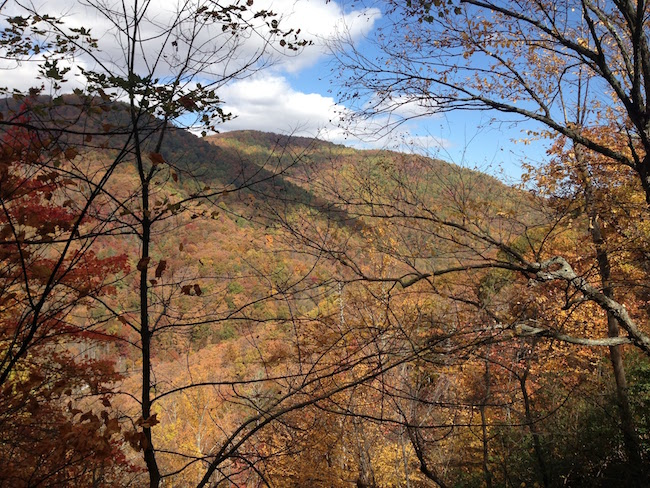
\includegraphics[keepaspectratio]{media/chapter_containers.jpg}}

\begin{quote}
Data needs to be contained within objects so that we can examine,
manipulate, sort, analyze, and communicate about it. In this topic, we
examine some of the more basic
\end{quote}

\section{Lecture Materials}\label{lecture-materials-2}

\begin{quote}
\textbf{Lecture Slides:} Available interactively in the
\href{https://dyerlabteaching.github.io/Data-Containers/slides.html\#/title-slide}{online
version}
\end{quote}

\begin{figure}[H]

{\centering \pandocbounded{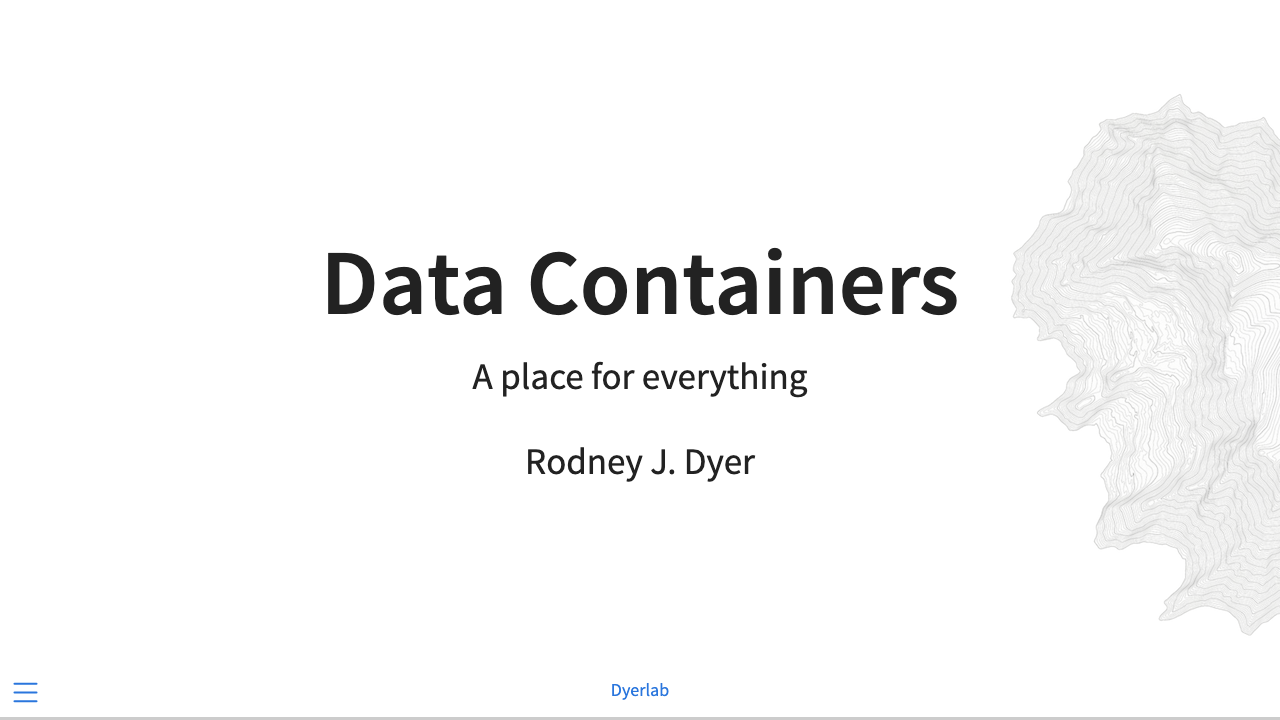
\includegraphics[keepaspectratio]{media/slides_containers.png}}

}

\caption{Lecture Slides}

\end{figure}%

\section{Vectors}\label{vectors}

Vectors are the most basic data container in \texttt{R}. They
\emph{must} contain data of the exact same type and are constructed
using the \texttt{combine()} function, which is abbreviated as
\texttt{c()} because good programmers are lazy programmers. \footnote{The
  more lines of code that you write, the more likely there will be
  either a grammatical error (easier to find) or a logical one (harder
  to find).}

Here is an example with some numbers.

\begin{Shaded}
\begin{Highlighting}[]
\NormalTok{x }\OtherTok{\textless{}{-}} \FunctionTok{c}\NormalTok{(}\DecValTok{1}\NormalTok{,}\DecValTok{2}\NormalTok{,}\DecValTok{3}\NormalTok{)}
\NormalTok{x}
\end{Highlighting}
\end{Shaded}

\begin{verbatim}
[1] 1 2 3
\end{verbatim}

Vectors can contain any of the base data types.

\begin{Shaded}
\begin{Highlighting}[]
\NormalTok{y }\OtherTok{\textless{}{-}} \FunctionTok{c}\NormalTok{(}\ConstantTok{TRUE}\NormalTok{, }\ConstantTok{TRUE}\NormalTok{, }\ConstantTok{FALSE}\NormalTok{, }\ConstantTok{FALSE}\NormalTok{)}
\NormalTok{y}
\end{Highlighting}
\end{Shaded}

\begin{verbatim}
[1]  TRUE  TRUE FALSE FALSE
\end{verbatim}

\begin{Shaded}
\begin{Highlighting}[]
\NormalTok{z }\OtherTok{\textless{}{-}} \FunctionTok{c}\NormalTok{(}\StringTok{"Bob"}\NormalTok{,}\StringTok{"Alice"}\NormalTok{,}\StringTok{"Thomas"}\NormalTok{)}
\NormalTok{z}
\end{Highlighting}
\end{Shaded}

\begin{verbatim}
[1] "Bob"    "Alice"  "Thomas"
\end{verbatim}

Each vector has an inherent length representing the number of elements
it contains.

\begin{Shaded}
\begin{Highlighting}[]
\FunctionTok{length}\NormalTok{(x)}
\end{Highlighting}
\end{Shaded}

\begin{verbatim}
[1] 3
\end{verbatim}

\subsection{Introspection}\label{introspection-1}

When asked, a vector reports the class of itself as the type of data
contained within it.

\begin{Shaded}
\begin{Highlighting}[]
\FunctionTok{class}\NormalTok{(x)}
\end{Highlighting}
\end{Shaded}

\begin{verbatim}
[1] "numeric"
\end{verbatim}

\begin{Shaded}
\begin{Highlighting}[]
\FunctionTok{class}\NormalTok{(y)}
\end{Highlighting}
\end{Shaded}

\begin{verbatim}
[1] "logical"
\end{verbatim}

\begin{Shaded}
\begin{Highlighting}[]
\FunctionTok{class}\NormalTok{(z)}
\end{Highlighting}
\end{Shaded}

\begin{verbatim}
[1] "character"
\end{verbatim}

however, a \texttt{vector} is also a data type. As such, it has the
\texttt{is.vector()} function. So this \texttt{x} can be both a vector
and a numeric.

\begin{Shaded}
\begin{Highlighting}[]
\FunctionTok{is.vector}\NormalTok{( x ) }\SpecialCharTok{\&\&} \FunctionTok{is.numeric}\NormalTok{( x )}
\end{Highlighting}
\end{Shaded}

\begin{verbatim}
[1] TRUE
\end{verbatim}

\subsection{Sequences}\label{sequences}

There are a lot of times when we require a sequnce of values and it
would get a bit tedious to type them all out manually. \texttt{R} has
several options for creating vectors that are comprised of a sequence of
values.

The easiest type is the colon operator, that will generate a seqeunce of
numerical values from the number on the left to the number on the right

\begin{Shaded}
\begin{Highlighting}[]
\DecValTok{1}\SpecialCharTok{:}\DecValTok{10} \OtherTok{{-}\textgreater{}}\NormalTok{ y}
\NormalTok{y}
\end{Highlighting}
\end{Shaded}

\begin{verbatim}
 [1]  1  2  3  4  5  6  7  8  9 10
\end{verbatim}

It also works in the other direction (descending).

\begin{Shaded}
\begin{Highlighting}[]
\DecValTok{10}\SpecialCharTok{:}\DecValTok{1}
\end{Highlighting}
\end{Shaded}

\begin{verbatim}
 [1] 10  9  8  7  6  5  4  3  2  1
\end{verbatim}

However, it is only available to make a sequences where the increment
from one value to the next is \texttt{1}.

\begin{Shaded}
\begin{Highlighting}[]
\FloatTok{3.2}\SpecialCharTok{:}\FloatTok{5.7}
\end{Highlighting}
\end{Shaded}

\begin{verbatim}
[1] 3.2 4.2 5.2
\end{verbatim}

For more fine-grained control, we can use the function \texttt{seq()} to
iterate across a range of values and specify either the step size (here
from 1-10 by 3's)

\begin{Shaded}
\begin{Highlighting}[]
\FunctionTok{seq}\NormalTok{(}\DecValTok{1}\NormalTok{,}\DecValTok{10}\NormalTok{,}\AttributeTok{by=}\DecValTok{3}\NormalTok{)}
\end{Highlighting}
\end{Shaded}

\begin{verbatim}
[1]  1  4  7 10
\end{verbatim}

OR the length of the response and it will figure out the step size to
give you the right number of elements.

\begin{Shaded}
\begin{Highlighting}[]
\FunctionTok{seq}\NormalTok{( }\DecValTok{119}\NormalTok{, }\DecValTok{121}\NormalTok{, }\AttributeTok{length.out =} \DecValTok{6}\NormalTok{)}
\end{Highlighting}
\end{Shaded}

\begin{verbatim}
[1] 119.0 119.4 119.8 120.2 120.6 121.0
\end{verbatim}

\subsection{Indexing \& Access}\label{indexing-access}

To access and change values within a vector, we used square brackets and
the number of the entry of interest. It should be noted that in
\texttt{R}, the first element of a vector is \# 1.

So, to get to the third element of the \texttt{x} vector, we would:

\begin{Shaded}
\begin{Highlighting}[]
\NormalTok{x[}\DecValTok{3}\NormalTok{]}
\end{Highlighting}
\end{Shaded}

\begin{verbatim}
[1] 3
\end{verbatim}

If you ask for values in the vector off the end (e.g., the index is
beyond the length of the vector) it will return missing data.

\begin{Shaded}
\begin{Highlighting}[]
\NormalTok{x[}\DecValTok{5}\NormalTok{]}
\end{Highlighting}
\end{Shaded}

\begin{verbatim}
[1] NA
\end{verbatim}

In addition to getting the values from a vector, assignment of
individual values proceeds similarily.

\begin{Shaded}
\begin{Highlighting}[]
\NormalTok{x[}\DecValTok{2}\NormalTok{] }\OtherTok{\textless{}{-}} \DecValTok{42}
\NormalTok{x}
\end{Highlighting}
\end{Shaded}

\begin{verbatim}
[1]  1 42  3
\end{verbatim}

If you assign a value to a vector that is way off the end, it will fill
in the intermediate values wtih \texttt{NA} for you.

\begin{Shaded}
\begin{Highlighting}[]
\NormalTok{x[}\DecValTok{7}\NormalTok{] }\OtherTok{\textless{}{-}} \DecValTok{43}
\NormalTok{x}
\end{Highlighting}
\end{Shaded}

\begin{verbatim}
[1]  1 42  3 NA NA NA 43
\end{verbatim}

\subsection{Vector Operations}\label{vector-operations}

Just like individual values for each data type, vectors of these data
types can also be operated using the same operators. Consider the two
vectors \texttt{x} (a sequence) and \texttt{y} (a random selection from
a Poisson distribution), both with 5 elements.

\begin{Shaded}
\begin{Highlighting}[]
\NormalTok{x }\OtherTok{\textless{}{-}} \DecValTok{1}\SpecialCharTok{:}\DecValTok{5}
\NormalTok{y }\OtherTok{\textless{}{-}} \FunctionTok{rpois}\NormalTok{(}\DecValTok{5}\NormalTok{,}\DecValTok{2}\NormalTok{)}
\NormalTok{x}
\end{Highlighting}
\end{Shaded}

\begin{verbatim}
[1] 1 2 3 4 5
\end{verbatim}

\begin{Shaded}
\begin{Highlighting}[]
\NormalTok{y}
\end{Highlighting}
\end{Shaded}

\begin{verbatim}
[1] 3 2 1 2 2
\end{verbatim}

Mathematics operations are done element-wise. Here is an example using
addition.

\begin{Shaded}
\begin{Highlighting}[]
\NormalTok{x }\SpecialCharTok{+}\NormalTok{ y }
\end{Highlighting}
\end{Shaded}

\begin{verbatim}
[1] 4 4 4 6 7
\end{verbatim}

as well as exponents.

\begin{Shaded}
\begin{Highlighting}[]
\NormalTok{x}\SpecialCharTok{\^{}}\NormalTok{y}
\end{Highlighting}
\end{Shaded}

\begin{verbatim}
[1]  1  4  3 16 25
\end{verbatim}

If the lengths of the vectors are not the same \texttt{R} will implement
a \emph{recycling rule} where the shorter of the vectors is repeated
until you fill up the size of the longer vector. Here is an example with
the 5-element \texttt{x} and the a new 10-element \texttt{z}. Notice how
the values in x are repeated in the addition operaiton.

\begin{Shaded}
\begin{Highlighting}[]
\NormalTok{z }\OtherTok{\textless{}{-}} \DecValTok{1}\SpecialCharTok{:}\DecValTok{10}
\NormalTok{x }\SpecialCharTok{+}\NormalTok{ z}
\end{Highlighting}
\end{Shaded}

\begin{verbatim}
 [1]  2  4  6  8 10  7  9 11 13 15
\end{verbatim}

If the two vectors are not multiples of each other in length, it will
still recycle the shorter one but will also give you a warning that the
two vectors are not conformant (just a FYI).

\begin{Shaded}
\begin{Highlighting}[]
\NormalTok{x }\SpecialCharTok{+} \DecValTok{1}\SpecialCharTok{:}\DecValTok{8}
\end{Highlighting}
\end{Shaded}

\begin{verbatim}
Warning in x + 1:8: longer object length is not a multiple of shorter object
length
\end{verbatim}

\begin{verbatim}
[1]  2  4  6  8 10  7  9 11
\end{verbatim}

The operations used are dependent upon the base data type. For example,
the following \texttt{character} values can be passed along to the
\texttt{paste()} function to put each of the elements in the first
vectoer with the corresponding values in the second vector (and
specifying the separator).

\begin{Shaded}
\begin{Highlighting}[]
\NormalTok{a }\OtherTok{\textless{}{-}} \FunctionTok{c}\NormalTok{(}\StringTok{"Bob"}\NormalTok{,}\StringTok{"Alice"}\NormalTok{,}\StringTok{"Thomas"}\NormalTok{)}
\NormalTok{b }\OtherTok{\textless{}{-}} \FunctionTok{c}\NormalTok{(}\StringTok{"Biologist"}\NormalTok{,}\StringTok{"Chemist"}\NormalTok{,}\StringTok{"Mathematician"}\NormalTok{)}
\FunctionTok{paste}\NormalTok{( a, b, }\AttributeTok{sep=}\StringTok{" is a "}\NormalTok{)}
\end{Highlighting}
\end{Shaded}

\begin{verbatim}
[1] "Bob is a Biologist"        "Alice is a Chemist"       
[3] "Thomas is a Mathematician"
\end{verbatim}

So, in addition to being able to work on individual values, \emph{all
functions are also vector functions}.

\section{Matrices}\label{matrices}

A \texttt{matrix} is a 2-dimensional container for the same kind of data
as well. The two dimensions are represented as \emph{rows} and
\emph{columns} in a rectangular configuration. Here I will make a 3x3
vector consisting of a sequence of numbers from 1 to 9.

\begin{Shaded}
\begin{Highlighting}[]
\NormalTok{X }\OtherTok{\textless{}{-}} \FunctionTok{matrix}\NormalTok{( }\DecValTok{1}\SpecialCharTok{:}\DecValTok{9}\NormalTok{, }\AttributeTok{nrow=}\DecValTok{3}\NormalTok{, }\AttributeTok{ncol=}\DecValTok{3}\NormalTok{ )}
\NormalTok{X}
\end{Highlighting}
\end{Shaded}

\begin{verbatim}
     [,1] [,2] [,3]
[1,]    1    4    7
[2,]    2    5    8
[3,]    3    6    9
\end{verbatim}

It is a bit redundant to have both \texttt{nrow} and \texttt{ncol} with
\texttt{nrow\ *\ ncol\ =\ length(sequence)}, you can just specify one of
them and it will work out the other dimension.

\subsection{Indexing}\label{indexing}

Just like a vector, matrices use square brackets and the row \& column
number (in that order) to access indiviudal elements. Also, just like
vectors, both rows and columns start at 1 (not zero). So to replace the
value in the second row and second column with the number \texttt{42},
we do this.

\begin{Shaded}
\begin{Highlighting}[]
\NormalTok{X[}\DecValTok{2}\NormalTok{,}\DecValTok{2}\NormalTok{] }\OtherTok{\textless{}{-}} \DecValTok{42}
\NormalTok{X}
\end{Highlighting}
\end{Shaded}

\begin{verbatim}
     [,1] [,2] [,3]
[1,]    1    4    7
[2,]    2   42    8
[3,]    3    6    9
\end{verbatim}

Matrices are actually structures fundamental to things like linear
algebra. As such, there are many operations that can be applied to
matrices, both unary and binary.

A \emph{transpose} is a translation of a matrix that switches the rows
and columns. In \texttt{R} it is done by the function \texttt{t()}. Here
I use this to define another matrix.

\begin{Shaded}
\begin{Highlighting}[]
\NormalTok{Y }\OtherTok{\textless{}{-}} \FunctionTok{t}\NormalTok{(X)}
\NormalTok{Y}
\end{Highlighting}
\end{Shaded}

\begin{verbatim}
     [,1] [,2] [,3]
[1,]    1    2    3
[2,]    4   42    6
[3,]    7    8    9
\end{verbatim}

Binary operators using the normal operators in the top row of your
keyboard are generally element-wise operations. Here the addition of
these two matrices require:\\
1. Both matrices have the same number of rows.\\
2. Both matrices have the same number of columns.\\
3. Both matrices have the same internal data types.

Here is an example of addition (notic how the resulting {[}1,1{]} object
is equal to X{[}1,1{]} + Y{[}1,1{]})

\begin{Shaded}
\begin{Highlighting}[]
\NormalTok{X }\SpecialCharTok{+}\NormalTok{ Y}
\end{Highlighting}
\end{Shaded}

\begin{verbatim}
     [,1] [,2] [,3]
[1,]    2    6   10
[2,]    6   84   14
[3,]   10   14   18
\end{verbatim}

The same for element-wise multiplication.

\begin{Shaded}
\begin{Highlighting}[]
\NormalTok{X }\SpecialCharTok{*}\NormalTok{ Y}
\end{Highlighting}
\end{Shaded}

\begin{verbatim}
     [,1] [,2] [,3]
[1,]    1    8   21
[2,]    8 1764   48
[3,]   21   48   81
\end{verbatim}

However, there is another kind of matrix mutliplication that sums the
product or rows and columns. Since this is also a variety of
multiplication but is carried out differently, we need to use a
different operator. Here the matrix mutliplication operator is denoted
as the combination of characters \texttt{\%*\%}.

\begin{Shaded}
\begin{Highlighting}[]
\NormalTok{X }\SpecialCharTok{\%*\%}\NormalTok{ Y}
\end{Highlighting}
\end{Shaded}

\begin{verbatim}
     [,1] [,2] [,3]
[1,]   66  226   90
[2,]  226 1832  330
[3,]   90  330  126
\end{verbatim}

This operation has a few different constraints:

\begin{enumerate}
\def\labelenumi{\arabic{enumi}.}
\tightlist
\item
  The number of columns in the left matrix must equal the number of rows
  in the right one.
\item
  The resulting matrix will have the number of rows equal to that of the
  right matrix.
\item
  The resulting matrix will have the number of columns equal to that of
  the left matrix.
\item
  The resulting element at the \(i\) \(j\) position is the sum of the
  multipliation of the elements in the \(i^{th}\) row of the left matrix
  and the \(j^{th}\) column of the right one.
\end{enumerate}

So the resulting element in \texttt{{[}1,3{]}} position is found by
\(1*3 + 4*6 + 7*9 = 90\).

\section{Lists}\label{lists}

Lists are a more flexible container type. Here, lists can contain
different types of data in a single list. Here is an example of a list
made with a few \texttt{character} vluaes, a \texttt{numeric}, a
\texttt{constant}, and a \texttt{logical} value.

\begin{Shaded}
\begin{Highlighting}[]
\NormalTok{lst }\OtherTok{\textless{}{-}} \FunctionTok{list}\NormalTok{(}\StringTok{"A"}\NormalTok{,}\StringTok{"B"}\NormalTok{,}\FloatTok{323423.3}\NormalTok{, pi, }\ConstantTok{TRUE}\NormalTok{)}
\end{Highlighting}
\end{Shaded}

When you print out a list made like this, it will indicate each element
as a numeric value in \textbf{double square brackets}.

\begin{Shaded}
\begin{Highlighting}[]
\NormalTok{lst}
\end{Highlighting}
\end{Shaded}

\begin{verbatim}
[[1]]
[1] "A"

[[2]]
[1] "B"

[[3]]
[1] 323423.3

[[4]]
[1] 3.141593

[[5]]
[1] TRUE
\end{verbatim}

\subsection{Indexing}\label{indexing-1}

Indexing values in a list can be done using these numbers. To get and
reset the values in the second element of the list, one would:

\begin{Shaded}
\begin{Highlighting}[]
\NormalTok{lst[[}\DecValTok{2}\NormalTok{]] }\OtherTok{\textless{}{-}} \StringTok{"C"}
\NormalTok{lst}
\end{Highlighting}
\end{Shaded}

\begin{verbatim}
[[1]]
[1] "A"

[[2]]
[1] "C"

[[3]]
[1] 323423.3

[[4]]
[1] 3.141593

[[5]]
[1] TRUE
\end{verbatim}

\subsection{Named Lists}\label{named-lists}

Lists can be more valuable if we use names for the \emph{keys} instead
of just numbers. Here, I make an empty list and then assign values to it
using names (as character values) in square brakets.

\begin{Shaded}
\begin{Highlighting}[]
\NormalTok{myInfo }\OtherTok{\textless{}{-}} \FunctionTok{list}\NormalTok{()}
\NormalTok{myInfo[}\StringTok{"First Name"}\NormalTok{] }\OtherTok{\textless{}{-}} \StringTok{"Rodney"}
\NormalTok{myInfo[}\StringTok{"Second Name"}\NormalTok{] }\OtherTok{\textless{}{-}} \StringTok{"Dyer"}
\NormalTok{myInfo[}\StringTok{"Favorite Number"}\NormalTok{] }\OtherTok{\textless{}{-}} \DecValTok{42}
\end{Highlighting}
\end{Shaded}

When showing named lists, it prints included items as:

\begin{Shaded}
\begin{Highlighting}[]
\NormalTok{myInfo}
\end{Highlighting}
\end{Shaded}

\begin{verbatim}
$`First Name`
[1] "Rodney"

$`Second Name`
[1] "Dyer"

$`Favorite Number`
[1] 42
\end{verbatim}

In addition to the square bracket approach, we can also use as \$
notation to add elements to the list (like shown above).

\begin{Shaded}
\begin{Highlighting}[]
\NormalTok{myInfo}\SpecialCharTok{$}\NormalTok{Vegitarian }\OtherTok{\textless{}{-}} \ConstantTok{FALSE}
\end{Highlighting}
\end{Shaded}

Both are equivallent.

\begin{Shaded}
\begin{Highlighting}[]
\NormalTok{myInfo}
\end{Highlighting}
\end{Shaded}

\begin{verbatim}
$`First Name`
[1] "Rodney"

$`Second Name`
[1] "Dyer"

$`Favorite Number`
[1] 42

$Vegitarian
[1] FALSE
\end{verbatim}

In addition to having different data types, you can also have different
sized data types inside a list. Here I add a vector (a valid data type
as shown above) to the list.

\begin{Shaded}
\begin{Highlighting}[]
\NormalTok{myInfo}\SpecialCharTok{$}\NormalTok{Homes }\OtherTok{\textless{}{-}} \FunctionTok{c}\NormalTok{(}\StringTok{"RVA"}\NormalTok{,}\StringTok{"Oly"}\NormalTok{,}\StringTok{"SEA"}\NormalTok{)}
\NormalTok{myInfo}
\end{Highlighting}
\end{Shaded}

\begin{verbatim}
$`First Name`
[1] "Rodney"

$`Second Name`
[1] "Dyer"

$`Favorite Number`
[1] 42

$Vegitarian
[1] FALSE

$Homes
[1] "RVA" "Oly" "SEA"
\end{verbatim}

To access these values, we can use a combination of \$ notation and
\texttt{{[}{]}} on the resulting vector.

\begin{Shaded}
\begin{Highlighting}[]
\NormalTok{myInfo}\SpecialCharTok{$}\NormalTok{Homes[}\DecValTok{2}\NormalTok{]}
\end{Highlighting}
\end{Shaded}

\begin{verbatim}
[1] "Oly"
\end{verbatim}

When elements in a list are defined using named keys, the list itself
can be asked for the keys using \texttt{names()}.

\begin{Shaded}
\begin{Highlighting}[]
\FunctionTok{names}\NormalTok{(myInfo)}
\end{Highlighting}
\end{Shaded}

\begin{verbatim}
[1] "First Name"      "Second Name"     "Favorite Number" "Vegitarian"     
[5] "Homes"          
\end{verbatim}

This can be helpful at times when you did not create the list yourself
and want to see what is inside of them.

\subsection{Spaces in Names}\label{spaces-in-names}

As you see above, this list has \emph{keys} such as ``First Name'' and
``Vegitarian''. The first one has a \emph{space} inside of it whereas
the second one does not. This is a challenge. If we were to try to use
the first key as

\begin{Shaded}
\begin{Highlighting}[]
\NormalTok{myInfo}\SpecialCharTok{$}\NormalTok{First Name}
\end{Highlighting}
\end{Shaded}

Would give you an error (if I ran the chunck but I cannot because it is
an error and won't let me compile this document if I do). For names that
have spaces, we need to enclose them inside back-ticks (as shown in the
output above).

\begin{Shaded}
\begin{Highlighting}[]
\NormalTok{myInfo}\SpecialCharTok{$}\StringTok{\textasciigrave{}}\AttributeTok{First Name}\StringTok{\textasciigrave{}}
\end{Highlighting}
\end{Shaded}

\begin{verbatim}
[1] "Rodney"
\end{verbatim}

So feel free to use names that make sense, but if you do, you'll need to
treat them a bit specially using the backticks.

\subsection{Analysis Output}\label{analysis-output}

By far, the most common location for lists is when you do some kind of
analysis. Almost all analyses return the restuls as a special kind of
list.

Here is an example looking at some data from three species of Iris on
the lengths and width of sepal and petals. The data look like:

\begin{figure}[H]

\centering{

\pandocbounded{
\includegraphics[keepaspectratio]{narrative_containers_files/figure-pdf/fig-iris-1.pdf}}

}

\caption{\label{fig-iris}The distribution of sepal and petal lengths
from three species of Iris.}

\end{figure}%

We can look at the correlation between two variable using the built-in
\texttt{cor.test()} function.

\begin{Shaded}
\begin{Highlighting}[]
\NormalTok{iris.test }\OtherTok{\textless{}{-}} \FunctionTok{cor.test}\NormalTok{( iris}\SpecialCharTok{$}\NormalTok{Sepal.Length, iris}\SpecialCharTok{$}\NormalTok{Petal.Length )}
\end{Highlighting}
\end{Shaded}

We can print the output and it will format the results in a proper way.

\begin{Shaded}
\begin{Highlighting}[]
\NormalTok{iris.test}
\end{Highlighting}
\end{Shaded}

\begin{verbatim}

    Pearson's product-moment correlation

data:  iris$Sepal.Length and iris$Petal.Length
t = 21.646, df = 148, p-value < 2.2e-16
alternative hypothesis: true correlation is not equal to 0
95 percent confidence interval:
 0.8270363 0.9055080
sample estimates:
      cor 
0.8717538 
\end{verbatim}

However, the elements in the \texttt{iris.test} are simply a list.

\begin{Shaded}
\begin{Highlighting}[]
\FunctionTok{names}\NormalTok{(iris.test)}
\end{Highlighting}
\end{Shaded}

\begin{verbatim}
[1] "statistic"   "parameter"   "p.value"     "estimate"    "null.value" 
[6] "alternative" "method"      "data.name"   "conf.int"   
\end{verbatim}

If fact, the contents of the output are just keys and values, even
though when we printed it all out, it was formatted as a much more
informative output.

{\def\LTcaptype{none} % do not increment counter
\begin{longtable}[]{@{}ll@{}}
\toprule\noalign{}
& Values \\
\midrule\noalign{}
\endhead
\bottomrule\noalign{}
\endlastfoot
statistic.t & 21.6460193457598 \\
parameter.df & 148 \\
p.value & 1.03866741944975e-47 \\
estimate.cor & 0.871753775886583 \\
null.value.correlation & 0 \\
alternative & two.sided \\
method & Pearson's product-moment correlation \\
data.name & iris\(Sepal.Length and iris\)Petal.Length \\
conf.int1 & 0.827036329664362 \\
conf.int2 & 0.905508048821454 \\
\end{longtable}
}

We will come back to this special kind of printing later when discussing
functions but for now, lets just consider how cool this is because we
can access the raw values of the analysis directly. We an also easily
incorporate the findings of analyses, such as this simple correlation
test, and insert the content into the text. All you have to do is
address the components of the analysis as in-text r citation. Here is an
example where I include the values of:

\begin{Shaded}
\begin{Highlighting}[]
\NormalTok{iris.test}\SpecialCharTok{$}\NormalTok{estimate}
\end{Highlighting}
\end{Shaded}

\begin{verbatim}
      cor 
0.8717538 
\end{verbatim}

\begin{Shaded}
\begin{Highlighting}[]
\NormalTok{iris.test}\SpecialCharTok{$}\NormalTok{statistic}
\end{Highlighting}
\end{Shaded}

\begin{verbatim}
       t 
21.64602 
\end{verbatim}

\begin{Shaded}
\begin{Highlighting}[]
\NormalTok{iris.test}\SpecialCharTok{$}\NormalTok{p.value}
\end{Highlighting}
\end{Shaded}

\begin{verbatim}
[1] 1.038667e-47
\end{verbatim}

Here is an example paragraph (see the raw quarto document to see the
formatting).

\begin{quote}
There was a significant relationship between sepal and petal length
(Pearson Correlation, \(\rho =\) 0.872, \(t =\) 21.6, P = 1.04e-47).
\end{quote}

\section{Data Frames}\label{data-frames}

The \texttt{data.frame} is the most common container for all the data
you'll be working with in \texttt{R}. It is \emph{kind of} like a
spreadsheet in that each column of data is the same kind of data
measured on all objects (e.g., weight, survival, population, etc.) and
each row represents one observation that has a bunch of different kinds
of measurements associated with it.

Here is an example with three different data types (the z is a random
sample of TRUE/FALSE equal in length to the other elements).

\begin{Shaded}
\begin{Highlighting}[]
\NormalTok{x }\OtherTok{\textless{}{-}} \DecValTok{1}\SpecialCharTok{:}\DecValTok{10}
\NormalTok{y }\OtherTok{\textless{}{-}}\NormalTok{ LETTERS[}\DecValTok{11}\SpecialCharTok{:}\DecValTok{20}\NormalTok{]}
\NormalTok{z }\OtherTok{\textless{}{-}} \FunctionTok{sample}\NormalTok{( }\FunctionTok{c}\NormalTok{(}\ConstantTok{TRUE}\NormalTok{,}\ConstantTok{FALSE}\NormalTok{), }\AttributeTok{size=}\DecValTok{10}\NormalTok{, }\AttributeTok{replace=}\ConstantTok{TRUE}\NormalTok{ )}
\end{Highlighting}
\end{Shaded}

I can put them into a \texttt{data.frame} object as:

\begin{Shaded}
\begin{Highlighting}[]
\NormalTok{df }\OtherTok{\textless{}{-}} \FunctionTok{data.frame}\NormalTok{( }\AttributeTok{TheNums =}\NormalTok{ x,}
                  \AttributeTok{TheLetters =}\NormalTok{ y,}
                  \AttributeTok{TF =}\NormalTok{ z}
\NormalTok{                  )}
\NormalTok{df}
\end{Highlighting}
\end{Shaded}

\begin{verbatim}
   TheNums TheLetters    TF
1        1          K FALSE
2        2          L  TRUE
3        3          M  TRUE
4        4          N  TRUE
5        5          O FALSE
6        6          P  TRUE
7        7          Q FALSE
8        8          R FALSE
9        9          S  TRUE
10      10          T  TRUE
\end{verbatim}

Since each column is its own `type' we can easily get a summary of the
elements within it using \texttt{summary()}.

\begin{Shaded}
\begin{Highlighting}[]
\FunctionTok{summary}\NormalTok{( df )}
\end{Highlighting}
\end{Shaded}

\begin{verbatim}
    TheNums       TheLetters            TF         
 Min.   : 1.00   Length:10          Mode :logical  
 1st Qu.: 3.25   Class :character   FALSE:4        
 Median : 5.50   Mode  :character   TRUE :6        
 Mean   : 5.50                                     
 3rd Qu.: 7.75                                     
 Max.   :10.00                                     
\end{verbatim}

And depending upon the data type, the output may give numerical, counts,
or just description of the contents.

\subsection{Indexing}\label{indexing-2}

Just like a list, a \texttt{data.frame} can be defined as having named
columns. The distinction here is that each column should have the same
number of elements in it, whereas a list may have differnet lengths to
the elements.

\begin{Shaded}
\begin{Highlighting}[]
\FunctionTok{names}\NormalTok{( df )}
\end{Highlighting}
\end{Shaded}

\begin{verbatim}
[1] "TheNums"    "TheLetters" "TF"        
\end{verbatim}

And like the list, we can easily use the \$ operator to access the
vectors components.

\begin{Shaded}
\begin{Highlighting}[]
\NormalTok{df}\SpecialCharTok{$}\NormalTok{TheLetters}
\end{Highlighting}
\end{Shaded}

\begin{verbatim}
 [1] "K" "L" "M" "N" "O" "P" "Q" "R" "S" "T"
\end{verbatim}

\begin{Shaded}
\begin{Highlighting}[]
\FunctionTok{class}\NormalTok{( df}\SpecialCharTok{$}\NormalTok{TheLetters )}
\end{Highlighting}
\end{Shaded}

\begin{verbatim}
[1] "character"
\end{verbatim}

Indexing and grabbing elements can be done by either the column name
(with \$) and a square bracket OR by the \texttt{{[}row,col{]}} indexing
like the matrix above.

\begin{Shaded}
\begin{Highlighting}[]
\NormalTok{df}\SpecialCharTok{$}\NormalTok{TheLetters[}\DecValTok{3}\NormalTok{]}
\end{Highlighting}
\end{Shaded}

\begin{verbatim}
[1] "M"
\end{verbatim}

\begin{Shaded}
\begin{Highlighting}[]
\NormalTok{df[}\DecValTok{3}\NormalTok{,}\DecValTok{2}\NormalTok{]}
\end{Highlighting}
\end{Shaded}

\begin{verbatim}
[1] "M"
\end{verbatim}

Just like a matrix, the dimensions of the \texttt{data.frame} is defined
by the number of rows and columns.

\begin{Shaded}
\begin{Highlighting}[]
\FunctionTok{dim}\NormalTok{( df )}
\end{Highlighting}
\end{Shaded}

\begin{verbatim}
[1] 10  3
\end{verbatim}

\begin{Shaded}
\begin{Highlighting}[]
\FunctionTok{nrow}\NormalTok{( df )}
\end{Highlighting}
\end{Shaded}

\begin{verbatim}
[1] 10
\end{verbatim}

\begin{Shaded}
\begin{Highlighting}[]
\FunctionTok{ncol}\NormalTok{( df )}
\end{Highlighting}
\end{Shaded}

\begin{verbatim}
[1] 3
\end{verbatim}

\subsection{Loading Data}\label{loading-data}

By far, you will most often NOT be making data by hand but instead will
be loading it from external locations. here is an example of how we can
load in a CSV file that is located in the GitHub repository for this
topic. As this is a public repository, we can get a direct URL to the
file. For simplicity, I'll load in tidyverse and use some helper
functions contained therein.

\begin{Shaded}
\begin{Highlighting}[]
\FunctionTok{library}\NormalTok{( tidyverse )}
\end{Highlighting}
\end{Shaded}

\begin{verbatim}
-- Attaching core tidyverse packages ------------------------ tidyverse 2.0.0 --
v dplyr     1.2.1     v readr     2.2.0
v forcats   1.0.1     v stringr   1.6.0
v lubridate 1.9.5     v tibble    3.3.1
v purrr     1.2.1     v tidyr     1.3.2
-- Conflicts ------------------------------------------ tidyverse_conflicts() --
x dplyr::filter() masks stats::filter()
x dplyr::lag()    masks stats::lag()
i Use the conflicted package (<http://conflicted.r-lib.org/>) to force all conflicts to become errors
\end{verbatim}

The URL for this repository is

\begin{Shaded}
\begin{Highlighting}[]
\NormalTok{url }\OtherTok{\textless{}{-}} \StringTok{"https://raw.githubusercontent.com/DyerlabTeaching/Data{-}Containers/main/data/arapat.csv"}
\end{Highlighting}
\end{Shaded}

And we can read it in directly (as long as we have an internet
connection) as:

\begin{Shaded}
\begin{Highlighting}[]
\NormalTok{beetles }\OtherTok{\textless{}{-}} \FunctionTok{read\_csv}\NormalTok{( url )}
\end{Highlighting}
\end{Shaded}

\begin{verbatim}
Rows: 39 Columns: 3
-- Column specification --------------------------------------------------------
Delimiter: ","
chr (1): Stratum
dbl (2): Longitude, Latitude

i Use `spec()` to retrieve the full column specification for this data.
i Specify the column types or set `show_col_types = FALSE` to quiet this message.
\end{verbatim}

Notice how the funtion tells us a few things about the data.

The data itself consists of:

\begin{Shaded}
\begin{Highlighting}[]
\FunctionTok{summary}\NormalTok{( beetles )}
\end{Highlighting}
\end{Shaded}

\begin{verbatim}
   Stratum            Longitude         Latitude    
 Length:39          Min.   :-114.3   Min.   :23.08  
 Class :character   1st Qu.:-112.9   1st Qu.:24.52  
 Mode  :character   Median :-111.5   Median :26.21  
                    Mean   :-111.7   Mean   :26.14  
                    3rd Qu.:-110.4   3rd Qu.:27.47  
                    Max.   :-109.1   Max.   :29.33  
\end{verbatim}

which looks like:

\begin{Shaded}
\begin{Highlighting}[]
\NormalTok{beetles}
\end{Highlighting}
\end{Shaded}

\begin{verbatim}
# A tibble: 39 x 3
   Stratum Longitude Latitude
   <chr>       <dbl>    <dbl>
 1 88          -114.     29.3
 2 9           -114.     29.0
 3 84          -114.     29.0
 4 175         -113.     28.7
 5 177         -114.     28.7
 6 173         -113.     28.4
 7 171         -113.     28.2
 8 89          -113.     28.0
 9 159         -113.     27.5
10 SFr         -113.     27.4
# i 29 more rows
\end{verbatim}

We can quickly use these data and make an interactive labeled map of it
in a few lines of code (click on a marker).

\begin{figure}[H]

{\centering \pandocbounded{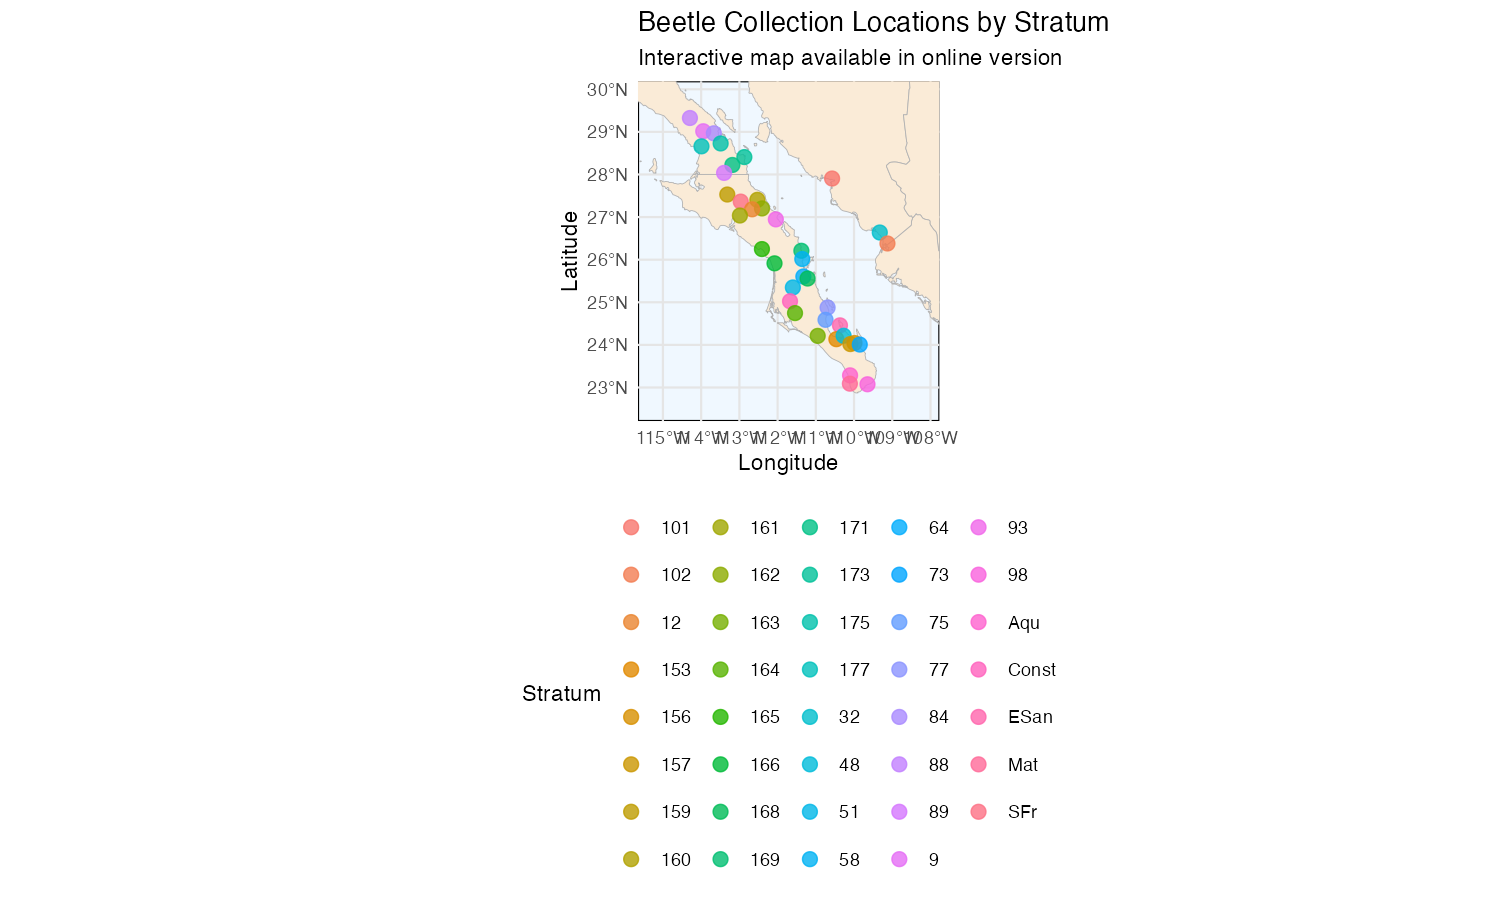
\includegraphics[keepaspectratio]{media/map_containers_leaflet.png}}

}

\caption{Beetle Collection Locations by Stratum - Interactive map
available in online version}

\end{figure}%

\chapter{Tidyverse}\label{tidyverse}

\pandocbounded{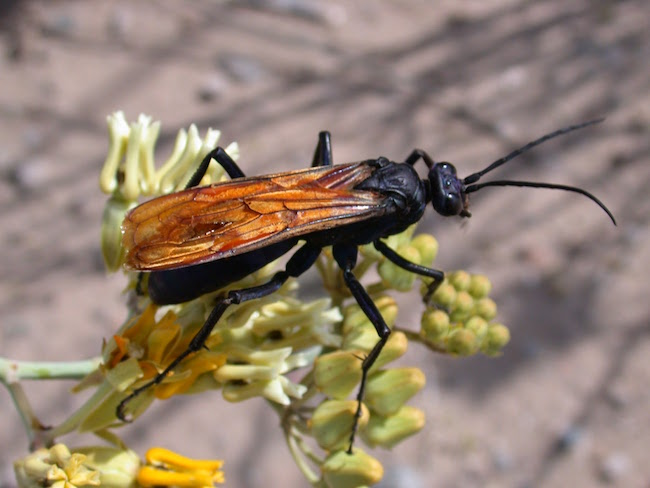
\includegraphics[keepaspectratio]{media/chapter_tidyverse.jpg}}

\begin{quote}
The ability to quickly and easily manipulate and rework data is the base
foundation for all the work you will be doing in \texttt{R}. There is no
more fundamental (and important) skill required than being able to
quickly and easily take raw data and reconfigure it properly for
inclusion into an analysis, summary, graphic, or table. Using features
of the \texttt{tidyverse} library are key.
\end{quote}

\section{Lecture Materials}\label{lecture-materials-3}

\begin{quote}
\textbf{Lecture Slides:} Available interactively in the
\href{https://dyerlabteaching.github.io/Tidyverse/slides.html\#/title-slide}{online
version}
\end{quote}

\begin{figure}[H]

{\centering \pandocbounded{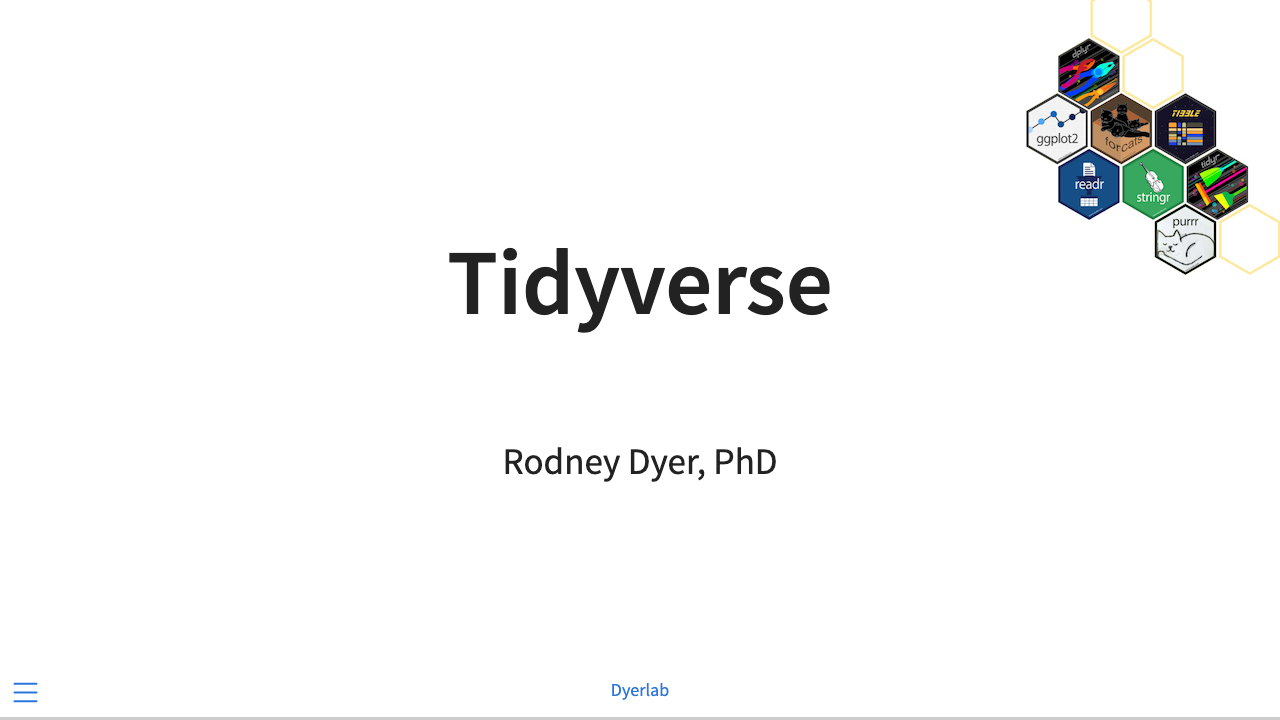
\includegraphics[keepaspectratio]{media/slides_tidyverse.png}}

}

\caption{Lecture Slides}

\end{figure}%

\section{The Tidyverse Approach}\label{the-tidyverse-approach}

This is the first introduction to tidyverse and is the key skill
necessary to become proficient at data analysis.

\begin{Shaded}
\begin{Highlighting}[]
\FunctionTok{library}\NormalTok{( tidyverse )}
\end{Highlighting}
\end{Shaded}

\begin{verbatim}
-- Attaching core tidyverse packages ------------------------ tidyverse 2.0.0 --
v dplyr     1.2.1     v readr     2.2.0
v forcats   1.0.1     v stringr   1.6.0
v ggplot2   4.0.2     v tibble    3.3.1
v lubridate 1.9.5     v tidyr     1.3.2
v purrr     1.2.1     
-- Conflicts ------------------------------------------ tidyverse_conflicts() --
x dplyr::filter() masks stats::filter()
x dplyr::lag()    masks stats::lag()
i Use the conflicted package (<http://conflicted.r-lib.org/>) to force all conflicts to become errors
\end{verbatim}

\begin{Shaded}
\begin{Highlighting}[]
\FunctionTok{library}\NormalTok{( lubridate )}
\end{Highlighting}
\end{Shaded}

\subsection{The Data}\label{the-data}

For this topic we will use some example data from the
\href{https://ricerivers.vcu.edu}{Rice Rivers Center}. These data
represent both atmospheric and water data collected from instrumentation
on-site. I have stored these data in a spreadsheet that is shared on
Google Drive as a CSV file.

You can look at it
\href{https://docs.google.com/spreadsheets/d/1Mk1YGH9LqjF7drJE-td1G_JkdADOU0eMlrP01WFBT8s}{here}.

\subsection{\texorpdfstring{The Data in
\texttt{R}}{The Data in R}}\label{the-data-in-r}

So let's load it into memory and take a look at it.

\begin{Shaded}
\begin{Highlighting}[]
\NormalTok{url }\OtherTok{\textless{}{-}} \StringTok{"https://docs.google.com/spreadsheets/d/1Mk1YGH9LqjF7drJE{-}td1G\_JkdADOU0eMlrP01WFBT8s/pub?gid=0\&single=true\&output=csv"}
\NormalTok{rice }\OtherTok{\textless{}{-}} \FunctionTok{read\_csv}\NormalTok{( url )}
\end{Highlighting}
\end{Shaded}

\begin{verbatim}
Rows: 8199 Columns: 23
-- Column specification --------------------------------------------------------
Delimiter: ","
chr  (1): DateTime
dbl (22): RecordID, PAR, WindSpeed_mph, WindDir, AirTempF, RelHumidity, BP_H...

i Use `spec()` to retrieve the full column specification for this data.
i Specify the column types or set `show_col_types = FALSE` to quiet this message.
\end{verbatim}

\begin{Shaded}
\begin{Highlighting}[]
\FunctionTok{summary}\NormalTok{( rice )}
\end{Highlighting}
\end{Shaded}

\begin{verbatim}
   DateTime            RecordID          PAR           WindSpeed_mph   
 Length:8199        Min.   :43816   Min.   :   0.000   Min.   : 0.000  
 Class :character   1st Qu.:45866   1st Qu.:   0.000   1st Qu.: 2.467  
 Mode  :character   Median :47915   Median :   0.046   Median : 4.090  
                    Mean   :47915   Mean   : 241.984   Mean   : 5.446  
                    3rd Qu.:49964   3rd Qu.: 337.900   3rd Qu.: 7.292  
                    Max.   :52014   Max.   :1957.000   Max.   :30.650  
                                                                       
    WindDir          AirTempF       RelHumidity        BP_HG      
 Min.   :  0.00   Min.   : 3.749   Min.   :15.37   Min.   :29.11  
 1st Qu.: 37.31   1st Qu.:31.545   1st Qu.:42.25   1st Qu.:29.87  
 Median :137.30   Median :37.440   Median :56.40   Median :30.01  
 Mean   :146.20   Mean   :38.795   Mean   :58.37   Mean   :30.02  
 3rd Qu.:249.95   3rd Qu.:46.410   3rd Qu.:76.59   3rd Qu.:30.21  
 Max.   :360.00   Max.   :74.870   Max.   :93.00   Max.   :30.58  
                                                                  
    Rain_in            H2O_TempC       SpCond_mScm      Salinity_ppt   
 Min.   :0.0000000   Min.   :-0.140   Min.   :0.0110   Min.   :0.0000  
 1st Qu.:0.0000000   1st Qu.: 3.930   1st Qu.:0.1430   1st Qu.:0.0700  
 Median :0.0000000   Median : 5.450   Median :0.1650   Median :0.0800  
 Mean   :0.0008412   Mean   : 5.529   Mean   :0.1611   Mean   :0.0759  
 3rd Qu.:0.0000000   3rd Qu.: 7.410   3rd Qu.:0.1760   3rd Qu.:0.0800  
 Max.   :0.3470000   Max.   :13.300   Max.   :0.2110   Max.   :0.1000  
                     NA's   :1        NA's   :1        NA's   :1       
       PH           PH_mv        Turbidity_ntu       Chla_ugl    
 Min.   :6.43   Min.   :-113.8   Min.   :  6.20   Min.   :  1.3  
 1st Qu.:7.50   1st Qu.: -47.8   1st Qu.: 15.50   1st Qu.:  3.7  
 Median :7.58   Median : -43.8   Median : 21.80   Median :  6.7  
 Mean   :7.60   Mean   : -44.5   Mean   : 24.54   Mean   :137.3  
 3rd Qu.:7.69   3rd Qu.: -38.9   3rd Qu.: 30.30   3rd Qu.:302.6  
 Max.   :9.00   Max.   :  28.5   Max.   :187.70   Max.   :330.1  
 NA's   :1      NA's   :1        NA's   :1        NA's   :1      
   BGAPC_CML        BGAPC_rfu         ODO_sat         ODO_mgl     
 Min.   :   188   Min.   :  0.10   Min.   : 87.5   Min.   :10.34  
 1st Qu.:   971   1st Qu.:  0.50   1st Qu.: 99.2   1st Qu.:12.34  
 Median :  1369   Median :  0.70   Median :101.8   Median :12.88  
 Mean   :153571   Mean   : 72.91   Mean   :102.0   Mean   :12.88  
 3rd Qu.:345211   3rd Qu.:163.60   3rd Qu.:104.1   3rd Qu.:13.34  
 Max.   :345471   Max.   :163.70   Max.   :120.8   Max.   :14.99  
 NA's   :1        NA's   :1        NA's   :1       NA's   :1      
    Depth_ft        Depth_m      SurfaceWaterElev_m_levelNad83m
 Min.   :12.15   Min.   :3.705   Min.   :-32.53                
 1st Qu.:14.60   1st Qu.:4.451   1st Qu.:-31.78                
 Median :15.37   Median :4.684   Median :-31.55                
 Mean   :15.34   Mean   :4.677   Mean   :-31.55                
 3rd Qu.:16.12   3rd Qu.:4.913   3rd Qu.:-31.32                
 Max.   :17.89   Max.   :5.454   Max.   :-30.78                
                                                               
\end{verbatim}

These data represent measurements taken every 15 minutes, 24 hours a
day, 7 days a week, 365 days a year. For brevity, this file contains
measurements starting at 1/1/2014 12:00:00 AM and ending at 3/27/2014
9:30:00 AM (only 8199 records here\ldots).

If you look at the summary of the data above, you will see several
things, including:

\begin{itemize}
\tightlist
\item
  Date and time objects are \texttt{character}
\item
  Some measurements are in Standard and some in Imperial with units in
  the same file include both °F and °C, as well as measurements in
  meters, feet, and inches. In fact, there are duplication of data
  columns in different units (guess what kind of correlation they might
  have\ldots)
\end{itemize}

\section{Verbs of Analysis}\label{verbs-of-analysis}

When we perform any type of data manipulation, we use specific verbs.
There is a limited lexicon for us to use, but the key here is how we
perform these actions, and in which order they are deployed for a huge
diversity in outcomes. For now, these basic verbs include:

\begin{itemize}
\tightlist
\item
  \emph{Select:} Used to grab or reorder columns of data.
\item
  \emph{Filter:} Used to grab subsets of records (rows) based upon some
  criteria.
\item
  \emph{Mutate:} Create new columns of data based upon manipulations of
  existing columns.
\item
  \emph{Arrange:} Order the records (rows) based upon some criteria.
\item
  \emph{Group:} Gather records together to perform operations on chunks
  of them similar to \texttt{by()}.
\item
  \emph{Summarize:} Extract summaries of data (or grouped data) based
  upon some defined criteria.
\end{itemize}

In the following examples, we'll be using the rice data above. For each
verb, I'm going to use the pipe operator (\texttt{\%\textgreater{}\%})
to send the data into the example functions and then assign the result
to a dummy \texttt{data.frame} named \texttt{df}. The arguments passed
to each of the verbs are where the magic happens.

\subsection{The Output}\label{the-output}

The key to these activities is that every one of these functions takes a
\texttt{data.frame} as input, does its operations on it, then return a
\texttt{data.frame} object as output. The \texttt{data.frame} is the
core data container for all of these actions.

\subsection{Select Operator}\label{select-operator}

The \texttt{select()} function allows you to choose which columns of
data to work with.

\begin{Shaded}
\begin{Highlighting}[]
\NormalTok{rice }\SpecialCharTok{\%\textgreater{}\%}
  \FunctionTok{select}\NormalTok{( DateTime, AirTempF ) }\OtherTok{{-}\textgreater{}}\NormalTok{ df }
\FunctionTok{head}\NormalTok{(df)}
\end{Highlighting}
\end{Shaded}

\begin{verbatim}
# A tibble: 6 x 2
  DateTime             AirTempF
  <chr>                   <dbl>
1 1/1/2014 12:00:00 AM     31.0
2 1/1/2014 12:15:00 AM     30.7
3 1/1/2014 12:30:00 AM     31.2
4 1/1/2014 12:45:00 AM     30.5
5 1/1/2014 1:00:00 AM      30.9
6 1/1/2014 1:15:00 AM      30.6
\end{verbatim}

Select can also be used to reorder the columns in a \texttt{data.frame}
object. Here are the names of the data columns as initially loaded.

\begin{Shaded}
\begin{Highlighting}[]
\FunctionTok{names}\NormalTok{( rice )}
\end{Highlighting}
\end{Shaded}

\begin{verbatim}
 [1] "DateTime"                       "RecordID"                      
 [3] "PAR"                            "WindSpeed_mph"                 
 [5] "WindDir"                        "AirTempF"                      
 [7] "RelHumidity"                    "BP_HG"                         
 [9] "Rain_in"                        "H2O_TempC"                     
[11] "SpCond_mScm"                    "Salinity_ppt"                  
[13] "PH"                             "PH_mv"                         
[15] "Turbidity_ntu"                  "Chla_ugl"                      
[17] "BGAPC_CML"                      "BGAPC_rfu"                     
[19] "ODO_sat"                        "ODO_mgl"                       
[21] "Depth_ft"                       "Depth_m"                       
[23] "SurfaceWaterElev_m_levelNad83m"
\end{verbatim}

Let's say that you wanted to reorder the columns as \texttt{RecordID},
\texttt{ODO\_mgl} and \texttt{PH} as the first three columns and leave
everything else as is. There is this cool function \texttt{everthying()}
that helps out.

\begin{Shaded}
\begin{Highlighting}[]
\NormalTok{rice }\SpecialCharTok{\%\textgreater{}\%}
  \FunctionTok{select}\NormalTok{( RecordID, ODO\_mgl, PH, }\FunctionTok{everything}\NormalTok{() ) }\OtherTok{{-}\textgreater{}}\NormalTok{ df}
\FunctionTok{names}\NormalTok{( df )}
\end{Highlighting}
\end{Shaded}

\begin{verbatim}
 [1] "RecordID"                       "ODO_mgl"                       
 [3] "PH"                             "DateTime"                      
 [5] "PAR"                            "WindSpeed_mph"                 
 [7] "WindDir"                        "AirTempF"                      
 [9] "RelHumidity"                    "BP_HG"                         
[11] "Rain_in"                        "H2O_TempC"                     
[13] "SpCond_mScm"                    "Salinity_ppt"                  
[15] "PH_mv"                          "Turbidity_ntu"                 
[17] "Chla_ugl"                       "BGAPC_CML"                     
[19] "BGAPC_rfu"                      "ODO_sat"                       
[21] "Depth_ft"                       "Depth_m"                       
[23] "SurfaceWaterElev_m_levelNad83m"
\end{verbatim}

\subsection{Filter}\label{filter}

The function \texttt{filter()} works to select records (rows) based upon
some criteria. So for example, if I am interested in just records when
the airtemp was freezing (and the raw data are in °F). The range of
values in the original data was:

\begin{Shaded}
\begin{Highlighting}[]
\FunctionTok{range}\NormalTok{( rice}\SpecialCharTok{$}\NormalTok{AirTempF )}
\end{Highlighting}
\end{Shaded}

\begin{verbatim}
[1]  3.749 74.870
\end{verbatim}

but after filtering using the name of the variable and a logical
operator.

\begin{Shaded}
\begin{Highlighting}[]
\NormalTok{rice }\SpecialCharTok{\%\textgreater{}\%}
  \FunctionTok{filter}\NormalTok{( AirTempF }\SpecialCharTok{\textless{}} \DecValTok{32}\NormalTok{ ) }\OtherTok{{-}\textgreater{}}\NormalTok{ df}
\FunctionTok{range}\NormalTok{( df}\SpecialCharTok{$}\NormalTok{AirTempF )}
\end{Highlighting}
\end{Shaded}

\begin{verbatim}
[1]  3.749 31.990
\end{verbatim}

Just like \texttt{select()}, it is possible to have several conditions,
that are compounded (using a logical \texttt{AND} operator) by adding
them to the \texttt{filter()} function. Here I also split the
conditionals requiring the data to be above freezing air temperatures,
not missing data from the PH meter, and water turbidity \textless{} 15
ntu's. I also put each of these onto their own lines and auto-indent
does a great job of making it reasonably readable.

\begin{Shaded}
\begin{Highlighting}[]
\NormalTok{rice }\SpecialCharTok{\%\textgreater{}\%}
  \FunctionTok{filter}\NormalTok{( AirTempF }\SpecialCharTok{\textgreater{}} \DecValTok{32}\NormalTok{, }
          \SpecialCharTok{!}\FunctionTok{is.na}\NormalTok{(PH), }
\NormalTok{          Turbidity\_ntu }\SpecialCharTok{\textless{}} \DecValTok{15}\NormalTok{) }\OtherTok{{-}\textgreater{}}\NormalTok{ df}
\FunctionTok{nrow}\NormalTok{(df)}
\end{Highlighting}
\end{Shaded}

\begin{verbatim}
[1] 1449
\end{verbatim}

\subsection{Mutate}\label{mutate}

The \texttt{mutate()} function changes values in the table and is quite
versatile. Here I will jump back to our old friend \texttt{mdy\_hms()}
from \texttt{lubridate} and convert the \texttt{DateTime} column, which
is

\begin{Shaded}
\begin{Highlighting}[]
\FunctionTok{class}\NormalTok{( rice}\SpecialCharTok{$}\NormalTok{DateTime )}
\end{Highlighting}
\end{Shaded}

\begin{verbatim}
[1] "character"
\end{verbatim}

and convert it into a real date and time object

\begin{Shaded}
\begin{Highlighting}[]
\NormalTok{rice }\SpecialCharTok{\%\textgreater{}\%}
  \FunctionTok{mutate}\NormalTok{( }\AttributeTok{Date =} \FunctionTok{mdy\_hms}\NormalTok{(DateTime, }\AttributeTok{tz =} \StringTok{"EST"}\NormalTok{) ) }\OtherTok{{-}\textgreater{}}\NormalTok{ df}
\FunctionTok{class}\NormalTok{( df}\SpecialCharTok{$}\NormalTok{Date )}
\end{Highlighting}
\end{Shaded}

\begin{verbatim}
[1] "POSIXct" "POSIXt" 
\end{verbatim}

\begin{Shaded}
\begin{Highlighting}[]
\FunctionTok{summary}\NormalTok{( df}\SpecialCharTok{$}\NormalTok{Date )}
\end{Highlighting}
\end{Shaded}

\begin{verbatim}
                 Min.               1st Qu.                Median 
"2014-01-01 00:00:00" "2014-01-22 08:22:30" "2014-02-12 16:45:00" 
                 Mean               3rd Qu.                  Max. 
"2014-02-12 16:45:00" "2014-03-06 01:07:30" "2014-03-27 09:30:00" 
\end{verbatim}

You can also create several mutations in one mutation step.

\begin{Shaded}
\begin{Highlighting}[]
\NormalTok{rice }\SpecialCharTok{\%\textgreater{}\%}
  \FunctionTok{mutate}\NormalTok{( }\AttributeTok{Date =} \FunctionTok{mdy\_hms}\NormalTok{(DateTime, }\AttributeTok{tz =} \StringTok{"EST"}\NormalTok{), }
          \AttributeTok{Month =} \FunctionTok{month}\NormalTok{(Date, }\AttributeTok{label =} \ConstantTok{TRUE}\NormalTok{) ) }\OtherTok{{-}\textgreater{}}\NormalTok{ df}
\FunctionTok{summary}\NormalTok{( df}\SpecialCharTok{$}\NormalTok{Month )}
\end{Highlighting}
\end{Shaded}

\begin{verbatim}
 Jan  Feb  Mar  Apr  May  Jun  Jul  Aug  Sep  Oct  Nov  Dec 
2976 2688 2535    0    0    0    0    0    0    0    0    0 
\end{verbatim}

\subsection{Arrange}\label{arrange}

We can sort entire \texttt{data.frame} objects based upon the values in
one or more of the columns using the \texttt{arrange()} function.

\begin{Shaded}
\begin{Highlighting}[]
\NormalTok{rice }\SpecialCharTok{\%\textgreater{}\%}
  \FunctionTok{arrange}\NormalTok{( WindSpeed\_mph ) }\OtherTok{{-}\textgreater{}}\NormalTok{ df }
\NormalTok{df}\SpecialCharTok{$}\NormalTok{WindSpeed\_mph[}\DecValTok{1}\NormalTok{]}
\end{Highlighting}
\end{Shaded}

\begin{verbatim}
[1] 0
\end{verbatim}

By default, it is in ascending order, to reverse it, use the negative
operator on the column name object in the function.

\begin{Shaded}
\begin{Highlighting}[]
\NormalTok{rice }\SpecialCharTok{\%\textgreater{}\%}
  \FunctionTok{arrange}\NormalTok{( }\SpecialCharTok{{-}}\NormalTok{WindSpeed\_mph ) }\OtherTok{{-}\textgreater{}}\NormalTok{ df }
\NormalTok{df}\SpecialCharTok{$}\NormalTok{WindSpeed\_mph[}\DecValTok{1}\NormalTok{]}
\end{Highlighting}
\end{Shaded}

\begin{verbatim}
[1] 30.65
\end{verbatim}

As above, it is possible to combine many columns of data as criteria for
sorting by adding more arguments to the function call.

\begin{Shaded}
\begin{Highlighting}[]
\NormalTok{rice }\SpecialCharTok{\%\textgreater{}\%}
  \FunctionTok{arrange}\NormalTok{( }\SpecialCharTok{{-}}\NormalTok{WindSpeed\_mph, WindDir ) }\OtherTok{{-}\textgreater{}}\NormalTok{ df}
\end{Highlighting}
\end{Shaded}

\subsection{Summarise}\label{summarise}

This function is the first one that does not return some version of the
original data that was passed to it. Rather, this performs operations on
the data and makes a brand new data.frame object.

Each argument you give to the function performs one or more operations
on the data and returns a brand new \texttt{data.frame} object with only
the the values specified.

Here is an example where I am taking the mean air and water temperature
(n.b., one is in °F and the other is in °C). Notice the result is a new
\texttt{data.frame} object with one row and two new columns defined by
how I asked for the summary in the first place. I used single tick
notation so I can have a space in the column names.

\begin{Shaded}
\begin{Highlighting}[]
\NormalTok{rice }\SpecialCharTok{\%\textgreater{}\%}
  \FunctionTok{summarize}\NormalTok{( }\StringTok{\textasciigrave{}}\AttributeTok{Air Temp}\StringTok{\textasciigrave{}} \OtherTok{=} \FunctionTok{mean}\NormalTok{( AirTempF), }
             \StringTok{\textasciigrave{}}\AttributeTok{Water Temp}\StringTok{\textasciigrave{}} \OtherTok{=} \FunctionTok{mean}\NormalTok{(H2O\_TempC, }\AttributeTok{na.rm=}\ConstantTok{TRUE}\NormalTok{))}
\end{Highlighting}
\end{Shaded}

\begin{verbatim}
# A tibble: 1 x 2
  `Air Temp` `Water Temp`
       <dbl>        <dbl>
1       38.8         5.53
\end{verbatim}

\subsection{Group \& Summarize}\label{group-summarize}

To get more than one row in the resulting \texttt{data.frame} from
\texttt{summary()}, we need to group the data in some way. The function
\texttt{group\_by()} does this and is used prior to \texttt{summary()}.
Let's take a look at how we can get the average air and water temp by
month. To do this, I'm going to have to do several steps. I'm just going
to chain them together using the \texttt{\%\textgreater{}\%} operator.

\begin{Shaded}
\begin{Highlighting}[]
\NormalTok{rice }\SpecialCharTok{\%\textgreater{}\%}
  \FunctionTok{mutate}\NormalTok{( }\AttributeTok{Date =} \FunctionTok{mdy\_hms}\NormalTok{( DateTime, }
                          \AttributeTok{tz=}\StringTok{"EST"}\NormalTok{),}
          \AttributeTok{Month =} \FunctionTok{month}\NormalTok{( Date, }
                         \AttributeTok{abbr =} \ConstantTok{FALSE}\NormalTok{, }
                         \AttributeTok{label=}\ConstantTok{TRUE}\NormalTok{) ) }\SpecialCharTok{\%\textgreater{}\%}
  \FunctionTok{group\_by}\NormalTok{( Month ) }\SpecialCharTok{\%\textgreater{}\%}
  \FunctionTok{summarize}\NormalTok{( }\StringTok{\textasciigrave{}}\AttributeTok{Air Temp}\StringTok{\textasciigrave{}} \OtherTok{=} \FunctionTok{mean}\NormalTok{( AirTempF), }
             \StringTok{\textasciigrave{}}\AttributeTok{Water Temp}\StringTok{\textasciigrave{}} \OtherTok{=} \FunctionTok{mean}\NormalTok{( H2O\_TempC, }
                                  \AttributeTok{na.rm=}\ConstantTok{TRUE}\NormalTok{) )}
\end{Highlighting}
\end{Shaded}

\begin{verbatim}
# A tibble: 3 x 3
  Month    `Air Temp` `Water Temp`
  <ord>         <dbl>        <dbl>
1 January        34.7         3.68
2 February       39.7         5.29
3 March          42.6         7.96
\end{verbatim}

As you read the code, notice how easy it is to understand what is going
on because of both the pipes \textbf{and} because of the way I am
formatting the code itself.

\section{Flows}\label{flows}

This last part really showed off the process of multi-step data
manipulations using the pipe operator and the several verbs we
introduced. These are both efficient in terms of typing as well as
efficient in the way of producing research that makes sense to look at.

Here are some strategies that I use when building up these manipulation
workflows.

\begin{enumerate}
\def\labelenumi{\arabic{enumi}.}
\item
  Do not think that you have to do the whole thing at once. I typically
  build up the workflow, one line at a time. Make sure the output from
  the previous line is what you think it should be then add the next
  one.
\item
  Keep your code open and airy, it makes it easier to read and to catch
  any logical errors that may arrise.
\item
  You can pipe into a lot of different functions. In fact, any function
  that takes a data frame can be the recipient of a pipe. While
  developing a workflow, I will often pipe into things like
  \texttt{head()}, \texttt{summary()}, or \texttt{View()} to take a look
  at what is coming out of my workflow to make sure it resembles what I
  think it should look like.
\end{enumerate}

\chapter{Factor Data}\label{factor-data}

\pandocbounded{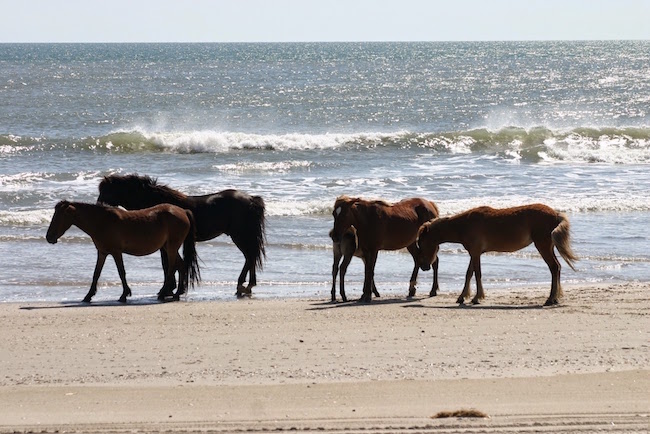
\includegraphics[keepaspectratio]{media/chapter_factors.jpg}}

\begin{quote}
Factors allow us to represent a type of data that exclusive and
categorical. These data may, or may not, be ordered and in most cases,
we can think of these kinds of data to represent things like, treatment
levels, sampling locations, etc.
\end{quote}

\section{Lecture Materials}\label{lecture-materials-4}

\begin{quote}
\textbf{Lecture Slides:} Available interactively in the
\href{https://dyerlabteaching.github.io/Factors/slides.html\#/title-slide}{online
version}
\end{quote}

\begin{figure}[H]

{\centering \pandocbounded{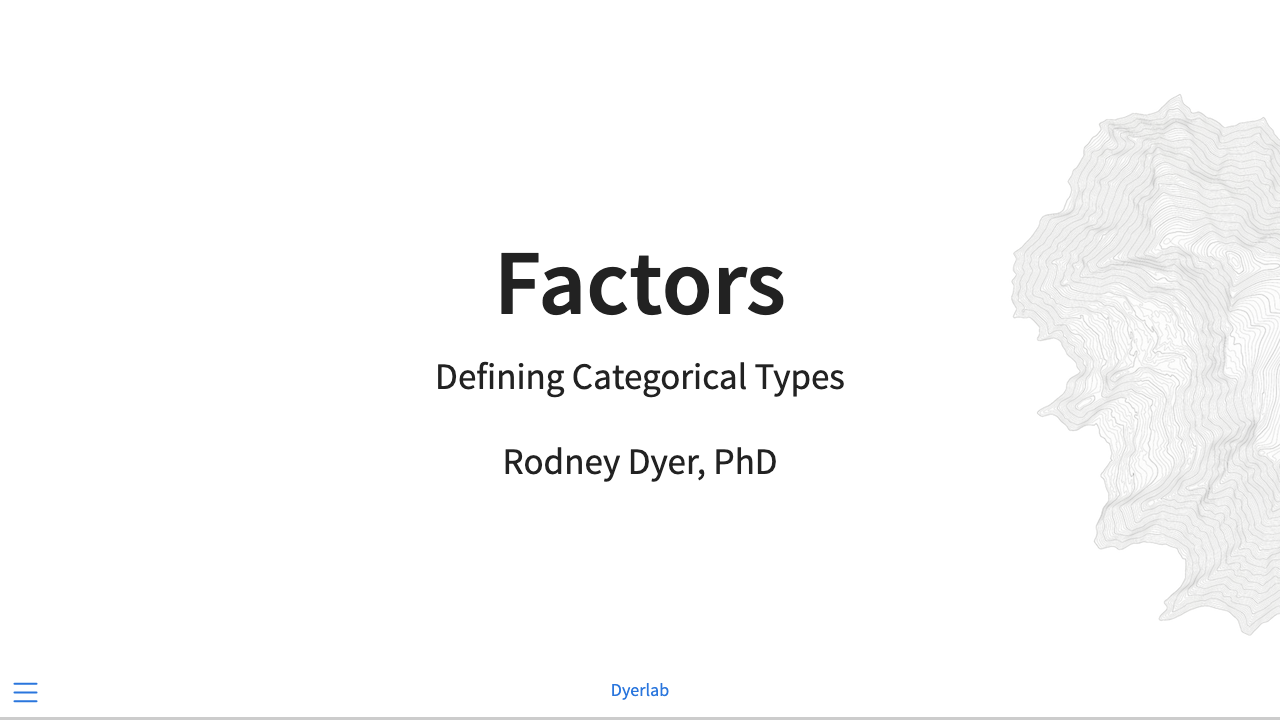
\includegraphics[keepaspectratio]{media/slides_factors.png}}

}

\caption{Lecture Slides}

\end{figure}%

\section{Factors}\label{factors}

I'm going to start with some days of the week because they are
\emph{exclusive} (e.g., you cannot be in both Monday and Wednesday at
the same time). Factors are initially created from string objects,
though you could use \texttt{numeric} data but that would be
\emph{stupid} because you should use things that are descriptive and
strings are much better than that.

\begin{Shaded}
\begin{Highlighting}[]
\NormalTok{weekdays }\OtherTok{\textless{}{-}} \FunctionTok{c}\NormalTok{(}\StringTok{"Monday"}\NormalTok{,}\StringTok{"Tuesday"}\NormalTok{,}\StringTok{"Wednesday"}\NormalTok{,}
              \StringTok{"Thursday"}\NormalTok{,}\StringTok{"Friday"}\NormalTok{,}\StringTok{"Saturday"}\NormalTok{, }
              \StringTok{"Sunday"}\NormalTok{)}
\FunctionTok{class}\NormalTok{( weekdays )}
\end{Highlighting}
\end{Shaded}

\begin{verbatim}
[1] "character"
\end{verbatim}

I'm going to take these days and random sample them to create a vector
of 40 elements. This is something we do all the time and there is a
\texttt{sample()} function that allows us to draw random samples either
with or without replacement (e.g., can you select the same value more
than once).

\begin{Shaded}
\begin{Highlighting}[]
\NormalTok{data }\OtherTok{\textless{}{-}} \FunctionTok{sample}\NormalTok{( weekdays, }\AttributeTok{size=}\DecValTok{40}\NormalTok{, }\AttributeTok{replace=}\ConstantTok{TRUE}\NormalTok{)}
\NormalTok{data}
\end{Highlighting}
\end{Shaded}

\begin{verbatim}
 [1] "Friday"    "Saturday"  "Sunday"    "Saturday"  "Friday"    "Thursday" 
 [7] "Saturday"  "Thursday"  "Monday"    "Sunday"    "Tuesday"   "Wednesday"
[13] "Tuesday"   "Thursday"  "Sunday"    "Saturday"  "Wednesday" "Saturday" 
[19] "Tuesday"   "Friday"    "Sunday"    "Tuesday"   "Sunday"    "Thursday" 
[25] "Saturday"  "Sunday"    "Tuesday"   "Tuesday"   "Friday"    "Monday"   
[31] "Sunday"    "Monday"    "Wednesday" "Monday"    "Saturday"  "Thursday" 
[37] "Saturday"  "Monday"    "Saturday"  "Sunday"   
\end{verbatim}

These data are still

\begin{Shaded}
\begin{Highlighting}[]
\FunctionTok{class}\NormalTok{( data )}
\end{Highlighting}
\end{Shaded}

\begin{verbatim}
[1] "character"
\end{verbatim}

To turn them into a factor, we use\ldots. \texttt{factor()}

\begin{Shaded}
\begin{Highlighting}[]
\NormalTok{days }\OtherTok{\textless{}{-}} \FunctionTok{factor}\NormalTok{( data )}
\FunctionTok{is.factor}\NormalTok{( days )}
\end{Highlighting}
\end{Shaded}

\begin{verbatim}
[1] TRUE
\end{verbatim}

\begin{Shaded}
\begin{Highlighting}[]
\FunctionTok{class}\NormalTok{( days )}
\end{Highlighting}
\end{Shaded}

\begin{verbatim}
[1] "factor"
\end{verbatim}

Now when we look at the data, it looks a lot like it did before
\emph{except for the last line} which shows you the unique levels for
elements in the vector.

\begin{Shaded}
\begin{Highlighting}[]
\NormalTok{days}
\end{Highlighting}
\end{Shaded}

\begin{verbatim}
 [1] Friday    Saturday  Sunday    Saturday  Friday    Thursday  Saturday 
 [8] Thursday  Monday    Sunday    Tuesday   Wednesday Tuesday   Thursday 
[15] Sunday    Saturday  Wednesday Saturday  Tuesday   Friday    Sunday   
[22] Tuesday   Sunday    Thursday  Saturday  Sunday    Tuesday   Tuesday  
[29] Friday    Monday    Sunday    Monday    Wednesday Monday    Saturday 
[36] Thursday  Saturday  Monday    Saturday  Sunday   
Levels: Friday Monday Saturday Sunday Thursday Tuesday Wednesday
\end{verbatim}

\begin{Shaded}
\begin{Highlighting}[]
\FunctionTok{summary}\NormalTok{( days )}
\end{Highlighting}
\end{Shaded}

\begin{verbatim}
   Friday    Monday  Saturday    Sunday  Thursday   Tuesday Wednesday 
        4         5         9         8         5         6         3 
\end{verbatim}

We can put them into data frames and they know how to summarize
themselves properly by counting the number of occurances of each level.

\begin{Shaded}
\begin{Highlighting}[]
\NormalTok{df }\OtherTok{\textless{}{-}} \FunctionTok{data.frame}\NormalTok{( }\AttributeTok{ID =} \DecValTok{1}\SpecialCharTok{:}\DecValTok{40}\NormalTok{, }\AttributeTok{Weekdays =}\NormalTok{ days )}
\FunctionTok{summary}\NormalTok{( df )}
\end{Highlighting}
\end{Shaded}

\begin{verbatim}
       ID             Weekdays
 Min.   : 1.00   Friday   :4  
 1st Qu.:10.75   Monday   :5  
 Median :20.50   Saturday :9  
 Mean   :20.50   Sunday   :8  
 3rd Qu.:30.25   Thursday :5  
 Max.   :40.00   Tuesday  :6  
                 Wednesday:3  
\end{verbatim}

And we can directly access the unique levels

\begin{Shaded}
\begin{Highlighting}[]
\FunctionTok{levels}\NormalTok{( days )}
\end{Highlighting}
\end{Shaded}

\begin{verbatim}
[1] "Friday"    "Monday"    "Saturday"  "Sunday"    "Thursday"  "Tuesday"  
[7] "Wednesday"
\end{verbatim}

So factors can be categorical (e.g., one is just different than the
next) and compared via \texttt{==} and \texttt{!=} values. Or they can
be ordinal such that \texttt{\textgreater{}} and \texttt{\textless{}}
make sense.

By default, a \texttt{factor} is not ordered.

\begin{Shaded}
\begin{Highlighting}[]
\FunctionTok{is.ordered}\NormalTok{( days )}
\end{Highlighting}
\end{Shaded}

\begin{verbatim}
[1] FALSE
\end{verbatim}

\begin{Shaded}
\begin{Highlighting}[]
\NormalTok{days[}\DecValTok{1}\NormalTok{] }\SpecialCharTok{\textless{}}\NormalTok{ days[}\DecValTok{2}\NormalTok{]}
\end{Highlighting}
\end{Shaded}

\begin{verbatim}
Warning in Ops.factor(days[1], days[2]): '<' not meaningful for factors
\end{verbatim}

\begin{verbatim}
[1] NA
\end{verbatim}

\begin{Shaded}
\begin{Highlighting}[]
\NormalTok{data }\OtherTok{\textless{}{-}} \FunctionTok{factor}\NormalTok{( days, }\AttributeTok{ordered=}\ConstantTok{TRUE}\NormalTok{ )}
\NormalTok{data }
\end{Highlighting}
\end{Shaded}

\begin{verbatim}
 [1] Friday    Saturday  Sunday    Saturday  Friday    Thursday  Saturday 
 [8] Thursday  Monday    Sunday    Tuesday   Wednesday Tuesday   Thursday 
[15] Sunday    Saturday  Wednesday Saturday  Tuesday   Friday    Sunday   
[22] Tuesday   Sunday    Thursday  Saturday  Sunday    Tuesday   Tuesday  
[29] Friday    Monday    Sunday    Monday    Wednesday Monday    Saturday 
[36] Thursday  Saturday  Monday    Saturday  Sunday   
7 Levels: Friday < Monday < Saturday < Sunday < Thursday < ... < Wednesday
\end{verbatim}

So that if we go and try to order them, the only way they can be sorted
is alphabetically.

\begin{Shaded}
\begin{Highlighting}[]
\FunctionTok{sort}\NormalTok{( data )}
\end{Highlighting}
\end{Shaded}

\begin{verbatim}
 [1] Friday    Friday    Friday    Friday    Monday    Monday    Monday   
 [8] Monday    Monday    Saturday  Saturday  Saturday  Saturday  Saturday 
[15] Saturday  Saturday  Saturday  Saturday  Sunday    Sunday    Sunday   
[22] Sunday    Sunday    Sunday    Sunday    Sunday    Thursday  Thursday 
[29] Thursday  Thursday  Thursday  Tuesday   Tuesday   Tuesday   Tuesday  
[36] Tuesday   Tuesday   Wednesday Wednesday Wednesday
7 Levels: Friday < Monday < Saturday < Sunday < Thursday < ... < Wednesday
\end{verbatim}

However, this does not make sense. Who in their right mind would like to
have \texttt{Friday} followed immediately by \texttt{Monday}? That is
just not right!

To establish an ordinal variable with a specified sequence of values
that are \emph{not alphabetical} we need to pass along the levels
themselves.

\begin{Shaded}
\begin{Highlighting}[]
\NormalTok{data }\OtherTok{\textless{}{-}} \FunctionTok{factor}\NormalTok{( days, }\AttributeTok{ordered=}\ConstantTok{TRUE}\NormalTok{, }\AttributeTok{levels =}\NormalTok{ weekdays )}
\NormalTok{data}
\end{Highlighting}
\end{Shaded}

\begin{verbatim}
 [1] Friday    Saturday  Sunday    Saturday  Friday    Thursday  Saturday 
 [8] Thursday  Monday    Sunday    Tuesday   Wednesday Tuesday   Thursday 
[15] Sunday    Saturday  Wednesday Saturday  Tuesday   Friday    Sunday   
[22] Tuesday   Sunday    Thursday  Saturday  Sunday    Tuesday   Tuesday  
[29] Friday    Monday    Sunday    Monday    Wednesday Monday    Saturday 
[36] Thursday  Saturday  Monday    Saturday  Sunday   
7 Levels: Monday < Tuesday < Wednesday < Thursday < Friday < ... < Sunday
\end{verbatim}

Now they'll sort properly.

\begin{Shaded}
\begin{Highlighting}[]
\FunctionTok{sort}\NormalTok{( data )}
\end{Highlighting}
\end{Shaded}

\begin{verbatim}
 [1] Monday    Monday    Monday    Monday    Monday    Tuesday   Tuesday  
 [8] Tuesday   Tuesday   Tuesday   Tuesday   Wednesday Wednesday Wednesday
[15] Thursday  Thursday  Thursday  Thursday  Thursday  Friday    Friday   
[22] Friday    Friday    Saturday  Saturday  Saturday  Saturday  Saturday 
[29] Saturday  Saturday  Saturday  Saturday  Sunday    Sunday    Sunday   
[36] Sunday    Sunday    Sunday    Sunday    Sunday   
7 Levels: Monday < Tuesday < Wednesday < Thursday < Friday < ... < Sunday
\end{verbatim}

\subsection{Exclusivity of Factor
Levels}\label{exclusivity-of-factor-levels}

Once you establish a factor, you cannot set the values to anyting that
is outside of the pre-defined levels. If you do, it will just put in
missing data \texttt{NA}.

\begin{Shaded}
\begin{Highlighting}[]
\NormalTok{days[}\DecValTok{3}\NormalTok{] }\OtherTok{\textless{}{-}} \StringTok{"Bob"}
\end{Highlighting}
\end{Shaded}

\begin{verbatim}
Warning in `[<-.factor`(`*tmp*`, 3, value = "Bob"): invalid factor level, NA
generated
\end{verbatim}

\begin{Shaded}
\begin{Highlighting}[]
\NormalTok{days}
\end{Highlighting}
\end{Shaded}

\begin{verbatim}
 [1] Friday    Saturday  <NA>      Saturday  Friday    Thursday  Saturday 
 [8] Thursday  Monday    Sunday    Tuesday   Wednesday Tuesday   Thursday 
[15] Sunday    Saturday  Wednesday Saturday  Tuesday   Friday    Sunday   
[22] Tuesday   Sunday    Thursday  Saturday  Sunday    Tuesday   Tuesday  
[29] Friday    Monday    Sunday    Monday    Wednesday Monday    Saturday 
[36] Thursday  Saturday  Monday    Saturday  Sunday   
Levels: Friday Monday Saturday Sunday Thursday Tuesday Wednesday
\end{verbatim}

That being said, we can have more levels in the factor than observed in
the data. Here is an example of just grabbing the work days from the
week but making the levels equal to all the potential weekdays.

\begin{Shaded}
\begin{Highlighting}[]
\NormalTok{workdays }\OtherTok{\textless{}{-}} \FunctionTok{sample}\NormalTok{( weekdays[}\DecValTok{1}\SpecialCharTok{:}\DecValTok{5}\NormalTok{], }\AttributeTok{size=}\DecValTok{40}\NormalTok{, }\AttributeTok{replace =} \ConstantTok{TRUE}\NormalTok{ )}
\NormalTok{workdays }\OtherTok{\textless{}{-}} \FunctionTok{factor}\NormalTok{( workdays, }\AttributeTok{ordered=}\ConstantTok{TRUE}\NormalTok{, }\AttributeTok{levels =}\NormalTok{ weekdays )}
\end{Highlighting}
\end{Shaded}

And when we summarize it, we see that while it is possible that days may
be named \texttt{Saturday} and \texttt{Sunday}, they are not recoreded
in the data we have for workdays.

\begin{Shaded}
\begin{Highlighting}[]
\FunctionTok{summary}\NormalTok{( workdays )}
\end{Highlighting}
\end{Shaded}

\begin{verbatim}
   Monday   Tuesday Wednesday  Thursday    Friday  Saturday    Sunday 
        7        11         5        10         7         0         0 
\end{verbatim}

We can drop the levels that have no representation

\begin{Shaded}
\begin{Highlighting}[]
\NormalTok{workdays }\OtherTok{\textless{}{-}} \FunctionTok{droplevels}\NormalTok{( workdays ) }
\FunctionTok{summary}\NormalTok{( workdays )}
\end{Highlighting}
\end{Shaded}

\begin{verbatim}
   Monday   Tuesday Wednesday  Thursday    Friday 
        7        11         5        10         7 
\end{verbatim}

\section{\texorpdfstring{The \texttt{forcats}
Library}{The forcats Library}}\label{the-forcats-library}

The \texttt{forcats} library has a bunch of helper functions for working
with factors. This is a relatively small library in \texttt{tidyverse}
but a powerful one. I would recommend looking at the \href{}{cheatsheet}
for it to get a more broad understanding of what functions in this
library can do.

\begin{Shaded}
\begin{Highlighting}[]
\FunctionTok{library}\NormalTok{( forcats )}
\end{Highlighting}
\end{Shaded}

Just like \texttt{stringr} had the \texttt{str\_} prefix, all the
functions here have the \texttt{fct\_} prefix. Here are some examples.

\emph{Counting how many of each factor}

\begin{Shaded}
\begin{Highlighting}[]
\FunctionTok{fct\_count}\NormalTok{( data )}
\end{Highlighting}
\end{Shaded}

\begin{verbatim}
# A tibble: 7 x 2
  f             n
  <ord>     <int>
1 Monday        5
2 Tuesday       6
3 Wednesday     3
4 Thursday      5
5 Friday        4
6 Saturday      9
7 Sunday        8
\end{verbatim}

\emph{Lumping Rare Factors}

\begin{Shaded}
\begin{Highlighting}[]
\NormalTok{lumped }\OtherTok{\textless{}{-}} \FunctionTok{fct\_lump\_min}\NormalTok{( data, }\AttributeTok{min =} \DecValTok{5}\NormalTok{ )}
\FunctionTok{fct\_count}\NormalTok{( lumped )}
\end{Highlighting}
\end{Shaded}

\begin{verbatim}
# A tibble: 6 x 2
  f            n
  <ord>    <int>
1 Monday       5
2 Tuesday      6
3 Thursday     5
4 Saturday     9
5 Sunday       8
6 Other        7
\end{verbatim}

\emph{Reordering Factor Levels by Frequency}

\begin{Shaded}
\begin{Highlighting}[]
\NormalTok{freq }\OtherTok{\textless{}{-}} \FunctionTok{fct\_infreq}\NormalTok{( data )}
\FunctionTok{levels}\NormalTok{( freq )}
\end{Highlighting}
\end{Shaded}

\begin{verbatim}
[1] "Saturday"  "Sunday"    "Tuesday"   "Monday"    "Thursday"  "Friday"   
[7] "Wednesday"
\end{verbatim}

\emph{Reordering by Order of Appearance}

\begin{Shaded}
\begin{Highlighting}[]
\NormalTok{ordered }\OtherTok{\textless{}{-}} \FunctionTok{fct\_inorder}\NormalTok{( data )}
\FunctionTok{levels}\NormalTok{( ordered )}
\end{Highlighting}
\end{Shaded}

\begin{verbatim}
[1] "Friday"    "Saturday"  "Sunday"    "Thursday"  "Monday"    "Tuesday"  
[7] "Wednesday"
\end{verbatim}

\emph{Reordering Specific Levels}

\begin{Shaded}
\begin{Highlighting}[]
\NormalTok{newWeek }\OtherTok{\textless{}{-}} \FunctionTok{fct\_relevel}\NormalTok{( data, }\StringTok{"Sunday"}\NormalTok{)}
\FunctionTok{levels}\NormalTok{( newWeek )}
\end{Highlighting}
\end{Shaded}

\begin{verbatim}
[1] "Sunday"    "Monday"    "Tuesday"   "Wednesday" "Thursday"  "Friday"   
[7] "Saturday" 
\end{verbatim}

\emph{Dropping Unobserved Levels} - just like \texttt{droplevels()}

\begin{Shaded}
\begin{Highlighting}[]
\NormalTok{dropped }\OtherTok{\textless{}{-}} \FunctionTok{fct\_drop}\NormalTok{( workdays )}
\FunctionTok{summary}\NormalTok{( dropped )}
\end{Highlighting}
\end{Shaded}

\begin{verbatim}
   Monday   Tuesday Wednesday  Thursday    Friday 
        7        11         5        10         7 
\end{verbatim}

\section{Using Factors}\label{using-factors}

It is common to use factors as an organizing princple in our data. For
example, let's say we went out and sampled three different species of
plants and measured characteristics of their flower size. The
\texttt{iris} data set from R.A. Fisher is a classid data set that is
include in \texttt{R} and it looks like this (the functions
\texttt{head()} and \texttt{tail()} show the top or bottom parts of a
data frame).

\begin{Shaded}
\begin{Highlighting}[]
\FunctionTok{head}\NormalTok{(iris)}
\end{Highlighting}
\end{Shaded}

\begin{verbatim}
  Sepal.Length Sepal.Width Petal.Length Petal.Width Species
1          5.1         3.5          1.4         0.2  setosa
2          4.9         3.0          1.4         0.2  setosa
3          4.7         3.2          1.3         0.2  setosa
4          4.6         3.1          1.5         0.2  setosa
5          5.0         3.6          1.4         0.2  setosa
6          5.4         3.9          1.7         0.4  setosa
\end{verbatim}

By default it is a \texttt{data.frame} object.

\begin{Shaded}
\begin{Highlighting}[]
\FunctionTok{class}\NormalTok{( iris )}
\end{Highlighting}
\end{Shaded}

\begin{verbatim}
[1] "data.frame"
\end{verbatim}

\subsection{By the by}\label{by-the-by}

One helpful function in base \texttt{R} is the \texttt{by()} function.
It has the following form.

\begin{verbatim}
by( data, index, function)
\end{verbatim}

The \texttt{data} is the raw data you are using, the \texttt{index} is a
vector that we are using to differentiate among the species (the
factor), and the function is what function we want to use.

So for example, if I were interesed in the mean length of the Sepal for
each species, I could write.

\begin{Shaded}
\begin{Highlighting}[]
\NormalTok{meanSepalLength }\OtherTok{\textless{}{-}} \FunctionTok{by}\NormalTok{( iris}\SpecialCharTok{$}\NormalTok{Sepal.Length, iris}\SpecialCharTok{$}\NormalTok{Species, mean )}
\FunctionTok{class}\NormalTok{( meanSepalLength )}
\end{Highlighting}
\end{Shaded}

\begin{verbatim}
[1] "by"
\end{verbatim}

\begin{Shaded}
\begin{Highlighting}[]
\NormalTok{meanSepalLength}
\end{Highlighting}
\end{Shaded}

\begin{verbatim}
iris$Species: setosa
[1] 5.006
------------------------------------------------------------ 
iris$Species: versicolor
[1] 5.936
------------------------------------------------------------ 
iris$Species: virginica
[1] 6.588
\end{verbatim}

I could also do the same thing with the variance in sepal length.

\begin{Shaded}
\begin{Highlighting}[]
\FunctionTok{by}\NormalTok{( iris[,}\DecValTok{2}\NormalTok{], iris[,}\DecValTok{5}\NormalTok{], var ) }\OtherTok{{-}\textgreater{}}\NormalTok{ varSepalLength}
\NormalTok{varSepalLength }
\end{Highlighting}
\end{Shaded}

\begin{verbatim}
iris[, 5]: setosa
[1] 0.1436898
------------------------------------------------------------ 
iris[, 5]: versicolor
[1] 0.09846939
------------------------------------------------------------ 
iris[, 5]: virginica
[1] 0.1040041
\end{verbatim}

Using these kinds of functions we can create a summary data frame.

\begin{Shaded}
\begin{Highlighting}[]
\FunctionTok{library}\NormalTok{( tidyverse )}
\end{Highlighting}
\end{Shaded}

\begin{verbatim}
-- Attaching core tidyverse packages ------------------------ tidyverse 2.0.0 --
v dplyr     1.2.1     v readr     2.2.0
v ggplot2   4.0.2     v stringr   1.6.0
v lubridate 1.9.5     v tibble    3.3.1
v purrr     1.2.1     v tidyr     1.3.2
-- Conflicts ------------------------------------------ tidyverse_conflicts() --
x dplyr::filter() masks stats::filter()
x dplyr::lag()    masks stats::lag()
i Use the conflicted package (<http://conflicted.r-lib.org/>) to force all conflicts to become errors
\end{verbatim}

\begin{Shaded}
\begin{Highlighting}[]
\NormalTok{df }\OtherTok{\textless{}{-}} \FunctionTok{tibble}\NormalTok{( }\AttributeTok{Species =} \FunctionTok{levels}\NormalTok{( iris}\SpecialCharTok{$}\NormalTok{Species), }
              \AttributeTok{Average =}\NormalTok{ meanSepalLength,}
              \AttributeTok{Variance =}\NormalTok{ varSepalLength}
\NormalTok{)}
\NormalTok{df}
\end{Highlighting}
\end{Shaded}

\begin{verbatim}
# A tibble: 3 x 3
  Species    Average  Variance  
  <chr>      <by[1d]> <by[1d]>  
1 setosa     5.006    0.14368980
2 versicolor 5.936    0.09846939
3 virginica  6.588    0.10400408
\end{verbatim}

\section{Missing Data}\label{missing-data-1}

Missing data is a .red{[}fact of life{]} and \texttt{R} is very
opinionated about how it handles missing values. In general, missing
data is encoded as \texttt{NA} and is a valid entry for any data type
(character, numeric, logical, factor, etc.). Where this becomes tricky
is when we are doing operations on data that has missing values.
\texttt{R} could take two routes:

\begin{enumerate}
\def\labelenumi{\arabic{enumi}.}
\tightlist
\item
  It could ignore the data and give you the answer directly as if the
  data were not missing, or\\
\item
  It could let you know that there is missing data and make you do
  something about it.
\end{enumerate}

Fortunately, \texttt{R} took the second route.

An example from the iris data, I'm going to add some missing data to it.

\begin{Shaded}
\begin{Highlighting}[]
\NormalTok{missingIris }\OtherTok{\textless{}{-}}\NormalTok{ iris[, }\DecValTok{4}\SpecialCharTok{:}\DecValTok{5}\NormalTok{]}
\NormalTok{missingIris}\SpecialCharTok{$}\NormalTok{Petal.Width[ }\FunctionTok{c}\NormalTok{(}\DecValTok{2}\NormalTok{,}\DecValTok{6}\NormalTok{,}\DecValTok{12}\NormalTok{) ] }\OtherTok{\textless{}{-}} \ConstantTok{NA}
\FunctionTok{summary}\NormalTok{( missingIris )}
\end{Highlighting}
\end{Shaded}

\begin{verbatim}
  Petal.Width          Species  
 Min.   :0.100   setosa    :50  
 1st Qu.:0.300   versicolor:50  
 Median :1.300   virginica :50  
 Mean   :1.218                  
 3rd Qu.:1.800                  
 Max.   :2.500                  
 NA's   :3                      
\end{verbatim}

Notice how the missing data is denoted in the summary.

\subsection{Indications of Missing
Data}\label{indications-of-missing-data}

When we perform a mathematical or statistical operation on data that has
missing elements \texttt{R} will \textbf{always} return NA as the
result.

\begin{Shaded}
\begin{Highlighting}[]
\FunctionTok{mean}\NormalTok{( missingIris}\SpecialCharTok{$}\NormalTok{Petal.Width )}
\end{Highlighting}
\end{Shaded}

\begin{verbatim}
[1] NA
\end{verbatim}

This warns you that .red{[}at least one{]} of the observations in the
data is missing.

Same output for using \texttt{by()}, it will put \texttt{NA} into each
level that has at least one missing value.

\begin{Shaded}
\begin{Highlighting}[]
\FunctionTok{by}\NormalTok{( missingIris}\SpecialCharTok{$}\NormalTok{Petal.Width, missingIris}\SpecialCharTok{$}\NormalTok{Species, mean )}
\end{Highlighting}
\end{Shaded}

\begin{verbatim}
missingIris$Species: setosa
[1] NA
------------------------------------------------------------ 
missingIris$Species: versicolor
[1] 1.326
------------------------------------------------------------ 
missingIris$Species: virginica
[1] 2.026
\end{verbatim}

\subsection{Working with Missing Data}\label{working-with-missing-data}

To acknowledge that there are missing data and you still want the
values, you need to tell the function you are using that data is missing
and you are OK with that using the optional argument \texttt{na.rm=TRUE}
(\texttt{na} = missing data \& \texttt{rm} is \emph{remove}).

\begin{Shaded}
\begin{Highlighting}[]
\FunctionTok{mean}\NormalTok{( missingIris}\SpecialCharTok{$}\NormalTok{Petal.Width, }\AttributeTok{na.rm=}\ConstantTok{TRUE}\NormalTok{)}
\end{Highlighting}
\end{Shaded}

\begin{verbatim}
[1] 1.218367
\end{verbatim}

To pass this to the \texttt{by()} function, we add the optional argument
\texttt{na.rm=TRUE} and \texttt{by()} passes it along to the
\texttt{mean} function as ``\ldots{}''

\begin{Shaded}
\begin{Highlighting}[]
\FunctionTok{by}\NormalTok{( missingIris}\SpecialCharTok{$}\NormalTok{Petal.Width, missingIris}\SpecialCharTok{$}\NormalTok{Species, mean, }\AttributeTok{na.rm=}\ConstantTok{TRUE}\NormalTok{ )}
\end{Highlighting}
\end{Shaded}

\begin{verbatim}
missingIris$Species: setosa
[1] 0.2446809
------------------------------------------------------------ 
missingIris$Species: versicolor
[1] 1.326
------------------------------------------------------------ 
missingIris$Species: virginica
[1] 2.026
\end{verbatim}

\section{Fancy Tables}\label{fancy-tables}

Making data frames like that above is a \emph{classic} maneuver in
\texttt{R} and I'm going to use this to introduce the use of the
\texttt{knitr} library to show you how to take a set of data and turn it
into a table for your manuscript.

\begin{Shaded}
\begin{Highlighting}[]
\FunctionTok{library}\NormalTok{( knitr )}
\end{Highlighting}
\end{Shaded}

Now we can make a table as:

\begin{Shaded}
\begin{Highlighting}[]
\FunctionTok{kable}\NormalTok{( df )}
\end{Highlighting}
\end{Shaded}

{\def\LTcaptype{none} % do not increment counter
\begin{longtable}[]{@{}lrr@{}}
\toprule\noalign{}
Species & Average & Variance \\
\midrule\noalign{}
\endhead
\bottomrule\noalign{}
\endlastfoot
setosa & 5.006 & 0.14368980 \\
versicolor & 5.936 & 0.09846939 \\
virginica & 6.588 & 0.10400408 \\
\end{longtable}
}

We can even add a caption to it.

\begin{Shaded}
\begin{Highlighting}[]
\NormalTok{irisTable }\OtherTok{\textless{}{-}} \FunctionTok{kable}\NormalTok{( df, }\AttributeTok{caption =} \StringTok{"The mean and variance in measured sepal length (in cm) for three species of Iris."}\NormalTok{)}
\NormalTok{irisTable}
\end{Highlighting}
\end{Shaded}

\begin{longtable}[]{@{}lrr@{}}
\caption{The mean and variance in measured sepal length (in cm) for
three species of Iris.}\tabularnewline
\toprule\noalign{}
Species & Average & Variance \\
\midrule\noalign{}
\endfirsthead
\toprule\noalign{}
Species & Average & Variance \\
\midrule\noalign{}
\endhead
\bottomrule\noalign{}
\endlastfoot
setosa & 5.006 & 0.14368980 \\
versicolor & 5.936 & 0.09846939 \\
virginica & 6.588 & 0.10400408 \\
\end{longtable}

In addition to this basic library, there is an \texttt{kableExtra} one
that allows us to get even more fancy. You must go check out
\href{https://cran.r-project.org/web/packages/kableExtra/vignettes/awesome_table_in_html.html}{this}
webpage (which is an RMarkdown page by the way) to see all the other
ways you can fancy up your tables.

\begin{Shaded}
\begin{Highlighting}[]
\FunctionTok{library}\NormalTok{( kableExtra )}
\end{Highlighting}
\end{Shaded}

\begin{verbatim}

Attaching package: 'kableExtra'
\end{verbatim}

\begin{verbatim}
The following object is masked from 'package:dplyr':

    group_rows
\end{verbatim}

\subsection{Table Themes}\label{table-themes}

Here are some examples Themes

\begin{Shaded}
\begin{Highlighting}[]
\FunctionTok{kable\_paper}\NormalTok{( irisTable )}
\end{Highlighting}
\end{Shaded}

\begin{longtable}[t]{lrr}
\caption{\label{tab:unnamed-chunk-38}The mean and variance in measured sepal length (in cm) for three species of Iris.}\\
\toprule
Species & Average & Variance\\
\midrule
setosa & 5.006 & 0.14368980\\
versicolor & 5.936 & 0.09846939\\
virginica & 6.588 & 0.10400408\\
\bottomrule
\end{longtable}

\begin{Shaded}
\begin{Highlighting}[]
\FunctionTok{kable\_classic}\NormalTok{( irisTable )}
\end{Highlighting}
\end{Shaded}

\begin{longtable}[t]{lrr}
\caption{\label{tab:unnamed-chunk-39}The mean and variance in measured sepal length (in cm) for three species of Iris.}\\
\toprule
Species & Average & Variance\\
\midrule
setosa & 5.006 & 0.14368980\\
versicolor & 5.936 & 0.09846939\\
virginica & 6.588 & 0.10400408\\
\bottomrule
\end{longtable}

\begin{Shaded}
\begin{Highlighting}[]
\FunctionTok{kable\_classic\_2}\NormalTok{( irisTable )}
\end{Highlighting}
\end{Shaded}

\begin{longtable}[t]{lrr}
\caption{\label{tab:unnamed-chunk-40}The mean and variance in measured sepal length (in cm) for three species of Iris.}\\
\toprule
Species & Average & Variance\\
\midrule
setosa & 5.006 & 0.14368980\\
versicolor & 5.936 & 0.09846939\\
virginica & 6.588 & 0.10400408\\
\bottomrule
\end{longtable}

\begin{Shaded}
\begin{Highlighting}[]
\FunctionTok{kable\_minimal}\NormalTok{( irisTable )}
\end{Highlighting}
\end{Shaded}

\begin{longtable}[t]{lrr}
\caption{\label{tab:unnamed-chunk-41}The mean and variance in measured sepal length (in cm) for three species of Iris.}\\
\toprule
Species & Average & Variance\\
\midrule
setosa & 5.006 & 0.14368980\\
versicolor & 5.936 & 0.09846939\\
virginica & 6.588 & 0.10400408\\
\bottomrule
\end{longtable}

\begin{Shaded}
\begin{Highlighting}[]
\FunctionTok{kable\_material}\NormalTok{( irisTable,}\AttributeTok{lightable\_options =} \FunctionTok{c}\NormalTok{(}\StringTok{"striped"}\NormalTok{, }\StringTok{"hover"}\NormalTok{) )}
\end{Highlighting}
\end{Shaded}

\begin{longtable}[t]{lrr}
\caption{\label{tab:unnamed-chunk-42}The mean and variance in measured sepal length (in cm) for three species of Iris.}\\
\toprule
Species & Average & Variance\\
\midrule
setosa & 5.006 & 0.14368980\\
versicolor & 5.936 & 0.09846939\\
virginica & 6.588 & 0.10400408\\
\bottomrule
\end{longtable}

\begin{Shaded}
\begin{Highlighting}[]
\FunctionTok{kable\_material\_dark}\NormalTok{( irisTable )}
\end{Highlighting}
\end{Shaded}

\begin{longtable}[t]{lrr}
\caption{\label{tab:unnamed-chunk-43}The mean and variance in measured sepal length (in cm) for three species of Iris.}\\
\toprule
Species & Average & Variance\\
\midrule
setosa & 5.006 & 0.14368980\\
versicolor & 5.936 & 0.09846939\\
virginica & 6.588 & 0.10400408\\
\bottomrule
\end{longtable}

\subsection{Table Sizes and Positions}\label{table-sizes-and-positions}

We can be specific about the size and location of the whole table.

\begin{Shaded}
\begin{Highlighting}[]
\FunctionTok{kable\_paper}\NormalTok{(irisTable, }\AttributeTok{full\_width =} \ConstantTok{FALSE}\NormalTok{ )}
\end{Highlighting}
\end{Shaded}

\begin{longtable}[t]{lrr}
\caption{\label{tab:unnamed-chunk-44}The mean and variance in measured sepal length (in cm) for three species of Iris.}\\
\toprule
Species & Average & Variance\\
\midrule
setosa & 5.006 & 0.14368980\\
versicolor & 5.936 & 0.09846939\\
virginica & 6.588 & 0.10400408\\
\bottomrule
\end{longtable}

\subsection{Heading Judo}\label{heading-judo}

We can do some really cool stuff on row and column headings. Here is an
example where I add another row above the data columns for output.

\begin{Shaded}
\begin{Highlighting}[]
\NormalTok{classic }\OtherTok{\textless{}{-}} \FunctionTok{kable\_paper}\NormalTok{( irisTable )}
\FunctionTok{add\_header\_above}\NormalTok{( classic, }\FunctionTok{c}\NormalTok{(}\StringTok{" "} \OtherTok{=} \DecValTok{1}\NormalTok{, }\StringTok{"Sepal Length (cm)"} \OtherTok{=} \DecValTok{2}\NormalTok{))}
\end{Highlighting}
\end{Shaded}

\begin{longtable}[t]{lrr}
\caption{\label{tab:unnamed-chunk-45}The mean and variance in measured sepal length (in cm) for three species of Iris.}\\
\toprule
\multicolumn{1}{c}{ } & \multicolumn{2}{c}{Sepal Length (cm)} \\
\cmidrule(l{3pt}r{3pt}){2-3}
Species & Average & Variance\\
\midrule
setosa & 5.006 & 0.14368980\\
versicolor & 5.936 & 0.09846939\\
virginica & 6.588 & 0.10400408\\
\bottomrule
\end{longtable}

\chapter{Joins}\label{joins}

\pandocbounded{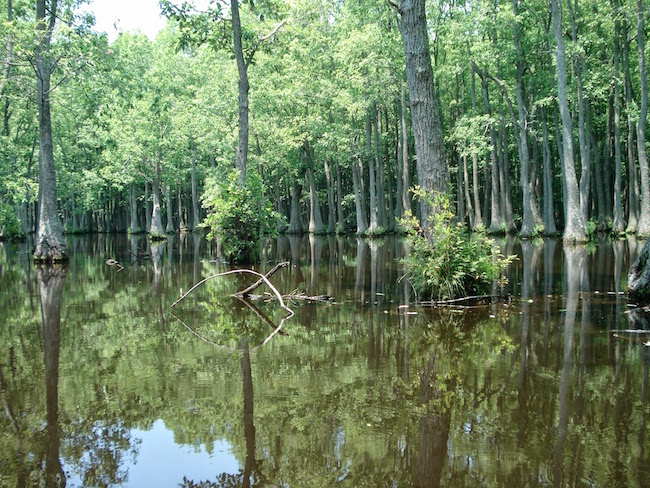
\includegraphics[keepaspectratio]{media/chapter_joins.jpg}}

\begin{quote}
Effectively storing data often requires the use of several data frames
to reduce redundancy. In this short chapter, we will cover how to join
data from multiple sources.
\end{quote}

\section{Lecture Materials}\label{lecture-materials-5}

\begin{quote}
\textbf{Lecture Slides:} Available interactively in the
\href{https://dyerlabteaching.github.io/Joins/slides.html\#/title-slide}{online
version}
\end{quote}

\begin{figure}[H]

{\centering \pandocbounded{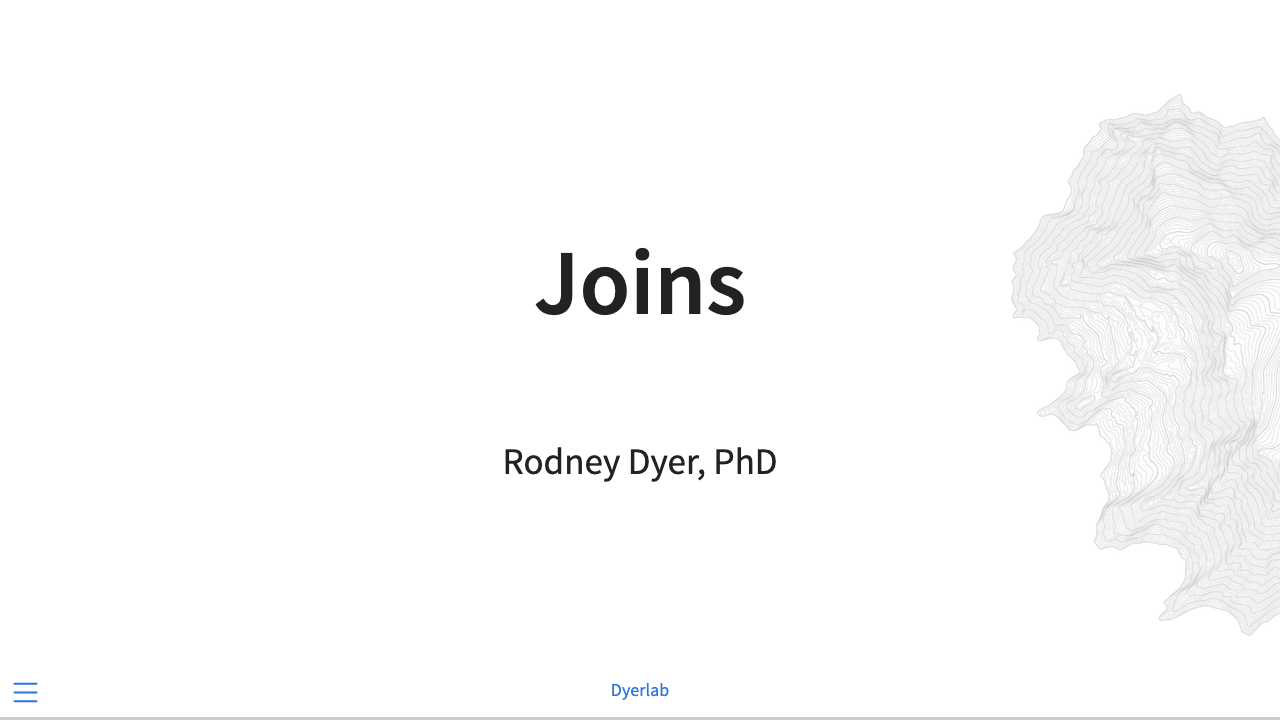
\includegraphics[keepaspectratio]{media/slides_joins.png}}

}

\caption{Lecture Slides}

\end{figure}%

Rarely do we work on only one \texttt{data.frame}, particularly when we
start working with complex data and data contained within relational
databases. In these cases, data are factored into several tables (akin
to \texttt{data.frame} objects) with entries that connect the
information from one table to another. Consider the following example
tables

\begin{figure}[H]

{\centering \pandocbounded{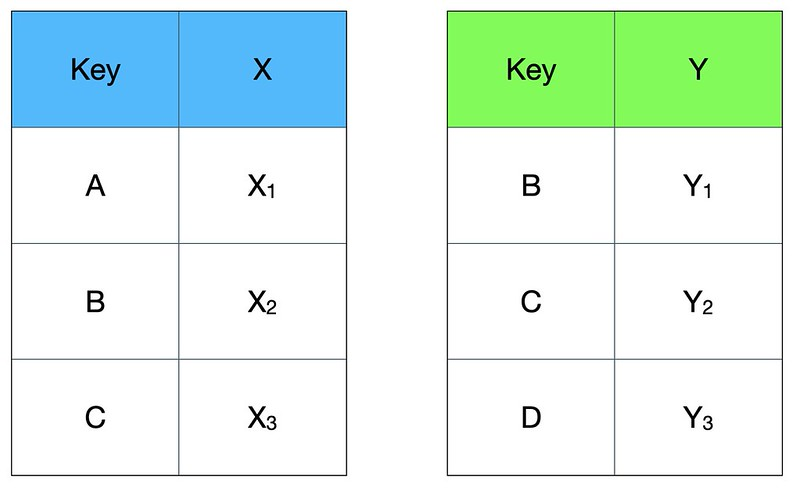
\includegraphics[keepaspectratio]{media/data_table_structure.jpg}}

}

\caption{Example data table structure}

\end{figure}%

Each has a column I named \emph{Key} and another with some data in it.
In \texttt{R} they could be defined as:

\begin{Shaded}
\begin{Highlighting}[]
\NormalTok{df.X }\OtherTok{\textless{}{-}} \FunctionTok{data.frame}\NormalTok{( }\AttributeTok{Key =} \FunctionTok{c}\NormalTok{(}\StringTok{"A"}\NormalTok{,}\StringTok{"B"}\NormalTok{,}\StringTok{"C"}\NormalTok{),}
                    \AttributeTok{X =} \FunctionTok{c}\NormalTok{(}\DecValTok{1}\NormalTok{,}\DecValTok{2}\NormalTok{,}\DecValTok{3}\NormalTok{) )}
\NormalTok{df.X}
\end{Highlighting}
\end{Shaded}

\begin{verbatim}
  Key X
1   A 1
2   B 2
3   C 3
\end{verbatim}

and

\begin{Shaded}
\begin{Highlighting}[]
\NormalTok{df.Y }\OtherTok{\textless{}{-}} \FunctionTok{data.frame}\NormalTok{( }\AttributeTok{Key =} \FunctionTok{c}\NormalTok{(}\StringTok{"B"}\NormalTok{,}\StringTok{"C"}\NormalTok{,}\StringTok{"D"}\NormalTok{),}
                    \AttributeTok{Y =} \FunctionTok{c}\NormalTok{(}\DecValTok{10}\NormalTok{,}\DecValTok{11}\NormalTok{,}\DecValTok{12}\NormalTok{) )}
\NormalTok{df.Y}
\end{Highlighting}
\end{Shaded}

\begin{verbatim}
  Key  Y
1   B 10
2   C 11
3   D 12
\end{verbatim}

\section{Keys}\label{keys}

An important component of relational data are the \emph{keys}. These are
unique identifiers for a particular datum from a table. In each of these
examples the variable (obviously named) \texttt{Key} is what is called a
\emph{Primary Key} because it uniquely identifies each row. You can
verify this by counting the number of entries then filtering only for
ones with 2 or more instances.

\begin{Shaded}
\begin{Highlighting}[]
\FunctionTok{library}\NormalTok{( tidyverse )}
\end{Highlighting}
\end{Shaded}

\begin{verbatim}
-- Attaching core tidyverse packages ------------------------ tidyverse 2.0.0 --
v dplyr     1.2.1     v readr     2.2.0
v forcats   1.0.1     v stringr   1.6.0
v ggplot2   4.0.2     v tibble    3.3.1
v lubridate 1.9.5     v tidyr     1.3.2
v purrr     1.2.1     
-- Conflicts ------------------------------------------ tidyverse_conflicts() --
x dplyr::filter() masks stats::filter()
x dplyr::lag()    masks stats::lag()
i Use the conflicted package (<http://conflicted.r-lib.org/>) to force all conflicts to become errors
\end{verbatim}

\begin{Shaded}
\begin{Highlighting}[]
\NormalTok{df.X }\SpecialCharTok{\%\textgreater{}\%}
  \FunctionTok{count}\NormalTok{( Key ) }\SpecialCharTok{\%\textgreater{}\%}
  \FunctionTok{filter}\NormalTok{( n }\SpecialCharTok{\textgreater{}} \DecValTok{1}\NormalTok{ )}
\end{Highlighting}
\end{Shaded}

\begin{verbatim}
[1] Key n  
<0 rows> (or 0-length row.names)
\end{verbatim}

Notice there is nothing here as each is unique.

\begin{quote}
The column \texttt{Key} is a Primary Key for the \texttt{df.X} data
because it identifies a unique row \emph{in that table}. In addition to
a \emph{Primary Key} we can have a \emph{Foreign Key} when it is used to
indicate data within a separate table. For example, if I am interested
to see if the smallest value in \texttt{df.X\$X} corresponds with the
smallest value in \texttt{df.Y\$Y}, then I will be using the
\texttt{Key} form \texttt{df.X} representing \texttt{max(X)} to find the
value of \texttt{Y} in \texttt{df.Y} and evaluate if it is
\texttt{max(Y)}. This means that \texttt{df.X\$Key} is a \emph{Foreign
Key} as it points to a row in the \texttt{df.Y} data frame.
\end{quote}

The keys are used to link together different tables.

\section{Joins}\label{joins-1}

\begin{quote}
A \emph{join} is where we combine information contained within two data
frames.\\
Joins are ways to merge together data and come in four flavors.
\end{quote}

\subsection{Left Join}\label{left-join}

A \emph{left join} is one where all the data from the left data frame is
in the result and the data whose keys in the right data frame are
present in the left one are also included. Graphically, this leads to:

\begin{figure}[H]

{\centering \pandocbounded{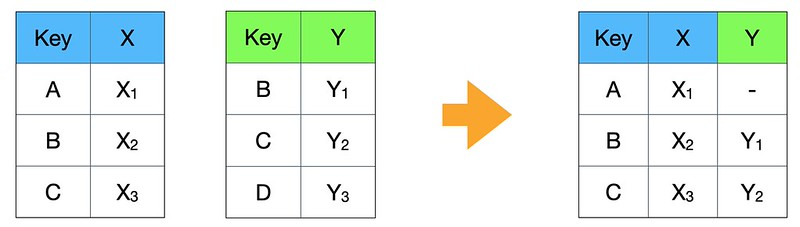
\includegraphics[keepaspectratio]{media/left_join.jpg}}

}

\caption{left join}

\end{figure}%

Where in \texttt{R} we do this using the \texttt{left\_join()} function.

\begin{Shaded}
\begin{Highlighting}[]
\NormalTok{df.X }\SpecialCharTok{\%\textgreater{}\%}
  \FunctionTok{left\_join}\NormalTok{( df.Y, }\AttributeTok{by=}\StringTok{"Key"}\NormalTok{)}
\end{Highlighting}
\end{Shaded}

\begin{verbatim}
  Key X  Y
1   A 1 NA
2   B 2 10
3   C 3 11
\end{verbatim}

\subsection{Right Join}\label{right-join}

The right join does the same thing but keeps all the keys in the right
data table and has missing data where the key in the left one is not in
the right one.

\begin{figure}[H]

{\centering \pandocbounded{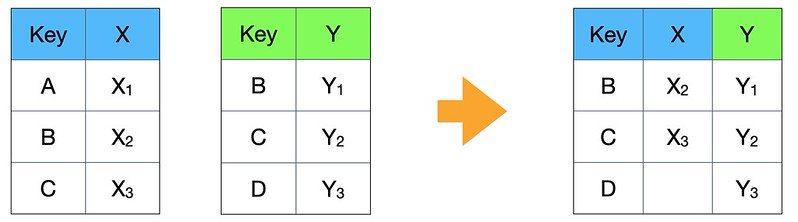
\includegraphics[keepaspectratio]{media/right_join.jpg}}

}

\caption{Right Join}

\end{figure}%

This is accomplished using the \texttt{right\_join()} function.

\begin{Shaded}
\begin{Highlighting}[]
\NormalTok{df.X }\SpecialCharTok{\%\textgreater{}\%}
  \FunctionTok{right\_join}\NormalTok{( df.Y, }\AttributeTok{by=}\StringTok{"Key"}\NormalTok{)}
\end{Highlighting}
\end{Shaded}

\begin{verbatim}
  Key  X  Y
1   B  2 10
2   C  3 11
3   D NA 12
\end{verbatim}

\subsection{Full (or Outer) Join}\label{full-or-outer-join}

This join is one where all the keys are retained adding missing data as
necessary.

\begin{figure}[H]

{\centering \pandocbounded{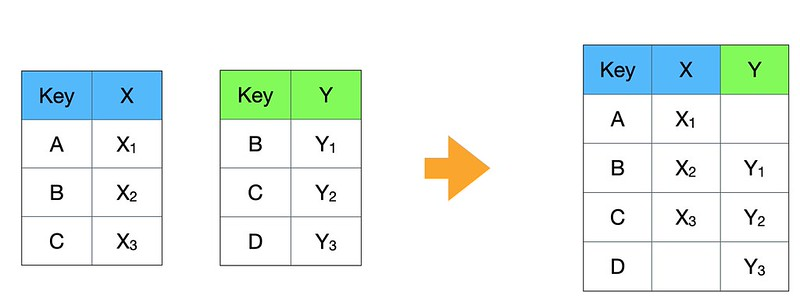
\includegraphics[keepaspectratio]{media/outer_join.jpg}}

}

\caption{Outer Join}

\end{figure}%

\begin{Shaded}
\begin{Highlighting}[]
\NormalTok{df.X }\SpecialCharTok{\%\textgreater{}\%}
  \FunctionTok{full\_join}\NormalTok{( df.Y, }\AttributeTok{by=}\StringTok{"Key"}\NormalTok{)}
\end{Highlighting}
\end{Shaded}

\begin{verbatim}
  Key  X  Y
1   A  1 NA
2   B  2 10
3   C  3 11
4   D NA 12
\end{verbatim}

\subsection{Inner Join}\label{inner-join}

The last one retains \emph{only} those keys that are common in both.

\begin{figure}[H]

{\centering \pandocbounded{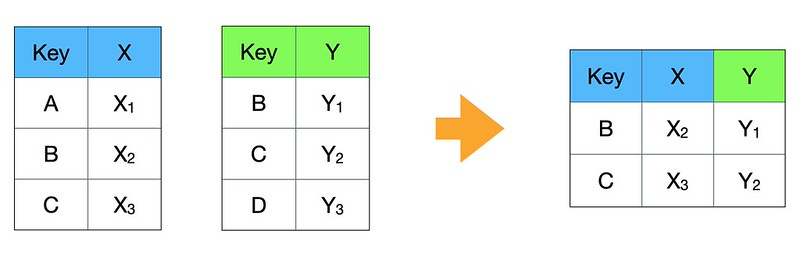
\includegraphics[keepaspectratio]{media/inner_join.jpg}}

}

\caption{Inner Join}

\end{figure}%

\begin{Shaded}
\begin{Highlighting}[]
\NormalTok{df.X }\SpecialCharTok{\%\textgreater{}\%}
  \FunctionTok{inner\_join}\NormalTok{( df.Y, }\AttributeTok{by=}\StringTok{"Key"}\NormalTok{)}
\end{Highlighting}
\end{Shaded}

\begin{verbatim}
  Key X  Y
1   B 2 10
2   C 3 11
\end{verbatim}

\subsection{Filtering Joins}\label{filtering-joins}

We can also use joins to filter values within one \texttt{data.frame}.
Here the \texttt{semi\_join()} keeps everything in the left data that
has a key in the right one, but \textbf{importantly} it does not import
the right data columns into the result.

\begin{Shaded}
\begin{Highlighting}[]
\NormalTok{df.X }\SpecialCharTok{\%\textgreater{}\%}
  \FunctionTok{semi\_join}\NormalTok{( df.Y )}
\end{Highlighting}
\end{Shaded}

\begin{verbatim}
Joining with `by = join_by(Key)`
\end{verbatim}

\begin{verbatim}
  Key X
1   B 2
2   C 3
\end{verbatim}

The opposite of this is the \texttt{anti\_join()} which drops everything
in the left table that has a key in the right one, leaving only the ones
that are unique.

\begin{Shaded}
\begin{Highlighting}[]
\NormalTok{df.X }\SpecialCharTok{\%\textgreater{}\%}
  \FunctionTok{anti\_join}\NormalTok{( df.Y )}
\end{Highlighting}
\end{Shaded}

\begin{verbatim}
Joining with `by = join_by(Key)`
\end{verbatim}

\begin{verbatim}
  Key X
1   A 1
\end{verbatim}

\chapter{Data Visualization}\label{data-visualization}

\pandocbounded{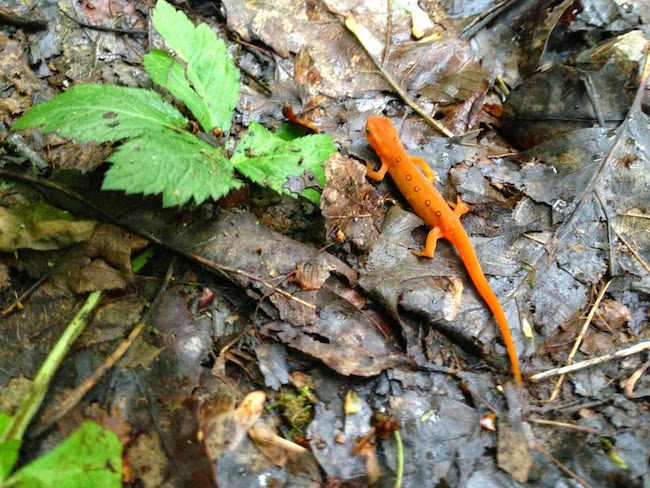
\includegraphics[keepaspectratio]{media/chapter_classic.jpg}}

\begin{quote}
Visualization gives you answers to questions you didn't know you had.
\end{quote}

\section{Lecture Materials}\label{lecture-materials-6}

\begin{quote}
\textbf{Lecture Slides:} Available interactively in the
\href{https://dyerlabteaching.github.io/Graphics-That-Do-Not-Suck/slides_classic.html\#/title-slide}{online
version}
\end{quote}

\begin{figure}[H]

{\centering \pandocbounded{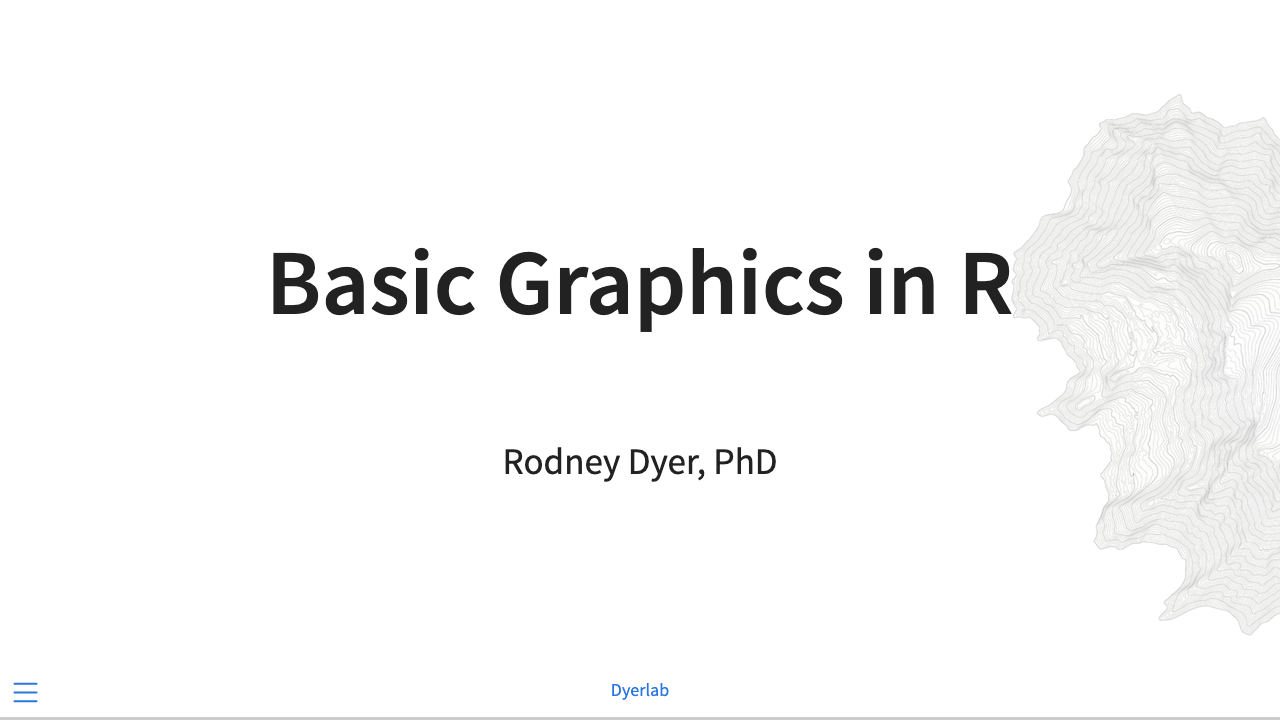
\includegraphics[keepaspectratio]{media/slides_classic.png}}

}

\caption{Lecture Slides}

\end{figure}%

\section{The Data}\label{the-data-1}

The \texttt{iris} flower data set (also known as \emph{Fisher's Iris
data set}) is a multivariate data set introduced by the British
statistician, eugenicist, and biologist
\href{https://en.wikipedia.org/wiki/Ronald_Fisher}{Ronald Fisher} in his
\href{https://onlinelibrary.wiley.com/doi/abs/10.1111/j.1469-1809.1936.tb02137.x}{1936}
paper entitled, \emph{The use of multiple measurements in taxonomic
problems as an example of linear discriminant analysis}.

These data are part of the base \texttt{R} distribution and contain
sepal and pedal measurements for three species if congeneric plants,
\emph{Iris setosa}, \emph{I. versicolor}, and \emph{I. virginica}.

\begin{figure}[H]

{\centering \pandocbounded{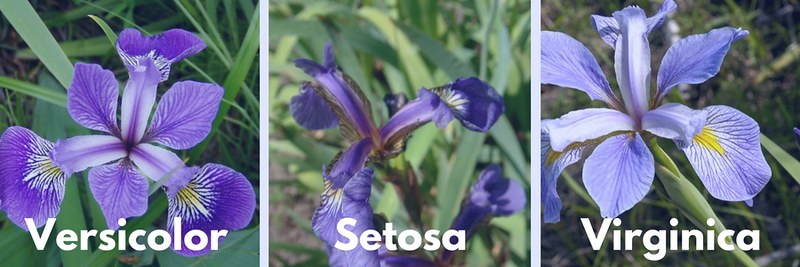
\includegraphics[keepaspectratio]{media/iris_species.jpg}}

}

\caption{The three species of iris in the default data set.}

\end{figure}%

Here is what the data summary looks like.

\begin{Shaded}
\begin{Highlighting}[]
\FunctionTok{summary}\NormalTok{(iris)}
\end{Highlighting}
\end{Shaded}

\begin{verbatim}
  Sepal.Length    Sepal.Width     Petal.Length    Petal.Width   
 Min.   :4.300   Min.   :2.000   Min.   :1.000   Min.   :0.100  
 1st Qu.:5.100   1st Qu.:2.800   1st Qu.:1.600   1st Qu.:0.300  
 Median :5.800   Median :3.000   Median :4.350   Median :1.300  
 Mean   :5.843   Mean   :3.057   Mean   :3.758   Mean   :1.199  
 3rd Qu.:6.400   3rd Qu.:3.300   3rd Qu.:5.100   3rd Qu.:1.800  
 Max.   :7.900   Max.   :4.400   Max.   :6.900   Max.   :2.500  
       Species  
 setosa    :50  
 versicolor:50  
 virginica :50  
                
                
                
\end{verbatim}

\section{Basic Plotting in R}\label{basic-plotting-in-r}

The base \texttt{R} comes with several built-in plotting functions, each
of which is accessed through a single function with a wide array of
optional arguments that modify the overall appearance.

\emph{Histograms - The Density of A Single Data Vector}

\begin{Shaded}
\begin{Highlighting}[]
\FunctionTok{hist}\NormalTok{( iris}\SpecialCharTok{$}\NormalTok{Sepal.Length)}
\end{Highlighting}
\end{Shaded}

\pandocbounded{
\includegraphics[keepaspectratio]{narrative_classic_files/figure-pdf/unnamed-chunk-2-1.pdf}}

You can see that the default values for the \texttt{hist()} function
label the x-axis \& title on the graph have the names of the variable
passed to it, with a y-axis is set to ``Frequency''.

\begin{itemize}
\tightlist
\item
  \texttt{xlab} \& \texttt{ylab}: The names attached to both x- and
  y-axes.
\item
  \texttt{main}: The title on top of the graph.
\item
  \texttt{breaks}: This controls the way in which the original data are
  partitioned (e.g., the width of the bars along the x-axis).

  \begin{itemize}
  \tightlist
  \item
    If you pass a single number, \texttt{n} to this option, the data
    will be partitioned into \texttt{n} bins.
  \item
    If you pass a sequence of values to this, it will use this sequence
    as the boundaries of bins.
  \end{itemize}
\item
  \texttt{col}: The color of the bar (not the border)
\item
  \texttt{probability}: A flag as either \texttt{TRUE} or \texttt{FALSE}
  (the default) to have the y-axis scaled by total likelihood of each
  bins rather than a count of the numbrer of elements in that range.
\end{itemize}

\emph{Density - Estimating the continuous density of data}

\begin{Shaded}
\begin{Highlighting}[]
\NormalTok{d\_sepal.length }\OtherTok{\textless{}{-}} \FunctionTok{density}\NormalTok{( iris}\SpecialCharTok{$}\NormalTok{Sepal.Length )}
\NormalTok{d\_sepal.length}
\end{Highlighting}
\end{Shaded}

\begin{verbatim}

Call:
    density.default(x = iris$Sepal.Length)

Data: iris$Sepal.Length (150 obs.); Bandwidth 'bw' = 0.2736

       x               y           
 Min.   :3.479   Min.   :0.000148  
 1st Qu.:4.790   1st Qu.:0.034088  
 Median :6.100   Median :0.153218  
 Mean   :6.100   Mean   :0.190407  
 3rd Qu.:7.410   3rd Qu.:0.378921  
 Max.   :8.721   Max.   :0.396476  
\end{verbatim}

The \texttt{density()} function estimates a continuous probability
density function for the data and returns an object that has both
\texttt{x} and \texttt{y} values. In fact, it is a special kind of
object.

\begin{Shaded}
\begin{Highlighting}[]
\FunctionTok{class}\NormalTok{(d\_sepal.length)}
\end{Highlighting}
\end{Shaded}

\begin{verbatim}
[1] "density"
\end{verbatim}

Because of this, the general \texttt{plot()} function knows how to plot
these kinds of things.

\begin{Shaded}
\begin{Highlighting}[]
\FunctionTok{plot}\NormalTok{( d\_sepal.length )}
\end{Highlighting}
\end{Shaded}

\pandocbounded{
\includegraphics[keepaspectratio]{narrative_classic_files/figure-pdf/unnamed-chunk-5-1.pdf}}

Now, the general \texttt{plot()} function has \emph{A TON} of options
and is overloaded to be able to plot all kinds of data. In addition to
\texttt{xlab} and \texttt{ylab}, we modify the following:

\begin{itemize}
\tightlist
\item
  \texttt{col}: Color of the line.
\item
  \texttt{lwd}: Line width
\item
  \texttt{bty}: This covers the `box type', which is the square box
  around the plot area. I typically use \texttt{bty="n"} because I hate
  those square boxes around my plots (compare the following 2 plots to
  see the differences). But you do you.
\item
  \texttt{xlim} \& \texttt{ylim}: These dictate the range on both the x-
  and y-axes. It takes a pair of values such as \texttt{c(min,max)} and
  then limits (or extends) that axis to to fill that range.
\end{itemize}

\emph{Scatter Plots - Plotting two variables}

\begin{Shaded}
\begin{Highlighting}[]
\FunctionTok{plot}\NormalTok{( iris}\SpecialCharTok{$}\NormalTok{Sepal.Length, iris}\SpecialCharTok{$}\NormalTok{Sepal.Width  )}
\end{Highlighting}
\end{Shaded}

\pandocbounded{
\includegraphics[keepaspectratio]{narrative_classic_files/figure-pdf/unnamed-chunk-6-1.pdf}}

Here is the most general \texttt{plot()}. The form of the arguments to
this function are x-data and then y-data. The visual representation of
the data is determined by the optional values you pass (or if you do not
pass any optional values, the default is the scatter plot shown above)

{\def\LTcaptype{none} % do not increment counter
\begin{longtable}[]{@{}
  >{\raggedright\arraybackslash}p{(\linewidth - 2\tabcolsep) * \real{0.0855}}
  >{\raggedright\arraybackslash}p{(\linewidth - 2\tabcolsep) * \real{0.9145}}@{}}
\toprule\noalign{}
\begin{minipage}[b]{\linewidth}\raggedright
Parameter
\end{minipage} & \begin{minipage}[b]{\linewidth}\raggedright
Description
\end{minipage} \\
\midrule\noalign{}
\endhead
\bottomrule\noalign{}
\endlastfoot
\texttt{type} & The kind of plot to show ('p'oint, 'l'ine, 'b'oth, or
'o'ver). A point plot is the default. \\
\texttt{pch} & The character (or symbol) being used to plot. There 26
recognized general characters to use for plotting. The default is
\texttt{pch=1}. \\
\texttt{col} & The color of the symbols/lines that are plot. \\
\texttt{cex} & The magnification size of the character being plot. The
default is \texttt{cex=1} and deviation from that will increase
(\(cex > 1\)) or decrease (\(0 < cex < 1\)) the scaling of the
symbols. \\
\texttt{lwd} & The width of any lines in the plot. \\
\texttt{lty} & The type of line to be plot (solid, dashed, etc.) \\
\end{longtable}
}

\pandocbounded{
\includegraphics[keepaspectratio]{narrative_classic_files/figure-pdf/unnamed-chunk-7-1.pdf}}

One of the relevant things you can use the parameter \texttt{pch} for is
to differentiate between groups of observations (such as different
species for example). Instead of giving it one value, pass it a vector
of values whose length is equal to that for x- and y-axis data.

Here is an example where I coerce the \texttt{iris\$Species} data vector
into numeric types and use that for symbols.

\begin{Shaded}
\begin{Highlighting}[]
\NormalTok{symbol }\OtherTok{\textless{}{-}} \FunctionTok{as.numeric}\NormalTok{(iris}\SpecialCharTok{$}\NormalTok{Species)}
\NormalTok{symbol}
\end{Highlighting}
\end{Shaded}

\begin{verbatim}
  [1] 1 1 1 1 1 1 1 1 1 1 1 1 1 1 1 1 1 1 1 1 1 1 1 1 1 1 1 1 1 1 1 1 1 1 1 1 1
 [38] 1 1 1 1 1 1 1 1 1 1 1 1 1 2 2 2 2 2 2 2 2 2 2 2 2 2 2 2 2 2 2 2 2 2 2 2 2
 [75] 2 2 2 2 2 2 2 2 2 2 2 2 2 2 2 2 2 2 2 2 2 2 2 2 2 2 3 3 3 3 3 3 3 3 3 3 3
[112] 3 3 3 3 3 3 3 3 3 3 3 3 3 3 3 3 3 3 3 3 3 3 3 3 3 3 3 3 3 3 3 3 3 3 3 3 3
[149] 3 3
\end{verbatim}

\begin{Shaded}
\begin{Highlighting}[]
\FunctionTok{plot}\NormalTok{( iris}\SpecialCharTok{$}\NormalTok{Sepal.Length, iris}\SpecialCharTok{$}\NormalTok{Sepal.Width, }\AttributeTok{pch=}\NormalTok{symbol )}
\end{Highlighting}
\end{Shaded}

\pandocbounded{
\includegraphics[keepaspectratio]{narrative_classic_files/figure-pdf/unnamed-chunk-9-1.pdf}}

We can use the same technique to use \texttt{col} instead of
\texttt{pch}. Here I make a vector of color names and then use the
previously defined in the variable \texttt{symbol}.

\begin{Shaded}
\begin{Highlighting}[]
\NormalTok{raw\_colors }\OtherTok{\textless{}{-}} \FunctionTok{c}\NormalTok{(}\StringTok{"red"}\NormalTok{,}\StringTok{"gold"}\NormalTok{,}\StringTok{"forestgreen"}\NormalTok{)}
\NormalTok{colors }\OtherTok{\textless{}{-}}\NormalTok{ raw\_colors[ symbol ]}
\NormalTok{colors[}\DecValTok{1}\SpecialCharTok{:}\DecValTok{10}\NormalTok{]}
\end{Highlighting}
\end{Shaded}

\begin{verbatim}
 [1] "red" "red" "red" "red" "red" "red" "red" "red" "red" "red"
\end{verbatim}

In addition to the general form for the function \texttt{plot(x,y)} we
used above, we can use an alternative designation based upon what is
called the \emph{functional form}. The \emph{functional form} is how we
designate functions in \texttt{R}, such as regression anlaysis. This
basic syntax for this is \texttt{y\ \textasciitilde{}\ x}, that is the
response variable (on the y-axis) is a function of the predictor (on the
x-axis).

For simplicty, I'll make \texttt{x} and \texttt{y} varibles pointing to
the same same data as in the previous graph.

\begin{Shaded}
\begin{Highlighting}[]
\NormalTok{y }\OtherTok{\textless{}{-}}\NormalTok{ iris}\SpecialCharTok{$}\NormalTok{Sepal.Width}
\NormalTok{x }\OtherTok{\textless{}{-}}\NormalTok{ iris}\SpecialCharTok{$}\NormalTok{Sepal.Length}
\end{Highlighting}
\end{Shaded}

Then, the \texttt{plot()} function can be written as (including all the
fancy additional stuff we just described):

\begin{Shaded}
\begin{Highlighting}[]
\FunctionTok{plot}\NormalTok{( y }\SpecialCharTok{\textasciitilde{}}\NormalTok{ x , }
      \AttributeTok{col=}\NormalTok{colors, }
      \AttributeTok{pch=}\DecValTok{20}\NormalTok{, }
      \AttributeTok{bty=}\StringTok{"n"}\NormalTok{, }
      \AttributeTok{xlab=}\StringTok{"Sepal Length"}\NormalTok{, }\AttributeTok{ylab=}\StringTok{"Sepal Width"}\NormalTok{)}
\end{Highlighting}
\end{Shaded}

\pandocbounded{
\includegraphics[keepaspectratio]{narrative_classic_files/figure-pdf/unnamed-chunk-12-1.pdf}}

This is \textbf{much} easier to read (also notice how I used serveral
lines to put in all the options to the plot function for legibility).

\emph{Bar Plots - Quantifying Counts}

The \texttt{barplot} function takes a set of heights, one for each bar.
Let's quickly grab the mean length for sepals across all three species.
There are many ways to do this, here are two, the first being more
pedantic and the second more concise.

The \texttt{iris} data is in a \texttt{data.frame} that has a column
designating the species. We can see which ones using \texttt{unique()}.

\begin{Shaded}
\begin{Highlighting}[]
\FunctionTok{unique}\NormalTok{( iris}\SpecialCharTok{$}\NormalTok{Species )}
\end{Highlighting}
\end{Shaded}

\begin{verbatim}
[1] setosa     versicolor virginica 
Levels: setosa versicolor virginica
\end{verbatim}

To estimate the mean for each species, we can take values in
\texttt{iris\$Sepal.Length} for each level of \texttt{iris\$Species}
using indices.

\begin{Shaded}
\begin{Highlighting}[]
\NormalTok{mu.Setosa }\OtherTok{\textless{}{-}} \FunctionTok{mean}\NormalTok{( iris}\SpecialCharTok{$}\NormalTok{Sepal.Length[ iris}\SpecialCharTok{$}\NormalTok{Species }\SpecialCharTok{==} \StringTok{"setosa"}\NormalTok{ ])}
\NormalTok{mu.Versicolor }\OtherTok{\textless{}{-}} \FunctionTok{mean}\NormalTok{( iris}\SpecialCharTok{$}\NormalTok{Sepal.Length[ iris}\SpecialCharTok{$}\NormalTok{Species }\SpecialCharTok{==} \StringTok{"versicolor"}\NormalTok{ ])}
\NormalTok{mu.Virginica }\OtherTok{\textless{}{-}} \FunctionTok{mean}\NormalTok{( iris}\SpecialCharTok{$}\NormalTok{Sepal.Length[ iris}\SpecialCharTok{$}\NormalTok{Species }\SpecialCharTok{==} \StringTok{"virginica"}\NormalTok{ ])}

\NormalTok{meanSepalLength }\OtherTok{\textless{}{-}} \FunctionTok{c}\NormalTok{( mu.Setosa, mu.Versicolor, mu.Virginica )}
\NormalTok{meanSepalLength}
\end{Highlighting}
\end{Shaded}

\begin{verbatim}
[1] 5.006 5.936 6.588
\end{verbatim}

When we plot these data using \texttt{barplot()} we pass the values and
set the names of the bars us

\begin{Shaded}
\begin{Highlighting}[]
\FunctionTok{barplot}\NormalTok{( meanSepalLength, }
         \AttributeTok{names.arg =} \FunctionTok{c}\NormalTok{(}\StringTok{"setosa"}\NormalTok{,}\StringTok{"versicolor"}\NormalTok{,}\StringTok{"virginica"}\NormalTok{), }
         \AttributeTok{xlab=}\StringTok{"Iris Species"}\NormalTok{,}
         \AttributeTok{ylab=}\StringTok{"Mean Sepal Length"}\NormalTok{)}
\end{Highlighting}
\end{Shaded}

\pandocbounded{
\includegraphics[keepaspectratio]{narrative_classic_files/figure-pdf/unnamed-chunk-15-1.pdf}}

The second way to do this is to use the \texttt{by()} function (see
\texttt{?by} for the complete help file). The \texttt{by} function takes
the following objects:

\begin{itemize}
\tightlist
\item
  The raw data to use as measurements. Here we will use
  \texttt{iris\$Sepal.Length} as the raw data.
\item
  Data designating groups to partition the raw data into (we will use
  \texttt{iris\$Species}).
\item
  The function that you want to use on each group. (here we will ask for
  the mean).
\end{itemize}

\begin{Shaded}
\begin{Highlighting}[]
\NormalTok{meanSepalLength }\OtherTok{\textless{}{-}} \FunctionTok{by}\NormalTok{( iris}\SpecialCharTok{$}\NormalTok{Sepal.Length, iris}\SpecialCharTok{$}\NormalTok{Species, mean )}
\NormalTok{meanSepalLength}
\end{Highlighting}
\end{Shaded}

\begin{verbatim}
iris$Species: setosa
[1] 5.006
------------------------------------------------------------ 
iris$Species: versicolor
[1] 5.936
------------------------------------------------------------ 
iris$Species: virginica
[1] 6.588
\end{verbatim}

The data returned from this function is both \texttt{numeric} \emph{and}
has a name set for each value.

\begin{Shaded}
\begin{Highlighting}[]
\FunctionTok{is.numeric}\NormalTok{( meanSepalLength )}
\end{Highlighting}
\end{Shaded}

\begin{verbatim}
[1] TRUE
\end{verbatim}

\begin{Shaded}
\begin{Highlighting}[]
\FunctionTok{names}\NormalTok{( meanSepalLength )}
\end{Highlighting}
\end{Shaded}

\begin{verbatim}
[1] "setosa"     "versicolor" "virginica" 
\end{verbatim}

Then when we pass that to \texttt{barplot()} the column labels are set
automatically (e.g., no need to set \texttt{names.arg} as above).

\begin{Shaded}
\begin{Highlighting}[]
\FunctionTok{barplot}\NormalTok{( meanSepalLength, }
         \AttributeTok{xlab =} \StringTok{"Iris Species"}\NormalTok{,}
         \AttributeTok{ylab =} \StringTok{"Average Sepal Length"}\NormalTok{)}
\end{Highlighting}
\end{Shaded}

\pandocbounded{
\includegraphics[keepaspectratio]{narrative_classic_files/figure-pdf/unnamed-chunk-18-1.pdf}}

\emph{Boxplots - High density information}

A boxplot contains a high amount of information content and is
appropriate when the groupings on the x-axis are categorical. For each
category, the graphical representation includes:

\begin{itemize}
\tightlist
\item
  The median value for the raw data
\item
  A box indicating the area between the first and third quartile (e.g,.
  the values enclosing the 25\% - 75\% of the data). The top and bottoms
  are often referred to as the \emph{hinges} of the box.
\item
  A notch (if requested), represents confidence around the estimate of
  the median.
\item
  Whiskers extending out to shows \(\pm 1.5 * IQR\) (the Inner Quartile
  Range)
\item
  Any points of the data that extend beyond the whiskers are plot as
  points.
\end{itemize}

For legibility, we can use the \emph{functional} form for the plots as
well as separate out the \texttt{data.frame} from the columns using the
optional \texttt{data=} argument.

\begin{Shaded}
\begin{Highlighting}[]
\FunctionTok{boxplot}\NormalTok{( Sepal.Length }\SpecialCharTok{\textasciitilde{}}\NormalTok{ Species, }
         \AttributeTok{data =}\NormalTok{ iris, }
         \AttributeTok{notch=}\ConstantTok{TRUE}\NormalTok{, }
         \AttributeTok{ylab=}\StringTok{"Sepal Length"}\NormalTok{ )}
\end{Highlighting}
\end{Shaded}

\pandocbounded{
\includegraphics[keepaspectratio]{narrative_classic_files/figure-pdf/unnamed-chunk-19-1.pdf}}

\section{Colors}\label{colors}

\emph{Named Colors - } There are 657 pre-defined, named colors built
into the base \texttt{R} distribution. Here is a random selection of
those values.

\begin{Shaded}
\begin{Highlighting}[]
\NormalTok{randomColors }\OtherTok{\textless{}{-}} \FunctionTok{sample}\NormalTok{( }\FunctionTok{colors}\NormalTok{(), }\AttributeTok{size =} \FunctionTok{nrow}\NormalTok{(iris) )}
\FunctionTok{head}\NormalTok{(randomColors)}
\end{Highlighting}
\end{Shaded}

\begin{verbatim}
[1] "grey57"     "rosybrown1" "cadetblue1" "grey3"      "gray61"    
[6] "maroon"    
\end{verbatim}

To use these colors, you can specify them by name for either all the
elements

\begin{Shaded}
\begin{Highlighting}[]
\FunctionTok{boxplot}\NormalTok{( Sepal.Length }\SpecialCharTok{\textasciitilde{}}\NormalTok{ Species, }
         \AttributeTok{data =}\NormalTok{ iris, }
         \AttributeTok{col =}\NormalTok{ randomColors[}\DecValTok{1}\NormalTok{],}
         \AttributeTok{notch=}\ConstantTok{TRUE}\NormalTok{, }
         \AttributeTok{ylab=}\StringTok{"Sepal Length"}\NormalTok{ )}
\end{Highlighting}
\end{Shaded}

\pandocbounded{
\includegraphics[keepaspectratio]{narrative_classic_files/figure-pdf/unnamed-chunk-21-1.pdf}}

\emph{or} for each element individually.

\begin{Shaded}
\begin{Highlighting}[]
\FunctionTok{boxplot}\NormalTok{( Sepal.Length }\SpecialCharTok{\textasciitilde{}}\NormalTok{ Species, }
         \AttributeTok{data =}\NormalTok{ iris, }
         \AttributeTok{col =}\NormalTok{ randomColors[}\DecValTok{1}\SpecialCharTok{:}\DecValTok{3}\NormalTok{],}
         \AttributeTok{notch=}\ConstantTok{TRUE}\NormalTok{, }
         \AttributeTok{ylab=}\StringTok{"Sepal Length"}\NormalTok{ )}
\end{Highlighting}
\end{Shaded}

\pandocbounded{
\includegraphics[keepaspectratio]{narrative_classic_files/figure-pdf/unnamed-chunk-22-1.pdf}}

\emph{Hex Colors: } You can also use hexadecimal representations of
colors, which is most commonly used on the internet. A hex
representation of colors consists of red, green, and blue values encoded
as numbers in base 16 (e.g., the single digits 0, 1, 2, 3, 4, 5, 6, 7,
8, 9, A, B, C, D, E, F). There are a lot of great resources on the
internet for color themes that report red, green, blue and hex values. I
often use the \href{https://coolors.co}{coolors.co} website to look for
themes that go well together for slides or presentations.

\emph{Color Brewer} Finally, there is an interesting website at
\href{https://colorbrewer2.org}{colorbrewer2.org} that has some
interesting built-in palettes. There is an associated library that makes
creating palettes for plots really easy and as you get more expreienced
with \texttt{R}, you will find this very helpful. For quick
visualizations and estimation of built-in color palettes, you can look
at the \href{https://colorbrewer2.org}{website} (below).

\pandocbounded{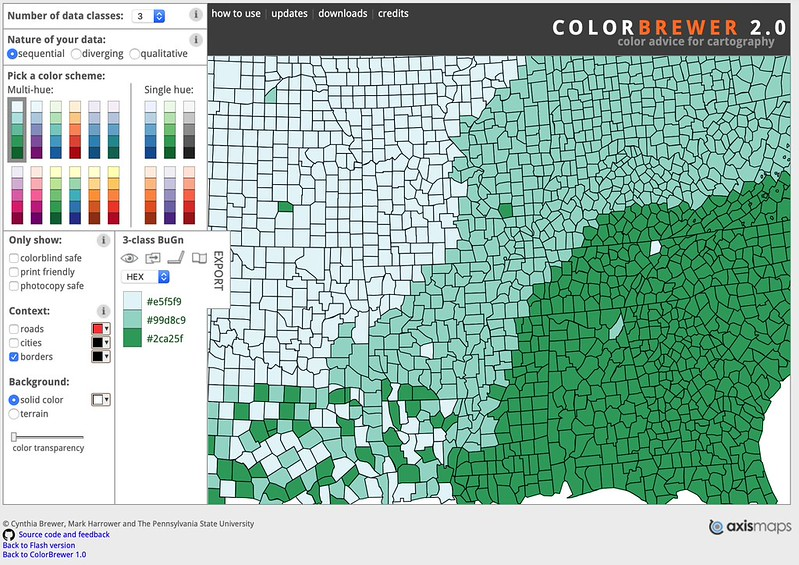
\includegraphics[keepaspectratio,alt={ColorBrewer Site}]{media/colorbrewer_site.jpg}}
or look at the colors in \texttt{R}

\begin{Shaded}
\begin{Highlighting}[]
\FunctionTok{library}\NormalTok{(RColorBrewer)}
\FunctionTok{display.brewer.all}\NormalTok{()}
\end{Highlighting}
\end{Shaded}

\pandocbounded{
\includegraphics[keepaspectratio]{narrative_classic_files/figure-pdf/unnamed-chunk-23-1.pdf}}

There are three basic kinds of palettes: divergent, qualitative, and
sequential. Each of these built-in palletes has a maximum number of
colors available (though as you see below we can use them to interpolate
larger sets) as well as indications if the palette is safe for
colorblind individuals.

\begin{Shaded}
\begin{Highlighting}[]
\NormalTok{brewer.pal.info}
\end{Highlighting}
\end{Shaded}

\begin{verbatim}
         maxcolors category colorblind
BrBG            11      div       TRUE
PiYG            11      div       TRUE
PRGn            11      div       TRUE
PuOr            11      div       TRUE
RdBu            11      div       TRUE
RdGy            11      div      FALSE
RdYlBu          11      div       TRUE
RdYlGn          11      div      FALSE
Spectral        11      div      FALSE
Accent           8     qual      FALSE
Dark2            8     qual       TRUE
Paired          12     qual       TRUE
Pastel1          9     qual      FALSE
Pastel2          8     qual      FALSE
Set1             9     qual      FALSE
Set2             8     qual       TRUE
Set3            12     qual      FALSE
Blues            9      seq       TRUE
BuGn             9      seq       TRUE
BuPu             9      seq       TRUE
GnBu             9      seq       TRUE
Greens           9      seq       TRUE
Greys            9      seq       TRUE
Oranges          9      seq       TRUE
OrRd             9      seq       TRUE
PuBu             9      seq       TRUE
PuBuGn           9      seq       TRUE
PuRd             9      seq       TRUE
Purples          9      seq       TRUE
RdPu             9      seq       TRUE
Reds             9      seq       TRUE
YlGn             9      seq       TRUE
YlGnBu           9      seq       TRUE
YlOrBr           9      seq       TRUE
YlOrRd           9      seq       TRUE
\end{verbatim}

It is very helpful to look at the different kinds of data palettes
available and I'll show you how to use them below when we color in the
states based upon population size at the end of this document.

\section{Annotations}\label{annotations}

You can easily add text onto a graph using the \texttt{text()} function.
Here is the correlation between the sepal length and width (the function
\texttt{cor.test()} does the statistical test).

\begin{Shaded}
\begin{Highlighting}[]
\NormalTok{cor }\OtherTok{\textless{}{-}} \FunctionTok{cor.test}\NormalTok{( iris}\SpecialCharTok{$}\NormalTok{Sepal.Length, iris}\SpecialCharTok{$}\NormalTok{Sepal.Width )}
\NormalTok{cor}
\end{Highlighting}
\end{Shaded}

\begin{verbatim}

    Pearson's product-moment correlation

data:  iris$Sepal.Length and iris$Sepal.Width
t = -1.4403, df = 148, p-value = 0.1519
alternative hypothesis: true correlation is not equal to 0
95 percent confidence interval:
 -0.27269325  0.04351158
sample estimates:
       cor 
-0.1175698 
\end{verbatim}

We can put the correlation and the p-value on the plot

\begin{Shaded}
\begin{Highlighting}[]
\NormalTok{cor.text }\OtherTok{\textless{}{-}} \FunctionTok{paste}\NormalTok{( }\StringTok{"r = "}\NormalTok{, }\FunctionTok{format}\NormalTok{( cor}\SpecialCharTok{$}\NormalTok{estimate, }\AttributeTok{digits=}\DecValTok{4}\NormalTok{), }\StringTok{"; P = "}\NormalTok{, }\FunctionTok{format}\NormalTok{( cor}\SpecialCharTok{$}\NormalTok{p.value, }\AttributeTok{digits=}\DecValTok{4}\NormalTok{ ), }\AttributeTok{sep=}\StringTok{""}\NormalTok{ ) }
\NormalTok{cor.text}
\end{Highlighting}
\end{Shaded}

\begin{verbatim}
[1] "r = -0.1176; P = 0.1519"
\end{verbatim}

The we can the overlay this onto an existing plot. For the
\texttt{text()} function, we need to give the x- and y- coordinates
where you want it put onto the coordinate space of the existing graph.

\begin{Shaded}
\begin{Highlighting}[]
\FunctionTok{plot}\NormalTok{( y }\SpecialCharTok{\textasciitilde{}}\NormalTok{ x , }
      \AttributeTok{col=}\NormalTok{colors, }
      \AttributeTok{pch=}\DecValTok{20}\NormalTok{, }
      \AttributeTok{bty=}\StringTok{"n"}\NormalTok{, }
      \AttributeTok{xlab=}\StringTok{"Sepal Length"}\NormalTok{, }\AttributeTok{ylab=}\StringTok{"Sepal Width"}\NormalTok{)}
\FunctionTok{text}\NormalTok{( }\FloatTok{7.4}\NormalTok{, }\FloatTok{4.2}\NormalTok{, cor.text )}
\end{Highlighting}
\end{Shaded}

\pandocbounded{
\includegraphics[keepaspectratio]{narrative_classic_files/figure-pdf/unnamed-chunk-27-1.pdf}}

\chapter{\texorpdfstring{\texttt{ggplot2}
Graphics}{ggplot2 Graphics}}\label{ggplot2-graphics}

\pandocbounded{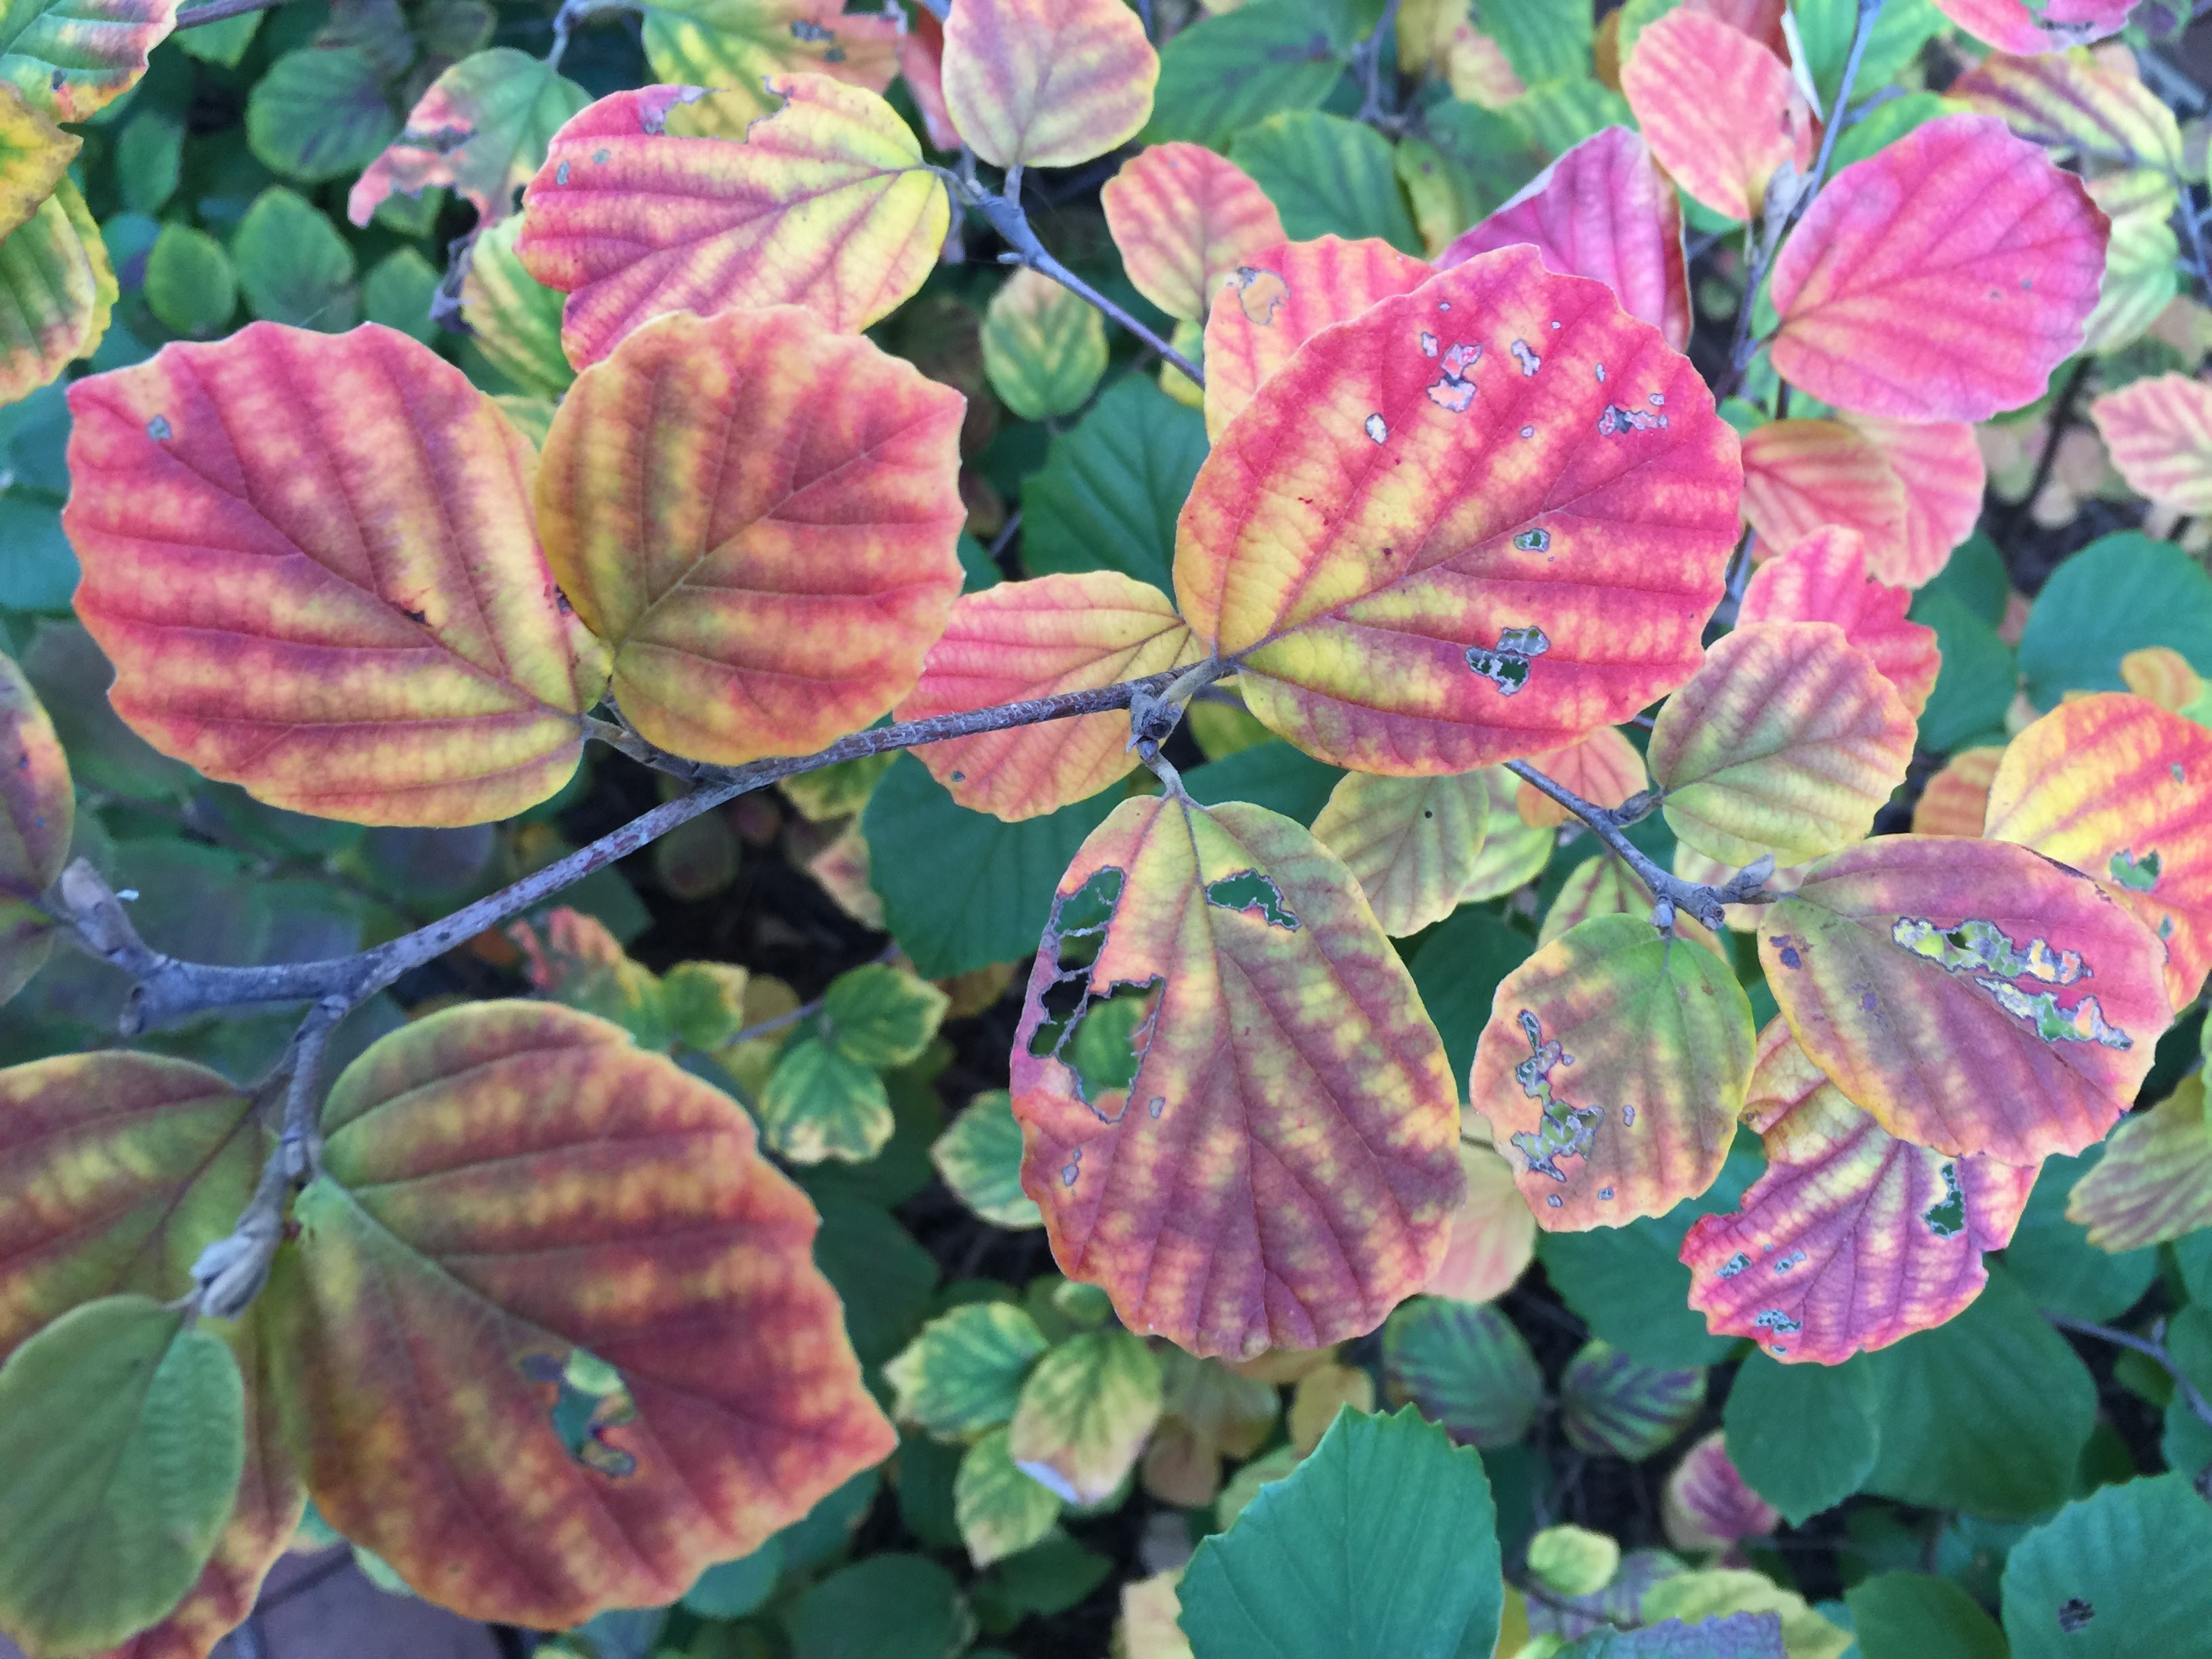
\includegraphics[keepaspectratio]{media/chapter_ggplot.jpg}}

\begin{quote}
The \texttt{ggplot2} library is a gramattical approach to data display.
\end{quote}

\section{Lecture Materials}\label{lecture-materials-7}

\begin{quote}
\textbf{Lecture Slides:} Available interactively in the
\href{https://dyerlabteaching.github.io/Graphics-That-Do-Not-Suck/slides.html\#/title-slide}{online
version}
\end{quote}

\begin{figure}[H]

{\centering \pandocbounded{
\includegraphics[keepaspectratio]{media/slides_ggplot.png}}

}

\caption{Lecture Slides}

\end{figure}%

In base \texttt{R}, the graphics are generally produced by adding a lot
of optional arguments to a single function such as \texttt{plot()} or
\texttt{barplot()} or \texttt{boxplot()}. We can get some kinds of
overlays using \texttt{text()} or \texttt{points()} or \texttt{lines()}
but there is not a cohesive framework for setting this up. For even
moderately complex graphical display, these approaches become unwieldy
when we have to cram all that information into extra optional arguments.

\begin{figure}[H]

{\centering \pandocbounded{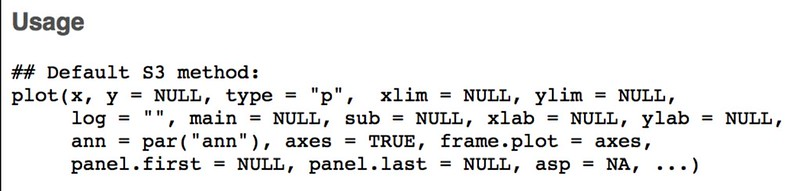
\includegraphics[keepaspectratio]{media/base_plot_r.jpg}}

}

\caption{base plot in R}

\end{figure}%

Consider the graph below whose data are from a 2011 article in \emph{The
Economist} measuring human development and perception of corruption for
173 countries (Figure~\ref{fig-economist}). Both the amount of data and
the way in which the data are displayed (physically and aesthetically)
are somewhat complex.

\begin{figure}[H]

\centering{

\pandocbounded{
\includegraphics[keepaspectratio]{narrative_ggplot_files/figure-pdf/fig-economist-1.pdf}}

}

\caption{\label{fig-economist}Corruption and Human Develoment among OECD
countries from The Economist magazine.}

\end{figure}%

This graphic is constructed from several \emph{additive}
components\footnote{Pielou EC, (1984) The interpretation of ecological
  data: A primer on classification and ordination. 288pg. ISBN:
  \href{https://www.wiley.com/en-us/The+Interpretation+of+Ecological+Data\%3A+A+Primer+on+Classification+and+Ordination-p-9780471889502}{978-0-471-88950-2}}
including:

\begin{itemize}
\tightlist
\item
  A raw \texttt{data.frame} that has several kinds of data (CPI, HDI,
  region, names, etc.).\\
\item
  A \emph{aesthetic} statement indicating which columns of data to use
  and how to use them in the plot (designating x-axis vs color, etc.).\\
\item
  An estimate of a trendline through the data (the red one), which
  displays a statistical summary of the raw data.\\
\item
  A set of geometric overlays for the points which include size and
  shape configurations.\\
\item
  Specified color scheme for the regions.
\item
  Labeling of a subset of the data (which is done using a separate
  \texttt{data.frame} derived from the first).
\item
  Labels on axes.
\item
  A legend positioned in a specific fashion.\\
\item
  A title over the whole thing.\\
\item
  A theme for the rest of the coloring and customized lines and grids.
\end{itemize}

Truth be told (and you can look at the RMD of this file to verify), this
one graphic required 42 relatively terse lines of code to construct! If
all of that code was stuffed into the \emph{optional arguments} for a
few functions, I think I would go mad.

Luckily for us, there are people who spend a lot of time working on
these issues and thinking about how to best help us effectively display
data. One of these individuals was Leland Wilkinson, whose book
\emph{The Grammar of Graphics} defined just such a system.

\begin{figure}[H]

{\centering \pandocbounded{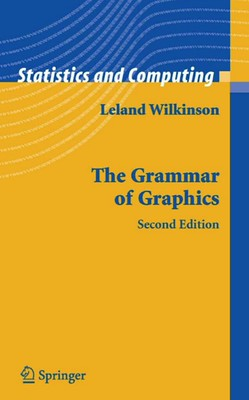
\includegraphics[keepaspectratio]{media/grammar_of_graphics.jpg}}

}

\caption{The Grammar of Graphics by Leland Wilkinson}

\end{figure}%

This philosophy has been inserted into the \texttt{R} Ecosystem by
Hadley Wickham in the \texttt{ggplot2} library, which is descbribed as:

\begin{quote}
A system for `declaratively' creating graphics, based on ``The Grammar
of Graphics''. You provide the data, tell `ggplot2' how to map variables
to aesthetics, what graphical primitives to use, and it takes care of
the details.
\end{quote}

Throughout the majority of this course, we will be using this library
and this approach for all but the most trivial of graphical displays.

\section{Basic ggplot}\label{basic-ggplot}

As outlined above, the basis of this appraoch is an additive (and
iterative) process of creating a graphic. This all starts with the data.
For our purposes, we will use the same iris \texttt{data.frame} as in
the previous section on base graphics.

\begin{figure}[H]

{\centering \pandocbounded{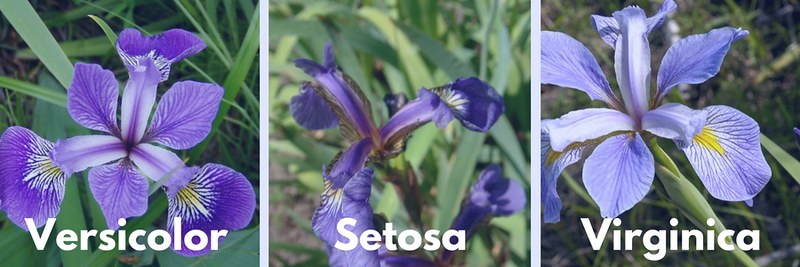
\includegraphics[keepaspectratio]{media/iris_species.jpg}}

}

\caption{The iris data}

\end{figure}%

\begin{Shaded}
\begin{Highlighting}[]
\FunctionTok{summary}\NormalTok{( iris )}
\end{Highlighting}
\end{Shaded}

\begin{verbatim}
  Sepal.Length    Sepal.Width     Petal.Length    Petal.Width   
 Min.   :4.300   Min.   :2.000   Min.   :1.000   Min.   :0.100  
 1st Qu.:5.100   1st Qu.:2.800   1st Qu.:1.600   1st Qu.:0.300  
 Median :5.800   Median :3.000   Median :4.350   Median :1.300  
 Mean   :5.843   Mean   :3.057   Mean   :3.758   Mean   :1.199  
 3rd Qu.:6.400   3rd Qu.:3.300   3rd Qu.:5.100   3rd Qu.:1.800  
 Max.   :7.900   Max.   :4.400   Max.   :6.900   Max.   :2.500  
       Species  
 setosa    :50  
 versicolor:50  
 virginica :50  
                
                
                
\end{verbatim}

We start building a graphic using the \texttt{ggplot()} function and
passing it the \texttt{data.frame} object. This will initialize the
graphic, though it will not plot anything.

\begin{Shaded}
\begin{Highlighting}[]
\FunctionTok{library}\NormalTok{(ggplot2)}

\FunctionTok{ggplot}\NormalTok{( iris )}
\end{Highlighting}
\end{Shaded}

\pandocbounded{
\includegraphics[keepaspectratio]{narrative_ggplot_files/figure-pdf/unnamed-chunk-2-1.pdf}}

Next, we need to tell the plot which variables it will be using from the
\texttt{data.frame}. For simplicity, we do not need to make special data
objects with just the variables we want to plot, we can pass around the
whole \texttt{data.frame} object and just indicate to ggplot which ones
we want to use by specifying the \emph{aesthetics} to be used.

\begin{Shaded}
\begin{Highlighting}[]
\FunctionTok{ggplot}\NormalTok{( iris , }\FunctionTok{aes}\NormalTok{( }\AttributeTok{x=}\NormalTok{Sepal.Length ) )}
\end{Highlighting}
\end{Shaded}

\pandocbounded{
\includegraphics[keepaspectratio]{narrative_ggplot_files/figure-pdf/unnamed-chunk-3-1.pdf}}

At this point, there is enough information to make an axis in the graph
because the underlying data has been identified. What has not been
specified to date is the way in which we want to represent the data. To
do this, we add geometries to the graph. In this case, I'm going to add
a histogram

\begin{Shaded}
\begin{Highlighting}[]
\FunctionTok{ggplot}\NormalTok{( iris, }\FunctionTok{aes}\NormalTok{(}\AttributeTok{x=}\NormalTok{Sepal.Length) ) }\SpecialCharTok{+} \FunctionTok{geom\_histogram}\NormalTok{()}
\end{Highlighting}
\end{Shaded}

\begin{verbatim}
`stat_bin()` using `bins = 30`. Pick better value `binwidth`.
\end{verbatim}

\pandocbounded{
\includegraphics[keepaspectratio]{narrative_ggplot_files/figure-pdf/unnamed-chunk-4-1.pdf}}

Now we have a base graph!

\section{Aestheics and Scope}\label{aestheics-and-scope}

The location of the data and the \texttt{aes()} determines the
\emph{scope} of the assignment. What I mean by this is:

\begin{itemize}
\tightlist
\item
  If the data and \texttt{aes()} is in the the \texttt{ggplot()}
  function, then everything in the whole plot \emph{inherits} that
  assignment.
\item
  If you put them in one or more of the components you add to
  \texttt{ggplot()} then the they are localized to \emph{only} those
  layers.
\end{itemize}

So the following statements are all identical for this most basic of
plots.

\begin{Shaded}
\begin{Highlighting}[]
\FunctionTok{ggplot}\NormalTok{( iris, }\FunctionTok{aes}\NormalTok{(}\AttributeTok{x=}\NormalTok{Sepal.Length) ) }\SpecialCharTok{+} \FunctionTok{geom\_histogram}\NormalTok{()}
\FunctionTok{ggplot}\NormalTok{( iris ) }\SpecialCharTok{+} \FunctionTok{geom\_historgram}\NormalTok{( }\FunctionTok{aes}\NormalTok{(}\AttributeTok{x=}\NormalTok{Sepal.Length) )}
\FunctionTok{ggplot}\NormalTok{() }\SpecialCharTok{+} \FunctionTok{geom\_histogram}\NormalTok{( }\FunctionTok{aes}\NormalTok{(}\AttributeTok{x=}\NormalTok{Sepal.Length), }\AttributeTok{data=}\NormalTok{iris)}
\end{Highlighting}
\end{Shaded}

\begin{itemize}
\tightlist
\item
  In the first case, the \texttt{geom\_histogram()} inherits both data
  and aesthetics from \texttt{ggplot()}.\\
\item
  In the second one, it inherits only the data but has it's own
  specification for aesthetics.
\item
  In the last one, \texttt{ggplot()} only specifies the presence of a
  graph and all the data and aesthetics are localized within
  \texttt{geom\_histogram()} function.
\end{itemize}

Where this becomes important is when we want to make more complicated
graphics like the one above. The data that has the country CDI and HDI
also has the names of the countries. However, only a subset of the
country names are plot. This is because both the geometric layer and the
text layer that has the names are using different \texttt{data.frame}
objects.

Here is a more simplistic example where I overlay a density plot (as a
red line) on top of the histogram.

\begin{Shaded}
\begin{Highlighting}[]
\FunctionTok{ggplot}\NormalTok{( iris, }\FunctionTok{aes}\NormalTok{(}\AttributeTok{x=}\NormalTok{Sepal.Length) ) }\SpecialCharTok{+} \FunctionTok{geom\_histogram}\NormalTok{() }\SpecialCharTok{+} \FunctionTok{geom\_density}\NormalTok{( }\AttributeTok{col=}\StringTok{"red"}\NormalTok{)}
\end{Highlighting}
\end{Shaded}

\begin{verbatim}
`stat_bin()` using `bins = 30`. Pick better value `binwidth`.
\end{verbatim}

\pandocbounded{
\includegraphics[keepaspectratio]{narrative_ggplot_files/figure-pdf/unnamed-chunk-6-1.pdf}}

Both the \texttt{geom\_histogram} and the \texttt{geom\_density} use the
same data and same specification for how to deal with the y-axis.
However, the density is depicted as a frequency on the y-axis whereas
the histogram uses counts. Also notice how the \texttt{col="red"} is
localized just for the \texttt{geom\_density()} layer.

We can override the way in which \texttt{geom\_histogram} uses the
y-axis by changing the \emph{aesthetics} for that particular geometric
layer. Here, I'm goint to add another \texttt{aes()} just within the
\texttt{geom\_histogram()} function and have it treat y as the density
rather than the count (yes that is two periods before and after the word
density).

\begin{Shaded}
\begin{Highlighting}[]
\FunctionTok{ggplot}\NormalTok{( iris, }\FunctionTok{aes}\NormalTok{(}\AttributeTok{x=}\NormalTok{Sepal.Length) ) }\SpecialCharTok{+} \FunctionTok{geom\_histogram}\NormalTok{(}\FunctionTok{aes}\NormalTok{(}\AttributeTok{y=}\NormalTok{..density..)) }\SpecialCharTok{+} \FunctionTok{geom\_density}\NormalTok{( }\AttributeTok{col=}\StringTok{"red"}\NormalTok{ )}
\end{Highlighting}
\end{Shaded}

\begin{verbatim}
Warning: The dot-dot notation (`..density..`) was deprecated in ggplot2 3.4.0.
i Please use `after_stat(density)` instead.
\end{verbatim}

\begin{verbatim}
`stat_bin()` using `bins = 30`. Pick better value `binwidth`.
\end{verbatim}

\pandocbounded{
\includegraphics[keepaspectratio]{narrative_ggplot_files/figure-pdf/unnamed-chunk-7-1.pdf}}

By default, everything inside the \texttt{ggplot()} function call is
inherited by all the remaining components unless it is specifically
overridden. Here is a more pedantic version where only the raw
\texttt{data.frame} is in the \texttt{ggplot} and the rest is in each of
the geometric layers.

\begin{Shaded}
\begin{Highlighting}[]
\FunctionTok{ggplot}\NormalTok{( iris ) }\SpecialCharTok{+} 
  \FunctionTok{geom\_histogram}\NormalTok{( }\FunctionTok{aes}\NormalTok{(}\AttributeTok{x=}\NormalTok{Sepal.Length, }\AttributeTok{y=}\NormalTok{..density..) ) }\SpecialCharTok{+} 
  \FunctionTok{geom\_density}\NormalTok{( }\FunctionTok{aes}\NormalTok{(}\AttributeTok{x=}\NormalTok{Sepal.Length), }\AttributeTok{col=}\StringTok{"red"}\NormalTok{, }\AttributeTok{lwd=}\DecValTok{2}\NormalTok{)}
\end{Highlighting}
\end{Shaded}

\begin{verbatim}
`stat_bin()` using `bins = 30`. Pick better value `binwidth`.
\end{verbatim}

\pandocbounded{
\includegraphics[keepaspectratio]{narrative_ggplot_files/figure-pdf/unnamed-chunk-8-1.pdf}}

\section{Labels \& Titles}\label{labels-titles}

Just like we added geometric layers to the plot to make histograms and
densities, we do the same for labels and titles.

\begin{Shaded}
\begin{Highlighting}[]
\FunctionTok{ggplot}\NormalTok{( iris,  }\FunctionTok{aes}\NormalTok{(}\AttributeTok{x=}\NormalTok{Sepal.Length) ) }\SpecialCharTok{+} 
  \FunctionTok{geom\_histogram}\NormalTok{( }\FunctionTok{aes}\NormalTok{(}\AttributeTok{y=}\NormalTok{..density..), }\AttributeTok{bins =} \DecValTok{10}\NormalTok{, }\AttributeTok{fill=}\StringTok{"lightgray"}\NormalTok{, }\AttributeTok{col=}\StringTok{"darkgrey"}\NormalTok{ ) }\SpecialCharTok{+} 
  \FunctionTok{geom\_density}\NormalTok{( }\AttributeTok{col=}\StringTok{"red"}\NormalTok{, }\AttributeTok{lwd=}\FloatTok{1.5}\NormalTok{) }\SpecialCharTok{+} 
  \FunctionTok{xlab}\NormalTok{(}\StringTok{"Length"}\NormalTok{) }\SpecialCharTok{+} \FunctionTok{ylab}\NormalTok{(}\StringTok{"Density"}\NormalTok{) }\SpecialCharTok{+} 
  \FunctionTok{ggtitle}\NormalTok{(}\StringTok{"Sepal Lengths for Three Iris Species"}\NormalTok{)}
\end{Highlighting}
\end{Shaded}

\pandocbounded{
\includegraphics[keepaspectratio]{narrative_ggplot_files/figure-pdf/unnamed-chunk-9-1.pdf}}

\section{Scatter Plots}\label{scatter-plots}

With two columns of data, we can make the old scatter plot using the
\texttt{geom\_point()} function.

\begin{Shaded}
\begin{Highlighting}[]
\FunctionTok{ggplot}\NormalTok{( iris, }\FunctionTok{aes}\NormalTok{(}\AttributeTok{x=}\NormalTok{Sepal.Length, }\AttributeTok{y=}\NormalTok{Sepal.Width) ) }\SpecialCharTok{+} \FunctionTok{geom\_point}\NormalTok{( }\AttributeTok{col=}\StringTok{"purple"}\NormalTok{) }
\end{Highlighting}
\end{Shaded}

\pandocbounded{
\includegraphics[keepaspectratio]{narrative_ggplot_files/figure-pdf/unnamed-chunk-10-1.pdf}}

In this plot, we are hiding some of the information by having all the
points be the same color and shape. We could have a \texttt{geom\_point}
for each species as follows:

\begin{Shaded}
\begin{Highlighting}[]
\FunctionTok{ggplot}\NormalTok{(  ) }\SpecialCharTok{+} 
  \FunctionTok{geom\_point}\NormalTok{( }\FunctionTok{aes}\NormalTok{( }\AttributeTok{x =}\NormalTok{ Sepal.Length, }\AttributeTok{y =}\NormalTok{ Sepal.Width), }\AttributeTok{data=}\NormalTok{iris[ }\DecValTok{1}\SpecialCharTok{:}\DecValTok{50}\NormalTok{,], }\AttributeTok{col=}\StringTok{"red"}\NormalTok{) }\SpecialCharTok{+} 
  \FunctionTok{geom\_point}\NormalTok{( }\FunctionTok{aes}\NormalTok{( }\AttributeTok{x =}\NormalTok{ Sepal.Length, }\AttributeTok{y =}\NormalTok{ Sepal.Width), }\AttributeTok{data=}\NormalTok{iris[ }\DecValTok{51}\SpecialCharTok{:}\DecValTok{100}\NormalTok{,], }\AttributeTok{col=}\StringTok{"yellow"}\NormalTok{ ) }\SpecialCharTok{+} 
  \FunctionTok{geom\_point}\NormalTok{( }\FunctionTok{aes}\NormalTok{( }\AttributeTok{x =}\NormalTok{ Sepal.Length, }\AttributeTok{y =}\NormalTok{ Sepal.Width), }\AttributeTok{data=}\NormalTok{iris[ iris}\SpecialCharTok{$}\NormalTok{Species }\SpecialCharTok{==} \StringTok{"virginica"}\NormalTok{, ], }\AttributeTok{col=}\StringTok{"darkgreen"}\NormalTok{ ) }
\end{Highlighting}
\end{Shaded}

\pandocbounded{
\includegraphics[keepaspectratio]{narrative_ggplot_files/figure-pdf/unnamed-chunk-11-1.pdf}}

But that is \emph{a lot} of typing. In cases like this, where there is a
an actual column of data that we want to use to change the appearance
(e.g., in this case the \texttt{Species} column), we can put this within
the \texttt{aes()} directly and \texttt{ggplot()} will handle the
specifics for you. Anything we do to reduce the amount of typing we must
do is going to help us be more accurate analysts.

\begin{Shaded}
\begin{Highlighting}[]
\FunctionTok{ggplot}\NormalTok{( iris, }\FunctionTok{aes}\NormalTok{( }\AttributeTok{x =}\NormalTok{ Sepal.Length, }\AttributeTok{y =}\NormalTok{ Sepal.Width, }\AttributeTok{col=}\NormalTok{Species) ) }\SpecialCharTok{+} \FunctionTok{geom\_point}\NormalTok{()}
\end{Highlighting}
\end{Shaded}

\pandocbounded{
\includegraphics[keepaspectratio]{narrative_ggplot_files/figure-pdf/unnamed-chunk-12-1.pdf}}

\subsection{\texorpdfstring{In or Out of
\texttt{aes()}}{In or Out of aes()}}\label{in-or-out-of-aes}

Notice in the last graph I put the name of the data column in the
aesthetic but have the color (\texttt{col}) within the \texttt{aes()}
function call in the graph before that, I put color outside of the
\texttt{aes()} in the \texttt{geom\_point()} function. What gives? Here
is a simple rule.

\begin{quote}
If information from within the \texttt{data.frame} is needed to
customize the display of data then it must be designated within the
\texttt{aes()}, whereas if the display of the data is to be applied to
the entire geometric layer, it is specified outside of the
\texttt{aes()} call.
\end{quote}

Here is an example, where I have the color of the shapes determined by a
value in the \texttt{data.frame} but have the shape\footnote{You should
  be careful when you use joins on \texttt{sf} objects. If you
  \texttt{sf} object is on the right side (see discussion of joins
  \href{https://dyerlab.github.io/ENVS-Lectures/manipulation/relational_data/slides.html\#5}{here})
  then the result will not be an \texttt{sf} object and you'll have to
  coerce it back into one again. It always adopts the characteristics of
  the left object.} applied to all the points, independent of any data
in the \texttt{data.frame}.

\begin{Shaded}
\begin{Highlighting}[]
\FunctionTok{ggplot}\NormalTok{( iris ) }\SpecialCharTok{+} \FunctionTok{geom\_point}\NormalTok{(}\FunctionTok{aes}\NormalTok{( }\AttributeTok{x =}\NormalTok{ Sepal.Length, }\AttributeTok{y =}\NormalTok{ Sepal.Width, }\AttributeTok{col=}\NormalTok{Species), }\AttributeTok{shape=}\DecValTok{5}\NormalTok{)}
\end{Highlighting}
\end{Shaded}

\pandocbounded{
\includegraphics[keepaspectratio]{narrative_ggplot_files/figure-pdf/unnamed-chunk-13-1.pdf}}

We can build these things in an iterative fashion making things easier
to read. In what follows I will use the basic plot from above
\textbf{but} assign it to the variable \texttt{p} as I add things to it.
It can be as iterative as you like and you can add a bunch of stuff and
wait until the end to display it.

\begin{Shaded}
\begin{Highlighting}[]
\NormalTok{p }\OtherTok{\textless{}{-}} \FunctionTok{ggplot}\NormalTok{( iris ) }
\NormalTok{p }\OtherTok{\textless{}{-}}\NormalTok{ p }\SpecialCharTok{+} \FunctionTok{geom\_point}\NormalTok{(}\FunctionTok{aes}\NormalTok{( }\AttributeTok{x =}\NormalTok{ Sepal.Length, }\AttributeTok{y =}\NormalTok{ Sepal.Width, }\AttributeTok{col=}\NormalTok{Species, }\AttributeTok{shape=}\NormalTok{Species), }\AttributeTok{size=}\DecValTok{3}\NormalTok{, }\AttributeTok{alpha=}\FloatTok{0.75}\NormalTok{ ) }
\NormalTok{p }\OtherTok{\textless{}{-}}\NormalTok{ p }\SpecialCharTok{+} \FunctionTok{xlab}\NormalTok{(}\StringTok{"Sepal Length"}\NormalTok{) }
\NormalTok{p }\OtherTok{\textless{}{-}}\NormalTok{ p }\SpecialCharTok{+} \FunctionTok{ylab}\NormalTok{(}\StringTok{"Sepal Width"}\NormalTok{)}
\end{Highlighting}
\end{Shaded}

The overall class of the plot varible is

\begin{Shaded}
\begin{Highlighting}[]
\FunctionTok{class}\NormalTok{(p)}
\end{Highlighting}
\end{Shaded}

\begin{verbatim}
[1] "ggplot2::ggplot" "ggplot"          "ggplot2::gg"     "S7_object"      
[5] "gg"             
\end{verbatim}

And there is no plot output until we display it specifically.

\begin{Shaded}
\begin{Highlighting}[]
\NormalTok{p}
\end{Highlighting}
\end{Shaded}

\pandocbounded{
\includegraphics[keepaspectratio]{narrative_ggplot_files/figure-pdf/unnamed-chunk-16-1.pdf}}

\section{Themes}\label{themes}

The overall coloration of the plot is determined by the theme.

\begin{Shaded}
\begin{Highlighting}[]
\NormalTok{p }\SpecialCharTok{+} \FunctionTok{theme\_bw}\NormalTok{()}
\end{Highlighting}
\end{Shaded}

\pandocbounded{
\includegraphics[keepaspectratio]{narrative_ggplot_files/figure-pdf/unnamed-chunk-17-1.pdf}}

\begin{Shaded}
\begin{Highlighting}[]
\NormalTok{p }\SpecialCharTok{+} \FunctionTok{theme\_dark}\NormalTok{()}
\end{Highlighting}
\end{Shaded}

\pandocbounded{
\includegraphics[keepaspectratio]{narrative_ggplot_files/figure-pdf/unnamed-chunk-18-1.pdf}}

\begin{Shaded}
\begin{Highlighting}[]
\NormalTok{p }\SpecialCharTok{+} \FunctionTok{theme\_minimal}\NormalTok{()}
\end{Highlighting}
\end{Shaded}

\pandocbounded{
\includegraphics[keepaspectratio]{narrative_ggplot_files/figure-pdf/unnamed-chunk-19-1.pdf}}

\begin{Shaded}
\begin{Highlighting}[]
\NormalTok{p }\SpecialCharTok{+} \FunctionTok{theme\_linedraw}\NormalTok{()}
\end{Highlighting}
\end{Shaded}

\pandocbounded{
\includegraphics[keepaspectratio]{narrative_ggplot_files/figure-pdf/unnamed-chunk-20-1.pdf}}

\begin{Shaded}
\begin{Highlighting}[]
\NormalTok{p }\SpecialCharTok{+} \FunctionTok{theme\_void}\NormalTok{()}
\end{Highlighting}
\end{Shaded}

\pandocbounded{
\includegraphics[keepaspectratio]{narrative_ggplot_files/figure-pdf/unnamed-chunk-21-1.pdf}}

You can even define your own themes to customize all the text and lines.

One thing that I like to do is to specify a default theme for all my
plots. You can accomplish this using \texttt{theme\_set()} and from this
point forward, this theme will be used as the default (again, we need to
try as hard as possible to minimzie the amount of typing we do to
minimize the amount of mistakes we make).

\begin{Shaded}
\begin{Highlighting}[]
\FunctionTok{theme\_set}\NormalTok{( }\FunctionTok{theme\_bw}\NormalTok{() )}
\end{Highlighting}
\end{Shaded}

\section{Boxplots}\label{boxplots}

\begin{Shaded}
\begin{Highlighting}[]
\FunctionTok{ggplot}\NormalTok{( iris, }\FunctionTok{aes}\NormalTok{( }\AttributeTok{x =}\NormalTok{ Sepal.Length) ) }\SpecialCharTok{+} \FunctionTok{geom\_boxplot}\NormalTok{( }\AttributeTok{notch=}\ConstantTok{TRUE}\NormalTok{ )}
\end{Highlighting}
\end{Shaded}

\pandocbounded{
\includegraphics[keepaspectratio]{narrative_ggplot_files/figure-pdf/unnamed-chunk-23-1.pdf}}

\begin{Shaded}
\begin{Highlighting}[]
\FunctionTok{ggplot}\NormalTok{( iris, }\FunctionTok{aes}\NormalTok{(}\AttributeTok{x=}\NormalTok{Species, }\AttributeTok{y=}\NormalTok{Sepal.Length) )  }\SpecialCharTok{+} \FunctionTok{geom\_boxplot}\NormalTok{( }\AttributeTok{notch=}\ConstantTok{TRUE}\NormalTok{ )}
\end{Highlighting}
\end{Shaded}

\pandocbounded{
\includegraphics[keepaspectratio]{narrative_ggplot_files/figure-pdf/unnamed-chunk-24-1.pdf}}

\section{Overlays}\label{overlays}

Just like in the previous

\begin{Shaded}
\begin{Highlighting}[]
\NormalTok{p }\OtherTok{\textless{}{-}} \FunctionTok{ggplot}\NormalTok{( iris, }\FunctionTok{aes}\NormalTok{(Sepal.Length, Sepal.Width) ) }\SpecialCharTok{+} 
  \FunctionTok{geom\_point}\NormalTok{(}\AttributeTok{col=}\StringTok{"red"}\NormalTok{) }\SpecialCharTok{+} 
  \FunctionTok{xlab}\NormalTok{(}\StringTok{"Sepal Length"}\NormalTok{) }\SpecialCharTok{+} 
  \FunctionTok{ylab}\NormalTok{(}\StringTok{"Sepal Width"}\NormalTok{)}
\end{Highlighting}
\end{Shaded}

The order by which you add the components to the \texttt{ggplot()} will
determine the order of the layers from bottom to top---the. Layers added
earlier will be covered by content in layers that are added later.
Compare the following plot that takes the length and width of the sepals
and overlays a linear regression line over the top.

\begin{Shaded}
\begin{Highlighting}[]
\NormalTok{p }\SpecialCharTok{+} \FunctionTok{geom\_point}\NormalTok{(}\AttributeTok{col=}\StringTok{"red"}\NormalTok{) }\SpecialCharTok{+} 
  \FunctionTok{stat\_smooth}\NormalTok{( }\AttributeTok{formula =}\NormalTok{ y }\SpecialCharTok{\textasciitilde{}}\NormalTok{ x, }\AttributeTok{method=}\StringTok{"lm"}\NormalTok{, }\AttributeTok{alpha=}\FloatTok{1.0}\NormalTok{)}
\end{Highlighting}
\end{Shaded}

\pandocbounded{
\includegraphics[keepaspectratio]{narrative_ggplot_files/figure-pdf/unnamed-chunk-26-1.pdf}}

Compare that plot to the one below. Notice how puting
\texttt{stat\_smooth()} in front of the call to \texttt{geom\_point()}
layes the regression smoothing line and error zone \emph{underneath} the
points.

\begin{Shaded}
\begin{Highlighting}[]
\NormalTok{p }\SpecialCharTok{+} \FunctionTok{stat\_smooth}\NormalTok{(}\AttributeTok{formula =}\NormalTok{ y }\SpecialCharTok{\textasciitilde{}}\NormalTok{ x, }\AttributeTok{method=}\StringTok{"lm"}\NormalTok{, }\AttributeTok{alpha=}\FloatTok{1.0}\NormalTok{) }\SpecialCharTok{+} 
  \FunctionTok{geom\_point}\NormalTok{(}\AttributeTok{col=}\StringTok{"red"}\NormalTok{) }
\end{Highlighting}
\end{Shaded}

\pandocbounded{
\includegraphics[keepaspectratio]{narrative_ggplot_files/figure-pdf/unnamed-chunk-27-1.pdf}}

\section{Labeling}\label{labeling}

We can create two kinds of annotations, text on the raw graph and text
associated with some of the points. Labels of the first kind can be
added direclty by placing raw data inside the \texttt{aes()} function.

I'll start by taking the correlation between sepal width and length.

\begin{Shaded}
\begin{Highlighting}[]
\NormalTok{cor }\OtherTok{\textless{}{-}} \FunctionTok{cor.test}\NormalTok{( iris}\SpecialCharTok{$}\NormalTok{Sepal.Length, iris}\SpecialCharTok{$}\NormalTok{Sepal.Width )}
\NormalTok{cor}
\end{Highlighting}
\end{Shaded}

\begin{verbatim}

    Pearson's product-moment correlation

data:  iris$Sepal.Length and iris$Sepal.Width
t = -1.4403, df = 148, p-value = 0.1519
alternative hypothesis: true correlation is not equal to 0
95 percent confidence interval:
 -0.27269325  0.04351158
sample estimates:
       cor 
-0.1175698 
\end{verbatim}

And then grab the raw data from it and make a message.

\begin{Shaded}
\begin{Highlighting}[]
\NormalTok{cor.text }\OtherTok{\textless{}{-}} \FunctionTok{paste}\NormalTok{( }\StringTok{"r = "}\NormalTok{, }\FunctionTok{format}\NormalTok{( cor}\SpecialCharTok{$}\NormalTok{estimate, }\AttributeTok{digits=}\DecValTok{4}\NormalTok{), }\StringTok{"; P = "}\NormalTok{, }\FunctionTok{format}\NormalTok{( cor}\SpecialCharTok{$}\NormalTok{p.value, }\AttributeTok{digits=}\DecValTok{4}\NormalTok{ ), }\AttributeTok{sep=}\StringTok{""}\NormalTok{ ) }
\NormalTok{cor.text}
\end{Highlighting}
\end{Shaded}

\begin{verbatim}
[1] "r = -0.1176; P = 0.1519"
\end{verbatim}

That I'll stick onto the graph directly

\begin{Shaded}
\begin{Highlighting}[]
\NormalTok{p }\SpecialCharTok{+} \FunctionTok{geom\_text}\NormalTok{( }\FunctionTok{aes}\NormalTok{(}\AttributeTok{x=}\FloatTok{7.25}\NormalTok{, }\AttributeTok{y=}\FloatTok{4.25}\NormalTok{, }\AttributeTok{label=}\NormalTok{cor.text))}
\end{Highlighting}
\end{Shaded}

\begin{verbatim}
Warning in geom_text(aes(x = 7.25, y = 4.25, label = cor.text)): All aesthetics have length 1, but the data has 150 rows.
i Please consider using `annotate()` or provide this layer with data containing
  a single row.
\end{verbatim}

\pandocbounded{
\includegraphics[keepaspectratio]{narrative_ggplot_files/figure-pdf/unnamed-chunk-30-1.pdf}}

Alternatively, we may want to label specific points. Here I find the
mean values for each species.

\begin{Shaded}
\begin{Highlighting}[]
\NormalTok{mean\_Length }\OtherTok{\textless{}{-}} \FunctionTok{by}\NormalTok{( iris}\SpecialCharTok{$}\NormalTok{Sepal.Length, iris}\SpecialCharTok{$}\NormalTok{Species, mean, }\AttributeTok{simplify =} \ConstantTok{TRUE}\NormalTok{)}
\NormalTok{mean\_Width }\OtherTok{\textless{}{-}} \FunctionTok{by}\NormalTok{( iris}\SpecialCharTok{$}\NormalTok{Sepal.Width, iris}\SpecialCharTok{$}\NormalTok{Species, mean, }\AttributeTok{simplify =} \ConstantTok{TRUE}\NormalTok{)}
\NormalTok{mean\_Values }\OtherTok{\textless{}{-}} \FunctionTok{data.frame}\NormalTok{(  }\AttributeTok{Species =} \FunctionTok{levels}\NormalTok{( iris}\SpecialCharTok{$}\NormalTok{Species), }
                            \AttributeTok{Sepal.Length =} \FunctionTok{as.numeric}\NormalTok{( mean\_Length ), }
                            \AttributeTok{Sepal.Width =} \FunctionTok{as.numeric}\NormalTok{( mean\_Width ) ) }
\NormalTok{mean\_Values}
\end{Highlighting}
\end{Shaded}

\begin{verbatim}
     Species Sepal.Length Sepal.Width
1     setosa        5.006       3.428
2 versicolor        5.936       2.770
3  virginica        6.588       2.974
\end{verbatim}

To plot and label these mean values, I'm going to use two steps. First,
since I named the columns of the new \texttt{data.frame} the same as
before, we can just inherit the \texttt{aes()} but substitute in this
new \texttt{data.frame} and add \texttt{label=Species} to the the
\emph{aesthetics}.

\begin{Shaded}
\begin{Highlighting}[]
\NormalTok{p }\SpecialCharTok{+} \FunctionTok{geom\_text}\NormalTok{( }\AttributeTok{data=}\NormalTok{mean\_Values, }\FunctionTok{aes}\NormalTok{(}\AttributeTok{label=}\NormalTok{Species) )}
\end{Highlighting}
\end{Shaded}

\pandocbounded{
\includegraphics[keepaspectratio]{narrative_ggplot_files/figure-pdf/unnamed-chunk-32-1.pdf}}

But that is a bit messy. Here is a slick helper library for that that
will try to minimize the overlap.

\begin{Shaded}
\begin{Highlighting}[]
\FunctionTok{library}\NormalTok{( ggrepel ) }
\NormalTok{p }\SpecialCharTok{+} \FunctionTok{geom\_label\_repel}\NormalTok{( }\AttributeTok{data=}\NormalTok{mean\_Values, }\FunctionTok{aes}\NormalTok{(}\AttributeTok{label=}\NormalTok{Species) )}
\end{Highlighting}
\end{Shaded}

\pandocbounded{
\includegraphics[keepaspectratio]{narrative_ggplot_files/figure-pdf/unnamed-chunk-33-1.pdf}}

Slick.

\begin{center}\rule{0.5\linewidth}{0.5pt}\end{center}

\part{Spatial Data}

This section focuses on point, line, polygon, and raster data types and
their maniplations.

\chapter{Point Data}\label{point-data}

\pandocbounded{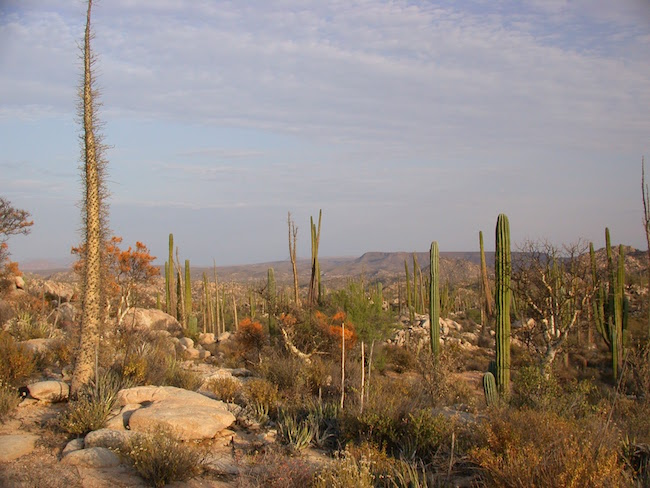
\includegraphics[keepaspectratio]{media/chapter_points.jpg}}

\begin{quote}
Everything is related to everything else, but near things are more
related to each other. Tobler's First Law of Geography\footnote{Pielou
  EC, (1984) The interpretation of ecological data: A primer on
  classification and ordination. 288pg. ISBN:
  \href{https://www.wiley.com/en-us/The+Interpretation+of+Ecological+Data\%3A+A+Primer+on+Classification+and+Ordination-p-9780471889502}{978-0-471-88950-2}}
\end{quote}

\section{Lecture Materials}\label{lecture-materials-8}

\begin{quote}
\textbf{Lecture Slides:} Available interactively in the
\href{https://dyerlabteaching.github.io/Spatial-Points/slides.html\#/title-slide}{online
version}
\end{quote}

\begin{figure}[H]

{\centering \pandocbounded{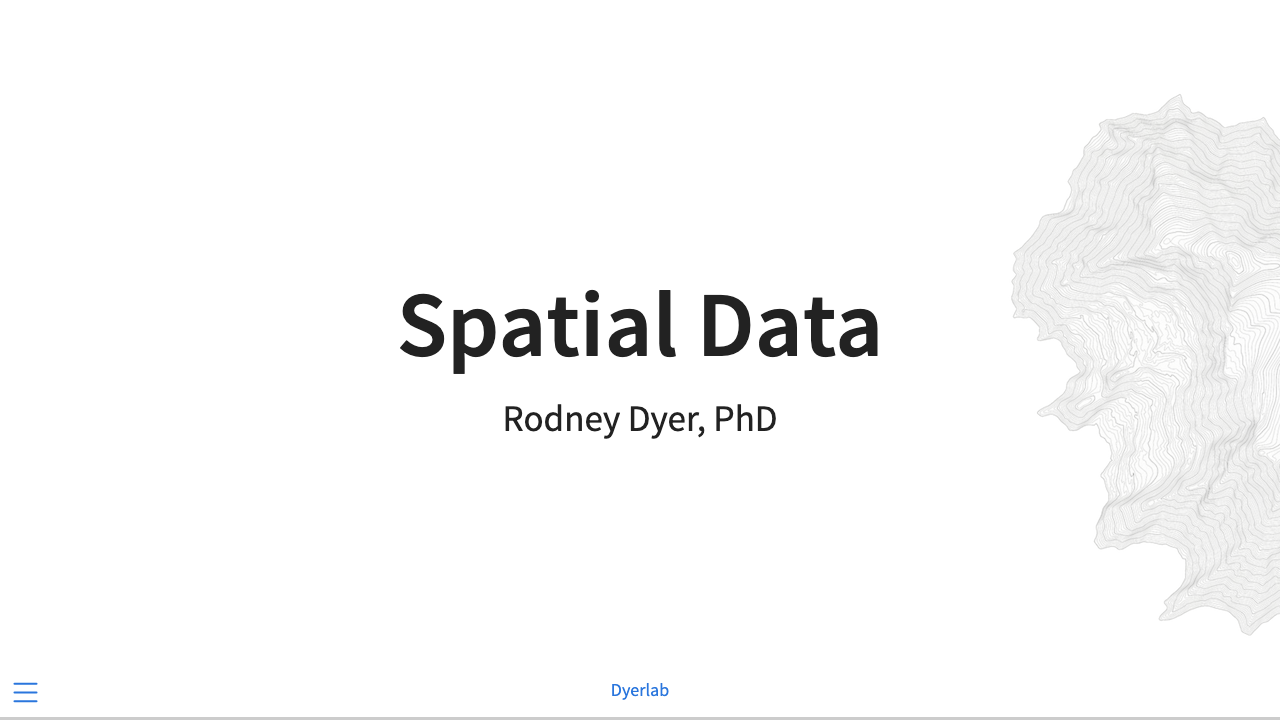
\includegraphics[keepaspectratio]{media/slides_points.png}}

}

\caption{Lecture Slides}

\end{figure}%

Let's start by loading in some of the libraries we'll be using for this
exercise.

\begin{Shaded}
\begin{Highlighting}[]
\FunctionTok{library}\NormalTok{( sf )}
\end{Highlighting}
\end{Shaded}

\begin{verbatim}
Linking to GEOS 3.13.0, GDAL 3.8.5, PROJ 9.5.1; sf_use_s2() is TRUE
\end{verbatim}

\begin{Shaded}
\begin{Highlighting}[]
\FunctionTok{library}\NormalTok{( maps )}
\FunctionTok{library}\NormalTok{( mapproj )}
\FunctionTok{library}\NormalTok{( ggplot2 )}
\FunctionTok{library}\NormalTok{( tidyverse )}
\end{Highlighting}
\end{Shaded}

\begin{verbatim}
-- Attaching core tidyverse packages ------------------------ tidyverse 2.0.0 --
v dplyr     1.2.1     v readr     2.2.0
v forcats   1.0.1     v stringr   1.6.0
v lubridate 1.9.5     v tibble    3.3.1
v purrr     1.2.1     v tidyr     1.3.2
\end{verbatim}

\begin{verbatim}
-- Conflicts ------------------------------------------ tidyverse_conflicts() --
x dplyr::filter() masks stats::filter()
x dplyr::lag()    masks stats::lag()
x purrr::map()    masks maps::map()
i Use the conflicted package (<http://conflicted.r-lib.org/>) to force all conflicts to become errors
\end{verbatim}

\begin{figure}[H]

{\centering \pandocbounded{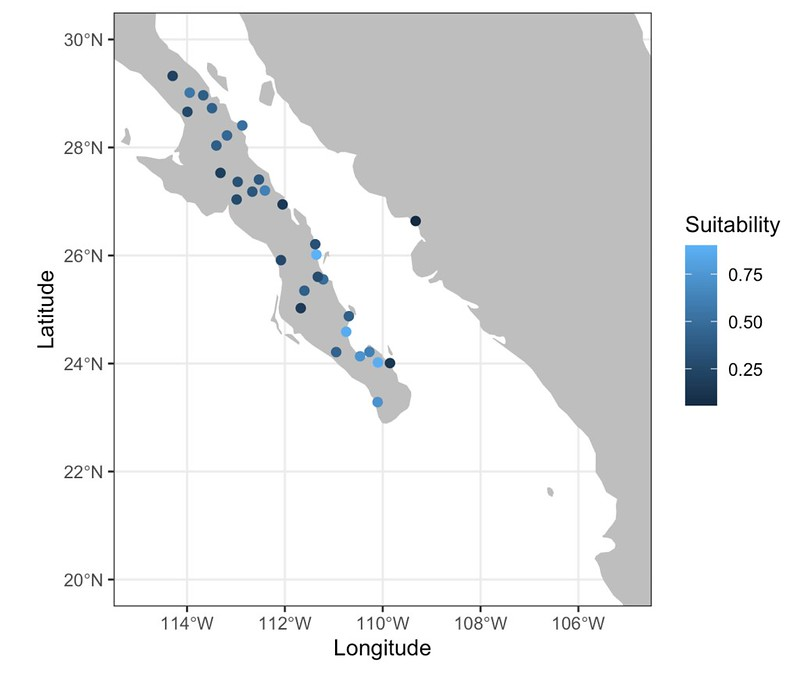
\includegraphics[keepaspectratio]{media/baja_california.jpg}}

}

\caption{Baja California}

\end{figure}%

\section{Learning Objectives}\label{learning-objectives-1}

This topics is the first

\begin{itemize}
\item
  Describe the importance of Ellipsoids \& Datum in spatial data.
\item
  Use both \texttt{sf} \& \texttt{ggplot} in visualizing point data.
\item
  Be able to transform point data from one projection to another.
\end{itemize}

\section{Ellipsoids}\label{ellipsoids}

Unless you are in PHYS 101, the earth is not a perfect sphere (😉). It
is an irregularly shaped object that we need to be able to characterize
if we are going to develop a system of placing points onto it and doing
things such as measuring distance, finding watersheds, or defining
boundaries.

There has been a long history of ellipsoid research, all of which has
been sought to increase our ability to map and move across the earth.
The following table gives some historical and contemporary ellipsoids.

{\def\LTcaptype{none} % do not increment counter
\begin{longtable}[]{@{}
  >{\raggedright\arraybackslash}p{(\linewidth - 6\tabcolsep) * \real{0.1974}}
  >{\centering\arraybackslash}p{(\linewidth - 6\tabcolsep) * \real{0.3026}}
  >{\centering\arraybackslash}p{(\linewidth - 6\tabcolsep) * \real{0.2368}}
  >{\raggedright\arraybackslash}p{(\linewidth - 6\tabcolsep) * \real{0.2632}}@{}}
\toprule\noalign{}
\begin{minipage}[b]{\linewidth}\raggedright
Ellipsoid
\end{minipage} & \begin{minipage}[b]{\linewidth}\centering
Equatorial Radius (m)
\end{minipage} & \begin{minipage}[b]{\linewidth}\centering
Polar Radius (m)
\end{minipage} & \begin{minipage}[b]{\linewidth}\raggedright
Used
\end{minipage} \\
\midrule\noalign{}
\endhead
\bottomrule\noalign{}
\endlastfoot
Maupertuis (1738) & 6,397,300 & 6,363,806.283 & France \\
Plessis (1817) & 6,376,523.0 & 6,355,862.9333 & France \\
Everest (1830) & 6,377,299.365 & 6,356,098.359 & India \\
Everest 1830 Modified (1967) & 6,377,304.063 & 6,356,103.0390 & West
Malaysia \& Singapore \\
Everest 1830 (1967 Definition) & 6,377,298.556 & 6,356,097.550 & Brunei
\& East Malaysia \\
Airy (1830) & 6,377,563.396 & 6,356,256.909 & Britain \\
Bessel (1841) & 6,377,397.155 & 6,356,078.963 & Europe, Japan \\
Clarke (1866) & 6,378,206.4 & 6,356,583.8 & North America \\
Clarke (1878) & 6,378,190 & 6,356,456 & North America \\
Clarke (1880) & 6,378,249.145 & 6,356,514.870 & France, Africa \\
Helmert (1906) & 6,378,200 & 6,356,818.17 & Egypt \\
Hayford (1910) & 6,378,388 & 6,356,911.946 & USA \\
International (1924) & 6,378,388 & 6,356,911.946 & Europe \\
Krassovsky (1940) & 6,378,245 & 6,356,863.019 & USSR, Russia, Romania \\
WGS66 (1966) & 6,378,145 & 6,356,759.769 & USA/DoD \\
Australian National (1966) & 6,378,160 & 6,356,774.719 & Australia \\
New International (1967) & 6,378,157.5 & 6,356,772.2 & \\
GRS-67 (1967) & 6,378,160 & 6,356,774.516 & \\
South American (1969) & 6,378,160 & 6,356,774.719 & South America \\
WGS-72 (1972) & 6,378,135 & 6,356,750.52 & USA/DoD \\
GRS-80 (1979) & 6,378,137 & 6,356,752.3141 & Global ITRS \\
WGS-84 (1984) & 6,378,137 & 6,356,752.3142 & Global GPS \\
IERS (1989) & 6,378,136 & 6,356,751.302 & \\
IERS (2003) & 6,378,136.6 & 6,356,751.9 & \\
\end{longtable}
}

The most common ones you will probably run across include
\texttt{GRS80}/\texttt{NAD83} (derived from satellite measurements of
the distance of the surface to the core of the planet ) and
\texttt{WGS-84} (an ellipsoid based upon GPS).

\subsection{Example Data}\label{example-data}

To examine the differences between ellipsoids, let's load in some data
first. Here are some point data that can be interpreted as polygons and
represent the lower 48 states of the US.

\begin{Shaded}
\begin{Highlighting}[]
\NormalTok{states }\OtherTok{\textless{}{-}} \FunctionTok{map\_data}\NormalTok{(}\StringTok{"state"}\NormalTok{)}
\FunctionTok{head}\NormalTok{( states )}
\end{Highlighting}
\end{Shaded}

\begin{verbatim}
       long      lat group order  region subregion
1 -87.46201 30.38968     1     1 alabama      <NA>
2 -87.48493 30.37249     1     2 alabama      <NA>
3 -87.52503 30.37249     1     3 alabama      <NA>
4 -87.53076 30.33239     1     4 alabama      <NA>
5 -87.57087 30.32665     1     5 alabama      <NA>
6 -87.58806 30.32665     1     6 alabama      <NA>
\end{verbatim}

Each row is a point that is associated with a group (in this case the
state) and is plot in a specific order (to make the outline of the
state). There are 15,537 points required to make the plot, with the
following 49 regions.

\begin{Shaded}
\begin{Highlighting}[]
\FunctionTok{unique}\NormalTok{( states}\SpecialCharTok{$}\NormalTok{region )}
\end{Highlighting}
\end{Shaded}

\begin{verbatim}
 [1] "alabama"              "arizona"              "arkansas"            
 [4] "california"           "colorado"             "connecticut"         
 [7] "delaware"             "district of columbia" "florida"             
[10] "georgia"              "idaho"                "illinois"            
[13] "indiana"              "iowa"                 "kansas"              
[16] "kentucky"             "louisiana"            "maine"               
[19] "maryland"             "massachusetts"        "michigan"            
[22] "minnesota"            "mississippi"          "missouri"            
[25] "montana"              "nebraska"             "nevada"              
[28] "new hampshire"        "new jersey"           "new mexico"          
[31] "new york"             "north carolina"       "north dakota"        
[34] "ohio"                 "oklahoma"             "oregon"              
[37] "pennsylvania"         "rhode island"         "south carolina"      
[40] "south dakota"         "tennessee"            "texas"               
[43] "utah"                 "vermont"              "virginia"            
[46] "washington"           "west virginia"        "wisconsin"           
[49] "wyoming"             
\end{verbatim}

Fortunately for us, our old friend \texttt{ggplot} has a bit of magic
that can do this kind of plotting for us.

\begin{Shaded}
\begin{Highlighting}[]
\FunctionTok{library}\NormalTok{( ggplot2 )}
\FunctionTok{ggplot}\NormalTok{( states, }\FunctionTok{aes}\NormalTok{( }\AttributeTok{x =}\NormalTok{ long, }
                     \AttributeTok{y =}\NormalTok{ lat,}
                     \AttributeTok{group =}\NormalTok{ group ) ) }\SpecialCharTok{+} 
  \FunctionTok{geom\_polygon}\NormalTok{( }\AttributeTok{fill =} \StringTok{"lightgray"}\NormalTok{, }
                \AttributeTok{color =} \StringTok{"black"}\NormalTok{, }
                \AttributeTok{lwd =} \FloatTok{0.25}\NormalTok{) }\SpecialCharTok{+} 
  \FunctionTok{theme\_void}\NormalTok{() }\OtherTok{{-}\textgreater{}}\NormalTok{ p}
\end{Highlighting}
\end{Shaded}

\subsection{Azimuth Projections}\label{azimuth-projections}

An Azimuth Projection is one that is formed by a 2-dimensional plane
that is tangential to the surface of the earth at example one point.
This point may be polar (north or south pole) or oblique (e.g., over
Richmond, Virginia).

\begin{figure}[H]

{\centering \pandocbounded{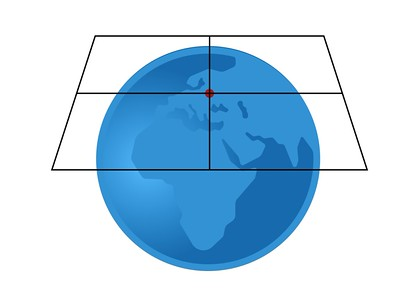
\includegraphics[keepaspectratio]{media/azimuthal_projection.jpg}}

}

\caption{Azequidistant}

\end{figure}%

We can apply different ellipsoids to the map \emph{when we plot it} by
adjusting the coordinate space it is plot within using the
\texttt{coord\_map()} modification. For a whole list of available
projections, see \texttt{?mapproject}.

\begin{Shaded}
\begin{Highlighting}[]
\NormalTok{p }\SpecialCharTok{+} \FunctionTok{coord\_map}\NormalTok{( }\StringTok{"azequalarea"}\NormalTok{)}
\end{Highlighting}
\end{Shaded}

\pandocbounded{
\includegraphics[keepaspectratio]{narrative_points_files/figure-pdf/unnamed-chunk-5-1.pdf}}

\subsection{Cylindrical Projection}\label{cylindrical-projection}

A cylindrical projection is one where a cylinder is wrapped around the
earth creating straight lines for all parallel away from the equator.

\begin{figure}[H]

{\centering \pandocbounded{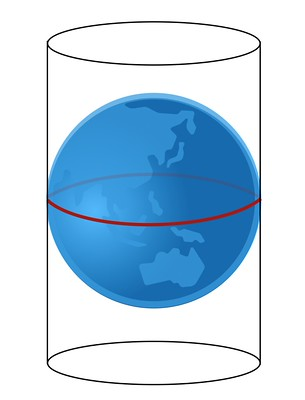
\includegraphics[keepaspectratio]{media/cylindrical_projection.jpg}}

}

\caption{Cylindrical Projection}

\end{figure}%

\begin{Shaded}
\begin{Highlighting}[]
\NormalTok{p }\SpecialCharTok{+} \FunctionTok{coord\_map}\NormalTok{(}\StringTok{"cylindrical"}\NormalTok{)}
\end{Highlighting}
\end{Shaded}

\pandocbounded{
\includegraphics[keepaspectratio]{narrative_points_files/figure-pdf/unnamed-chunk-6-1.pdf}}

\subsection{Conic Projections}\label{conic-projections}

Conic projections are symmetric around the prime meridian and all
parallels are segments of conecntric circles.

\begin{figure}[H]

{\centering \pandocbounded{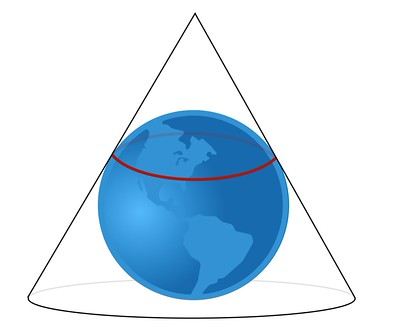
\includegraphics[keepaspectratio]{media/conic_projection.jpg}}

}

\caption{Conic Projection}

\end{figure}%

\begin{Shaded}
\begin{Highlighting}[]
\NormalTok{p }\SpecialCharTok{+} \FunctionTok{coord\_map}\NormalTok{( }\StringTok{"conic"}\NormalTok{, }\AttributeTok{lat0 =} \DecValTok{30}\NormalTok{)}
\end{Highlighting}
\end{Shaded}

\pandocbounded{
\includegraphics[keepaspectratio]{narrative_points_files/figure-pdf/unnamed-chunk-7-1.pdf}}

\section{Datum}\label{datum}

Once we have an ellipsoid model to work with we must define a
\emph{DATUM} type that will represent the coordiante system used. Two
common DATUM types include:

\begin{itemize}
\tightlist
\item
  \emph{Longitude \& Latitude} - The East/West \& North/South position
  on the surface of the earth.

  \begin{itemize}
  \tightlist
  \item
    Prime Meridian (0° Longitude) passes thorugh the
    \href{https://en.wikipedia.org/wiki/Royal_Observatory,_Greenwich}{Royal
    Observatory} in Greenwich England, with positive values of longitude
    to the east and negative to the west.
  \item
    Equator (0° Latitude) and is defined as the point on the planet
    where both northern and southern hemisphers have equal amounts of
    day and night at the
    \href{https://en.wikipedia.org/wiki/Equinox}{equinox} (Sept.~21 \&
    March 21).
  \item
    Richmond, Virginia: 37.533333 Latitude, -77.466667 Longitude
  \end{itemize}
\item
  \emph{Universal Trans Mercator} - A division of the earth into 60
  zones (\textasciitilde6°longitude each, labeled 01 - 60) and 20 bands
  each of which is \textasciitilde8° latitude (labeled C-X excluding I
  \& O with A \& B dividing up Antartica). See image
  \href{https://en.wikipedia.org/wiki/Universal_Transverse_Mercator_coordinate_system\#/media/File:Universal_Transverse_Mercator_zones.svg}{here}.

  \begin{itemize}
  \tightlist
  \item
    Coordinates include Zone \& band designation as well as coordinates
    in Easting and Northing (planar coordinates within the zone)
    measured in meters.
  \item
    Richmond, Virginia: 18S 282051 4156899
  \end{itemize}
\end{itemize}

\begin{tcolorbox}[enhanced jigsaw, arc=.35mm, bottomrule=.15mm, bottomtitle=1mm, breakable, colback=white, colbacktitle=quarto-callout-warning-color!10!white, colframe=quarto-callout-warning-color-frame, coltitle=black, left=2mm, leftrule=.75mm, opacityback=0, opacitybacktitle=0.6, rightrule=.15mm, title=\textcolor{quarto-callout-warning-color}{\faExclamationTriangle}\hspace{0.5em}{Important}, titlerule=0mm, toprule=.15mm, toptitle=1mm]

You \textbf{must} set both the ellipsoid and datum to be \textbf{EXACTLY
THE SAME} for all of your data before you can do any work with it. If
they are not on the same lumpy bumpy planet or in the same coordinate
system, you will be screwed (that is a technical term).

\end{tcolorbox}

\chapter{Defining Projections}\label{defining-projections}

Projections are a combination of the underlying elipse as well as the
definition of the datum. There are literally thousands of recognized
projections, each of which has to be able to be sufficiently defined
such that we can convert from one recognized projection to
another\footnote{You should be careful when you use joins on \texttt{sf}
  objects. If you \texttt{sf} object is on the right side (see
  discussion of joins
  \href{https://dyerlab.github.io/ENVS-Lectures/manipulation/relational_data/slides.html\#5}{here})
  then the result will not be an \texttt{sf} object and you'll have to
  coerce it back into one again. It always adopts the characteristics of
  the left object.}.

One of the repositories for these projections can be found at
\href{https://epsg.io}{epsg.io}.

\begin{figure}[H]

{\centering \pandocbounded{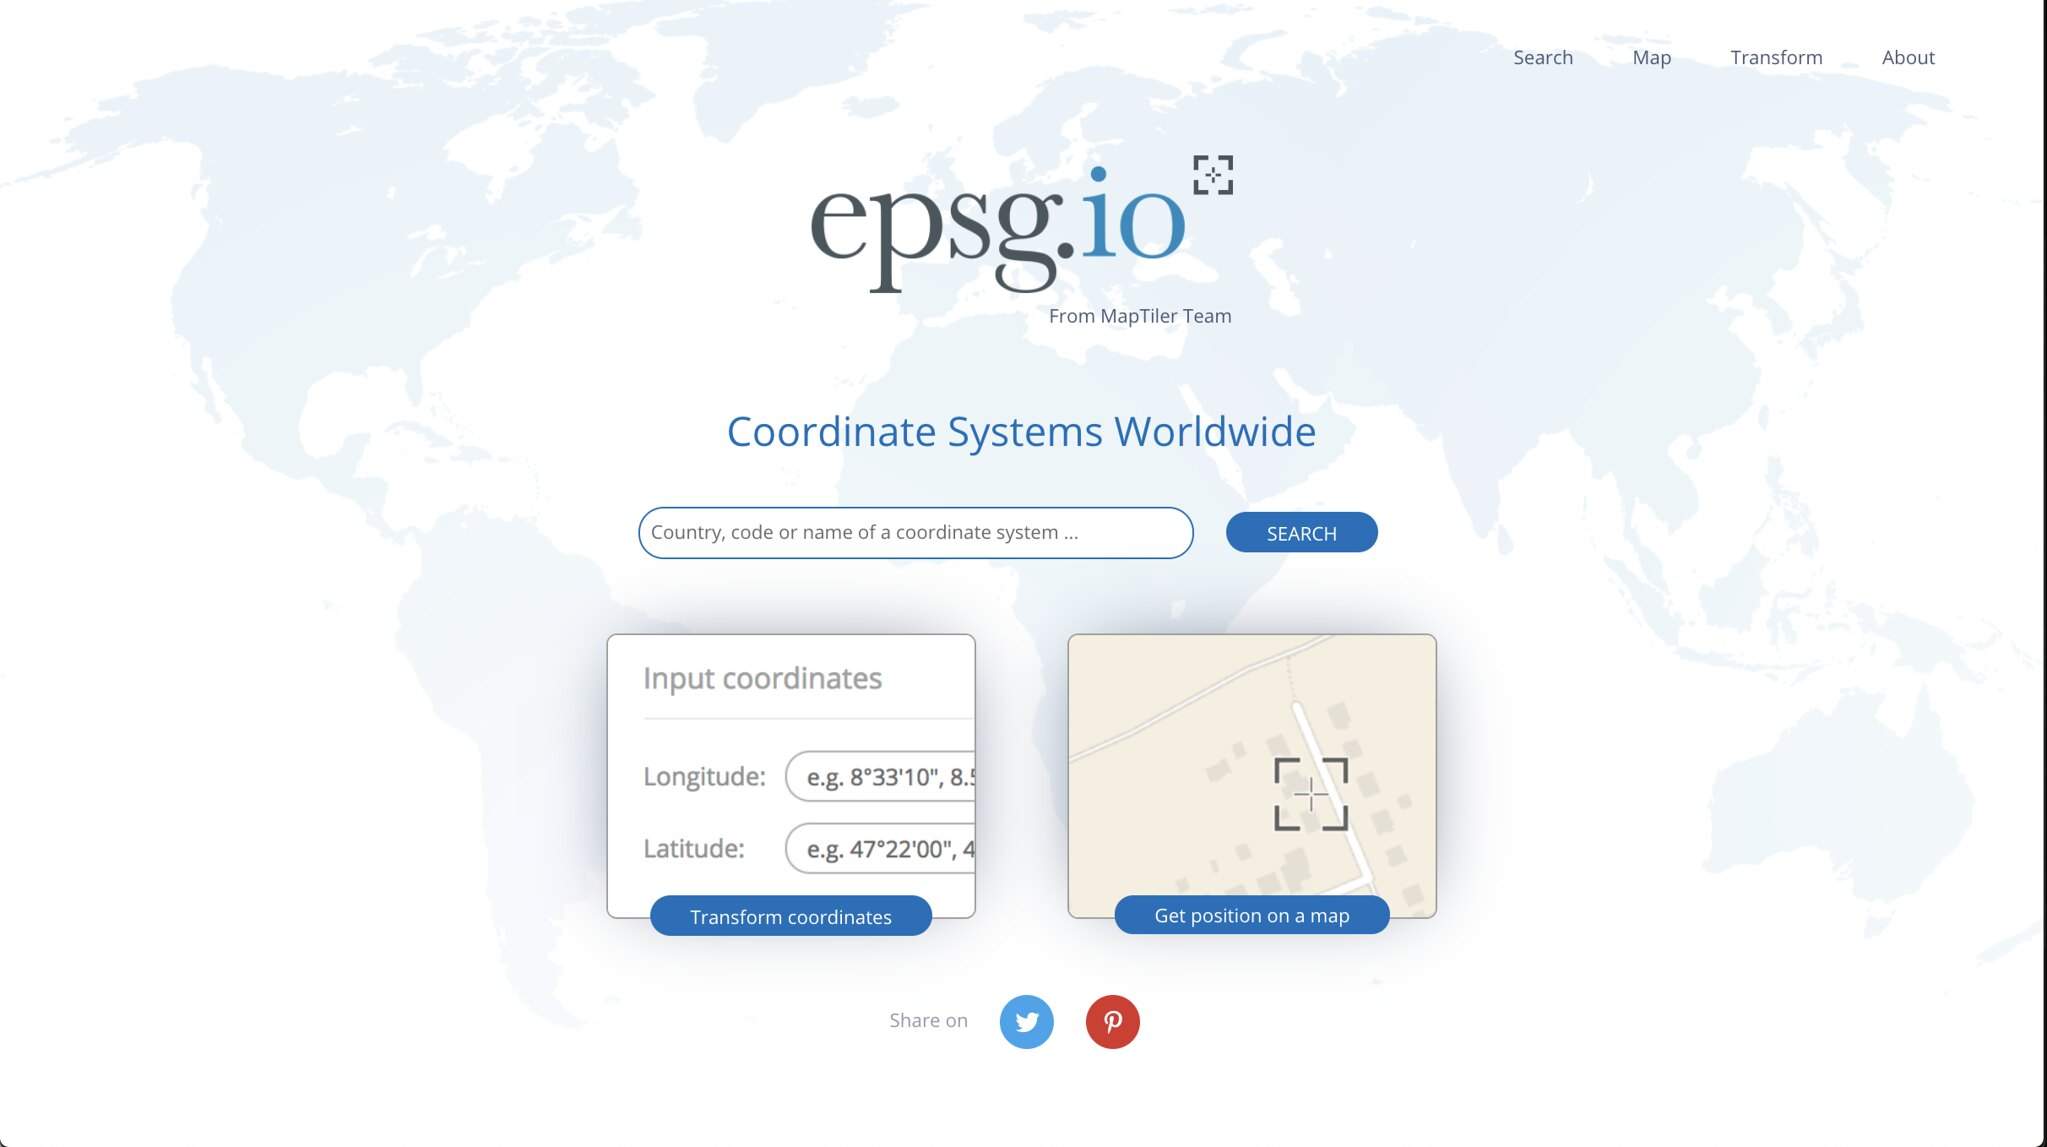
\includegraphics[keepaspectratio]{media/epsg_io.jpg}}

}

\caption{epsg.io}

\end{figure}%

The EPSG Geodetic Parameter Dataset (also known as the EPGS\footnote{The
  EPSG standard was originally created in 1985 by the
  \href{European\%20Petroleum\%20Survey\%20Group}{https://en.wikipedia.org/wiki/European\_Petroleum\_Survey\_Group}
  and made public in 1993.} registry) is a publc registry of datums,
spatial reference systems, and earth elipsoids. Each item is assigned a
specific EPSG code

The precise definitions of projections come in several different
formats, some of which include:

Well Known Text (WKT)

\begin{verbatim}
GEOGCS["WGS 84",
    DATUM["WGS_1984",
        SPHEROID["WGS 84",6378137,298.257223563,
            AUTHORITY["EPSG","7030"]],
        AUTHORITY["EPSG","6326"]],
    PRIMEM["Greenwich",0,
        AUTHORITY["EPSG","8901"]],
    UNIT["degree",0.0174532925199433,
        AUTHORITY["EPSG","9122"]],
    AUTHORITY["EPSG","4326"]]
\end{verbatim}

PROJ.4

\begin{verbatim}
+proj=longlat +datum=WGS84 +no_defs 
\end{verbatim}

If you work with ESRI software, when you have a projected shapefile, one
of the several files that go with that shapefile is the \texttt{.prj}
file which will contain the ESRI WKT below.

\begin{verbatim}
GEOGCS["GCS_WGS_1984",DATUM["D_WGS_1984",SPHEROID["WGS_1984",6378137,298.257223563]],PRIMEM["Greenwich",0],UNIT["Degree",0.017453292519943295]]
\end{verbatim}

\begin{tcolorbox}[enhanced jigsaw, arc=.35mm, bottomrule=.15mm, bottomtitle=1mm, breakable, colback=white, colbacktitle=quarto-callout-tip-color!10!white, colframe=quarto-callout-tip-color-frame, coltitle=black, left=2mm, leftrule=.75mm, opacityback=0, opacitybacktitle=0.6, rightrule=.15mm, title=\textcolor{quarto-callout-tip-color}{\faLightbulb}\hspace{0.5em}{Best Practice}, titlerule=0mm, toprule=.15mm, toptitle=1mm]

Always let the underlying software make any changes to projection
information. There is a lot of difficult conversions that need to happen
to reproject from one CRS to another.

\end{tcolorbox}

\chapter{Point Data}\label{point-data-1}

To start off, we will load in some data from the bark beetle,
\emph{Araptus attenuatus}, a Sonoran Desert endemic parasite that lives
within the plant \emph{Euphorbia lomelii}.

\begin{figure}

\begin{minipage}[t]{0.50\linewidth}

\begin{figure}[H]

{\centering \pandocbounded{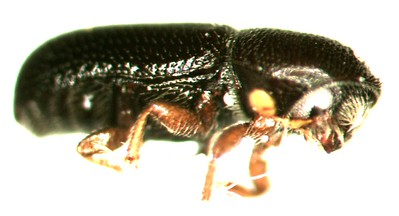
\includegraphics[keepaspectratio]{media/araptus_attenuatus.jpg}}

}

\subcaption{Araptus attenuatus}

\end{figure}%

\end{minipage}%
%
\begin{minipage}[t]{0.50\linewidth}

\begin{figure}[H]

{\centering \pandocbounded{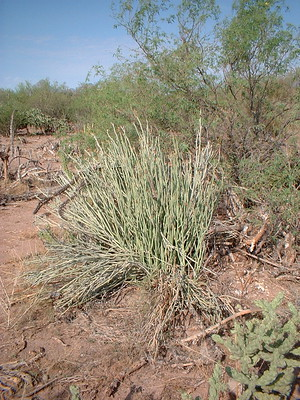
\includegraphics[keepaspectratio]{media/euphorbia_lomelii.jpg}}

}

\subcaption{Euphorbia lomelii}

\end{figure}%

\end{minipage}%

\end{figure}%

As part of some work that we have done on these species, we have looked
at the relationship between habitat suitability and sex ratio bias. The
life history for this beetle is such that males will establish home by
burrowing in the senescing tissues of the host plant. Once established,
feamles are attracted via phermones.

\begin{Shaded}
\begin{Highlighting}[]
\NormalTok{url }\OtherTok{\textless{}{-}} \StringTok{"https://raw.githubusercontent.com/dyerlab/ENVS{-}Lectures/master/data/Araptus\_Disperal\_Bias.csv"}
\FunctionTok{read\_csv}\NormalTok{( url ) }\SpecialCharTok{|\textgreater{}}
  \FunctionTok{select}\NormalTok{( Site, Longitude, Latitude, }\FunctionTok{everything}\NormalTok{() ) }\SpecialCharTok{|\textgreater{}}
  \FunctionTok{arrange}\NormalTok{( Latitude ) }\OtherTok{{-}\textgreater{}}\NormalTok{ data }
\end{Highlighting}
\end{Shaded}

\begin{verbatim}
Rows: 31 Columns: 9
-- Column specification --------------------------------------------------------
Delimiter: ","
chr (1): Site
dbl (8): Males, Females, Suitability, MFRatio, GenVarArapat, GenVarEuphli, L...

i Use `spec()` to retrieve the full column specification for this data.
i Specify the column types or set `show_col_types = FALSE` to quiet this message.
\end{verbatim}

\begin{Shaded}
\begin{Highlighting}[]
\FunctionTok{summary}\NormalTok{( data )}
\end{Highlighting}
\end{Shaded}

\begin{verbatim}
     Site             Longitude         Latitude         Males      
 Length:31          Min.   :-114.3   Min.   :23.29   Min.   : 9.00  
 Class :character   1st Qu.:-113.1   1st Qu.:24.95   1st Qu.:16.00  
 Mode  :character   Median :-112.0   Median :26.64   Median :21.00  
                    Mean   :-112.0   Mean   :26.44   Mean   :25.68  
                    3rd Qu.:-110.8   3rd Qu.:27.78   3rd Qu.:31.50  
                    Max.   :-109.3   Max.   :29.33   Max.   :64.00  
    Females       Suitability        MFRatio        GenVarArapat   
 Min.   : 5.00   Min.   :0.0563   Min.   :0.5938   Min.   :0.0500  
 1st Qu.:15.50   1st Qu.:0.2732   1st Qu.:0.8778   1st Qu.:0.1392  
 Median :21.00   Median :0.3975   Median :1.1200   Median :0.2002  
 Mean   :23.52   Mean   :0.4276   Mean   :1.1598   Mean   :0.2006  
 3rd Qu.:29.00   3rd Qu.:0.5442   3rd Qu.:1.3618   3rd Qu.:0.2592  
 Max.   :63.00   Max.   :0.9019   Max.   :2.2000   Max.   :0.3379  
  GenVarEuphli   
 Min.   :0.0500  
 1st Qu.:0.1777  
 Median :0.2171  
 Mean   :0.2203  
 3rd Qu.:0.2517  
 Max.   :0.5122  
\end{verbatim}

We can plot these points using the normal \texttt{ggplot} functions (map
overlays below).

\begin{Shaded}
\begin{Highlighting}[]
\FunctionTok{library}\NormalTok{(ggrepel)}
\NormalTok{data }\SpecialCharTok{|\textgreater{}}
  \FunctionTok{ggplot}\NormalTok{( }\FunctionTok{aes}\NormalTok{( Longitude, Latitude ) ) }\SpecialCharTok{+} 
  \FunctionTok{geom\_label\_repel}\NormalTok{( }\FunctionTok{aes}\NormalTok{(}\AttributeTok{label=}\NormalTok{Site) ) }\SpecialCharTok{+} 
  \FunctionTok{coord\_map}\NormalTok{()}
\end{Highlighting}
\end{Shaded}

\pandocbounded{
\includegraphics[keepaspectratio]{narrative_points_files/figure-pdf/unnamed-chunk-9-1.pdf}}

We can also plot these locations and fill in some interpretive data
using the \texttt{leaflet} library to create an interactive map as
follows:

\begin{figure}[H]

{\centering \pandocbounded{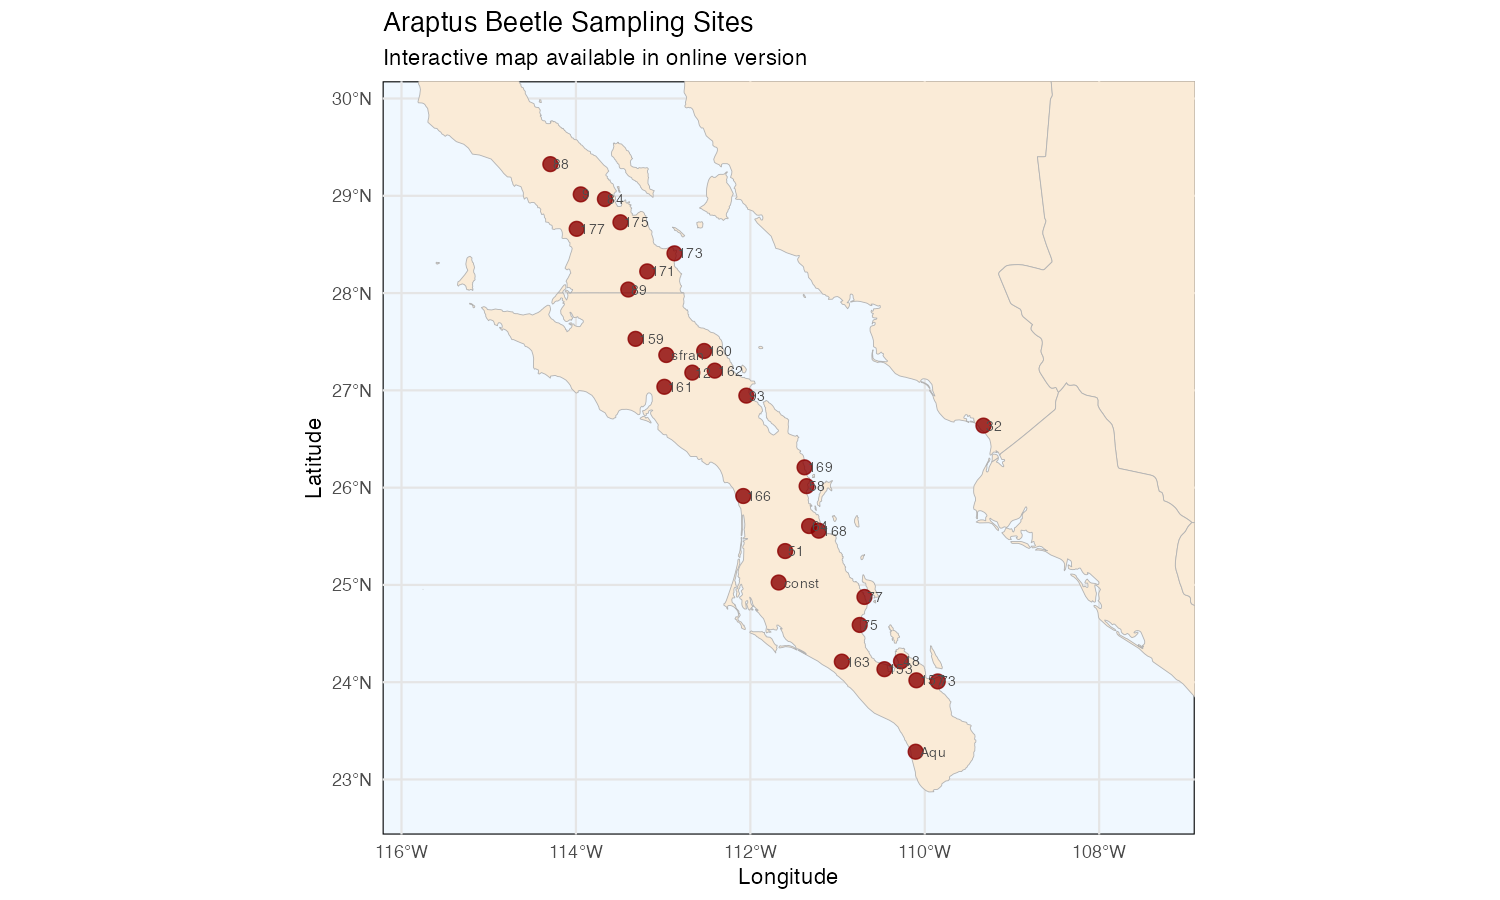
\includegraphics[keepaspectratio]{media/map_points_leaflet.png}}

}

\caption{Araptus Beetle Sampling Sites - Interactive map available in
online version}

\end{figure}%

In this case, we are using the latitude and longitude as numerical
values of which the \texttt{leaflet} library is able to intrepret
properly. However, just like we did for
\href{https://dyerlab.github.io/ENVS-Lectures/r_language/dates/slides.html\#1}{date-like
data}, we can convert these into a geographically relevant data type
that knows a lot about geospatial processes rather than keeping it as a
numeric value that we ``assume'' will work properly. For this we will
use the \texttt{sf} library.

\section{\texorpdfstring{\texttt{sf}
Objects}{sf Objects}}\label{sf-objects}

\emph{Simple Features} (hereafter abbreviated as \texttt{sf}) are an
open standard developed by the Open Geospatial Consortium
(\href{https://ogc.org}{OGC}). They define the following basic types:

\begin{itemize}
\tightlist
\item
  POINT\\
\item
  LINESTRING
\item
  POLYGON\\
\item
  MULTIPOINT
\item
  MULTILINESTRING
\item
  MULTIPOLYGON
\item
  GEOMETRYCOLLECTION
\end{itemize}

Each of these basic types can be represented within a single column of a
\texttt{data.frame}. To do this, we need to tell the conversion function
\texttt{st\_as\_sf()} which columns to consider as the datum and which
ellipsoid to use.

\begin{Shaded}
\begin{Highlighting}[]
\FunctionTok{library}\NormalTok{( sf )}
\NormalTok{data }\SpecialCharTok{|\textgreater{}}
  \FunctionTok{st\_as\_sf}\NormalTok{( }\AttributeTok{coords=}\FunctionTok{c}\NormalTok{(}\StringTok{"Longitude"}\NormalTok{,}\StringTok{"Latitude"}\NormalTok{),}
            \AttributeTok{crs =} \DecValTok{4326}\NormalTok{ ) }\OtherTok{{-}\textgreater{}}\NormalTok{ data}
\FunctionTok{head}\NormalTok{( data )}
\end{Highlighting}
\end{Shaded}

\begin{verbatim}
Simple feature collection with 6 features and 7 fields
Geometry type: POINT
Dimension:     XY
Bounding box:  xmin: -110.951 ymin: 23.2855 xmax: -109.8507 ymax: 24.21441
Geodetic CRS:  WGS 84
# A tibble: 6 x 8
  Site  Males Females Suitability MFRatio GenVarArapat GenVarEuphli
  <chr> <dbl>   <dbl>       <dbl>   <dbl>        <dbl>        <dbl>
1 Aqu      12       9       0.722   1.33         0.120       0.0968
2 73       11       5       0.146   2.2          0.137       0.253 
3 157      26      30       0.881   0.867        0.150       0.191 
4 153      35      41       0.732   0.854        0.333       0.276 
5 163      21      21       0.433   1            0.298       0.338 
6 48       18      27       0.620   0.667        0.115       0.213 
# i 1 more variable: geometry <POINT [°]>
\end{verbatim}

This conversion to an \texttt{sf} object adds attributes to the
\texttt{data.frame} and \texttt{tibble} object.

\begin{Shaded}
\begin{Highlighting}[]
\FunctionTok{class}\NormalTok{( data )}
\end{Highlighting}
\end{Shaded}

\begin{verbatim}
[1] "sf"         "tbl_df"     "tbl"        "data.frame"
\end{verbatim}

This additional \texttt{sf} attributes gives it more qualities such as a
bounding box (e.g., the area within which all the poitns exist)

\begin{Shaded}
\begin{Highlighting}[]
\FunctionTok{st\_bbox}\NormalTok{( data )}
\end{Highlighting}
\end{Shaded}

\begin{verbatim}
      xmin       ymin       xmax       ymax 
-114.29353   23.28550 -109.32700   29.32541 
\end{verbatim}

Distances between objects.

\begin{Shaded}
\begin{Highlighting}[]
\FunctionTok{st\_distance}\NormalTok{( data[}\DecValTok{1}\NormalTok{,], data[}\DecValTok{2}\NormalTok{,])}
\end{Highlighting}
\end{Shaded}

\begin{verbatim}
Units: [m]
        [,1]
[1,] 84376.8
\end{verbatim}

As well as complex geospatial operations such as finding the convex hull
(the minimal area containing all poitns).

\begin{Shaded}
\begin{Highlighting}[]
\NormalTok{data }\SpecialCharTok{|\textgreater{}}
  \FunctionTok{st\_union}\NormalTok{() }\SpecialCharTok{|\textgreater{}}
  \FunctionTok{st\_convex\_hull}\NormalTok{() }\OtherTok{{-}\textgreater{}}\NormalTok{ hull}
\NormalTok{hull}
\end{Highlighting}
\end{Shaded}

\begin{verbatim}
Geometry set for 1 feature 
Geometry type: POLYGON
Dimension:     XY
Bounding box:  xmin: -114.2935 ymin: 23.2855 xmax: -109.327 ymax: 29.32541
Geodetic CRS:  WGS 84
\end{verbatim}

\begin{verbatim}
POLYGON ((-114.2935 29.32541, -113.9914 28.6605...
\end{verbatim}

the center of the all the points.

\begin{Shaded}
\begin{Highlighting}[]
\NormalTok{hull }\SpecialCharTok{|\textgreater{}}
  \FunctionTok{st\_centroid}\NormalTok{()}
\end{Highlighting}
\end{Shaded}

\begin{verbatim}
Geometry set for 1 feature 
Geometry type: POINT
Dimension:     XY
Bounding box:  xmin: -111.3417 ymin: 26.37741 xmax: -111.3417 ymax: 26.37741
Geodetic CRS:  WGS 84
\end{verbatim}

\begin{verbatim}
POINT (-111.3417 26.37741)
\end{verbatim}

and the area enclosed by all the points (for various units).

\begin{Shaded}
\begin{Highlighting}[]
\FunctionTok{library}\NormalTok{( units )}
\end{Highlighting}
\end{Shaded}

\begin{verbatim}
udunits database from /Library/Frameworks/R.framework/Versions/4.5-arm64/Resources/library/units/share/udunits/udunits2.xml
\end{verbatim}

\begin{Shaded}
\begin{Highlighting}[]
\NormalTok{hull }\SpecialCharTok{|\textgreater{}}
  \FunctionTok{st\_area}\NormalTok{() }\SpecialCharTok{|\textgreater{}}
  \FunctionTok{set\_units}\NormalTok{( km}\SpecialCharTok{\^{}}\DecValTok{2}\NormalTok{ )}
\end{Highlighting}
\end{Shaded}

\begin{verbatim}
122130.5 [km^2]
\end{verbatim}

\subsection{Reprojecting}\label{reprojecting}

In addition to the operations above, properly created \texttt{sf}
objects can easily be projected from one CRS into another (epsg 6372 is
a common projection covering Mexico based upon the GRS80 elipsoid and
the latest ITRF2008 datum standard based on the meter)\footnote{This
  standard is defined by \href{https://www.inegi.org.mx}{Sistema
  Nacional de Información Estadística y Geográfica}.}.

\begin{Shaded}
\begin{Highlighting}[]
\NormalTok{data }\SpecialCharTok{|\textgreater{}}
  \FunctionTok{st\_transform}\NormalTok{( }\DecValTok{6372}\NormalTok{ ) }\SpecialCharTok{|\textgreater{}}
  \FunctionTok{st\_bbox}\NormalTok{()}
\end{Highlighting}
\end{Shaded}

\begin{verbatim}
   xmin    ymin    xmax    ymax 
1307745 1274010 1773676 1968473 
\end{verbatim}

Again, do this \textbf{first} to all your data to make sure it is put
into a proper projection (and most of your headaches will disappear).

\subsection{\texorpdfstring{Plotting \texttt{sf}
Objects}{Plotting sf Objects}}\label{plotting-sf-objects}

Analogous to the duality between built-in \texttt{R} plotting and
\texttt{ggplot} approaches, we can use either of these frameworks to
plot \texttt{sf} objects.

As built-in objects, a \texttt{sf} data set that has a geometry
coordinate is intrinsically linked to all the other data columns. If we
plot the entire data frame, we see that for each non-geometry data
column, we create an individual plot.

\begin{Shaded}
\begin{Highlighting}[]
\FunctionTok{plot}\NormalTok{( data )}
\end{Highlighting}
\end{Shaded}

\pandocbounded{
\includegraphics[keepaspectratio]{narrative_points_files/figure-pdf/unnamed-chunk-19-1.pdf}}

The data with the \texttt{data.frame} can be accessed as normal.

\begin{Shaded}
\begin{Highlighting}[]
\FunctionTok{plot}\NormalTok{( data}\SpecialCharTok{$}\NormalTok{Suitability )}
\end{Highlighting}
\end{Shaded}

\pandocbounded{
\includegraphics[keepaspectratio]{narrative_points_files/figure-pdf/unnamed-chunk-20-1.pdf}}

But if we plot it using the square brackets and names of dat columns, we
can link the \texttt{geometry} column to it and plot it as a spatial
representation of those data (and adorn it with the normal
\texttt{plot()} upgrades accordingly).

\begin{Shaded}
\begin{Highlighting}[]
\FunctionTok{plot}\NormalTok{( data[}\StringTok{"Suitability"}\NormalTok{], }\AttributeTok{pch=}\DecValTok{16}\NormalTok{, }\AttributeTok{cex=}\DecValTok{2}\NormalTok{)}
\end{Highlighting}
\end{Shaded}

\pandocbounded{
\includegraphics[keepaspectratio]{narrative_points_files/figure-pdf/unnamed-chunk-21-1.pdf}}

Perhaps not surprisingly, \texttt{ggplot()} also works the same way,
however, the geospatial coordiantes for the plot aare taken care of
using \texttt{geom\_sf()} and you are left with definining which of the
data columns you want to put into the plot as a component of the
\texttt{aes()} definition.

\begin{Shaded}
\begin{Highlighting}[]
\FunctionTok{ggplot}\NormalTok{( data, }\FunctionTok{aes}\NormalTok{(}\AttributeTok{color=}\NormalTok{Suitability) ) }\SpecialCharTok{+} 
  \FunctionTok{geom\_sf}\NormalTok{( )}
\end{Highlighting}
\end{Shaded}

\pandocbounded{
\includegraphics[keepaspectratio]{narrative_points_files/figure-pdf/unnamed-chunk-22-1.pdf}}

It works the same ways for lables.

\begin{Shaded}
\begin{Highlighting}[]
\FunctionTok{ggplot}\NormalTok{( data ) }\SpecialCharTok{+} 
  \FunctionTok{geom\_sf\_text}\NormalTok{( }\FunctionTok{aes}\NormalTok{(}\AttributeTok{label=}\NormalTok{Site) ) }\SpecialCharTok{+} 
  \FunctionTok{theme\_void}\NormalTok{() }\SpecialCharTok{+} 
  \FunctionTok{coord\_map}\NormalTok{()}
\end{Highlighting}
\end{Shaded}

\begin{verbatim}
Warning in st_point_on_surface.sfc(sf::st_zm(x)): st_point_on_surface may not
give correct results for longitude/latitude data
\end{verbatim}

\pandocbounded{
\includegraphics[keepaspectratio]{narrative_points_files/figure-pdf/unnamed-chunk-23-1.pdf}}

\chapter{Map Overlays}\label{map-overlays}

We can go out and grab a map background to overlay these plots onto,
giving more context (similiarly to how we did this above using leaflet).

The \texttt{map\_data()} function is part of \texttt{ggplot()} and
produces a \texttt{data.frame} object where each row is a coordinate
used to draw polygons (see
\href{https://dyerlab.github.io/ENVS-Lectures/spatial/spatial_polygons/narrative.nb.html}{narrative}
on polygons for more information).

\begin{Shaded}
\begin{Highlighting}[]
\FunctionTok{map\_data}\NormalTok{(}\StringTok{"world"}\NormalTok{) }\SpecialCharTok{|\textgreater{}}
  \FunctionTok{filter}\NormalTok{( region }\SpecialCharTok{==} \StringTok{"Mexico"}\NormalTok{) }\OtherTok{{-}\textgreater{}}\NormalTok{ map}
\FunctionTok{head}\NormalTok{( map )}
\end{Highlighting}
\end{Shaded}

\begin{verbatim}
       long      lat group order region       subregion
1 -91.68369 18.67734   970 60731 Mexico Isla del Carmen
2 -91.79614 18.65420   970 60732 Mexico Isla del Carmen
3 -91.81612 18.67588   970 60733 Mexico Isla del Carmen
4 -91.58911 18.77803   970 60734 Mexico Isla del Carmen
5 -91.55029 18.77368   970 60735 Mexico Isla del Carmen
6 -91.53672 18.76001   970 60736 Mexico Isla del Carmen
\end{verbatim}

In \texttt{ggplot} there is a \texttt{geom\_polygon()} function that
takes these series of coordiantes and draws them properly over which we
can lay down the \texttt{sf} object.

However, notice that the boundary boxes for the data and the map are
vastly different (the underlying map is much bigger).

\begin{Shaded}
\begin{Highlighting}[]
\FunctionTok{cbind}\NormalTok{( }\AttributeTok{Data =} \FunctionTok{st\_bbox}\NormalTok{( data ), }\AttributeTok{Map =} \FunctionTok{c}\NormalTok{(}\FunctionTok{min}\NormalTok{(map}\SpecialCharTok{$}\NormalTok{long), }\FunctionTok{min}\NormalTok{(map}\SpecialCharTok{$}\NormalTok{lat), }\FunctionTok{max}\NormalTok{(map}\SpecialCharTok{$}\NormalTok{long), }\FunctionTok{max}\NormalTok{(map}\SpecialCharTok{$}\NormalTok{lat) ) )}
\end{Highlighting}
\end{Shaded}

\begin{verbatim}
           Data        Map
xmin -114.29353 -118.40137
ymin   23.28550   14.54541
xmax -109.32700  -86.69629
ymax   29.32541   32.71533
\end{verbatim}

So if we plot it as is, we have points only in a small area of the plot.

\begin{Shaded}
\begin{Highlighting}[]
\FunctionTok{ggplot}\NormalTok{( ) }\SpecialCharTok{+} 
  \FunctionTok{geom\_polygon}\NormalTok{( }\FunctionTok{aes}\NormalTok{( }\AttributeTok{x=}\NormalTok{long, }
                     \AttributeTok{y=}\NormalTok{lat, }
                     \AttributeTok{group=}\NormalTok{group ), }
                \AttributeTok{data=}\NormalTok{map, }
                \AttributeTok{fill=}\StringTok{"grey"}\NormalTok{ ) }\SpecialCharTok{+} 
  \FunctionTok{geom\_sf}\NormalTok{( }\AttributeTok{data=}\NormalTok{data, }
           \FunctionTok{aes}\NormalTok{(}\AttributeTok{color=}\NormalTok{Suitability), }
           \AttributeTok{size=}\DecValTok{2}\NormalTok{) }\SpecialCharTok{+}
  \FunctionTok{xlab}\NormalTok{(}\StringTok{"Longitude"}\NormalTok{) }\SpecialCharTok{+} 
  \FunctionTok{ylab}\NormalTok{(}\StringTok{"Latitude"}\NormalTok{) }\SpecialCharTok{+} 
  \FunctionTok{theme\_bw}\NormalTok{( }\AttributeTok{base\_size =} \DecValTok{12}\NormalTok{ ) }
\end{Highlighting}
\end{Shaded}

\pandocbounded{
\includegraphics[keepaspectratio]{narrative_points_files/figure-pdf/unnamed-chunk-26-1.pdf}}

In a normal \texttt{ggplot()} display we could use
\texttt{+\ xlim()\ +\ ylim()} but since we are combining both
\texttt{geom\_polygon} and \texttt{geom\_sf}, we are required to do this
in the \texttt{coord\_sf()} function to make it work
correctly\footnote{This is because if we use the normal procedures, we
  mess up the order in which everything is plot in
  \texttt{geom\_polygon()}, try it and see.}.

\begin{Shaded}
\begin{Highlighting}[]
\FunctionTok{ggplot}\NormalTok{( ) }\SpecialCharTok{+} 
  \FunctionTok{geom\_polygon}\NormalTok{( }\FunctionTok{aes}\NormalTok{( }\AttributeTok{x=}\NormalTok{long, }
                     \AttributeTok{y=}\NormalTok{lat, }
                     \AttributeTok{group=}\NormalTok{group ), }
                \AttributeTok{data=}\NormalTok{map, }
                \AttributeTok{fill=}\StringTok{"grey"}\NormalTok{ ) }\SpecialCharTok{+} 
  \FunctionTok{geom\_sf}\NormalTok{( }\AttributeTok{data=}\NormalTok{data, }
           \FunctionTok{aes}\NormalTok{(}\AttributeTok{color=}\NormalTok{Suitability), }
           \AttributeTok{size=}\DecValTok{2}\NormalTok{) }\SpecialCharTok{+}
  \FunctionTok{xlab}\NormalTok{(}\StringTok{"Longitude"}\NormalTok{) }\SpecialCharTok{+} 
  \FunctionTok{ylab}\NormalTok{(}\StringTok{"Latitude"}\NormalTok{) }\SpecialCharTok{+} 
  \FunctionTok{theme\_bw}\NormalTok{( }\AttributeTok{base\_size =} \DecValTok{12}\NormalTok{ ) }\SpecialCharTok{+}
  \FunctionTok{coord\_sf}\NormalTok{( }\AttributeTok{xlim =} \FunctionTok{c}\NormalTok{(}\SpecialCharTok{{-}}\DecValTok{115}\NormalTok{, }\SpecialCharTok{{-}}\DecValTok{105}\NormalTok{),}
            \AttributeTok{ylim =} \FunctionTok{c}\NormalTok{(}\DecValTok{20}\NormalTok{, }\DecValTok{30}\NormalTok{) )}
\end{Highlighting}
\end{Shaded}

\pandocbounded{
\includegraphics[keepaspectratio]{narrative_points_files/figure-pdf/unnamed-chunk-27-1.pdf}}

\chapter{Vector Data}\label{vector-data}

\pandocbounded{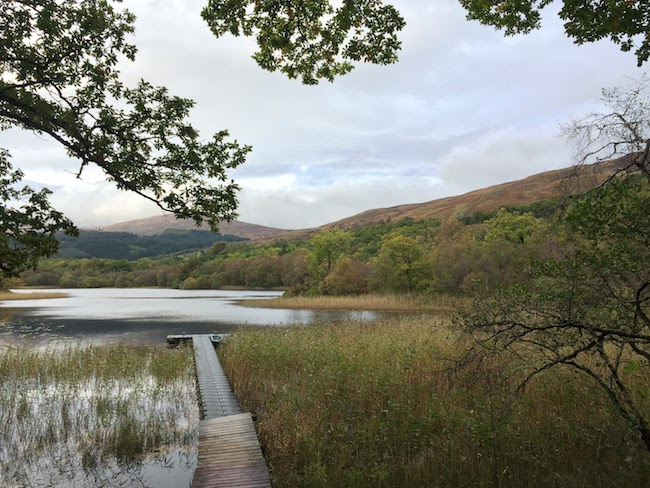
\includegraphics[keepaspectratio]{media/chapter_vector.jpg}}

\begin{quote}
Connecting points creates more complicated data types---vector
data---that represent lines and polygons.
\end{quote}

In this topic, we will focus on lines and polygons. These are
represented as \texttt{sf} objects, we can leverage a large amount of
\texttt{st\_*} functions to perform manipulations, and we can visualize
them using either built-in routines or via \texttt{ggplot} (as
expected).

\section{Lecture Materials}\label{lecture-materials-9}

\begin{quote}
\textbf{Lecture Slides:} Available interactively in the
\href{https://dyerlabteaching.github.io/Shapefiles/slides.html\#/title-slide}{online
version}
\end{quote}

\begin{figure}[H]

{\centering \pandocbounded{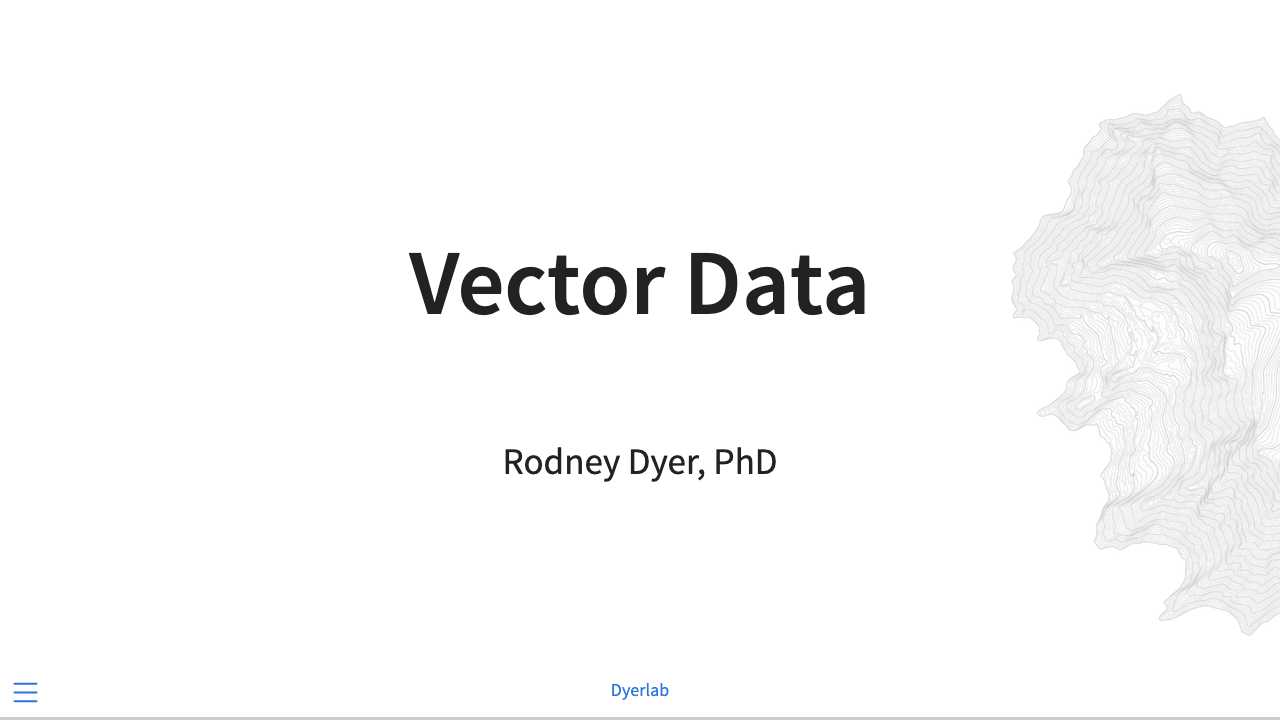
\includegraphics[keepaspectratio]{media/slides_vector.png}}

}

\caption{Lecture Slides}

\end{figure}%

\section{Raw Data}\label{raw-data}

The data for this are going to be represented by roads and development
zones in Richmond, Virginia. These data are made available by the GIS
Department of the City of Richmond. For this example, we will be loading
these in as \emph{shapefiles}.

You can load in shapefile data directly into R but we have to do a
little work. First, we should understand that \emph{a shapefile} is not
an actual file, it is a collection of several files. They are often
zipped up into a single archive.

Here are two shape file archives that I have up on Github in the class
repository.

\begin{Shaded}
\begin{Highlighting}[]
\FunctionTok{library}\NormalTok{( sf )}
\end{Highlighting}
\end{Shaded}

\begin{verbatim}
Linking to GEOS 3.13.0, GDAL 3.8.5, PROJ 9.5.1; sf_use_s2() is TRUE
\end{verbatim}

\begin{Shaded}
\begin{Highlighting}[]
\FunctionTok{library}\NormalTok{( tidyverse )}
\end{Highlighting}
\end{Shaded}

\begin{verbatim}
-- Attaching core tidyverse packages ------------------------ tidyverse 2.0.0 --
v dplyr     1.2.1     v readr     2.2.0
v forcats   1.0.1     v stringr   1.6.0
v ggplot2   4.0.2     v tibble    3.3.1
v lubridate 1.9.5     v tidyr     1.3.2
v purrr     1.2.1     
\end{verbatim}

\begin{verbatim}
-- Conflicts ------------------------------------------ tidyverse_conflicts() --
x dplyr::filter() masks stats::filter()
x dplyr::lag()    masks stats::lag()
i Use the conflicted package (<http://conflicted.r-lib.org/>) to force all conflicts to become errors
\end{verbatim}

\begin{Shaded}
\begin{Highlighting}[]
\NormalTok{roads\_url }\OtherTok{\textless{}{-}} \StringTok{"https://github.com/dyerlab/ENVS{-}Lectures/raw/master/data/Centerlines{-}shp.zip"}
\NormalTok{district\_url }\OtherTok{\textless{}{-}} \StringTok{"https://github.com/dyerlab/ENVS{-}Lectures/raw/master/data/Zoning\_Districts{-}shp.zip"}
\end{Highlighting}
\end{Shaded}

We can use \texttt{R} to download and unzip the file \emph{in the
current data directory} (n.b., you can do it using a browser as well).
To use \texttt{R} you need to first download them (I've set
\texttt{eval=FALSE} to the chuck so it is not redownloaded each time.
Run it by hand using \texttt{CTRL/CMD\ +\ Return}).

\begin{Shaded}
\begin{Highlighting}[]
\FunctionTok{download.file}\NormalTok{( district\_url , }\AttributeTok{destfile =} \StringTok{"./Districts.zip"}\NormalTok{)}
\FunctionTok{download.file}\NormalTok{( roads\_url, }\AttributeTok{destfile =}  \StringTok{"./Roads.zip"}\NormalTok{)}
\end{Highlighting}
\end{Shaded}

We can unzip them now as:

\begin{Shaded}
\begin{Highlighting}[]
\FunctionTok{unzip}\NormalTok{(}\StringTok{"Districts.zip"}\NormalTok{)}
\FunctionTok{unzip}\NormalTok{(}\StringTok{"Roads.zip"}\NormalTok{)}
\end{Highlighting}
\end{Shaded}

These routines will expand the archives in the current directory.

Depending upon how the archives were created, they may make a sub
directory or just a pile of files in the same directory. For this
example, the are one of each with the \emph{Zoning\_Districts.} set of
files expanded in the current directory and the \emph{Roads} expanded to
a subfolder named \emph{Centerlines-shp}.

\begin{Shaded}
\begin{Highlighting}[]
\FunctionTok{system}\NormalTok{( }\StringTok{"ls"}\NormalTok{ )}
\end{Highlighting}
\end{Shaded}

\section{Lines}\label{lines}

We've covered
\href{https://dyerlabteaching.github.io/Spatial-Points/slides.html\#/title-slide}{points}
and now if we put them together in a sequence, we get lines. They are
taken in the order given, just like when we were plotting polygons using
\texttt{geom\_polygon()}. Instead of loading these in manually, I'm
going to load in the shapefile with the roads. To load in shapefiles, we
use the \texttt{st\_read()} function and pass it the .shp file.

\begin{Shaded}
\begin{Highlighting}[]
\NormalTok{roads }\OtherTok{\textless{}{-}} \FunctionTok{st\_read}\NormalTok{( }\StringTok{"Centerlines{-}shp/tran\_Carriageway.shp"}\NormalTok{ ) }
\end{Highlighting}
\end{Shaded}

\begin{verbatim}
Reading layer `tran_Carriageway' from data source 
  `/Users/rodney/Courses/ENVS543-Book/Centerlines-shp/tran_Carriageway.shp' 
  using driver `ESRI Shapefile'
Simple feature collection with 29081 features and 25 fields
Geometry type: LINESTRING
Dimension:     XY
Bounding box:  xmin: 11734060 ymin: 3682790 xmax: 11817490 ymax: 3751927
Projected CRS: NAD83 / Virginia South (ftUS)
\end{verbatim}

\begin{Shaded}
\begin{Highlighting}[]
\FunctionTok{names}\NormalTok{( roads )}
\end{Highlighting}
\end{Shaded}

\begin{verbatim}
 [1] "FID"        "Carriagewa" "AssetID"    "StreetType" "Functional"
 [6] "FIPS"       "LeftFromAd" "LeftToAddr" "RightFromA" "RightToAdd"
[11] "PrefixDire" "ProperName" "SuffixType" "SuffixDire" "FullName"  
[16] "RouteName"  "OneWay"     "PostedSpee" "CADRouteSp" "CreatedBy" 
[21] "CreatedDat" "EditBy"     "EditDate"   "GlobalID"   "SHAPE_Leng"
[26] "geometry"  
\end{verbatim}

We can clean it up a bit by removing the extraneous columns.

\begin{Shaded}
\begin{Highlighting}[]
\NormalTok{roads }\SpecialCharTok{\%\textgreater{}\%}
  \FunctionTok{select}\NormalTok{(}\SpecialCharTok{{-}}\NormalTok{CreatedBy,}
         \SpecialCharTok{{-}}\NormalTok{CreatedDat,}
         \SpecialCharTok{{-}}\NormalTok{EditBy,}
         \SpecialCharTok{{-}}\NormalTok{EditDate) }\SpecialCharTok{\%\textgreater{}\%}
  \FunctionTok{select}\NormalTok{( FIPS, AssetID, StreetType, Functional, FullName, OneWay, geometry ) }\OtherTok{{-}\textgreater{}}\NormalTok{ roads}
\NormalTok{roads}
\end{Highlighting}
\end{Shaded}

\begin{verbatim}
Simple feature collection with 29081 features and 6 fields
Geometry type: LINESTRING
Dimension:     XY
Bounding box:  xmin: 11734060 ymin: 3682790 xmax: 11817490 ymax: 3751927
Projected CRS: NAD83 / Virginia South (ftUS)
First 10 features:
   FIPS AssetID StreetType Functional      FullName OneWay
1   760       2  Secondary      Local     Sauer Ave   <NA>
2   760       3  Secondary      Local     Sauer Ave   <NA>
3   760      89  Secondary      Local   Amherst Ave   <NA>
4   760      91  Secondary      Local     Corbin St   <NA>
5   760      92  Secondary      Local    Piney Road   <NA>
6   760      93  Secondary      Local     Corbin St   <NA>
7   760      94  Secondary      Local Old Brook Cir   <NA>
8   760      99  Secondary  Collector  Fauquier Ave     FT
9   760     104  Secondary      Local  Nottoway Ave   <NA>
10  760     107  Secondary      Local     Corbin St   <NA>
                         geometry
1  LINESTRING (11775968 373330...
2  LINESTRING (11775997 373334...
3  LINESTRING (11785407 374003...
4  LINESTRING (11789753 374015...
5  LINESTRING (11788684 373991...
6  LINESTRING (11789640 373986...
7  LINESTRING (11787930 373982...
8  LINESTRING (11785621 373921...
9  LINESTRING (11784473 373936...
10 LINESTRING (11789514 373955...
\end{verbatim}

You can see that the \texttt{geometry} object is a \texttt{LINESTRING}
(in \texttt{sf} terms). We can see the coordinates for one of these (say
\emph{Dwyer St}), by conveting the \texttt{geometry} object to a Well
Know Text (WKT) version representing the sequence of points.

For any particular street, say \emph{Three Chopt Road} in Richmond, we
can filter out the rows of this for each \texttt{LINESTRING} object.

\begin{Shaded}
\begin{Highlighting}[]
\NormalTok{roads }\SpecialCharTok{\%\textgreater{}\%} 
  \FunctionTok{filter}\NormalTok{( FullName }\SpecialCharTok{==} \StringTok{"Three Chopt Road"}\NormalTok{) }\OtherTok{{-}\textgreater{}}\NormalTok{ three\_chopt}
\NormalTok{three\_chopt}
\end{Highlighting}
\end{Shaded}

\begin{verbatim}
Simple feature collection with 65 features and 6 fields
Geometry type: LINESTRING
Dimension:     XY
Bounding box:  xmin: 11755430 ymin: 3732239 xmax: 11766160 ymax: 3744563
Projected CRS: NAD83 / Virginia South (ftUS)
First 10 features:
   FIPS AssetID StreetType     Functional         FullName OneWay
1   760    8868     Artery Minor Arterial Three Chopt Road     FT
2   760    8870     Artery Minor Arterial Three Chopt Road     FT
3   760   10053     Artery Minor Arterial Three Chopt Road     TF
4   760   10054     Artery Minor Arterial Three Chopt Road     TF
5   760   10055     Artery Minor Arterial Three Chopt Road     FT
6   760   10056     Artery Minor Arterial Three Chopt Road     FT
7   760   10057     Artery Minor Arterial Three Chopt Road   <NA>
8   760   10058     Artery Minor Arterial Three Chopt Road   <NA>
9   760   12433     Artery Minor Arterial Three Chopt Road   <NA>
10  760   12440     Artery Minor Arterial Three Chopt Road   <NA>
                         geometry
1  LINESTRING (11763416 373910...
2  LINESTRING (11763405 373865...
3  LINESTRING (11763466 374021...
4  LINESTRING (11763452 374026...
5  LINESTRING (11763466 374021...
6  LINESTRING (11763483 374024...
7  LINESTRING (11763460 373995...
8  LINESTRING (11763449 373956...
9  LINESTRING (11765211 373462...
10 LINESTRING (11765747 373355...
\end{verbatim}

This one has 65 elements, each of which is created by a sequence of
points. We can loop through them and print out the coordinates in
textual format as:

\begin{Shaded}
\begin{Highlighting}[]
\ControlFlowTok{for}\NormalTok{( i }\ControlFlowTok{in} \DecValTok{1}\SpecialCharTok{:}\FunctionTok{nrow}\NormalTok{(three\_chopt) ) \{}
\NormalTok{  geo }\OtherTok{\textless{}{-}}\NormalTok{ three\_chopt}\SpecialCharTok{$}\NormalTok{geometry[i]}
  \FunctionTok{cat}\NormalTok{( i, }\FunctionTok{st\_as\_text}\NormalTok{( geo ), }\StringTok{"}\SpecialCharTok{\textbackslash{}n}\StringTok{"}\NormalTok{) }
\NormalTok{\}}
\end{Highlighting}
\end{Shaded}

\begin{verbatim}
1 LINESTRING (11763416 3739109, 11763452 3739376) 
2 LINESTRING (11763405 3738655, 11763403 3738666, 11763398 3738687, 11763386 3738761, 11763382 3738807, 11763383 3738849, 11763385 3738879, 11763392 3738922, 11763395 3738955, 11763414 3739084, 11763416 3739109) 
3 LINESTRING (11763466 3740210, 11763459 3740241, 11763452 3740269) 
4 LINESTRING (11763452 3740269, 11763455 3740306, 11763478 3740532) 
5 LINESTRING (11763466 3740210, 11763475 3740227, 11763483 3740243) 
6 LINESTRING (11763483 3740243, 11763487 3740298, 11763508 3740495) 
7 LINESTRING (11763460 3739957, 11763460 3739970, 11763462 3740051, 11763464 3740132, 11763466 3740210) 
8 LINESTRING (11763449 3739565, 11763451 3739646, 11763454 3739727, 11763456 3739813, 11763458 3739889, 11763460 3739957) 
9 LINESTRING (11765211 3734622, 11765195 3734652, 11765182 3734682, 11765169 3734713, 11765159 3734744, 11765145 3734793, 11765133 3734842, 11765123 3734892, 11765114 3734955, 11765103 3735018, 11765102 3735024, 11765096 3735051, 11765089 3735077, 11765079 3735102) 
10 LINESTRING (11765747 3733557, 11765743 3733573) 
11 LINESTRING (11765743 3733573, 11765625 3734022, 11765619 3734041, 11765612 3734061, 11765603 3734079) 
12 LINESTRING (11765603 3734079, 11765596 3734095, 11765587 3734109) 
13 LINESTRING (11765785 3733407, 11765751 3733540) 
14 LINESTRING (11765751 3733540, 11765747 3733557) 
15 LINESTRING (11765079 3735102, 11765079 3735131, 11765078 3735159, 11765075 3735187, 11765051 3735355) 
16 LINESTRING (11765587 3734109, 11765578 3734122, 11765569 3734135, 11765471 3734266, 11765356 3734419, 11765251 3734560) 
17 LINESTRING (11765251 3734560, 11765230 3734591, 11765211 3734622) 
18 LINESTRING (11763934 3736816, 11763898 3736854, 11763863 3736893, 11763829 3736934, 11763798 3736975, 11763768 3737018, 11763746 3737052, 11763726 3737087, 11763707 3737124) 
19 LINESTRING (11763707 3737124, 11763690 3737162, 11763674 3737202, 11763661 3737242) 
20 LINESTRING (11766160 3732239, 11766154 3732261, 11766146 3732281, 11766137 3732301, 11766125 3732320, 11766111 3732338) 
21 LINESTRING (11766111 3732338, 11766093 3732359, 11766077 3732381, 11766063 3732405, 11766051 3732429, 11766040 3732454, 11765967 3732710, 11765954 3732756) 
22 LINESTRING (11765954 3732756, 11765900 3732959) 
23 LINESTRING (11765900 3732959, 11765785 3733407) 
24 LINESTRING (11763442 3738419, 11763392 3738656) 
25 LINESTRING (11763661 3737242, 11763641 3737323, 11763560 3737754, 11763499 3738117, 11763442 3738419) 
26 LINESTRING (11765051 3735355, 11765040 3735477, 11765027 3735603, 11765006 3735720) 
27 LINESTRING (11765006 3735720, 11764995 3735768, 11764982 3735815, 11764967 3735862, 11764950 3735908, 11764932 3735953, 11764911 3735997, 11764882 3736048, 11764852 3736098, 11764826 3736138, 11764798 3736178, 11764769 3736216, 11764739 3736254) 
28 LINESTRING (11764137 3736666, 11764136 3736666, 11764093 3736693, 11764051 3736721, 11764011 3736751, 11763972 3736783, 11763934 3736816) 
29 LINESTRING (11764739 3736254, 11764665 3736336, 11764642 3736363, 11764617 3736388, 11764591 3736412, 11764564 3736434, 11764540 3736451, 11764516 3736467, 11764490 3736482, 11764464 3736495, 11764457 3736499, 11764390 3736532, 11764273 3736592, 11764227 3736615, 11764182 3736639, 11764137 3736666) 
30 LINESTRING (11765310 3734586, 11765295 3734599, 11765282 3734614, 11765268 3734634, 11765254 3734654, 11765242 3734675, 11765232 3734696, 11765219 3734727, 11765208 3734758, 11765199 3734789, 11765190 3734821, 11765177 3734889, 11765162 3734957, 11765160 3734976, 11765156 3734993, 11765150 3735011, 11765142 3735028, 11765133 3735043, 11765121 3735060, 11765108 3735075, 11765094 3735089, 11765079 3735102) 
31 LINESTRING (11765857 3733581, 11765848 3733588, 11765847 3733588, 11765836 3733599, 11765825 3733611, 11765817 3733624, 11765809 3733637, 11765804 3733652, 11765749 3733864, 11765694 3734088, 11765689 3734103, 11765683 3734118, 11765675 3734132) 
32 LINESTRING (11765675 3734132, 11765636 3734183, 11765359 3734547, 11765344 3734561, 11765327 3734574, 11765310 3734586) 
33 LINESTRING (11759671 3743060, 11759743 3743022, 11759962 3742885) 
34 LINESTRING (11759962 3742885, 11760198 3742743, 11760303 3742691, 11760432 3742645, 11760506 3742626, 11760570 3742617) 
35 LINESTRING (11760570 3742617, 11760922 3742570) 
36 LINESTRING (11760922 3742570, 11761128 3742538, 11761301 3742505) 
37 LINESTRING (11761301 3742505, 11761737 3742422) 
38 LINESTRING (11761737 3742422, 11761973 3742378, 11762064 3742355, 11762163 3742318, 11762234 3742279) 
39 LINESTRING (11762234 3742279, 11762345 3742202, 11762581 3742010) 
40 LINESTRING (11762581 3742010, 11762798 3741834) 
41 LINESTRING (11756794 3744048, 11757219 3743916, 11757442 3743857, 11757585 3743811) 
42 LINESTRING (11757585 3743811, 11757919 3743694) 
43 LINESTRING (11757919 3743694, 11758226 3743587) 
44 LINESTRING (11758226 3743587, 11758589 3743460) 
45 LINESTRING (11758589 3743460, 11758970 3743326) 
46 LINESTRING (11759295 3743234, 11759313 3743227) 
47 LINESTRING (11759313 3743227, 11759332 3743220) 
48 LINESTRING (11759332 3743220, 11759478 3743169, 11759644 3743095, 11759671 3743060) 
49 LINESTRING (11759280 3743196, 11759299 3743190) 
50 LINESTRING (11759299 3743190, 11759300 3743190, 11759318 3743183) 
51 LINESTRING (11759318 3743183, 11759463 3743132, 11759631 3743056, 11759671 3743060) 
52 LINESTRING (11755429 3744542, 11755434 3744537, 11755501 3744480, 11755502 3744479, 11755574 3744429, 11755576 3744428, 11755652 3744386, 11755654 3744385, 11755734 3744350, 11755736 3744349, 11756446 3744138, 11756739 3744045, 11756794 3744048) 
53 LINESTRING (11755466 3744563, 11755526 3744511, 11755596 3744463, 11755671 3744421, 11755749 3744387, 11756458 3744176, 11756458 3744176, 11756750 3744084, 11756794 3744048) 
54 LINESTRING (11762798 3741834, 11763253 3741478, 11763350 3741382) 
55 LINESTRING (11763350 3741382, 11763364 3741367) 
56 LINESTRING (11758970 3743326, 11759023 3743329, 11759295 3743234) 
57 LINESTRING (11758970 3743326, 11759009 3743291, 11759280 3743196) 
58 LINESTRING (11763508 3740495, 11763505 3740642) 
59 LINESTRING (11763505 3740642, 11763509 3740676, 11763510 3740774, 11763500 3740870, 11763471 3741028) 
60 LINESTRING (11763478 3740532, 11763505 3740642) 
61 LINESTRING (11763441 3739375, 11763446 3739407, 11763449 3739565) 
62 LINESTRING (11763393 3739110, 11763413 3739268, 11763413 3739284, 11763428 3739375) 
63 LINESTRING (11763383 3738657, 11763380 3738666, 11763373 3738704, 11763362 3738777, 11763358 3738817, 11763359 3738854, 11763361 3738885, 11763365 3738920, 11763393 3739110) 
64 LINESTRING (11763471 3741028, 11763438 3741210, 11763427 3741246, 11763398 3741312, 11763376 3741348) 
65 LINESTRING (11763376 3741348, 11763364 3741367) 
\end{verbatim}

We can then plot this using the built-in plot commands as:

\begin{Shaded}
\begin{Highlighting}[]
\FunctionTok{plot}\NormalTok{( three\_chopt[}\StringTok{"StreetType"}\NormalTok{] )}
\end{Highlighting}
\end{Shaded}

\pandocbounded{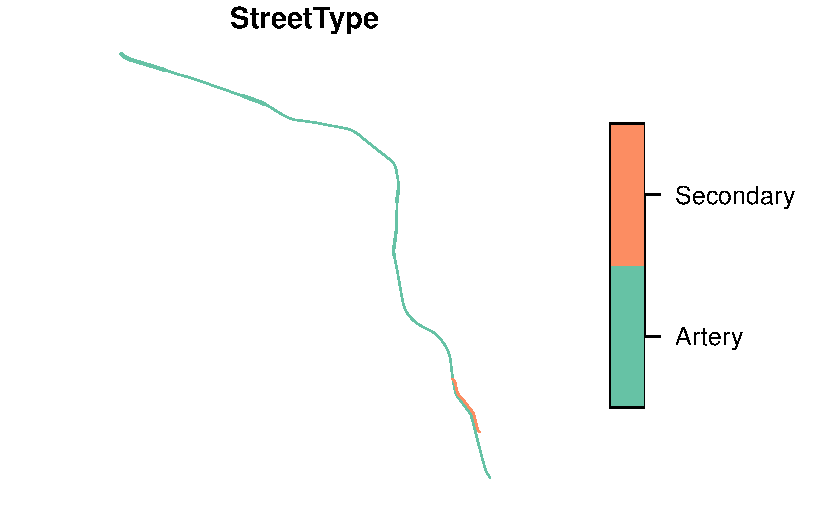
\includegraphics[keepaspectratio]{narrative_vector_files/figure-pdf/unnamed-chunk-9-1.pdf}}

Or using \texttt{ggplot} as:

\begin{Shaded}
\begin{Highlighting}[]
\FunctionTok{ggplot}\NormalTok{( three\_chopt ) }\SpecialCharTok{+} 
  \FunctionTok{geom\_sf}\NormalTok{() }\SpecialCharTok{+} 
  \FunctionTok{coord\_sf}\NormalTok{()}
\end{Highlighting}
\end{Shaded}

\pandocbounded{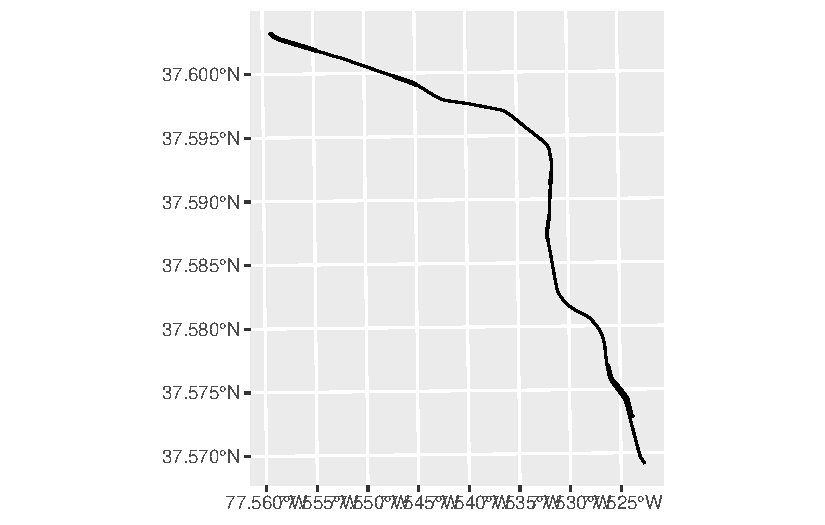
\includegraphics[keepaspectratio]{narrative_vector_files/figure-pdf/unnamed-chunk-10-1.pdf}}

\section{Polygons}\label{polygons}

Polygons are simply lines whose first and last point are the same (e.g.,
they close upon themselves). We can create these \emph{de novo}

\subsection{Polygons from Data Frames}\label{polygons-from-data-frames}

As a first approximation, we can grab polygon data from \texttt{ggplot}
itself. Here I pull in the \texttt{data.frame} representing the counties
of Virginia.

\begin{Shaded}
\begin{Highlighting}[]
\FunctionTok{library}\NormalTok{( maps )}
\end{Highlighting}
\end{Shaded}

\begin{verbatim}

Attaching package: 'maps'
\end{verbatim}

\begin{verbatim}
The following object is masked from 'package:purrr':

    map
\end{verbatim}

\begin{Shaded}
\begin{Highlighting}[]
\FunctionTok{map\_data}\NormalTok{( }\StringTok{"county"}\NormalTok{, }\StringTok{"virginia"}\NormalTok{) }\SpecialCharTok{\%\textgreater{}\%}
  \FunctionTok{select}\NormalTok{( }\AttributeTok{Longitude =}\NormalTok{ long,}
          \AttributeTok{Latitude =}\NormalTok{ lat,}
\NormalTok{          group,}
          \AttributeTok{County =}\NormalTok{ subregion) }\OtherTok{{-}\textgreater{}}\NormalTok{ va\_counties}
\FunctionTok{head}\NormalTok{( va\_counties )}
\end{Highlighting}
\end{Shaded}

\begin{verbatim}
  Longitude Latitude group   County
1 -75.27519 38.03867     1 accomack
2 -75.21790 38.02721     1 accomack
3 -75.21790 38.02721     1 accomack
4 -75.24655 37.99283     1 accomack
5 -75.30384 37.94127     1 accomack
6 -75.31530 37.92981     1 accomack
\end{verbatim}

To get an idea of what theses data represent visually, let's first plot
it as a \texttt{geom\_point()} object. This wil show you where all the
coordinates are located (just not the connecting lines).

\begin{Shaded}
\begin{Highlighting}[]
\FunctionTok{ggplot}\NormalTok{( va\_counties, }\FunctionTok{aes}\NormalTok{( Longitude, Latitude) ) }\SpecialCharTok{+} 
  \FunctionTok{geom\_point}\NormalTok{( }\AttributeTok{size=}\FloatTok{0.25}\NormalTok{ ) }\SpecialCharTok{+} 
  \FunctionTok{coord\_quickmap}\NormalTok{()}
\end{Highlighting}
\end{Shaded}

\pandocbounded{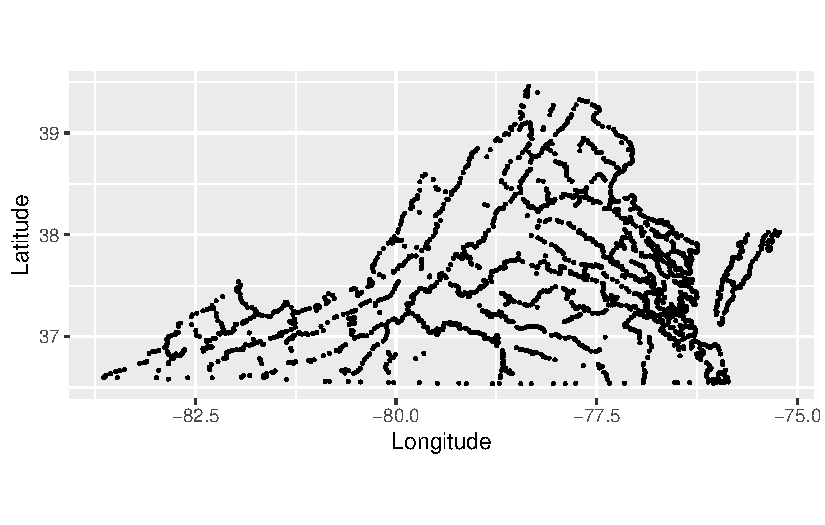
\includegraphics[keepaspectratio]{narrative_vector_files/figure-pdf/unnamed-chunk-12-1.pdf}}

\begin{Shaded}
\begin{Highlighting}[]
\FunctionTok{ggplot}\NormalTok{( va\_counties, }\FunctionTok{aes}\NormalTok{( Longitude, Latitude) ) }\SpecialCharTok{+} 
  \FunctionTok{geom\_polygon}\NormalTok{( }\FunctionTok{aes}\NormalTok{( }\AttributeTok{group=}\NormalTok{group ),}
                \AttributeTok{fill=}\StringTok{"grey80"}\NormalTok{,}
                \AttributeTok{color =} \StringTok{"black"}\NormalTok{, }
                \AttributeTok{size =} \FloatTok{0.25}\NormalTok{) }\SpecialCharTok{+} 
  \FunctionTok{coord\_quickmap}\NormalTok{()}
\end{Highlighting}
\end{Shaded}

\begin{verbatim}
Warning: Using `size` aesthetic for lines was deprecated in ggplot2 3.4.0.
i Please use `linewidth` instead.
\end{verbatim}

\pandocbounded{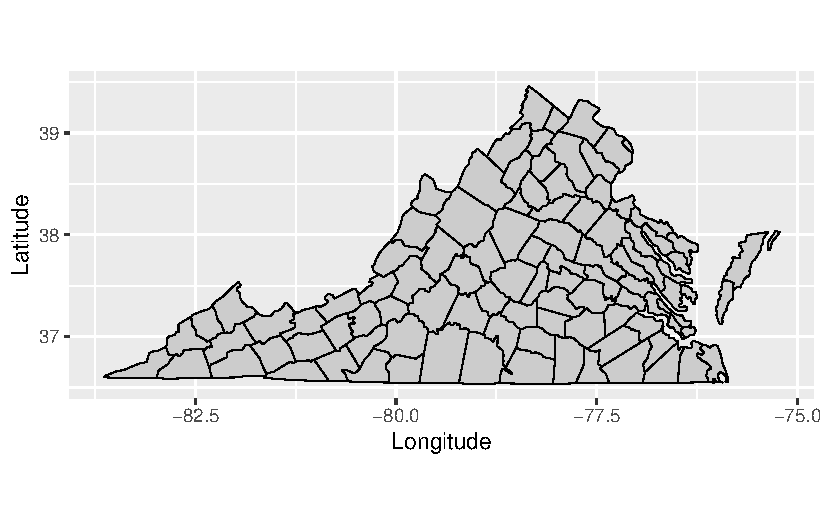
\includegraphics[keepaspectratio]{narrative_vector_files/figure-pdf/unnamed-chunk-13-1.pdf}}

What is hidden here is the complexity of the the points themselves. Each
county is identified by a \texttt{group} in the \texttt{data.frame}

If we look at a particular county, it may be a bit more informative on
how these things are consturcted. Here are the points (in red) and the
underlying connecting lines creating the polygon (in grey).

\begin{Shaded}
\begin{Highlighting}[]
\NormalTok{va\_counties }\SpecialCharTok{\%\textgreater{}\%}
  \FunctionTok{filter}\NormalTok{( County }\SpecialCharTok{\%in\%}  \FunctionTok{c}\NormalTok{(}\StringTok{"hanover"}\NormalTok{,}\StringTok{"henrico"}\NormalTok{) ) }\SpecialCharTok{\%\textgreater{}\%}
  \FunctionTok{ggplot}\NormalTok{( }\FunctionTok{aes}\NormalTok{(Longitude, Latitude) ) }\SpecialCharTok{+} 
  \FunctionTok{geom\_polygon}\NormalTok{( }\FunctionTok{aes}\NormalTok{( }\AttributeTok{fill =}\NormalTok{ County), }\AttributeTok{alpha=}\FloatTok{0.1}\NormalTok{ ) }\SpecialCharTok{+}
  \FunctionTok{geom\_point}\NormalTok{( }\FunctionTok{aes}\NormalTok{( }\AttributeTok{color =}\NormalTok{ County) ) }\SpecialCharTok{+}
  \FunctionTok{coord\_quickmap}\NormalTok{()}
\end{Highlighting}
\end{Shaded}

\pandocbounded{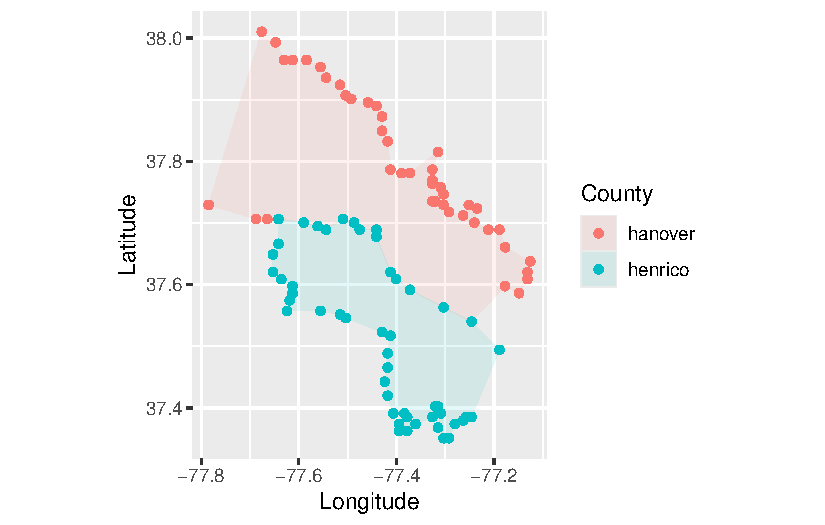
\includegraphics[keepaspectratio]{narrative_vector_files/figure-pdf/unnamed-chunk-14-1.pdf}}

Notice that the points on the border are repeated in both
\texttt{County\ ==\ "hanover"} and \texttt{County\ ==\ "henrico"}.

\subsection{Polygons from Shapefiles}\label{polygons-from-shapefiles}

We can also load these in from shapefiles. In the Richmond GIS data, we
have Zoning District data. We can unzip them in the current directory as
before.

\begin{Shaded}
\begin{Highlighting}[]
\FunctionTok{unzip}\NormalTok{( }\StringTok{"./Districts.zip"}\NormalTok{)}
\end{Highlighting}
\end{Shaded}

And in this case, it simply expands all the files in the current
directory as a set of files named \texttt{Zoning\_Districts.*}.

\begin{Shaded}
\begin{Highlighting}[]
\FunctionTok{system}\NormalTok{(}\StringTok{"ls {-}al Zoning*"}\NormalTok{)}
\end{Highlighting}
\end{Shaded}

To load it in, we read the shapefile (.shp) from the local directory.

\begin{Shaded}
\begin{Highlighting}[]
\NormalTok{districts }\OtherTok{\textless{}{-}} \FunctionTok{st\_read}\NormalTok{( }\StringTok{"Zoning\_Districts.shp"}\NormalTok{ )}
\end{Highlighting}
\end{Shaded}

\begin{verbatim}
Reading layer `Zoning_Districts' from data source 
  `/Users/rodney/Courses/ENVS543-Book/Zoning_Districts.shp' using driver `ESRI Shapefile'
Simple feature collection with 634 features and 14 fields
Geometry type: MULTIPOLYGON
Dimension:     XY
Bounding box:  xmin: 11743500 ymin: 3687944 xmax: 11806060 ymax: 3744741
Projected CRS: NAD83 / Virginia South (ftUS)
\end{verbatim}

\begin{Shaded}
\begin{Highlighting}[]
\FunctionTok{class}\NormalTok{( districts )}
\end{Highlighting}
\end{Shaded}

\begin{verbatim}
[1] "sf"         "data.frame"
\end{verbatim}

This has a lot of columns of information.

\begin{Shaded}
\begin{Highlighting}[]
\FunctionTok{names}\NormalTok{( districts )}
\end{Highlighting}
\end{Shaded}

\begin{verbatim}
 [1] "OBJECTID"   "Name"       "Ordinance"  "OrdinanceP" "Conditiona"
 [6] "AdoptionDa" "Comment"    "CreatedBy"  "CreatedDat" "EditBy"    
[11] "EditDate"   "GlobalID"   "Shape__Are" "Shape__Len" "geometry"  
\end{verbatim}

\begin{Shaded}
\begin{Highlighting}[]
\FunctionTok{summary}\NormalTok{( districts )}
\end{Highlighting}
\end{Shaded}

\begin{verbatim}
    OBJECTID          Name            Ordinance          OrdinanceP       
 Min.   :   1.0   Length:634         Length:634         Length:634        
 1st Qu.: 162.2   Class :character   Class :character   Class :character  
 Median : 324.5   Mode  :character   Mode  :character   Mode  :character  
 Mean   : 389.6                                                           
 3rd Qu.: 486.8                                                           
 Max.   :2677.0                                                           
  Conditiona          AdoptionDa           Comment           CreatedBy        
 Length:634         Min.   :2000-01-01   Length:634         Length:634        
 Class :character   1st Qu.:2000-01-01   Class :character   Class :character  
 Mode  :character   Median :2000-01-01   Mode  :character   Mode  :character  
                    Mean   :2004-01-20                                        
                    3rd Qu.:2007-09-10                                        
                    Max.   :2020-07-27                                        
   CreatedDat            EditBy             EditDate         
 Min.   :2020-08-24   Length:634         Min.   :2020-08-24  
 1st Qu.:2020-08-24   Class :character   1st Qu.:2020-08-24  
 Median :2020-08-24   Mode  :character   Median :2020-08-24  
 Mean   :2020-08-24                      Mean   :2020-08-24  
 3rd Qu.:2020-08-24                      3rd Qu.:2020-08-24  
 Max.   :2020-08-24                      Max.   :2020-08-24  
   GlobalID           Shape__Are          Shape__Len                geometry  
 Length:634         Min.   :     2823   Min.   :   213.4   MULTIPOLYGON :634  
 Class :character   1st Qu.:    71070   1st Qu.:  1232.3   epsg:2284    :  0  
 Mode  :character   Median :   258852   Median :  2552.3   +proj=lcc ...:  0  
                    Mean   :  2749033   Mean   :  6265.9                      
                    3rd Qu.:  1175317   3rd Qu.:  6166.8                      
                    Max.   :171812574   Max.   :111874.1                      
\end{verbatim}

More importantly, we can look at the raw data and see the other meta
data.

\begin{Shaded}
\begin{Highlighting}[]
\FunctionTok{head}\NormalTok{(districts, }\AttributeTok{n=}\DecValTok{2}\NormalTok{)}
\end{Highlighting}
\end{Shaded}

\begin{verbatim}
Simple feature collection with 2 features and 14 fields
Geometry type: MULTIPOLYGON
Dimension:     XY
Bounding box:  xmin: 11773600 ymin: 3730159 xmax: 11789510 ymax: 3731016
Projected CRS: NAD83 / Virginia South (ftUS)
  OBJECTID Name Ordinance OrdinanceP Conditiona AdoptionDa Comment
1        1 RO-2      <NA>       <NA>         No 2000-01-01    <NA>
2        2  B-2      <NA>       <NA>         No 2000-01-01    <NA>
           CreatedBy CreatedDat             EditBy   EditDate
1 richard.morton_cor 2020-08-24 richard.morton_cor 2020-08-24
2 richard.morton_cor 2020-08-24 richard.morton_cor 2020-08-24
                              GlobalID Shape__Are Shape__Len
1 334799f0-fe38-46bf-97c2-260f5a036559   60150.29   983.6815
2 558df9cd-4f9c-4248-a689-bc2d9c79d060   56987.01   971.8832
                        geometry
1 MULTIPOLYGON (((11773598 37...
2 MULTIPOLYGON (((11789222 37...
\end{verbatim}

The whole thing looks like this (I'll use the area of each polygon as
the fill color).

\begin{Shaded}
\begin{Highlighting}[]
\FunctionTok{plot}\NormalTok{( districts[}\StringTok{"Shape\_\_Are"}\NormalTok{], }\AttributeTok{axes=}\ConstantTok{TRUE}\NormalTok{ )}
\end{Highlighting}
\end{Shaded}

\pandocbounded{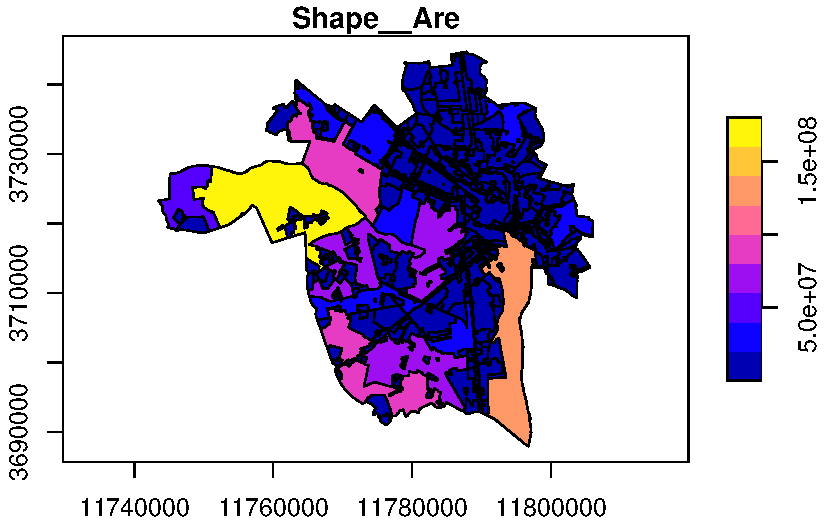
\includegraphics[keepaspectratio]{narrative_vector_files/figure-pdf/unnamed-chunk-21-1.pdf}}

Notice it is in \texttt{CRS\ =\ NAD83/Virginia\ South\ (ftUS)}, which if
we look at \href{http://epsg.io/32147}{epsg.io} and search for it
relates to EPGS=32147. Let's do some pre-processing\footnote{Pielou EC,
  (1984) The interpretation of ecological data: A primer on
  classification and ordination. 288pg. ISBN:
  \href{https://www.wiley.com/en-us/The+Interpretation+of+Ecological+Data\%3A+A+Primer+on+Classification+and+Ordination-p-9780471889502}{978-0-471-88950-2}}:\\
- Put it in Lat/Lon for simplicity\\
- Drop some of the unnecessary columns of data in the shapefile. - Crop
to the VCU/Fan area (I went to google earth and found the bounding box
and then just added it here so I had to make it lat/lon then crop then
change it back).

\begin{Shaded}
\begin{Highlighting}[]
\NormalTok{districts }\SpecialCharTok{\%\textgreater{}\%} 
  \FunctionTok{select}\NormalTok{( OBJECTID, }
\NormalTok{          Name, }
\NormalTok{          GlobalID, }
          \AttributeTok{Area =}\NormalTok{ Shape\_\_Are,}
\NormalTok{          geometry) }\OtherTok{{-}\textgreater{}}\NormalTok{ districts}
\FunctionTok{head}\NormalTok{( districts )}
\end{Highlighting}
\end{Shaded}

\begin{verbatim}
Simple feature collection with 6 features and 4 fields
Geometry type: MULTIPOLYGON
Dimension:     XY
Bounding box:  xmin: 11772310 ymin: 3727332 xmax: 11794670 ymax: 3731016
Projected CRS: NAD83 / Virginia South (ftUS)
  OBJECTID Name                             GlobalID      Area
1        1 RO-2 334799f0-fe38-46bf-97c2-260f5a036559  60150.29
2        2  B-2 558df9cd-4f9c-4248-a689-bc2d9c79d060  56987.01
3        3  R-6 8d731cd3-7cfb-41d4-9545-44f1055515b3  93826.03
4        4  B-1 f4fb1283-03ff-41e7-b5ed-3cf6e80c2e9b  17526.31
5        5  B-1 f1305477-4e71-463c-a202-332971d8c5e1  33261.30
6        6 RO-1 65e43734-9728-4241-921d-c657137dae0a 132773.19
                        geometry
1 MULTIPOLYGON (((11773598 37...
2 MULTIPOLYGON (((11789222 37...
3 MULTIPOLYGON (((11774598 37...
4 MULTIPOLYGON (((11794468 37...
5 MULTIPOLYGON (((11781126 37...
6 MULTIPOLYGON (((11772306 37...
\end{verbatim}

And we can plot it normally using \texttt{plot()} for \texttt{sf}
objects. Each row is a \texttt{MULTIPOLYGON} object.

\begin{Shaded}
\begin{Highlighting}[]
\NormalTok{districts }\SpecialCharTok{\%\textgreater{}\%}
  \FunctionTok{filter}\NormalTok{( OBJECTID }\SpecialCharTok{==} \DecValTok{368}\NormalTok{ ) }\SpecialCharTok{\%\textgreater{}\%}
  \FunctionTok{st\_buffer}\NormalTok{(}\AttributeTok{dist =} \DecValTok{1500}\NormalTok{) }\SpecialCharTok{\%\textgreater{}\%}
  \FunctionTok{st\_bbox}\NormalTok{() }\OtherTok{{-}\textgreater{}}\NormalTok{ fan\_bbox}
\NormalTok{districts }\SpecialCharTok{\%\textgreater{}\%}
  \FunctionTok{st\_crop}\NormalTok{( fan\_bbox ) }\OtherTok{{-}\textgreater{}}\NormalTok{ theFan }
\end{Highlighting}
\end{Shaded}

\begin{verbatim}
Warning: attribute variables are assumed to be spatially constant throughout
all geometries
\end{verbatim}

\begin{Shaded}
\begin{Highlighting}[]
\FunctionTok{plot}\NormalTok{( theFan[}\StringTok{"Name"}\NormalTok{] )}
\end{Highlighting}
\end{Shaded}

\pandocbounded{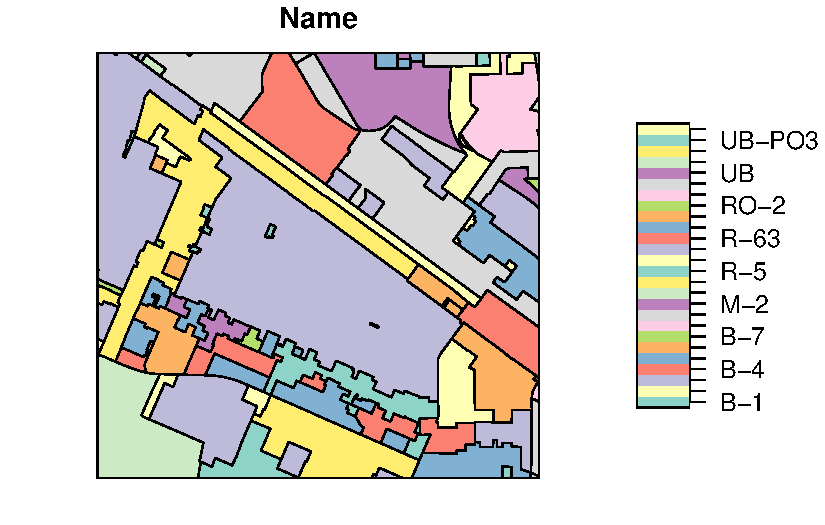
\includegraphics[keepaspectratio]{narrative_vector_files/figure-pdf/unnamed-chunk-23-1.pdf}}

Or as a \texttt{ggplot()} object (notice how it converts to lat/lon when
plotting),

\begin{Shaded}
\begin{Highlighting}[]
\FunctionTok{ggplot}\NormalTok{( theFan ) }\SpecialCharTok{+} 
  \FunctionTok{geom\_sf}\NormalTok{( }\FunctionTok{aes}\NormalTok{( }\AttributeTok{fill=}\NormalTok{Name ) ) }\SpecialCharTok{+} 
  \FunctionTok{coord\_sf}\NormalTok{() }
\end{Highlighting}
\end{Shaded}

\pandocbounded{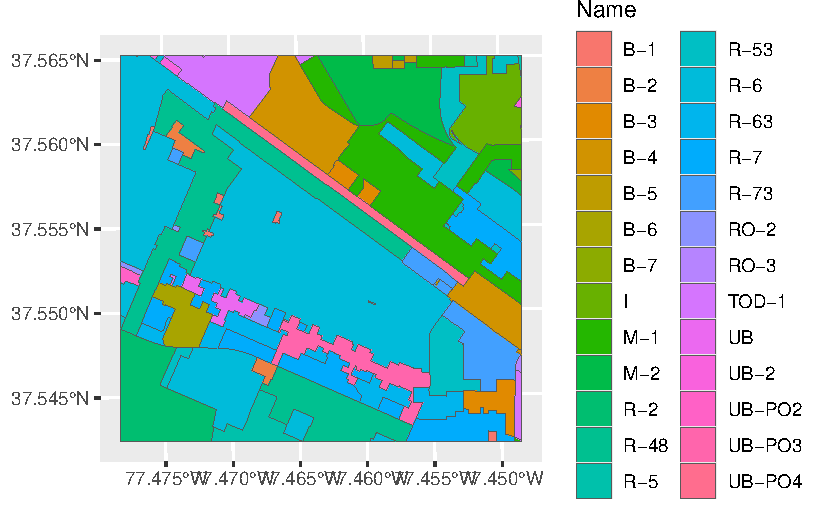
\includegraphics[keepaspectratio]{narrative_vector_files/figure-pdf/unnamed-chunk-24-1.pdf}}

Let's go grab a key to those zoning types. I've uploaded a csv file with
a translation. Here I \texttt{left\_join()} with that new file that is
read in dynamically\footnote{You should be careful when you use joins on
  \texttt{sf} objects. If you \texttt{sf} object is on the right side
  (see discussion of joins
  \href{https://dyerlab.github.io/ENVS-Lectures/manipulation/relational_data/slides.html\#5}{here})
  then the result will not be an \texttt{sf} object and you'll have to
  coerce it back into one again. It always adopts the characteristics of
  the left object.}.

\begin{Shaded}
\begin{Highlighting}[]
\NormalTok{zone\_url }\OtherTok{\textless{}{-}} \StringTok{"https://raw.githubusercontent.com/dyerlab/ENVS{-}Lectures/master/data/DistrictCodes.csv"}
\NormalTok{theFan }\SpecialCharTok{\%\textgreater{}\%}
  \FunctionTok{left\_join}\NormalTok{( }\FunctionTok{read\_csv}\NormalTok{( zone\_url ),}
             \AttributeTok{by=}\StringTok{"Name"}\NormalTok{) }\SpecialCharTok{\%\textgreater{}\%}
  \FunctionTok{mutate}\NormalTok{( }\AttributeTok{Category =} \FunctionTok{factor}\NormalTok{( Category) ) }\SpecialCharTok{\%\textgreater{}\%}
  \FunctionTok{select}\NormalTok{( OBJECTID, }
\NormalTok{          Name, }
\NormalTok{          Category, }
          \FunctionTok{everything}\NormalTok{() )  }\OtherTok{{-}\textgreater{}}\NormalTok{ theFan}
\end{Highlighting}
\end{Shaded}

\begin{verbatim}
Rows: 27 Columns: 2
-- Column specification --------------------------------------------------------
Delimiter: ","
chr (2): Name, Category

i Use `spec()` to retrieve the full column specification for this data.
i Specify the column types or set `show_col_types = FALSE` to quiet this message.
\end{verbatim}

\begin{Shaded}
\begin{Highlighting}[]
\FunctionTok{ggplot}\NormalTok{( theFan ) }\SpecialCharTok{+}
  \FunctionTok{geom\_sf}\NormalTok{( }\FunctionTok{aes}\NormalTok{( }\AttributeTok{fill=}\NormalTok{Category)) }\SpecialCharTok{+}
  \FunctionTok{scale\_fill\_brewer}\NormalTok{( }\AttributeTok{type=}\StringTok{"qual"}\NormalTok{, }
                     \AttributeTok{palette =} \StringTok{"Set3"}\NormalTok{)}
\end{Highlighting}
\end{Shaded}

\pandocbounded{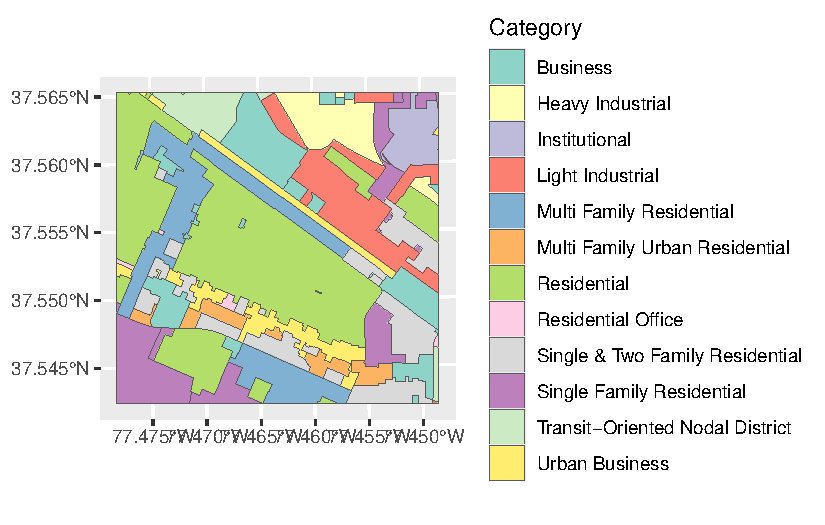
\includegraphics[keepaspectratio]{narrative_vector_files/figure-pdf/unnamed-chunk-26-1.pdf}}

\section{Operations}\label{operations}

So we will close this out by looking at a few different operations that
we can use for polygons. First, I'm going to load in the road shapefile
(that was named by some random sequence of letters) and reproject it.

\begin{Shaded}
\begin{Highlighting}[]
\FunctionTok{head}\NormalTok{( roads, }\AttributeTok{n=}\DecValTok{3}\NormalTok{)}
\end{Highlighting}
\end{Shaded}

\begin{verbatim}
Simple feature collection with 3 features and 6 fields
Geometry type: LINESTRING
Dimension:     XY
Bounding box:  xmin: 11775970 ymin: 3733301 xmax: 11786050 ymax: 3740059
Projected CRS: NAD83 / Virginia South (ftUS)
  FIPS AssetID StreetType Functional    FullName OneWay
1  760       2  Secondary      Local   Sauer Ave   <NA>
2  760       3  Secondary      Local   Sauer Ave   <NA>
3  760      89  Secondary      Local Amherst Ave   <NA>
                        geometry
1 LINESTRING (11775968 373330...
2 LINESTRING (11775997 373334...
3 LINESTRING (11785407 374003...
\end{verbatim}

\begin{Shaded}
\begin{Highlighting}[]
\FunctionTok{plot}\NormalTok{( theFan}\SpecialCharTok{$}\NormalTok{geometry, }\AttributeTok{lwd=}\DecValTok{2}\NormalTok{ )}
\NormalTok{fanRoads }\OtherTok{\textless{}{-}} \FunctionTok{st\_crop}\NormalTok{( roads, }\FunctionTok{st\_bbox}\NormalTok{( theFan ))}
\end{Highlighting}
\end{Shaded}

\begin{verbatim}
Warning: attribute variables are assumed to be spatially constant throughout
all geometries
\end{verbatim}

\begin{Shaded}
\begin{Highlighting}[]
\FunctionTok{plot}\NormalTok{( fanRoads}\SpecialCharTok{$}\NormalTok{geometry, }\AttributeTok{col=}\StringTok{"blue"}\NormalTok{, }\AttributeTok{cex=}\FloatTok{0.5}\NormalTok{, }\AttributeTok{add=}\ConstantTok{TRUE}\NormalTok{ )}
\end{Highlighting}
\end{Shaded}

\pandocbounded{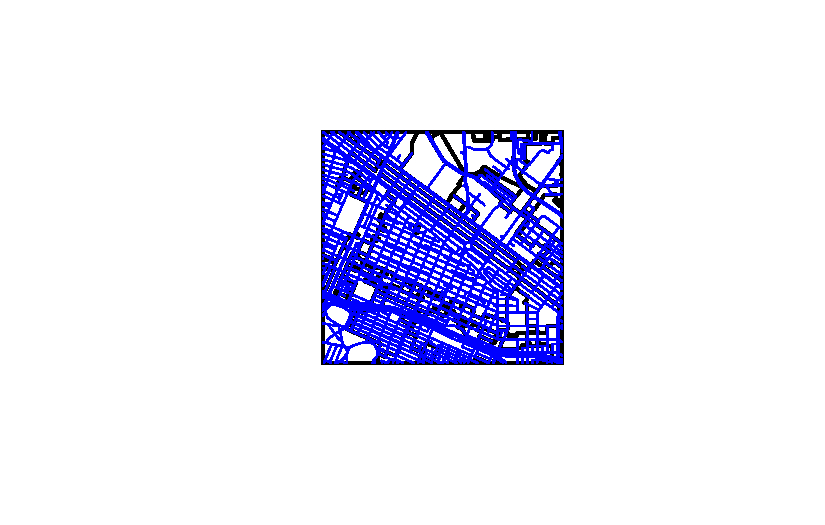
\includegraphics[keepaspectratio]{narrative_vector_files/figure-pdf/unnamed-chunk-28-1.pdf}}

Let's isolate one of the main polygons in \texttt{theFan} data set. The
target one below is indicated by \texttt{OBJECTID=368}.

\begin{Shaded}
\begin{Highlighting}[]
\NormalTok{theFan }\SpecialCharTok{\%\textgreater{}\%}
  \FunctionTok{mutate}\NormalTok{( }\AttributeTok{Target =} \FunctionTok{ifelse}\NormalTok{( OBJECTID }\SpecialCharTok{==} \DecValTok{368}\NormalTok{, }
                           \ConstantTok{TRUE}\NormalTok{, }
                           \ConstantTok{FALSE}\NormalTok{) ) }\OtherTok{{-}\textgreater{}}\NormalTok{ theFan}
\NormalTok{theFan }\SpecialCharTok{\%\textgreater{}\%}
  \FunctionTok{ggplot}\NormalTok{() }\SpecialCharTok{+} 
  \FunctionTok{geom\_sf}\NormalTok{( }\FunctionTok{aes}\NormalTok{(}\AttributeTok{fill=}\NormalTok{Target) ) }\SpecialCharTok{+} 
  \FunctionTok{geom\_sf\_text}\NormalTok{( }\FunctionTok{aes}\NormalTok{(}\AttributeTok{label=}\NormalTok{OBJECTID), }\AttributeTok{size=}\DecValTok{3}\NormalTok{ ) }\SpecialCharTok{+}
  \FunctionTok{coord\_sf}\NormalTok{() }
\end{Highlighting}
\end{Shaded}

\pandocbounded{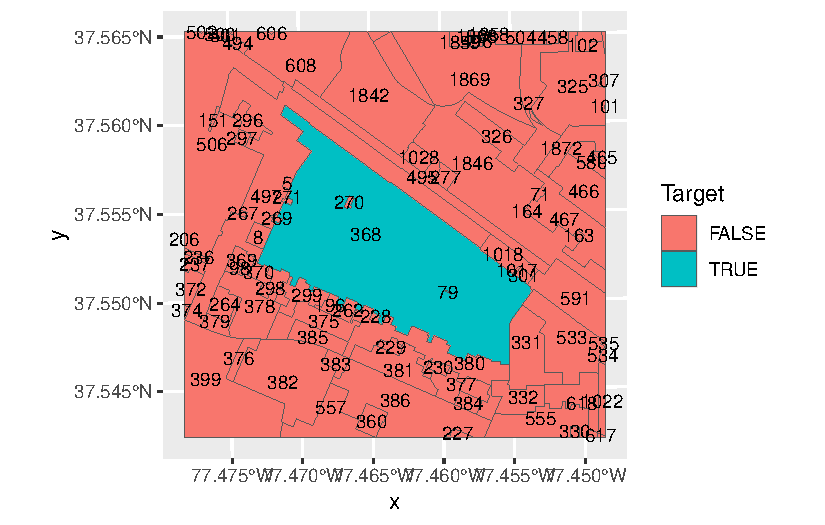
\includegraphics[keepaspectratio]{narrative_vector_files/figure-pdf/unnamed-chunk-29-1.pdf}}

\section{Spatial Joins}\label{spatial-joins}

\begin{Shaded}
\begin{Highlighting}[]
\FunctionTok{names}\NormalTok{( theFan )}
\end{Highlighting}
\end{Shaded}

\begin{verbatim}
[1] "OBJECTID" "Name"     "Category" "GlobalID" "Area"     "geometry" "Target"  
\end{verbatim}

\begin{Shaded}
\begin{Highlighting}[]
\FunctionTok{names}\NormalTok{( fanRoads )}
\end{Highlighting}
\end{Shaded}

\begin{verbatim}
[1] "FIPS"       "AssetID"    "StreetType" "Functional" "FullName"  
[6] "OneWay"     "geometry"  
\end{verbatim}

We can use \emph{spatial joins} to select features either directly. Here
I'll use the target polygon in \texttt{theFan}

\begin{Shaded}
\begin{Highlighting}[]
\NormalTok{target }\OtherTok{\textless{}{-}}\NormalTok{ theFan[ theFan}\SpecialCharTok{$}\NormalTok{OBJECTID }\SpecialCharTok{==} \DecValTok{368}\NormalTok{, ]}
\NormalTok{target}
\end{Highlighting}
\end{Shaded}

\begin{verbatim}
Simple feature collection with 1 feature and 6 fields
Geometry type: POLYGON
Dimension:     XY
Bounding box:  xmin: 11780610 ymin: 3724146 xmax: 11786260 ymax: 3729483
Projected CRS: NAD83 / Virginia South (ftUS)
   OBJECTID Name    Category                             GlobalID     Area
39      368  R-6 Residential d9882dad-2625-44e7-a170-3f1425450679 13040977
                         geometry Target
39 POLYGON ((11785188 3726513,...   TRUE
\end{verbatim}

And then add an attribute to the \texttt{data.frame} if each
multipolygon \texttt{intersects} that polygon.

\begin{Shaded}
\begin{Highlighting}[]
\NormalTok{fanRoads }\SpecialCharTok{\%\textgreater{}\%}
  \FunctionTok{mutate}\NormalTok{( }\AttributeTok{OnTarget =} \FunctionTok{st\_intersects}\NormalTok{( fanRoads,}
\NormalTok{                                    target, }
                                    \AttributeTok{sparse =} \ConstantTok{FALSE}\NormalTok{ ) ) }\OtherTok{{-}\textgreater{}}\NormalTok{ fanRoads}
\FunctionTok{summary}\NormalTok{( fanRoads}\SpecialCharTok{$}\NormalTok{OnTarget )}
\end{Highlighting}
\end{Shaded}

\begin{verbatim}
     V1         
 Mode :logical  
 FALSE:1567     
 TRUE :553      
\end{verbatim}

We can get the names of these road using normal \texttt{dplyr} routines,

\begin{Shaded}
\begin{Highlighting}[]
\NormalTok{fanRoads }\SpecialCharTok{\%\textgreater{}\%}
  \FunctionTok{filter}\NormalTok{( }\FunctionTok{st\_intersects}\NormalTok{( fanRoads,}
\NormalTok{                         target, }
                         \AttributeTok{sparse =} \ConstantTok{FALSE}\NormalTok{ ) }\SpecialCharTok{==} \ConstantTok{TRUE}\NormalTok{ ) }\SpecialCharTok{\%\textgreater{}\%}
  \FunctionTok{as\_data\_frame}\NormalTok{() }\SpecialCharTok{\%\textgreater{}\%}
  \FunctionTok{select}\NormalTok{( }\StringTok{\textasciigrave{}}\AttributeTok{Street Name}\StringTok{\textasciigrave{}} \OtherTok{=}\NormalTok{ FullName ) }\SpecialCharTok{\%\textgreater{}\%}
  \FunctionTok{arrange}\NormalTok{( }\StringTok{\textasciigrave{}}\AttributeTok{Street Name}\StringTok{\textasciigrave{}}\NormalTok{) }\SpecialCharTok{\%\textgreater{}\%}
  \FunctionTok{unique}\NormalTok{() }
\end{Highlighting}
\end{Shaded}

\begin{verbatim}
Warning: `as_data_frame()` was deprecated in tibble 2.0.0.
i Please use `as_tibble()` (with slightly different semantics) to convert to a
  tibble, or `as.data.frame()` to convert to a data frame.
\end{verbatim}

\begin{verbatim}
Warning: Using one column matrices in `filter()` or `filter_out()` was deprecated in
dplyr 1.1.0.
i Please use one dimensional logical vectors instead.
\end{verbatim}

\begin{verbatim}
# A tibble: 39 x 1
   `Street Name` 
   <chr>         
 1 Allison St    
 2 Birch St      
 3 Boyd St       
 4 Floyd Ave     
 5 Grove Ave     
 6 Hanover Ave   
 7 Kensington Ave
 8 Lombardy Pl   
 9 Madumbie Lane 
10 Monument Ave  
# i 29 more rows
\end{verbatim}

And we can plot them as:

\begin{Shaded}
\begin{Highlighting}[]
\NormalTok{fanRoads }\SpecialCharTok{\%\textgreater{}\%}
  \FunctionTok{filter}\NormalTok{( OnTarget}\SpecialCharTok{==}\ConstantTok{TRUE}\NormalTok{ ) }\SpecialCharTok{\%\textgreater{}\%}
  \FunctionTok{ggplot}\NormalTok{() }\SpecialCharTok{+}
  \FunctionTok{geom\_sf}\NormalTok{( }\FunctionTok{aes}\NormalTok{( }\AttributeTok{fill =}\NormalTok{ Target ), }\AttributeTok{data=}\NormalTok{theFan ) }\SpecialCharTok{+}
  \FunctionTok{geom\_sf}\NormalTok{( }\AttributeTok{color=}\StringTok{"green"}\NormalTok{ ) }\SpecialCharTok{+} 
  \FunctionTok{scale\_fill\_manual}\NormalTok{( }\AttributeTok{values=}\FunctionTok{c}\NormalTok{(}\StringTok{"grey90"}\NormalTok{,}\StringTok{"dodgerblue3"}\NormalTok{))}
\end{Highlighting}
\end{Shaded}

\begin{verbatim}
Warning: Using one column matrices in `filter()` or `filter_out()` was deprecated in
dplyr 1.1.0.
i Please use one dimensional logical vectors instead.
\end{verbatim}

\pandocbounded{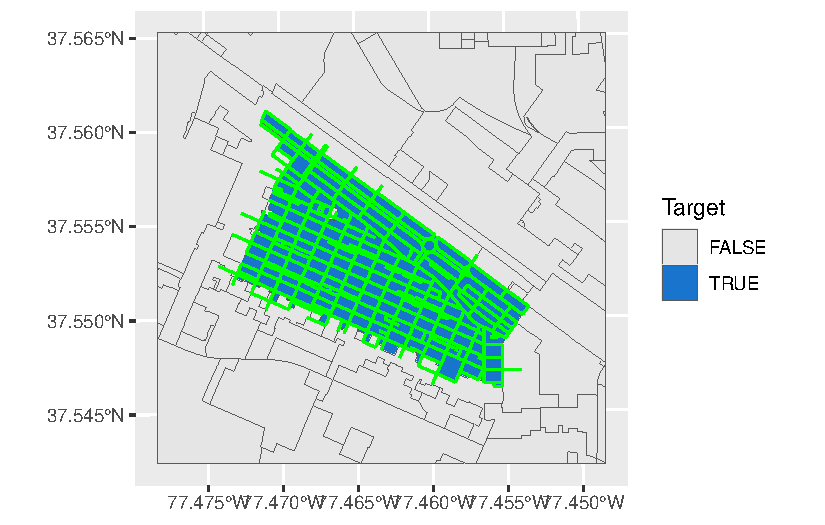
\includegraphics[keepaspectratio]{narrative_vector_files/figure-pdf/unnamed-chunk-34-1.pdf}}

Go check out the \texttt{sf} cheatsheet for more geospatial joins and
options.

\chapter{Raster Data}\label{raster-data}

\pandocbounded{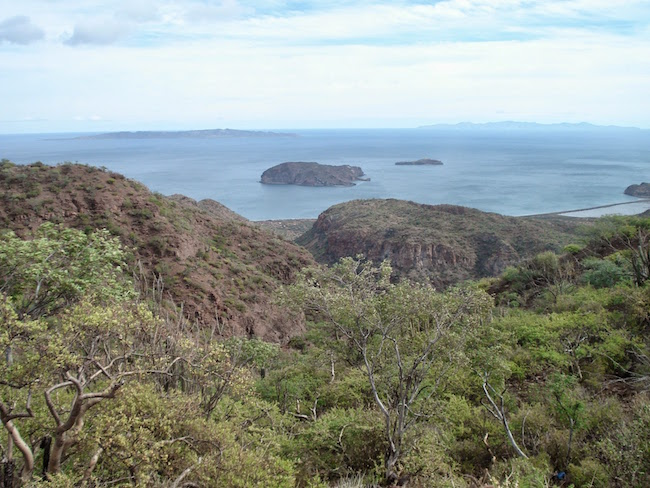
\includegraphics[keepaspectratio]{media/chapter_raster.jpg}}

\begin{quote}
Raster data is good for representing continuous surfaces and performing
fast analyses on large areas, such as calculating a surface temperature
map or a land-cover classification.
\end{quote}

\section{Lecture Materials}\label{lecture-materials-10}

\begin{quote}
\textbf{Lecture Slides:} Available interactively in the
\href{https://dyerlabteaching.github.io/Raster-Data/slides.html\#/title-slide}{online
version}
\end{quote}

\begin{figure}[H]

{\centering \pandocbounded{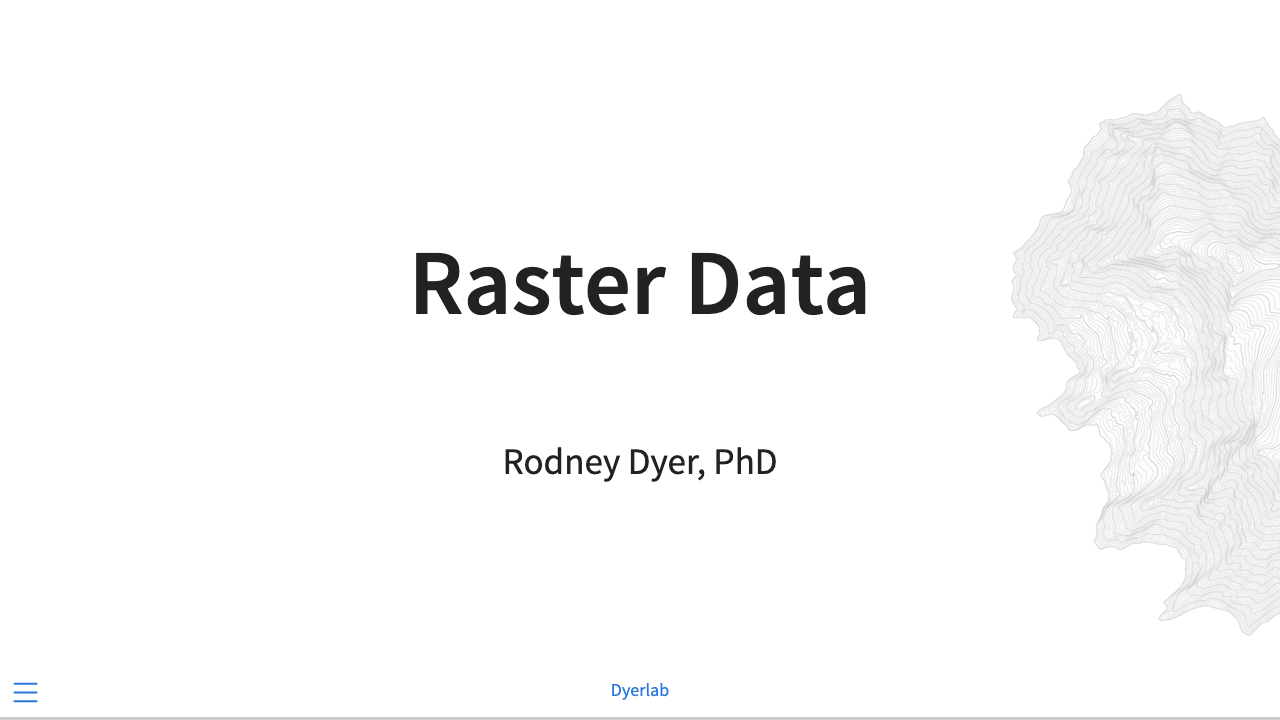
\includegraphics[keepaspectratio]{media/slides_rasters.png}}

}

\caption{Lecture Slides}

\end{figure}%

All raster operations in this topic are accomplished using the
\texttt{raster} library.

\begin{Shaded}
\begin{Highlighting}[]
\FunctionTok{library}\NormalTok{(raster)}
\end{Highlighting}
\end{Shaded}

\begin{verbatim}
Loading required package: sp
\end{verbatim}

Raster are representations of continuous, or semi-continuous, data. TYou
can envision a raster just like an image. When me make a
\texttt{leaflet()} map and how the tiles, each pixel is colored a
particular value representing elevation, temperature, precipitation,
habitat type, or whatever. This is exactly the same for rasters. The
\emph{key point} here is that each pixel represents some defined region
on the earth and as such the raster itself is georeferenced. It has a
coordinate reference system (CRS), boundaries, etc.

\section{\texorpdfstring{Making Rasters \emph{de
novo}}{Making Rasters de novo}}\label{making-rasters-de-novo}

A raster is simply a matrix with rows and columns and each element has a
value associated with it. You can create a raster \emph{de novo} by
making a matrix of data and filling it with values, then turning it into
a raster.

Here I make a raster with random numbrers selected from the Poisson
Distribution (fishy, I know) using the \texttt{rpois()} function. I then
turn it into a matrix with 7 rows (and 7 columns).

\begin{Shaded}
\begin{Highlighting}[]
\NormalTok{vals }\OtherTok{\textless{}{-}} \FunctionTok{rpois}\NormalTok{(}\DecValTok{49}\NormalTok{, }\AttributeTok{lambda=}\DecValTok{12}\NormalTok{)}
\NormalTok{x }\OtherTok{\textless{}{-}} \FunctionTok{matrix}\NormalTok{( vals, }\AttributeTok{nrow=}\DecValTok{7}\NormalTok{)}
\NormalTok{x}
\end{Highlighting}
\end{Shaded}

\begin{verbatim}
     [,1] [,2] [,3] [,4] [,5] [,6] [,7]
[1,]   14   14   10   14   10   15   13
[2,]    4   10   11    8   13   10    8
[3,]    9   11    9   20    9   10   12
[4,]   10   12   13   13   13   15   14
[5,]    9   18    6   16   14   14   17
[6,]   12   11    6   12    9   10    8
[7,]   12    6   14   10    6    3   11
\end{verbatim}

While we haven't used matrices much thus far, it is a lot like a
\texttt{data.frame} with respect to getting and setting values using
numerical indices. For example, the value of the 3rd row and 5th column
is:

\begin{Shaded}
\begin{Highlighting}[]
\NormalTok{x[}\DecValTok{3}\NormalTok{,}\DecValTok{5}\NormalTok{]}
\end{Highlighting}
\end{Shaded}

\begin{verbatim}
[1] 9
\end{verbatim}

To convert this set of data, as a matrix, into a geospatially referenced
\texttt{raster()} object we do the following:

\begin{Shaded}
\begin{Highlighting}[]
\NormalTok{r }\OtherTok{\textless{}{-}} \FunctionTok{raster}\NormalTok{( x )}
\NormalTok{r}
\end{Highlighting}
\end{Shaded}

\begin{verbatim}
class      : RasterLayer 
dimensions : 7, 7, 49  (nrow, ncol, ncell)
resolution : 0.1428571, 0.1428571  (x, y)
extent     : 0, 1, 0, 1  (xmin, xmax, ymin, ymax)
crs        : NA 
source     : memory
names      : layer 
values     : 3, 20  (min, max)
\end{verbatim}

Notice that when I plot it out, it does not show the data, but a summary
of the data along with some key data about the contents, including:\\
- A class definition\\
- The dimensions of the underlying data matrix,\\
- The resolution (e.g., the spatial extent of the sides of each pixel).
Since we have no CRS here, it is equal to \(nrows(x)^{-1}\) and
\(ncols(x)^{-1}\).\\
- The extent (the bounding box) and again since we do not have a CRS
defined it just goes from \(0\) to \(1\). - The \texttt{crs} (missing) -
The source can be either \texttt{memory} if the raster is not that big
or \texttt{out\ of\ memory} if it is just referencing.

If these data represent something on the planet, we can assign the
dimensions and \texttt{CRS} values to it and use it in our normal
day-to-day operations.

\section{Loading Rasters from Files or
URLs}\label{loading-rasters-from-files-or-urls}

We can also grab a raster object from the filesystem or from some online
repository by passing the link to the \texttt{raster()} function. Here
is the elevation, in meters, of the region in which Mexico is found. To
load it in, pass the url.

\begin{Shaded}
\begin{Highlighting}[]
\NormalTok{url }\OtherTok{\textless{}{-}} \StringTok{"https://github.com/DyerlabTeaching/Raster{-}Data/raw/main/data/alt\_22.tif"}
\NormalTok{r }\OtherTok{\textless{}{-}} \FunctionTok{raster}\NormalTok{( url )}
\NormalTok{r}
\end{Highlighting}
\end{Shaded}

\begin{verbatim}
class      : RasterLayer 
dimensions : 3600, 3600, 12960000  (nrow, ncol, ncell)
resolution : 0.008333333, 0.008333333  (x, y)
extent     : -120, -90, 4.163336e-16, 30  (xmin, xmax, ymin, ymax)
crs        : +proj=longlat +datum=WGS84 +no_defs 
source     : alt_22.tif 
names      : alt_22 
values     : -202, 5469  (min, max)
\end{verbatim}

Notice that this raster has a defined CRS and as such it is projected
and the extent relates to the units of the datum (e.g., from -120 to -90
degrees longitude and 0 to 30 degrees latitude).

If we plot it, we can see the whole raster.

\begin{Shaded}
\begin{Highlighting}[]
\FunctionTok{plot}\NormalTok{(r)}
\end{Highlighting}
\end{Shaded}

\pandocbounded{
\includegraphics[keepaspectratio]{narrative_rasters_files/figure-pdf/unnamed-chunk-6-1.pdf}}

Now, this raster is elevation where there is land but where there is no
land, it is full of \texttt{NA} values. As such, there is a ton of them.

\begin{Shaded}
\begin{Highlighting}[]
\FunctionTok{format}\NormalTok{( }\FunctionTok{sum}\NormalTok{( }\FunctionTok{is.na}\NormalTok{( }\FunctionTok{values}\NormalTok{(r) ) ), }\AttributeTok{big.mark =} \StringTok{","}\NormalTok{ )}
\end{Highlighting}
\end{Shaded}

\begin{verbatim}
[1] "10,490,650"
\end{verbatim}

\section{Cropping}\label{cropping}

One of the first things to do is to crop the data down to represent the
size and extent of our study area. If we over 10 million missing data
points (the ocean) and most of Mexico in this raster above but we are
only working with sites in Baja California (Norte y Sur), we would do
well to excise (or crop) the raster to only include the area we are
interested in working with.

Top do this, we need to figure out a bounding box (e.g., the minimim and
maximum values of longitude and latitude that enclose our data). Let's
assume we are working with the Beetle Data from the
\href{https://dyerlab.github.io/ENVS-Lectures/spatial/spatial_points/slides.html\#1}{Spatial
Points Slides} and load in the Sex-biased dispersal data set and use
those points as a starting estimate of the bounding box.

\begin{Shaded}
\begin{Highlighting}[]
\FunctionTok{library}\NormalTok{( sf )}
\end{Highlighting}
\end{Shaded}

\begin{verbatim}
Linking to GEOS 3.13.0, GDAL 3.8.5, PROJ 9.5.1; sf_use_s2() is TRUE
\end{verbatim}

\begin{Shaded}
\begin{Highlighting}[]
\FunctionTok{library}\NormalTok{( tidyverse )}
\end{Highlighting}
\end{Shaded}

\begin{verbatim}
-- Attaching core tidyverse packages ------------------------ tidyverse 2.0.0 --
v dplyr     1.2.1     v readr     2.2.0
v forcats   1.0.1     v stringr   1.6.0
v ggplot2   4.0.2     v tibble    3.3.1
v lubridate 1.9.5     v tidyr     1.3.2
v purrr     1.2.1     
\end{verbatim}

\begin{verbatim}
-- Conflicts ------------------------------------------ tidyverse_conflicts() --
x tidyr::extract() masks raster::extract()
x dplyr::filter()  masks stats::filter()
x dplyr::lag()     masks stats::lag()
x dplyr::select()  masks raster::select()
i Use the conflicted package (<http://conflicted.r-lib.org/>) to force all conflicts to become errors
\end{verbatim}

\begin{Shaded}
\begin{Highlighting}[]
\NormalTok{beetle\_url }\OtherTok{\textless{}{-}} \StringTok{"https://raw.githubusercontent.com/dyerlab/ENVS{-}Lectures/master/data/Araptus\_Disperal\_Bias.csv"}

\FunctionTok{read\_csv}\NormalTok{( beetle\_url ) }\SpecialCharTok{\%\textgreater{}\%}
  \FunctionTok{st\_as\_sf}\NormalTok{( }\AttributeTok{coords=}\FunctionTok{c}\NormalTok{(}\StringTok{"Longitude"}\NormalTok{,}\StringTok{"Latitude"}\NormalTok{), }\AttributeTok{crs=}\DecValTok{4326}\NormalTok{ ) }\OtherTok{{-}\textgreater{}}\NormalTok{ beetles}
\end{Highlighting}
\end{Shaded}

\begin{verbatim}
Rows: 31 Columns: 9
-- Column specification --------------------------------------------------------
Delimiter: ","
chr (1): Site
dbl (8): Males, Females, Suitability, MFRatio, GenVarArapat, GenVarEuphli, L...

i Use `spec()` to retrieve the full column specification for this data.
i Specify the column types or set `show_col_types = FALSE` to quiet this message.
\end{verbatim}

\begin{Shaded}
\begin{Highlighting}[]
\FunctionTok{summary}\NormalTok{( beetles )}
\end{Highlighting}
\end{Shaded}

\begin{verbatim}
     Site               Males          Females       Suitability    
 Length:31          Min.   : 9.00   Min.   : 5.00   Min.   :0.0563  
 Class :character   1st Qu.:16.00   1st Qu.:15.50   1st Qu.:0.2732  
 Mode  :character   Median :21.00   Median :21.00   Median :0.3975  
                    Mean   :25.68   Mean   :23.52   Mean   :0.4276  
                    3rd Qu.:31.50   3rd Qu.:29.00   3rd Qu.:0.5442  
                    Max.   :64.00   Max.   :63.00   Max.   :0.9019  
    MFRatio        GenVarArapat     GenVarEuphli             geometry 
 Min.   :0.5938   Min.   :0.0500   Min.   :0.0500   POINT        :31  
 1st Qu.:0.8778   1st Qu.:0.1392   1st Qu.:0.1777   epsg:4326    : 0  
 Median :1.1200   Median :0.2002   Median :0.2171   +proj=long...: 0  
 Mean   :1.1598   Mean   :0.2006   Mean   :0.2203                     
 3rd Qu.:1.3618   3rd Qu.:0.2592   3rd Qu.:0.2517                     
 Max.   :2.2000   Max.   :0.3379   Max.   :0.5122                     
\end{verbatim}

Now, we can take the bounding box of these points and get a first
approximation.

\begin{Shaded}
\begin{Highlighting}[]
\NormalTok{beetles }\SpecialCharTok{\%\textgreater{}\%} \FunctionTok{st\_bbox}\NormalTok{()}
\end{Highlighting}
\end{Shaded}

\begin{verbatim}
      xmin       ymin       xmax       ymax 
-114.29353   23.28550 -109.32700   29.32541 
\end{verbatim}

OK, so this is the strict bounding box for these points. This means that
the minimum and maximum values for these points are defined by the
original locations---for both the latitude and longitude (both minimum
and maximum)---we have sites on each of the edges. This is fine here but
we could probably add a little bit of a \emph{buffer} around that
bounding box so that we do not have our sites on the very edge of the
plot. We can do this by either \emph{eyeballing-it} to round up to some
reasonable area around the points \emph{or} apply a buffer
(\texttt{st\_buffer}) to the union of all the points with some distance
and then take the boounding box. I'll go for the former and make it into
an \texttt{extent} object.

\begin{Shaded}
\begin{Highlighting}[]
\NormalTok{baja\_extent }\OtherTok{\textless{}{-}} \FunctionTok{extent}\NormalTok{( }\FunctionTok{c}\NormalTok{(}\SpecialCharTok{{-}}\DecValTok{116}\NormalTok{, }\SpecialCharTok{{-}}\DecValTok{109}\NormalTok{, }\DecValTok{22}\NormalTok{, }\DecValTok{30}\NormalTok{ ) )}
\NormalTok{baja\_extent}
\end{Highlighting}
\end{Shaded}

\begin{verbatim}
class      : Extent 
xmin       : -116 
xmax       : -109 
ymin       : 22 
ymax       : 30 
\end{verbatim}

Then we can \texttt{crop()} the original raster using this extent object
to create our working raster. I can then dump my points onto the same
raster plot by indicaating \texttt{add=TRUE}

\begin{Shaded}
\begin{Highlighting}[]
\NormalTok{alt }\OtherTok{\textless{}{-}} \FunctionTok{crop}\NormalTok{( r, baja\_extent )}
\FunctionTok{plot}\NormalTok{(alt)}
\FunctionTok{plot}\NormalTok{( beetles[}\StringTok{"Suitability"}\NormalTok{], }\AttributeTok{pch=}\DecValTok{16}\NormalTok{, }\AttributeTok{add=}\ConstantTok{TRUE}\NormalTok{)}
\end{Highlighting}
\end{Shaded}

\pandocbounded{
\includegraphics[keepaspectratio]{narrative_rasters_files/figure-pdf/unnamed-chunk-11-1.pdf}}

⚠️

~ ~

You need to be careful here. When you use built-in graphics processes in
a markdown document such as this and intend to add subsequent plots to
an existing plot you \textbf{cannot} run the lines individual. They
\textbf{must} be all executed as the whole chunk. So there is no
CTRL/CMD + RETURN action here, it will plot the first one and then
complain throughout the remaining ones saying something like
\texttt{plot.new\ has\ not\ been\ called\ yet}. So you have to either
knit the whole document or just run the whole chunk to get them to
overlay.

\section{Masking}\label{masking}

There is another way to grab just a portion of the raster---similar to
cropping---which is to mask. A mask will not change the size of the
raster but just put \texttt{NA} values in the cells that are not in the
are of interest. So if we were to just mask above, it would never
actually reduce the size of the raster, just add a lot more \texttt{NA}
values. However, the setup is the same.

\begin{Shaded}
\begin{Highlighting}[]
\NormalTok{beetles }\SpecialCharTok{\%\textgreater{}\%}
  \FunctionTok{filter}\NormalTok{( Site }\SpecialCharTok{!=} \DecValTok{32}\NormalTok{ ) }\SpecialCharTok{\%\textgreater{}\%}
  \FunctionTok{st\_union}\NormalTok{() }\SpecialCharTok{\%\textgreater{}\%}
  \FunctionTok{st\_buffer}\NormalTok{( }\AttributeTok{dist =} \DecValTok{1}\NormalTok{ ) }\SpecialCharTok{\%\textgreater{}\%}
  \FunctionTok{st\_convex\_hull}\NormalTok{() }\OtherTok{{-}\textgreater{}}\NormalTok{ hull}

\NormalTok{baja }\OtherTok{\textless{}{-}} \FunctionTok{mask}\NormalTok{( alt, }\FunctionTok{as}\NormalTok{(hull, }\StringTok{"Spatial"}\NormalTok{))}
\NormalTok{baja}
\end{Highlighting}
\end{Shaded}

\begin{verbatim}
class      : RasterLayer 
dimensions : 960, 840, 806400  (nrow, ncol, ncell)
resolution : 0.008333333, 0.008333333  (x, y)
extent     : -116, -109, 22, 30  (xmin, xmax, ymin, ymax)
crs        : +proj=longlat +datum=WGS84 +no_defs 
source     : memory
names      : alt_22 
values     : -202, 1838  (min, max)
\end{verbatim}

And it looks like.

\begin{Shaded}
\begin{Highlighting}[]
\FunctionTok{plot}\NormalTok{(baja)}
\end{Highlighting}
\end{Shaded}

\pandocbounded{
\includegraphics[keepaspectratio]{narrative_rasters_files/figure-pdf/unnamed-chunk-13-1.pdf}}

\section{Plotting with GGPlot}\label{plotting-with-ggplot}

As you may suspect, our old friend \texttt{ggplot} has some tricks up
its sleave for us. The main thing here is that \texttt{ggplot} requires
a \texttt{data.frame} object and a raster is not a \texttt{data.frame}
--- Unless we turn it into one (hehehe) using a cool function called
\texttt{rasterToPoints()}. This takes the cells of the raster (and
underlying matrix) and makes points from it.

\begin{Shaded}
\begin{Highlighting}[]
\NormalTok{alt }\SpecialCharTok{\%\textgreater{}\%}
  \FunctionTok{rasterToPoints}\NormalTok{() }\SpecialCharTok{\%\textgreater{}\%}
  \FunctionTok{head}\NormalTok{()}
\end{Highlighting}
\end{Shaded}

\begin{verbatim}
             x        y alt_22
[1,] -115.7958 29.99583     55
[2,] -115.7875 29.99583    126
[3,] -115.7792 29.99583     94
[4,] -115.7708 29.99583     99
[5,] -115.7625 29.99583    106
[6,] -115.7542 29.99583    120
\end{verbatim}

However, they are not a \texttt{data.frame} but a matrix.

\begin{Shaded}
\begin{Highlighting}[]
\NormalTok{alt }\SpecialCharTok{\%\textgreater{}\%}
  \FunctionTok{rasterToPoints}\NormalTok{() }\SpecialCharTok{\%\textgreater{}\%}
  \FunctionTok{class}\NormalTok{()}
\end{Highlighting}
\end{Shaded}

\begin{verbatim}
[1] "matrix" "array" 
\end{verbatim}

So, if we are going to use this, w need to transform it from a
\texttt{matrix} object into a \texttt{data.frame} object. We can do this
using the \texttt{as.data.frame()} function. Remember from the
\href{https://dyerlab.github.io/ENVS-Lectures/r_language/data_frames/slides.html\#1}{lecture
on \texttt{data.frame} objects} that we can coerce columns of data
(either \texttt{matrix} or \texttt{array}) into a \texttt{data.frame}
this way.

So here it is in one pipe, using the following tricks:\\
- Converting raster to points and then to \texttt{data.frame} so it will
go into \texttt{ggplot}\\
- Renaming the columns of data I am going to keep so I don't have to
make \texttt{xlab} and \texttt{ylab}

\begin{Shaded}
\begin{Highlighting}[]
\NormalTok{alt }\SpecialCharTok{\%\textgreater{}\%}
  \FunctionTok{rasterToPoints}\NormalTok{() }\SpecialCharTok{\%\textgreater{}\%}
  \FunctionTok{as.data.frame}\NormalTok{() }\SpecialCharTok{\%\textgreater{}\%} 
  \FunctionTok{transmute}\NormalTok{(}\AttributeTok{Longitude=}\NormalTok{x,}
            \AttributeTok{Latitude=}\NormalTok{y,}
            \AttributeTok{Elevation=}\NormalTok{alt\_22)  }\OtherTok{{-}\textgreater{}}\NormalTok{ alt.df}
\FunctionTok{head}\NormalTok{( alt.df )}
\end{Highlighting}
\end{Shaded}

\begin{verbatim}
  Longitude Latitude Elevation
1 -115.7958 29.99583        55
2 -115.7875 29.99583       126
3 -115.7792 29.99583        94
4 -115.7708 29.99583        99
5 -115.7625 29.99583       106
6 -115.7542 29.99583       120
\end{verbatim}

Then we can plot it by:\\
- Plotting it using \texttt{geom\_raster()} and setting the fill color
to the value of elevation. - Making the coordinates equal (e.g.,
roughtly equal in area for longitude and latitude), and - Applying only
a minimal theme.

\begin{Shaded}
\begin{Highlighting}[]
\NormalTok{alt.df }\SpecialCharTok{\%\textgreater{}\%}
  \FunctionTok{ggplot}\NormalTok{()  }\SpecialCharTok{+} 
  \FunctionTok{geom\_raster}\NormalTok{( }\FunctionTok{aes}\NormalTok{( }\AttributeTok{x =}\NormalTok{ Longitude, }
                    \AttributeTok{y =}\NormalTok{ Latitude, }
                    \AttributeTok{fill =}\NormalTok{ Elevation) ) }\SpecialCharTok{+} 
  \FunctionTok{coord\_equal}\NormalTok{() }\SpecialCharTok{+}
  \FunctionTok{theme\_minimal}\NormalTok{() }\OtherTok{{-}\textgreater{}}\NormalTok{ baja\_elevation}

\NormalTok{baja\_elevation}
\end{Highlighting}
\end{Shaded}

\pandocbounded{
\includegraphics[keepaspectratio]{narrative_rasters_files/figure-pdf/unnamed-chunk-17-1.pdf}}

That looks good but we should probably do something with the colors.
There is a built-in \texttt{terrain.colors()} and tell \texttt{ggplot}
to use this for the fill gradient.

\begin{Shaded}
\begin{Highlighting}[]
\NormalTok{baja\_elevation }\SpecialCharTok{+} 
  \FunctionTok{scale\_fill\_gradientn}\NormalTok{( }\AttributeTok{colors=}\FunctionTok{terrain.colors}\NormalTok{(}\DecValTok{100}\NormalTok{))}
\end{Highlighting}
\end{Shaded}

\pandocbounded{
\includegraphics[keepaspectratio]{narrative_rasters_files/figure-pdf/unnamed-chunk-18-1.pdf}}

Or you can go dive into colors and set your own, you can set up your own
gradient for \texttt{ggplot} using independent colors and then tell it
where the midpoint is along that gradient and it will \emph{do the right
thing©}.

\begin{Shaded}
\begin{Highlighting}[]
\NormalTok{baja\_elevation }\SpecialCharTok{+} 
  \FunctionTok{scale\_fill\_gradient2}\NormalTok{( }\AttributeTok{low =} \StringTok{"darkolivegreen"}\NormalTok{,}
                        \AttributeTok{mid =} \StringTok{"yellow"}\NormalTok{,}
                        \AttributeTok{high =} \StringTok{"brown"}\NormalTok{, }
                        \AttributeTok{midpoint =} \DecValTok{1000}\NormalTok{ ) }\OtherTok{{-}\textgreater{}}\NormalTok{ baja\_map}
\NormalTok{baja\_map}
\end{Highlighting}
\end{Shaded}

\pandocbounded{
\includegraphics[keepaspectratio]{narrative_rasters_files/figure-pdf/unnamed-chunk-19-1.pdf}}

Now that looks great. Now, how about overlaying the points onto the plot
and indicate the size of the point by the \textbf{♂♀} ratio.

\begin{Shaded}
\begin{Highlighting}[]
\NormalTok{baja\_map }\SpecialCharTok{+} 
  \FunctionTok{geom\_sf}\NormalTok{( }\FunctionTok{aes}\NormalTok{(}\AttributeTok{size =}\NormalTok{ MFRatio ), }
           \AttributeTok{data =}\NormalTok{ beetles, }
           \AttributeTok{color =} \StringTok{"dodgerblue2"}\NormalTok{,}
           \AttributeTok{alpha =} \FloatTok{0.75}\NormalTok{) }
\end{Highlighting}
\end{Shaded}

\pandocbounded{
\includegraphics[keepaspectratio]{narrative_rasters_files/figure-pdf/unnamed-chunk-20-1.pdf}}

Now that looks nice.

\section{Identifying Points}\label{identifying-points}

You can get some information from a raster plot interactively by using
the \texttt{click} function. This \textbf{must} be done with an active
raster plot. After that, you use the \texttt{click()} function to grab
what you need. Your mouse will turn from an arrow into a cross hair and
you can position it where you like and get information such as the
corrdinates (spatial) of the point and the value of the raster pixel at
that location.

If you do not specify \texttt{n=} in the function then it will continue
to collect data until you click outside the graphing area. If you set
\texttt{id=TRUE} it will plot the number of the point onto the map so
you can see where you had clicked. Since this is interactive, you will
not see the process when you execute the code below, but it will look
like.

\begin{Shaded}
\begin{Highlighting}[]
\FunctionTok{plot}\NormalTok{( alt )}
\FunctionTok{click}\NormalTok{(alt, }\AttributeTok{xy=}\ConstantTok{TRUE}\NormalTok{, }\AttributeTok{value=}\ConstantTok{TRUE}\NormalTok{, }\AttributeTok{n=}\DecValTok{3}\NormalTok{ ) }\OtherTok{{-}\textgreater{}}\NormalTok{ points}
\end{Highlighting}
\end{Shaded}

\begin{figure}[H]

{\centering \pandocbounded{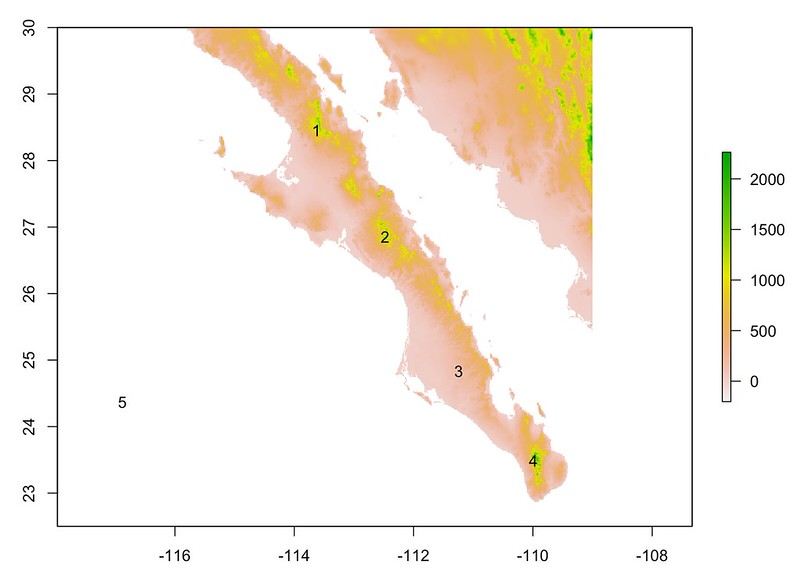
\includegraphics[keepaspectratio]{media/map_with_points.jpg}}

}

\caption{map with points}

\end{figure}%

Here are what the points look like.

\begin{Shaded}
\begin{Highlighting}[]
\NormalTok{points}
\end{Highlighting}
\end{Shaded}

\begin{verbatim}
          x        y value
1 -113.6292 28.45417   870
2 -112.4792 26.85417  1185
3 -111.2458 24.83750   135
4 -109.9958 23.48750  1145
\end{verbatim}

I'm going to rename the column names

\begin{Shaded}
\begin{Highlighting}[]
\NormalTok{points }\SpecialCharTok{\%\textgreater{}\%}
  \FunctionTok{transmute}\NormalTok{( }\AttributeTok{Longitude =}\NormalTok{ x,}
             \AttributeTok{Latitude =}\NormalTok{ y,}
             \AttributeTok{Value =}\NormalTok{ value) }\OtherTok{{-}\textgreater{}}\NormalTok{ sites}
\end{Highlighting}
\end{Shaded}

And then I can plot those points (using \texttt{geom\_point()}) onto our
background map.

\begin{Shaded}
\begin{Highlighting}[]
\NormalTok{baja\_map }\SpecialCharTok{+} 
  \FunctionTok{geom\_point}\NormalTok{( }\FunctionTok{aes}\NormalTok{(}\AttributeTok{x =}\NormalTok{ Longitude,}
                  \AttributeTok{y =}\NormalTok{ Latitude, }
                  \AttributeTok{size =}\NormalTok{ Value), }\AttributeTok{data=}\NormalTok{sites, }\AttributeTok{color=}\StringTok{"red"}\NormalTok{) }
\end{Highlighting}
\end{Shaded}

\pandocbounded{
\includegraphics[keepaspectratio]{narrative_rasters_files/figure-pdf/unnamed-chunk-25-1.pdf}}

Mexellent!

\section{Reprojecting Rasters}\label{reprojecting-rasters}

Just like points, we can reproject the entire raster using the
\texttt{projectRaster} function. HJere I am going to project the raster
into UTM Zone 12N, a common projection for this part of
\href{https://epsg.io/6367}{Mexico from epsg.io}.

Unfortunatly, the \texttt{raster} library does not use epsg codes so
we'll have to use the large description of that projection. See the
\href{https://epsg.io/6367}{page} for this projection and scroll down to
the proj.4 definition.

\begin{Shaded}
\begin{Highlighting}[]
\NormalTok{new.proj }\OtherTok{\textless{}{-}} \StringTok{"+proj=utm +zone=12 +ellps=GRS80 +towgs84=0,0,0,0,0,0,0 +units=m +no\_defs "}
\end{Highlighting}
\end{Shaded}

Copy this into a character variable and then use the
\texttt{projectRaster()} function and assign that new value as the
\texttt{CRS}.

\begin{Shaded}
\begin{Highlighting}[]
\NormalTok{alt.utm }\OtherTok{\textless{}{-}} \FunctionTok{projectRaster}\NormalTok{( alt, }\AttributeTok{crs=}\NormalTok{new.proj)}
\FunctionTok{plot}\NormalTok{( alt.utm, }\AttributeTok{xlab=}\StringTok{"Easting"}\NormalTok{, }\AttributeTok{ylab=}\StringTok{"Northing"}\NormalTok{ )}
\end{Highlighting}
\end{Shaded}

\pandocbounded{
\includegraphics[keepaspectratio]{narrative_rasters_files/figure-pdf/unnamed-chunk-27-1.pdf}}

Easy.

\section{Raster Operations}\label{raster-operations}

OK, so now we can make and show a raster but what about doing some
operations? A raster is just a matrix \emph{decorated} with more
geospatial information. This allows us to do normal \texttt{R} like data
manipulations on the underlying data.

Consider the following question.

\begin{quote}
What are the parts of Baja California that are within 100m of the
elevation of site named \emph{San Francisquito} (\texttt{sfran})?
\end{quote}

To answer this, we have the following general outline of operations.

\begin{enumerate}
\def\labelenumi{\arabic{enumi}.}
\tightlist
\item
  Find the coordinates of the site named \texttt{sfran}\\
\item
  Extract the elevation from the \texttt{alt} raster that is within 100m
  (+/-) of that site.
\item
  Plot the whole baja data as a background\\
\item
  Overlay all the locations within that elevation band.
\end{enumerate}

To do this we will use both the \texttt{alt} and the \texttt{beetles}
data objects.

First, we find out the coordinates of the site.

\begin{Shaded}
\begin{Highlighting}[]
\NormalTok{sfran }\OtherTok{\textless{}{-}}\NormalTok{ beetles}\SpecialCharTok{$}\NormalTok{geometry[ beetles}\SpecialCharTok{$}\NormalTok{Site }\SpecialCharTok{==} \StringTok{"sfran"}\NormalTok{]}
\NormalTok{sfran}
\end{Highlighting}
\end{Shaded}

\begin{verbatim}
Geometry set for 1 feature 
Geometry type: POINT
Dimension:     XY
Bounding box:  xmin: -112.964 ymin: 27.3632 xmax: -112.964 ymax: 27.3632
Geodetic CRS:  WGS 84
\end{verbatim}

\begin{verbatim}
POINT (-112.964 27.3632)
\end{verbatim}

Now, we need to figure out what the value of elevation in the
\texttt{alt} raster is at this site. This can be done with the
\texttt{extract()} function from the \texttt{raster} library.

\textbf{However}, the this function doesn't work directly with
\texttt{sf} objects so we need to cast it into a \texttt{Spatial}
object\footnote{Pielou EC, (1984) The interpretation of ecological data:
  A primer on classification and ordination. 288pg. ISBN:
  \href{https://www.wiley.com/en-us/The+Interpretation+of+Ecological+Data\%3A+A+Primer+on+Classification+and+Ordination-p-9780471889502}{978-0-471-88950-2}}.
Fortunatly, that is a pretty easy coercion.

\begin{Shaded}
\begin{Highlighting}[]
\NormalTok{raster}\SpecialCharTok{::}\FunctionTok{extract}\NormalTok{(alt, }\FunctionTok{as}\NormalTok{(sfran,}\StringTok{"Spatial"}\NormalTok{) ) }
\end{Highlighting}
\end{Shaded}

\begin{verbatim}
[1] 305
\end{verbatim}

\textbf{Warning:} in the above code, I used the function
\texttt{extract()} to extract the data from the \texttt{alt} raster for
the coordinate of the target locale. However, there is also an
\texttt{extract()} function that has been brought in from the
\texttt{dplyr} library (as part of \texttt{tidyverse}). In this file, I
loaded \texttt{library(raster)} before \texttt{library(tidyverse)} and
as such the \texttt{dplyr::extract()} function has overridden the one
from \texttt{raster}---they cannot \emph{both} be available. As a
consequence, I use the full name of the function with
\texttt{package::function} when I call it as \texttt{raster::extract()}
to remove all ambiguity. If I had not, I got a message saying something
like,
\texttt{Error\ in\ UseMethod("extract\_")\ :\ no\ applicable\ method\ for\ \textquotesingle{}extract\_\textquotesingle{}\ applied\ to\ an\ object\ of\ class\ "c(\textquotesingle{}RasterLayer\textquotesingle{},\ \textquotesingle{}Raster\textquotesingle{},\ \textquotesingle{}BasicRaster\textquotesingle{})"}.
Now, I know there is an \texttt{extract()} function in \texttt{raster}
so this is the \textbf{dead giveaway} that it has been overwritten by a
subsequent library call.

\subsection{Option 1 - Manipulate the
Raster}\label{option-1---manipulate-the-raster}

To work on a raster directly, we can access the values within it using
the \texttt{values()} function (I know, these statistican/programmers
are quite cleaver).

So, to make a copy and make only the values that are +/- 100m of
\texttt{sfran} we can.

\begin{Shaded}
\begin{Highlighting}[]
\NormalTok{alt\_band }\OtherTok{\textless{}{-}}\NormalTok{ alt}
\FunctionTok{values}\NormalTok{( alt\_band )[ }\FunctionTok{values}\NormalTok{(alt\_band) }\SpecialCharTok{\textless{}=} \DecValTok{205}\NormalTok{ ] }\OtherTok{\textless{}{-}} \ConstantTok{NA}
\FunctionTok{values}\NormalTok{( alt\_band )[ }\FunctionTok{values}\NormalTok{(alt\_band) }\SpecialCharTok{\textgreater{}=} \DecValTok{405}\NormalTok{ ] }\OtherTok{\textless{}{-}} \ConstantTok{NA}
\NormalTok{alt\_band}
\end{Highlighting}
\end{Shaded}

\begin{verbatim}
class      : RasterLayer 
dimensions : 960, 840, 806400  (nrow, ncol, ncell)
resolution : 0.008333333, 0.008333333  (x, y)
extent     : -116, -109, 22, 30  (xmin, xmax, ymin, ymax)
crs        : +proj=longlat +datum=WGS84 +no_defs 
source     : memory
names      : alt_22 
values     : 206, 404  (min, max)
\end{verbatim}

Then we can plot overlay plots of each (notice how I hid the legend for
the first \texttt{alt} raster).

\begin{Shaded}
\begin{Highlighting}[]
\FunctionTok{plot}\NormalTok{( alt, }\AttributeTok{col=}\StringTok{"gray"}\NormalTok{, }\AttributeTok{legend=}\ConstantTok{FALSE}\NormalTok{, }\AttributeTok{xlab=}\StringTok{"Longitude"}\NormalTok{, }\AttributeTok{ylab=}\StringTok{"Latitude"}\NormalTok{)}
\FunctionTok{plot}\NormalTok{( alt\_band, }\AttributeTok{add=}\ConstantTok{TRUE}\NormalTok{ )}
\end{Highlighting}
\end{Shaded}

\pandocbounded{
\includegraphics[keepaspectratio]{narrative_rasters_files/figure-pdf/unnamed-chunk-31-1.pdf}}

\subsection{Option 2 - Manipulate the Data
Frames}\label{option-2---manipulate-the-data-frames}

We can also proceed by relying upon the \texttt{data.frame} objects
representing the elevation. So let's go back to our the \texttt{alt.df}
object and use that in combination with a \texttt{filter} and plot both
\texttt{data.frame} objects (the outline of the landscape in gray and
the elevation range as a gradient). I then overlay the beetle data with
the ratios as sizes and label the locales with \texttt{ggrepel}. Notice
here that you can use the \texttt{sf::geometry} object from
\texttt{beetles} if you pass it through the \texttt{st\_coordinates}
function as a statistical tranform making it regular coordinates and not
\texttt{sf} objects (yes this is kind of a trick and hack but KEEP IT
HANDY!).

\begin{Shaded}
\begin{Highlighting}[]
\FunctionTok{library}\NormalTok{( ggrepel )}
\NormalTok{alt.df }\SpecialCharTok{\%\textgreater{}\%}
  \FunctionTok{filter}\NormalTok{( Elevation }\SpecialCharTok{\textgreater{}=} \DecValTok{205}\NormalTok{,}
\NormalTok{          Elevation }\SpecialCharTok{\textless{}=} \DecValTok{405}\NormalTok{) }\SpecialCharTok{\%\textgreater{}\%}
  \FunctionTok{ggplot}\NormalTok{() }\SpecialCharTok{+} 
  \FunctionTok{geom\_raster}\NormalTok{( }\FunctionTok{aes}\NormalTok{( }\AttributeTok{x =}\NormalTok{ Longitude,}
                    \AttributeTok{y =}\NormalTok{ Latitude),}
               \AttributeTok{fill =} \StringTok{"gray80"}\NormalTok{, }
               \AttributeTok{data=}\NormalTok{alt.df ) }\SpecialCharTok{+} 
  \FunctionTok{geom\_raster}\NormalTok{( }\FunctionTok{aes}\NormalTok{( }\AttributeTok{x =}\NormalTok{ Longitude,}
                    \AttributeTok{y =}\NormalTok{ Latitude, }
                    \AttributeTok{fill =}\NormalTok{ Elevation ) ) }\SpecialCharTok{+} 
  \FunctionTok{scale\_fill\_gradient2}\NormalTok{( }\AttributeTok{low =} \StringTok{"darkolivegreen"}\NormalTok{,}
                        \AttributeTok{mid =} \StringTok{"yellow"}\NormalTok{,}
                        \AttributeTok{high =} \StringTok{"brown"}\NormalTok{, }
                        \AttributeTok{midpoint =} \DecValTok{305}\NormalTok{ ) }\SpecialCharTok{+}
  \FunctionTok{geom\_sf}\NormalTok{( }\FunctionTok{aes}\NormalTok{(}\AttributeTok{size=}\NormalTok{MFRatio), }
           \AttributeTok{alpha=}\FloatTok{0.5}\NormalTok{, }
           \AttributeTok{color=}\StringTok{"dodgerblue3"}\NormalTok{, }
           \AttributeTok{data=}\NormalTok{beetles) }\SpecialCharTok{+}
  \FunctionTok{geom\_text\_repel}\NormalTok{( }\FunctionTok{aes}\NormalTok{( }\AttributeTok{label =}\NormalTok{ Site,}
                        \AttributeTok{geometry =}\NormalTok{ geometry),}
                   \AttributeTok{data =}\NormalTok{ beetles,}
                   \AttributeTok{stat =} \StringTok{"sf\_coordinates"}\NormalTok{, }
                   \AttributeTok{size =} \DecValTok{4}\NormalTok{, }
                   \AttributeTok{color =} \StringTok{"dodgerblue4"}\NormalTok{) }\SpecialCharTok{+} 
  \FunctionTok{coord\_sf}\NormalTok{() }\SpecialCharTok{+} 
  \FunctionTok{theme\_minimal}\NormalTok{() }
\end{Highlighting}
\end{Shaded}

\begin{verbatim}
Warning in st_point_on_surface.sfc(sf::st_zm(x)): st_point_on_surface may not
give correct results for longitude/latitude data
\end{verbatim}

\pandocbounded{
\includegraphics[keepaspectratio]{narrative_rasters_files/figure-pdf/unnamed-chunk-32-1.pdf}}

Very nice indeed.

\part{Statistical Models}

Here we examine some of the most common statistical approaches used and
how to integrate them into your analysis workflow.

\chapter{Correlations}\label{correlations}

\pandocbounded{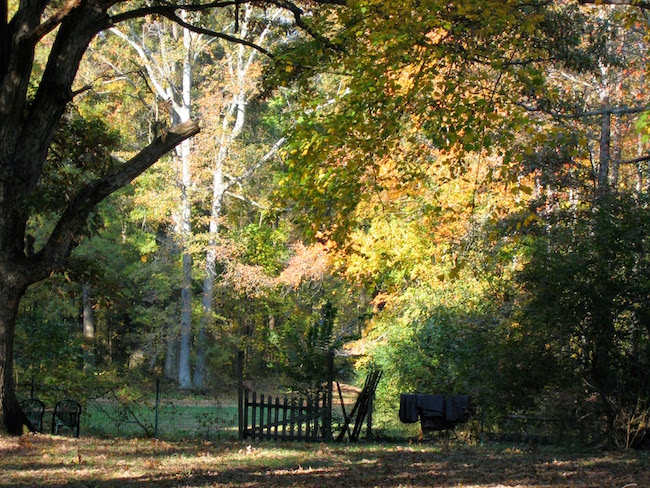
\includegraphics[keepaspectratio]{media/chapter_correlation.jpg}}

\begin{quote}
Correlation is a test to see if two variables change in a coordinate
fashion. However, this does not imply they are functionally linked or
causal in nature.
\end{quote}

\section{Lecture Materials}\label{lecture-materials-11}

\begin{quote}
\textbf{Lecture Slides:} Available interactively in the
\href{https://dyerlabteaching.github.io/Correlation/slides.html\#/title-slide}{online
version}
\end{quote}

\begin{figure}[H]

{\centering \pandocbounded{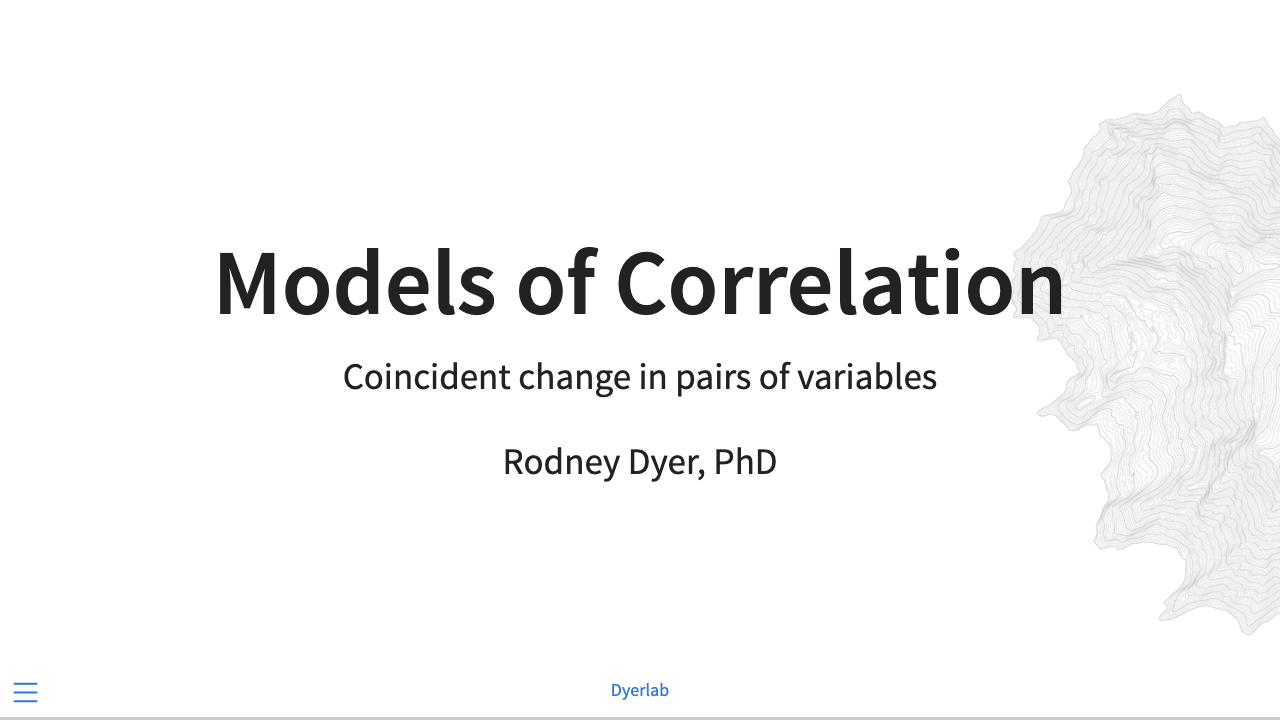
\includegraphics[keepaspectratio]{media/slides_correlation.png}}

}

\caption{Lecture Slides}

\end{figure}%

Consider the following data consisting of the the decade from 1999 -
2009 and recording the number of movies each year by the American Actor,
and cultural treasure, Mr.~Nicolas Cage (source IMDB).

\begin{figure}[H]

{\centering \pandocbounded{\includegraphics[keepaspectratio]{media/NicolasCage.png}}

}

\caption{Various roles played by the American actor, Mr.~Nicolas Cage.}

\end{figure}%

Also, let's look at the number of people who accidentally died by
falling into a swimming pool (source U.S. Centers for Disease Control)
during this same period.

\begin{Shaded}
\begin{Highlighting}[]
\NormalTok{df }\OtherTok{\textless{}{-}} \FunctionTok{data.frame}\NormalTok{( }\AttributeTok{Year =} \DecValTok{1999}\SpecialCharTok{:}\DecValTok{2009}\NormalTok{ )}
\NormalTok{df}\SpecialCharTok{$}\StringTok{\textasciigrave{}}\AttributeTok{Nicolas Cage Movies}\StringTok{\textasciigrave{}} \OtherTok{\textless{}{-}} \FunctionTok{c}\NormalTok{( }\DecValTok{2}\NormalTok{, }\DecValTok{2}\NormalTok{, }\DecValTok{2}\NormalTok{, }\DecValTok{3}\NormalTok{, }\DecValTok{1}\NormalTok{, }\DecValTok{1}\NormalTok{, }\DecValTok{2}\NormalTok{, }\DecValTok{3}\NormalTok{, }\DecValTok{4}\NormalTok{, }\DecValTok{1}\NormalTok{, }\DecValTok{4}\NormalTok{)}
\NormalTok{df}\SpecialCharTok{$}\StringTok{\textasciigrave{}}\AttributeTok{Drowning Deaths in Pools}\StringTok{\textasciigrave{}} \OtherTok{\textless{}{-}} \FunctionTok{c}\NormalTok{( }\DecValTok{109}\NormalTok{, }\DecValTok{102}\NormalTok{, }\DecValTok{102}\NormalTok{, }\DecValTok{98}\NormalTok{, }\DecValTok{85}\NormalTok{, }\DecValTok{95}\NormalTok{, }\DecValTok{96}\NormalTok{, }\DecValTok{98}\NormalTok{, }\DecValTok{123}\NormalTok{, }\DecValTok{94}\NormalTok{, }\DecValTok{102}\NormalTok{ ) }
\NormalTok{df}
\end{Highlighting}
\end{Shaded}

\begin{verbatim}
   Year Nicolas Cage Movies Drowning Deaths in Pools
1  1999                   2                      109
2  2000                   2                      102
3  2001                   2                      102
4  2002                   3                       98
5  2003                   1                       85
6  2004                   1                       95
7  2005                   2                       96
8  2006                   3                       98
9  2007                   4                      123
10 2008                   1                       94
11 2009                   4                      102
\end{verbatim}

If we look at these data by year, it does not look like there is much of
a trend (at least temporally). We've talked about the
\texttt{tidyr::pivot\_longer} approach to take data like this and
manipulate it. There is another way to do this using the
\texttt{reshape2} library uwing the function \texttt{melt()}. I
recommend you go take a look at that to see how this works as well. Both
are valid ways.

\begin{Shaded}
\begin{Highlighting}[]
\FunctionTok{library}\NormalTok{( tidyverse )}
\end{Highlighting}
\end{Shaded}

\begin{verbatim}
-- Attaching core tidyverse packages ------------------------ tidyverse 2.0.0 --
v dplyr     1.2.1     v readr     2.2.0
v forcats   1.0.1     v stringr   1.6.0
v ggplot2   4.0.2     v tibble    3.3.1
v lubridate 1.9.5     v tidyr     1.3.2
v purrr     1.2.1     
-- Conflicts ------------------------------------------ tidyverse_conflicts() --
x dplyr::filter() masks stats::filter()
x dplyr::lag()    masks stats::lag()
i Use the conflicted package (<http://conflicted.r-lib.org/>) to force all conflicts to become errors
\end{verbatim}

\begin{Shaded}
\begin{Highlighting}[]
\FunctionTok{library}\NormalTok{( reshape2 )}
\end{Highlighting}
\end{Shaded}

\begin{verbatim}

Attaching package: 'reshape2'

The following object is masked from 'package:tidyr':

    smiths
\end{verbatim}

\begin{Shaded}
\begin{Highlighting}[]
\NormalTok{df }\SpecialCharTok{|\textgreater{}}
  \FunctionTok{melt}\NormalTok{( }\AttributeTok{id =} \StringTok{"Year"}\NormalTok{ ) }
\end{Highlighting}
\end{Shaded}

\begin{verbatim}
   Year                 variable value
1  1999      Nicolas Cage Movies     2
2  2000      Nicolas Cage Movies     2
3  2001      Nicolas Cage Movies     2
4  2002      Nicolas Cage Movies     3
5  2003      Nicolas Cage Movies     1
6  2004      Nicolas Cage Movies     1
7  2005      Nicolas Cage Movies     2
8  2006      Nicolas Cage Movies     3
9  2007      Nicolas Cage Movies     4
10 2008      Nicolas Cage Movies     1
11 2009      Nicolas Cage Movies     4
12 1999 Drowning Deaths in Pools   109
13 2000 Drowning Deaths in Pools   102
14 2001 Drowning Deaths in Pools   102
15 2002 Drowning Deaths in Pools    98
16 2003 Drowning Deaths in Pools    85
17 2004 Drowning Deaths in Pools    95
18 2005 Drowning Deaths in Pools    96
19 2006 Drowning Deaths in Pools    98
20 2007 Drowning Deaths in Pools   123
21 2008 Drowning Deaths in Pools    94
22 2009 Drowning Deaths in Pools   102
\end{verbatim}

Let's plot this to see \texttt{through\ time} variation.

\begin{Shaded}
\begin{Highlighting}[]
\NormalTok{df }\SpecialCharTok{|\textgreater{}}
  \FunctionTok{melt}\NormalTok{( }\AttributeTok{id =} \StringTok{"Year"}\NormalTok{ ) }\SpecialCharTok{|\textgreater{}} 
  \FunctionTok{ggplot}\NormalTok{( }\FunctionTok{aes}\NormalTok{( Year, value, }\AttributeTok{color =}\NormalTok{ variable) ) }\SpecialCharTok{+} 
  \FunctionTok{geom\_line}\NormalTok{()  }\SpecialCharTok{+}
  \FunctionTok{geom\_point}\NormalTok{() }
\end{Highlighting}
\end{Shaded}

\pandocbounded{
\includegraphics[keepaspectratio]{narrative_correlation_files/figure-pdf/unnamed-chunk-3-1.pdf}}

However, if we look at the two variables together we see an entirely
different thing.

\begin{Shaded}
\begin{Highlighting}[]
\NormalTok{df }\SpecialCharTok{|\textgreater{}}
  \FunctionTok{ggplot}\NormalTok{( }\FunctionTok{aes}\NormalTok{(}\StringTok{\textasciigrave{}}\AttributeTok{Nicolas Cage Movies}\StringTok{\textasciigrave{}}\NormalTok{, }
              \StringTok{\textasciigrave{}}\AttributeTok{Drowning Deaths in Pools}\StringTok{\textasciigrave{}}\NormalTok{ ) ) }\SpecialCharTok{+}
  \FunctionTok{geom\_point}\NormalTok{( }\AttributeTok{size=}\DecValTok{2}\NormalTok{ ) }\SpecialCharTok{+} 
  \FunctionTok{stat\_smooth}\NormalTok{( }\AttributeTok{formula=}\NormalTok{y }\SpecialCharTok{\textasciitilde{}}\NormalTok{ x,}
               \AttributeTok{method=}\StringTok{\textquotesingle{}lm\textquotesingle{}}\NormalTok{,}
               \AttributeTok{se=}\ConstantTok{FALSE}\NormalTok{,}
               \AttributeTok{color =} \StringTok{"red"}\NormalTok{) }\SpecialCharTok{+}
  \FunctionTok{geom\_text}\NormalTok{( }\FunctionTok{aes}\NormalTok{(}\AttributeTok{x=}\FloatTok{1.5}\NormalTok{,}
                 \AttributeTok{y=}\DecValTok{115}\NormalTok{,}
                 \AttributeTok{label =} \FunctionTok{paste}\NormalTok{( }\StringTok{"Correlation = "}\NormalTok{, }
                                \FunctionTok{format}\NormalTok{( }\FunctionTok{cor}\NormalTok{( df[,}\DecValTok{2}\NormalTok{],}
\NormalTok{                                             df[,}\DecValTok{3}\NormalTok{]), }
                                        \AttributeTok{digits=}\DecValTok{3}\NormalTok{) ) ) )}
\end{Highlighting}
\end{Shaded}

\begin{verbatim}
Warning in geom_text(aes(x = 1.5, y = 115, label = paste("Correlation = ", : All aesthetics have length 1, but the data has 11 rows.
i Please consider using `annotate()` or provide this layer with data containing
  a single row.
\end{verbatim}

\pandocbounded{
\includegraphics[keepaspectratio]{narrative_correlation_files/figure-pdf/unnamed-chunk-4-1.pdf}}

And in fact, if we run the statistical test on these data.

\begin{Shaded}
\begin{Highlighting}[]
\FunctionTok{cor.test}\NormalTok{( df}\SpecialCharTok{$}\StringTok{\textasciigrave{}}\AttributeTok{Nicolas Cage Movies}\StringTok{\textasciigrave{}}\NormalTok{, df}\SpecialCharTok{$}\StringTok{\textasciigrave{}}\AttributeTok{Drowning Deaths in Pools}\StringTok{\textasciigrave{}}\NormalTok{) }\OtherTok{{-}\textgreater{}}\NormalTok{ fit.cage}
\NormalTok{fit.cage}
\end{Highlighting}
\end{Shaded}

\begin{verbatim}

    Pearson's product-moment correlation

data:  df$`Nicolas Cage Movies` and df$`Drowning Deaths in Pools`
t = 2.6785, df = 9, p-value = 0.02527
alternative hypothesis: true correlation is not equal to 0
95 percent confidence interval:
 0.1101273 0.9045101
sample estimates:
      cor 
0.6660043 
\end{verbatim}

We do in fact see a significant (P = 0.0253) relationship.

Now, do we think that because Nicolas Cage makes more movies people are
dying at an increased rate? No.~These are spurious correlations, though
do prove a point about causation.

\section{Some New Data}\label{some-new-data}

For this topic, I thought I would turn to a bit of a more digestible set
of data---data describing beer styles! There is a new CSV data set on
the GitHub site located at the following URL.

\begin{Shaded}
\begin{Highlighting}[]
\NormalTok{beer\_url }\OtherTok{\textless{}{-}} \StringTok{"https://raw.githubusercontent.com/dyerlab/ENVS{-}Lectures/master/data/Beer\_Styles.csv"}
\NormalTok{beer }\OtherTok{\textless{}{-}} \FunctionTok{read\_csv}\NormalTok{( beer\_url )}
\end{Highlighting}
\end{Shaded}

\begin{verbatim}
Rows: 100 Columns: 12
-- Column specification --------------------------------------------------------
Delimiter: ","
chr  (2): Styles, Yeast
dbl (10): ABV_Min, ABV_Max, IBU_Min, IBU_Max, SRM_Min, SRM_Max, OG_Min, OG_M...

i Use `spec()` to retrieve the full column specification for this data.
i Specify the column types or set `show_col_types = FALSE` to quiet this message.
\end{verbatim}

\begin{Shaded}
\begin{Highlighting}[]
\FunctionTok{summary}\NormalTok{( beer )}
\end{Highlighting}
\end{Shaded}

\begin{verbatim}
    Styles             Yeast              ABV_Min         ABV_Max      
 Length:100         Length:100         Min.   :2.400   Min.   : 3.200  
 Class :character   Class :character   1st Qu.:4.200   1st Qu.: 5.475  
 Mode  :character   Mode  :character   Median :4.600   Median : 6.000  
                                       Mean   :4.947   Mean   : 6.768  
                                       3rd Qu.:5.500   3rd Qu.: 8.000  
                                       Max.   :9.000   Max.   :14.000  
    IBU_Min         IBU_Max          SRM_Min         SRM_Max     
 Min.   : 0.00   Min.   :  8.00   Min.   : 2.00   Min.   : 3.00  
 1st Qu.:15.00   1st Qu.: 25.00   1st Qu.: 3.50   1st Qu.: 7.00  
 Median :20.00   Median : 35.00   Median : 8.00   Median :17.00  
 Mean   :21.97   Mean   : 38.98   Mean   : 9.82   Mean   :17.76  
 3rd Qu.:25.00   3rd Qu.: 45.00   3rd Qu.:14.00   3rd Qu.:22.00  
 Max.   :60.00   Max.   :120.00   Max.   :30.00   Max.   :40.00  
     OG_Min          OG_Max          FG_Min          FG_Max     
 Min.   :1.026   Min.   :1.032   Min.   :0.998   Min.   :1.006  
 1st Qu.:1.040   1st Qu.:1.052   1st Qu.:1.008   1st Qu.:1.012  
 Median :1.046   Median :1.060   Median :1.010   Median :1.015  
 Mean   :1.049   Mean   :1.065   Mean   :1.009   Mean   :1.016  
 3rd Qu.:1.056   3rd Qu.:1.075   3rd Qu.:1.010   3rd Qu.:1.018  
 Max.   :1.080   Max.   :1.130   Max.   :1.020   Max.   :1.040  
\end{verbatim}

The data consist of the following categories of data. For all but he
first two columns of data, a range is given for the appropriate values
for each style with \texttt{Min} and \texttt{Max} values.

\begin{itemize}
\tightlist
\item
  \emph{Styles} - The official name of the beer style. Yes, there is an
  international standard that is officiated by the
  \href{https://bjcp.org/}{Beer Judge Certification Program}.
\item
  \emph{Yeast Type} - The species of yeast most commonly used for
  fermenation, consists of top fermenting Ale yeasts and bottom
  fermenting Lager yeasts.\\
\item
  \emph{ABV} - The amount of alcohol in the finished beer as a
  percentage of the volume. This is a non-negative numerical value.
\item
  \emph{IBU} - The `International Bitterness Unit' which roughly
  measures the amont of \(\alpha\)-acids (asymptotically) added to the
  beer by the hops. This is a non-negative numerical value, with higher
  values indicating more bitter beer, though human ability to taste
  increasingly bitter beer is asymptotic.
\item
  \emph{SRM} - The Standard Reference Method calibration measuring the
  color of the finished beer. This is a non-negative integer going from
  1 - 40 (light straw color - dark opaque).
\item
  \emph{OG} - The amount of dissolved sugars in the wort (the pre-beer
  liquid prior to putting in yeast and the initiation of fermentation),
  relative to pure water. This is a measurement `relative' to water,
  which is 1.0. Values less than 1.0 have lower liquid densities than
  pure water and those greater than 1.0 have more dissolved sugars than
  pure water.
\item
  \emph{FG} - The amount of dissolved sugars in the beer after
  fermentation has been completed. Same as above but the difference in
  \emph{OG} and \emph{FG} can tell us what the \emph{ABV} should be.
  Hihger \emph{FG} beers are more sweet and have more body than lower
  \emph{OG} beers (which may appear to have a cleaner, drier, mouth
  feel---yes that is a real term as well).
\end{itemize}

As we talk about correlations, we will use these as examples.

\section{Parameters \& Estimates}\label{parameters-estimates}

In statistics, we have two kinds of entities, parameters and estimates,
which are dualities of each other. The \texttt{TRUE} mean of a set of
data is referred to by \(\mu\) whereas the mean of the data we measured
is referred to as \(\bar{x}\). The greek version is the \emph{idealized}
value for the parameter, something that we are striving to find the real
estimate of. However, as a Frequentist, we can never actually get to
that parameter (remember the actual population of data is infinite but
we can only sample a small amount of it) and when we talk about the data
associated with what we collect, we refer to it as a estimate and use
normal variable names.

\section{Parametric Assumptions}\label{parametric-assumptions}

For much of the statistics we use, there are underlying assumptions
about the form of the data that we shold look at.

\subsection{Testing for Normality.}\label{testing-for-normality.}

\begin{quote}
The data can be estimated by a normal density function, or at least can
be transformed into data that is reasonably normal in distribution.
\end{quote}

The normal distribution function is defined as:

\[
f(x) = \frac{1}{\sigma\sqrt{2\pi}}e^{-\frac{1}{2}(\frac{x - \mu}{\sigma})}
\]

where \(\mu\) and \(\sigma\) are the true value of the underlying mean
and standard deviation. This distribution is denoted as
\(N(\mu,\sigma)\) and the differences in the mean value (\(\mu\)) and
the variation measured by the standard deviation (\(\sigma\)) are shown
below for \(N(0,1)\), \(N(0,5)\), and \(N(10,1)\).

\begin{Shaded}
\begin{Highlighting}[]
\NormalTok{N }\OtherTok{\textless{}{-}} \DecValTok{1000}
\FunctionTok{data.frame}\NormalTok{( }\AttributeTok{Distribution =} \FunctionTok{rep}\NormalTok{(}\FunctionTok{c}\NormalTok{(}\StringTok{"N(0,1)"}\NormalTok{,}\StringTok{"N(10,1)"}\NormalTok{, }\StringTok{"N(0,5)"}\NormalTok{), }\AttributeTok{each=}\NormalTok{N ),}
            \AttributeTok{Data =} \FunctionTok{c}\NormalTok{( }\FunctionTok{rnorm}\NormalTok{(N,}\DecValTok{0}\NormalTok{,}\DecValTok{1}\NormalTok{),}
                      \FunctionTok{rnorm}\NormalTok{(N,}\DecValTok{10}\NormalTok{,}\DecValTok{1}\NormalTok{),}
                      \FunctionTok{rnorm}\NormalTok{(N,}\DecValTok{0}\NormalTok{,}\DecValTok{5}\NormalTok{) ) ) }\SpecialCharTok{|\textgreater{}}
  \FunctionTok{ggplot}\NormalTok{( }\FunctionTok{aes}\NormalTok{( Data ) ) }\SpecialCharTok{+} 
  \FunctionTok{geom\_histogram}\NormalTok{( }\AttributeTok{alpha=}\FloatTok{0.75}\NormalTok{, }
                  \AttributeTok{bins =} \DecValTok{50}\NormalTok{) }\SpecialCharTok{+} 
  \FunctionTok{facet\_grid}\NormalTok{(Distribution }\SpecialCharTok{\textasciitilde{}}\NormalTok{.)}
\end{Highlighting}
\end{Shaded}

\pandocbounded{
\includegraphics[keepaspectratio]{narrative_correlation_files/figure-pdf/unnamed-chunk-7-1.pdf}}

There are a couple of ways to look at our data to see if they can be
considered as normal. First, visually we can plot the theoretical
(parameter) quantiles of the data against the sample quantiles using the
\texttt{qqnorm()} plot. What this does is sort the data by expectation
and observation and plot them and if the data are normal, then they
should roughly be in a straight line. The \texttt{qqline()} function
shows the expected line (n.b., this is another one of those things where
you have to run the whole chunk to get both points and lines on the same
graph if you are working in Markdown).

\begin{Shaded}
\begin{Highlighting}[]
\FunctionTok{qqnorm}\NormalTok{( beer}\SpecialCharTok{$}\NormalTok{ABV\_Min )}
\FunctionTok{qqline}\NormalTok{( beer}\SpecialCharTok{$}\NormalTok{ABV\_Min, }\AttributeTok{col=}\StringTok{"red"}\NormalTok{)}
\end{Highlighting}
\end{Shaded}

\pandocbounded{
\includegraphics[keepaspectratio]{narrative_correlation_files/figure-pdf/unnamed-chunk-8-1.pdf}}

So, what we commonly see is most of the data falling along the line
throughout the middle portion of the distribution and then deviating
around the edges. What this does not do is give you a statistic to test
to see if we can reject the hypothesis \(H_O: Data\;is\;normal\). For
this, we can use the Shapiro-Wilkes Normality test which produces the
statistic:

\[
W = \frac{\left(\sum_{i=1}^Na_iR_{x_i}\right)^2}{\sum_{i=1}^N(x_i - \bar{x})^2}
\]

where \(N\) is the number of samples, \(a_i\) is a standardizing
coeeficient, \(x_i\) is the \(i^{th}\) value of \(x\), \(\bar{x}\) is
the mean of the observed values, and \(R_{x_i}\) is the rank of the
\(x_i^{th}\) observation.

\begin{Shaded}
\begin{Highlighting}[]
\FunctionTok{shapiro.test}\NormalTok{( beer}\SpecialCharTok{$}\NormalTok{ABV\_Min )}
\end{Highlighting}
\end{Shaded}

\begin{verbatim}

    Shapiro-Wilk normality test

data:  beer$ABV_Min
W = 0.94595, p-value = 0.0004532
\end{verbatim}

Rejection of the null hypothesis (e.g., a small \texttt{p-value} from
the test) indicates that the data \emph{are not} to be considered as
coming from a normal distribution. So, for the \texttt{ABV\_Min} data
above, it appears that it is not actually normally distributed. So what
do we do?

\subsection{Transformations}\label{transformations}

If the data are not normal, we can look towards trying to see if we can
transform it to a normally distributed variable. There are a lot of

\emph{Studentized Data} - One way to standardize the data is to make it
have a mean of 0.0 and a standard deviation of 1.0. To do this, we
subtract the \texttt{mean()} and divide by the \texttt{sd()}.

\begin{Shaded}
\begin{Highlighting}[]
\NormalTok{x }\OtherTok{\textless{}{-}}\NormalTok{ beer}\SpecialCharTok{$}\NormalTok{ABV\_Min }
\NormalTok{x.std }\OtherTok{\textless{}{-}}\NormalTok{ (x }\SpecialCharTok{{-}} \FunctionTok{mean}\NormalTok{(x)) }\SpecialCharTok{/} \FunctionTok{sd}\NormalTok{( x )}
\end{Highlighting}
\end{Shaded}

There are times when this can be a nice way to compare the

\emph{Box Cox} - In 1964, Box \& Cox defined a \emph{family} of
transformations known as the Box/Cox. This family is defined by a single
parameter, \(\lambda\), whose value may vary depending upon the data.
The original data, \(x\), is then transformed using the following
relationship

\[
\tilde{x} = \frac{x^\lambda - 1}{\lambda}
\]

\textbf{As long as \(\lambda \ne 0\) (else we would be dividing by zero,
which is not a good thing)!}

One way to use this transformation is to look at a range of values for
\(\lambda\) and determine if the transformation

\begin{Shaded}
\begin{Highlighting}[]
\NormalTok{test\_boxcox }\OtherTok{\textless{}{-}} \ControlFlowTok{function}\NormalTok{( x, }\AttributeTok{lambdas =} \FunctionTok{seq}\NormalTok{(}\SpecialCharTok{{-}}\FloatTok{1.1}\NormalTok{, }\FloatTok{1.1}\NormalTok{, }\AttributeTok{by =} \FloatTok{0.015}\NormalTok{) ) \{}
\NormalTok{  ret }\OtherTok{\textless{}{-}} \FunctionTok{data.frame}\NormalTok{( }\AttributeTok{Lambda =}\NormalTok{ lambdas,}
                     \AttributeTok{W =} \ConstantTok{NA}\NormalTok{,}
                     \AttributeTok{P =} \ConstantTok{NA}\NormalTok{)}
  
  \ControlFlowTok{for}\NormalTok{( lambda }\ControlFlowTok{in}\NormalTok{ lambdas ) \{}
\NormalTok{    x.tilde }\OtherTok{\textless{}{-}}\NormalTok{ (x}\SpecialCharTok{\^{}}\NormalTok{lambda }\SpecialCharTok{{-}} \DecValTok{1}\NormalTok{) }\SpecialCharTok{/}\NormalTok{ lambda   }
\NormalTok{    w }\OtherTok{\textless{}{-}} \FunctionTok{shapiro.test}\NormalTok{( x.tilde )}
\NormalTok{    ret}\SpecialCharTok{$}\NormalTok{W[ ret}\SpecialCharTok{$}\NormalTok{Lambda }\SpecialCharTok{==}\NormalTok{ lambda ] }\OtherTok{\textless{}{-}}\NormalTok{ w}\SpecialCharTok{$}\NormalTok{statistic}
\NormalTok{    ret}\SpecialCharTok{$}\NormalTok{P[ ret}\SpecialCharTok{$}\NormalTok{Lambda }\SpecialCharTok{==}\NormalTok{ lambda ] }\OtherTok{\textless{}{-}}\NormalTok{ w}\SpecialCharTok{$}\NormalTok{p.value}
\NormalTok{  \}}
  
  \FunctionTok{return}\NormalTok{( ret )}
\NormalTok{\}}

\NormalTok{vals }\OtherTok{\textless{}{-}} \FunctionTok{test\_boxcox}\NormalTok{( beer}\SpecialCharTok{$}\NormalTok{ABV\_Min ) }


\NormalTok{vals }\SpecialCharTok{|\textgreater{}}
  \FunctionTok{ggplot}\NormalTok{( }\FunctionTok{aes}\NormalTok{(Lambda, P) ) }\SpecialCharTok{+} 
  \FunctionTok{geom\_line}\NormalTok{() }\SpecialCharTok{+} 
  \FunctionTok{ylab}\NormalTok{(}\StringTok{"P{-}Value"}\NormalTok{)}
\end{Highlighting}
\end{Shaded}

\pandocbounded{
\includegraphics[keepaspectratio]{narrative_correlation_files/figure-pdf/unnamed-chunk-11-1.pdf}}

So if you look at this plot, it shows the P-value of the Shapiro-Wilkes
test across a range of values. Depending upon the level of rigor, this
approaches the \(\alpha = 0.05\) value closest at:

\begin{Shaded}
\begin{Highlighting}[]
\NormalTok{vals[ }\FunctionTok{which}\NormalTok{(vals}\SpecialCharTok{$}\NormalTok{P }\SpecialCharTok{==} \FunctionTok{max}\NormalTok{( vals}\SpecialCharTok{$}\NormalTok{P)),]}
\end{Highlighting}
\end{Shaded}

\begin{verbatim}
   Lambda        W          P
82  0.115 0.973805 0.04351988
\end{verbatim}

with \(\lambda = 0.115\) and a \(P = 0.044\).

\emph{Arc-Sine Square Root} When dealing with fractions, it is common
that they do not behave very well when they are very close to 0.0 or
1.0. One of the common transformations to use with these kinds of data
is the arc-sin square root transformation. For us, the ABV columns in
the data is a percentage (but listed in numerical form as percent not as
fraction). So to transform it we can do the following.

\begin{Shaded}
\begin{Highlighting}[]
\NormalTok{abv }\OtherTok{\textless{}{-}}\NormalTok{ beer}\SpecialCharTok{$}\NormalTok{ABV\_Min }\SpecialCharTok{/} \FloatTok{100.0}
\FunctionTok{asin}\NormalTok{( }\FunctionTok{sqrt}\NormalTok{( abv ) ) }\OtherTok{{-}\textgreater{}}\NormalTok{ abv}\FloatTok{.1}
\FunctionTok{shapiro.test}\NormalTok{( abv}\FloatTok{.1}\NormalTok{)}
\end{Highlighting}
\end{Shaded}

\begin{verbatim}

    Shapiro-Wilk normality test

data:  abv.1
W = 0.96746, p-value = 0.01418
\end{verbatim}

\section{Equal Variance}\label{equal-variance}

Another parametric assumption is the equality of variance across a range
of the data. This means, for example, that the variance from one part of
the experiment should not be different than the variance in samples from
another portion of data. We will return to this when we evaluate
regression models.

\section{Independence of Data}\label{independence-of-data}

The samples you collect, and the way that you design your experiments
are most important to ensure that your data are individually
independent. You need to think about this very carefully as you design
your experiments.

\chapter{Correlation Tests}\label{correlation-tests}

The following types of correlation statistics are a sample of the most
common approaches.

\section{Parametric Test: Pearson Product Moment
Correlations}\label{parametric-test-pearson-product-moment-correlations}

By far, the most common correlation statistic we see is the Pearson
Product Moment Correlation, denoted as \(\rho\). For two variables,
\(x\) and \(y\), the correlation parameter is estimated as:

\[
\rho = \frac{\sum_{i=1}^N(x_i - \bar{x})(y_i - \bar{y})}{\sqrt{\sum_{i=1}^N(x_i - \bar{x})^2}\sqrt{\sum_{i=1}^N(y_i - \bar{y})^2}}
\]

The values of these data fall wihtin the range of:
\(-1 \le \rho \le +1\) with negative values indicating that when one
variable goes up, the other goes down. Positive values of a correlation
indicate that both variable change systematically in the same direction
(e.g., both up or both down).

Here are some examples of the distribution of two variables and their
associated correlation coefficient.

\begin{figure}[H]

{\centering \pandocbounded{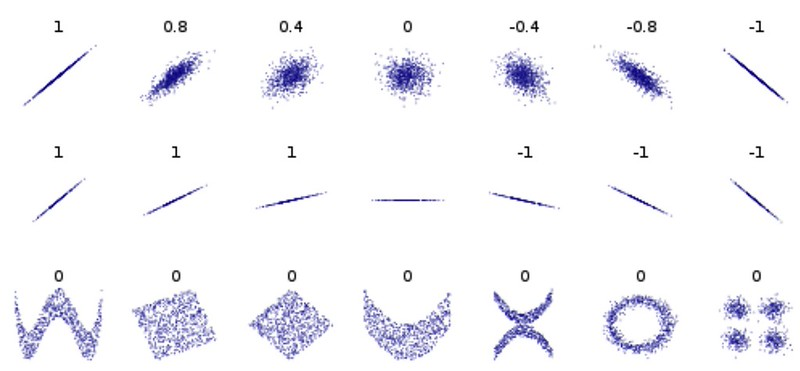
\includegraphics[keepaspectratio]{media/correlation_data.jpg}}

}

\caption{\emph{Figure 1: Data and associated correlation statistics.}}

\end{figure}%

Significance testing for a correlation such as \(\rho\) determine the
extent to which we thing the value of is deviant from zero. The Null
Hypothesis is \(H_O: \rho \ne 0\) and can be evaluated using the
Student's t.test. With large enough sample sizes, it can be approximated
by:

\[
t = r \frac{N-2}{1-r^2}
\]

However, we should probably rely upon \texttt{R} to look up the critical
values of the statistic.

The default value for \texttt{cor.test()} is the Pearson. Here is an
example of its use and the output that we've seen before.

\begin{Shaded}
\begin{Highlighting}[]
\FunctionTok{cor.test}\NormalTok{( beer}\SpecialCharTok{$}\NormalTok{OG\_Max, beer}\SpecialCharTok{$}\NormalTok{FG\_Max ) }\OtherTok{{-}\textgreater{}}\NormalTok{ OG.FG.pearson}
\NormalTok{OG.FG.pearson}
\end{Highlighting}
\end{Shaded}

\begin{verbatim}

    Pearson's product-moment correlation

data:  beer$OG_Max and beer$FG_Max
t = 15.168, df = 98, p-value < 2.2e-16
alternative hypothesis: true correlation is not equal to 0
95 percent confidence interval:
 0.7671910 0.8878064
sample estimates:
      cor 
0.8374184 
\end{verbatim}

Of particular note are the components associated with the results object
that allows you to gain access to specifics for any analysis.

\begin{Shaded}
\begin{Highlighting}[]
\FunctionTok{names}\NormalTok{( OG.FG.pearson )}
\end{Highlighting}
\end{Shaded}

\begin{verbatim}
[1] "statistic"   "parameter"   "p.value"     "estimate"    "null.value" 
[6] "alternative" "method"      "data.name"   "conf.int"   
\end{verbatim}

\section{Non-Parametric Test: Spearman's
Rho}\label{non-parametric-test-spearmans-rho}

Another way to de a correlation test that does not rely upon parametric
assumptions is to use non-parametric approaches. Most non-parametric
tests are based upon ranks of the data rather than the assumption of
normality of the data that is necessary for the Pearson Product Moment
statistic. One of the constraints for non-parametric statistics is that
they are often evaluated for probability based upon permutations.

The form of the estimator for this is almost identical to that of the
Pearson statistic except that instead of the raw data, we are replacing
values with the ranks of each value instead. In doing so, there is a
loss of the breadth of the raw data since we are just using ranks, and
if the underlying data are poorly behaved because of outliers or other
issues, this takes care of it.

\[
\rho_{Spearman} = \frac{ \sum_{i=1}^N(R_{x_i} - \bar{R_{x}})(R_{y_i} - \bar{R_{y}})}{\sqrt{\sum_{i=1}^N(R_{x_i} - \bar{R_{x}})^2}\sqrt{\sum_{i=1}^N(R_{y_i} - \bar{R_{y}})^2}}
\]

With the same data, it does provide potentially different estimates of
the amount of correlation between the variables.

\begin{Shaded}
\begin{Highlighting}[]
\NormalTok{OG.FG.spearman }\OtherTok{\textless{}{-}} \FunctionTok{cor.test}\NormalTok{( beer}\SpecialCharTok{$}\NormalTok{OG\_Max, beer}\SpecialCharTok{$}\NormalTok{FG\_Max, }
                            \AttributeTok{method =} \StringTok{"spearman"}\NormalTok{ )}
\end{Highlighting}
\end{Shaded}

\begin{verbatim}
Warning in cor.test.default(beer$OG_Max, beer$FG_Max, method = "spearman"):
Cannot compute exact p-value with ties
\end{verbatim}

\begin{Shaded}
\begin{Highlighting}[]
\NormalTok{OG.FG.spearman}
\end{Highlighting}
\end{Shaded}

\begin{verbatim}

    Spearman's rank correlation rho

data:  beer$OG_Max and beer$FG_Max
S = 39257, p-value < 2.2e-16
alternative hypothesis: true rho is not equal to 0
sample estimates:
      rho 
0.7644328 
\end{verbatim}

\section{Permutation Testing for
Significance}\label{permutation-testing-for-significance}

In both of the previous methods, we used specific approaches to evaluate
the significance of the statistic. For Pearson, we approximated using
the \(t\). For the Spearman test with small numbers of samples, an
approximation of the \(t\) test is used, based upon counting ranks and
the number of ways we can get different combinations of ranks. For
larger sample size tests using Spearman, an approximation using the
\(t\) test can be used.

Another way of doing this is based upon permutation and this approach
can be applied to a wide array of questions. For correlation's, if we
consider the null hypothesis \(H_O: \rho = 0\) we can make a few
inferences. If this hypothesis is true then we are, essentially, saying
that the current relationship between \(x_i\) and \(y_i\) has no
intrinsic relationship as there is no correlation. This is, by default,
what the null hypothesis says.

If that is true, however, that means that any permutation of one of the
variables, say \(y\), should produce a correlation statistic that is
just as large as any other permutation of the data. This is key.

So, if we assume the \(H_O\) is true then we should be able to shuffle
one of the data and estimate a correlation statistic a large number of
times. We can then create a permuted distribution of values for the
correlation, \textbf{Assuming the NULL Hypothesis is true.} To this
distribution, we can evaluate the magnitude of the original correlation.
Here is an example using the data from above.

\begin{Shaded}
\begin{Highlighting}[]
\NormalTok{x }\OtherTok{\textless{}{-}}\NormalTok{ beer}\SpecialCharTok{$}\NormalTok{OG\_Max}
\NormalTok{y }\OtherTok{\textless{}{-}}\NormalTok{ beer}\SpecialCharTok{$}\NormalTok{FG\_Max}
\NormalTok{df }\OtherTok{\textless{}{-}} \FunctionTok{data.frame}\NormalTok{( }\AttributeTok{Estimate =} \FunctionTok{factor}\NormalTok{( }\FunctionTok{c}\NormalTok{( }\StringTok{"Original"}\NormalTok{,}
                                        \FunctionTok{rep}\NormalTok{(}\StringTok{"Permuted"}\NormalTok{, }\DecValTok{999}\NormalTok{))), }
                  \AttributeTok{rho =}  \FunctionTok{c}\NormalTok{( }\FunctionTok{cor.test}\NormalTok{( x, y )}\SpecialCharTok{$}\NormalTok{estimate,}
                            \FunctionTok{rep}\NormalTok{(}\ConstantTok{NA}\NormalTok{, }\DecValTok{999}\NormalTok{)) )}

\FunctionTok{summary}\NormalTok{( df )}
\end{Highlighting}
\end{Shaded}

\begin{verbatim}
     Estimate        rho        
 Original:  1   Min.   :0.8374  
 Permuted:999   1st Qu.:0.8374  
                Median :0.8374  
                Mean   :0.8374  
                3rd Qu.:0.8374  
                Max.   :0.8374  
                NA's   :999     
\end{verbatim}

Now, we can go through the 999 \texttt{NA} values we put into that data
frame and:\\
1. Permute one of the variables 2. Run the analysis\\
3. Store the statistic.

\begin{Shaded}
\begin{Highlighting}[]
\ControlFlowTok{for}\NormalTok{( i }\ControlFlowTok{in} \DecValTok{2}\SpecialCharTok{:}\DecValTok{1000}\NormalTok{) \{}
\NormalTok{  yhat }\OtherTok{\textless{}{-}} \FunctionTok{sample}\NormalTok{( y,   }\CommentTok{\# this shuffles the data in y}
                  \AttributeTok{size =} \FunctionTok{length}\NormalTok{(y), }
                  \AttributeTok{replace =} \ConstantTok{FALSE}\NormalTok{)}
\NormalTok{  model }\OtherTok{\textless{}{-}} \FunctionTok{cor.test}\NormalTok{( x, yhat )}
\NormalTok{  df}\SpecialCharTok{$}\NormalTok{rho[i] }\OtherTok{\textless{}{-}}\NormalTok{ model}\SpecialCharTok{$}\NormalTok{estimate }
\NormalTok{\}}
\end{Highlighting}
\end{Shaded}

Now we can look at the distribution of permuted values and the original
one and see the relationship. If:

\begin{itemize}
\tightlist
\item
  The observed value is within the body of the permuted values, then it
  is not too rare---given \(H_O\), or
\item
  If the observed value is way outside those permuted values, then it
  appears to be somewhat rare.
\end{itemize}

\begin{Shaded}
\begin{Highlighting}[]
\FunctionTok{ggplot}\NormalTok{( df ) }\SpecialCharTok{+} 
  \FunctionTok{geom\_histogram}\NormalTok{( }\FunctionTok{aes}\NormalTok{(rho, }\AttributeTok{fill=}\NormalTok{Estimate ) )}
\end{Highlighting}
\end{Shaded}

\begin{verbatim}
`stat_bin()` using `bins = 30`. Pick better value `binwidth`.
\end{verbatim}

\pandocbounded{
\includegraphics[keepaspectratio]{narrative_correlation_files/figure-pdf/unnamed-chunk-19-1.pdf}}

If you look at the graph above, you see that the original value is
\textbf{way bigger} than the values that would be found
\texttt{if\ and\ only\ if} \(H_O\) were true. This suggests that the
correlation is not zero and in fact it is the largest observation of the
1000 observations (a P estimate of \(\frac{1}{1000}\)\ldots).

\chapter{Regression}\label{regression}

\pandocbounded{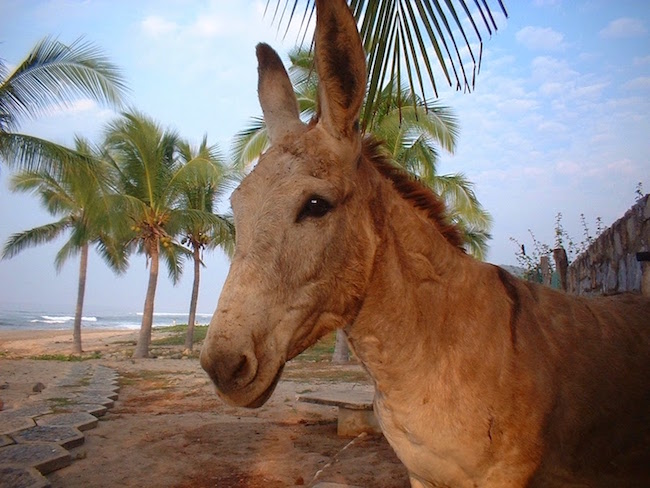
\includegraphics[keepaspectratio]{media/chapter_regression.jpg}}

\begin{quote}
The overall goal of any model is to provide a low-level description of
patterns within the data.
\end{quote}

\section{Lecture Materials}\label{lecture-materials-12}

\begin{quote}
\textbf{Lecture Slides:} Available interactively in the
\href{https://dyerlabteaching.github.io/Regression/slides.html\#/title-slide}{online
version}
\end{quote}

\begin{figure}[H]

{\centering \pandocbounded{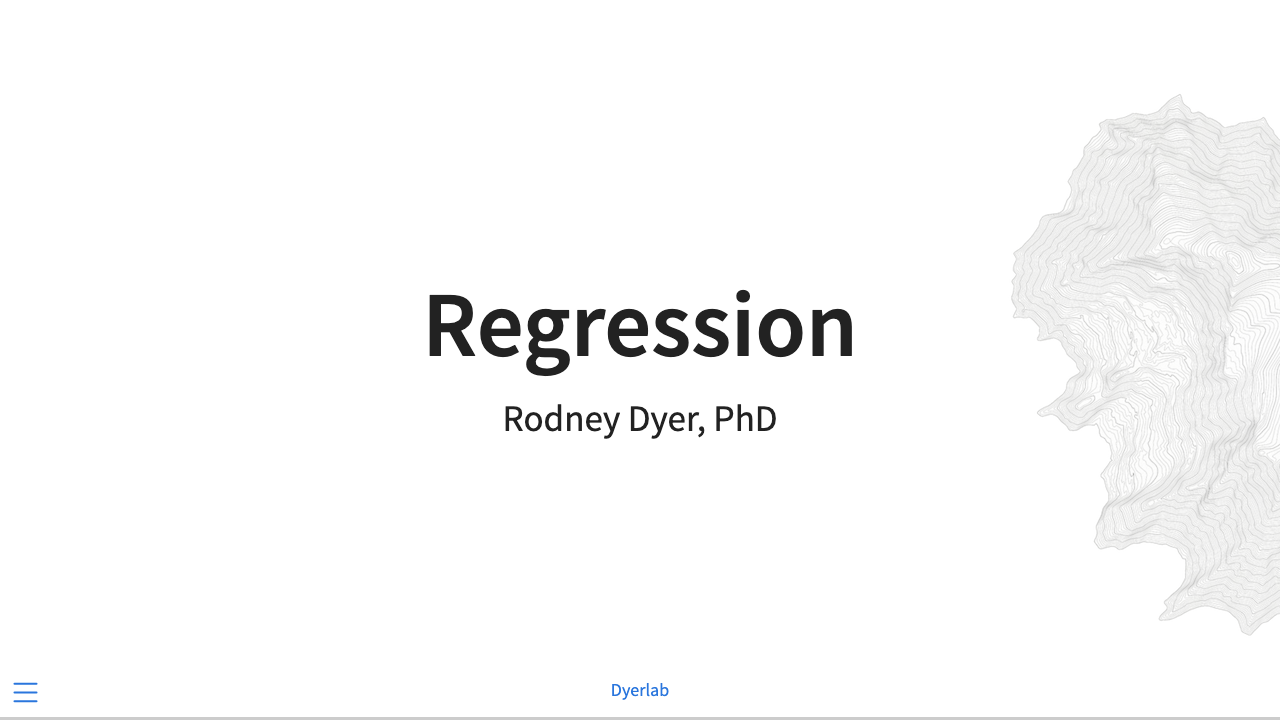
\includegraphics[keepaspectratio]{media/slides_regression.png}}

}

\caption{Lecture Slides}

\end{figure}%

If we think of all the variation in a data set, we can partition it into
the following components:

\[
\sigma_{Total}^2 = \sigma_{Model}^2 + \sigma_{Residual}^2
\]

In that some of the underlying variation goes towards explaining the
patterns in the data and the rest of the variation is \emph{residual}
(or left over). For regression analyses, consider the simple linear
regression model.

\[
y_{ij} = \beta_0 + \beta_1 x_{i} + \epsilon_j
\]

Where th terms \(\beta_0\) is the where the expected line interscepts
the y-axis when \(x = 0\), the coefficient \(\beta_1\) is the rate at
which the \(y\) (the results) changes \emph{per unit change} in \(x\)
(the predictor, and \(\epsilon\) is the left over variation (residual)
that each point has.

The null hypothesis for this kind of regression model is

\(H_O: \beta_1 = 0\)

We could have a hypothesis that \(\beta_0 = 0\) but that is often not
that interesting of an idea since that is a constant term in the
equation (n.b., we could subtract it out from both sides). If we have
more than one predictor variable, the null hypothesis becomes
\(H_O: \beta_i = 0; \forall i\) (that upside down triangle is `for
all').

Graphically, let us look at the following data as an example for basic
regression models.

\begin{Shaded}
\begin{Highlighting}[]
\NormalTok{df }\OtherTok{\textless{}{-}} \FunctionTok{data.frame}\NormalTok{( }\AttributeTok{x =} \DecValTok{1}\SpecialCharTok{:}\DecValTok{10}\NormalTok{,}
                  \AttributeTok{y =} \FunctionTok{c}\NormalTok{( }\FloatTok{15.5}\NormalTok{, }\FloatTok{28.1}\NormalTok{, }\FloatTok{22.3}\NormalTok{, }
                         \FloatTok{32.3}\NormalTok{, }\FloatTok{31.1}\NormalTok{, }\FloatTok{26.8}\NormalTok{, }
                         \FloatTok{41.8}\NormalTok{, }\FloatTok{30.3}\NormalTok{, }\FloatTok{47.9}\NormalTok{, }
                         \FloatTok{41.1}\NormalTok{) )}
\FunctionTok{ggplot}\NormalTok{( df, }\FunctionTok{aes}\NormalTok{(x,y) ) }\SpecialCharTok{+} 
  \FunctionTok{stat\_smooth}\NormalTok{( }\AttributeTok{method=}\StringTok{"lm"}\NormalTok{, }
               \AttributeTok{formula =}\NormalTok{ y }\SpecialCharTok{\textasciitilde{}}\NormalTok{ x, }
               \AttributeTok{se=}\ConstantTok{FALSE}\NormalTok{, }
               \AttributeTok{color=}\StringTok{"red"}\NormalTok{, }\AttributeTok{size=}\FloatTok{0.5}\NormalTok{) }\SpecialCharTok{+} 
  \FunctionTok{geom\_point}\NormalTok{() }
\end{Highlighting}
\end{Shaded}

\begin{verbatim}
Warning: Using `size` aesthetic for lines was deprecated in ggplot2 3.4.0.
i Please use `linewidth` instead.
\end{verbatim}

\pandocbounded{
\includegraphics[keepaspectratio]{narrative_regression_files/figure-pdf/unnamed-chunk-1-1.pdf}}

The notion here is to be estimate the underlying formula for that red
line that describes the variation in the original values in how
\texttt{y} changes systematically across measured values of \texttt{x}.

\section{Least Squares Fitting}\label{least-squares-fitting}

So how do we figure this out? One of the most common ways is to uses a
methods called \emph{Least Squared Distance} fitting. To describe this,
consider a set of hypothetical random models with random values
estimated for both the intercept (\(\beta_0\)) and slope (\(\beta_1\))
coefficients. These \emph{could be} close to a good models or not.

\begin{Shaded}
\begin{Highlighting}[]
\NormalTok{models }\OtherTok{\textless{}{-}} \FunctionTok{data.frame}\NormalTok{( }\AttributeTok{beta0 =} \FunctionTok{runif}\NormalTok{(}\DecValTok{250}\NormalTok{,}\SpecialCharTok{{-}}\DecValTok{20}\NormalTok{,}\DecValTok{40}\NormalTok{),}
                      \AttributeTok{beta1 =} \FunctionTok{runif}\NormalTok{(}\DecValTok{250}\NormalTok{, }\SpecialCharTok{{-}}\DecValTok{5}\NormalTok{, }\DecValTok{5}\NormalTok{))}
\FunctionTok{summary}\NormalTok{( models )}
\end{Highlighting}
\end{Shaded}

\begin{verbatim}
     beta0             beta1         
 Min.   :-19.917   Min.   :-4.97276  
 1st Qu.: -3.044   1st Qu.:-2.39615  
 Median : 12.105   Median :-0.09286  
 Mean   : 10.879   Mean   : 0.05048  
 3rd Qu.: 25.660   3rd Qu.: 2.78489  
 Max.   : 39.857   Max.   : 4.97483  
\end{verbatim}

We can plot these and the original data and all these randomly defined
models.

\begin{Shaded}
\begin{Highlighting}[]
\FunctionTok{ggplot}\NormalTok{() }\SpecialCharTok{+} 
  \FunctionTok{geom\_abline}\NormalTok{( }\FunctionTok{aes}\NormalTok{(}\AttributeTok{intercept =}\NormalTok{ beta0, }
                   \AttributeTok{slope =}\NormalTok{ beta1), }
               \AttributeTok{data =}\NormalTok{ models,}
               \AttributeTok{alpha =} \FloatTok{0.1}\NormalTok{) }\SpecialCharTok{+} 
  \FunctionTok{geom\_point}\NormalTok{( }\FunctionTok{aes}\NormalTok{(x,y), }
              \AttributeTok{data=}\NormalTok{df )}
\end{Highlighting}
\end{Shaded}

\pandocbounded{
\includegraphics[keepaspectratio]{narrative_regression_files/figure-pdf/unnamed-chunk-3-1.pdf}}

A least squares fit is one that minimizes the distances of each point
(in the y-axis) from the line created by the model. In the graph below,
we can see this would be the distances (squared so we do not have
positive and negative values) along the y-axis, between each point and
the fitted line.

The ``best model'' here is one that minimizes the sum of squared
distances distances.

\pandocbounded{
\includegraphics[keepaspectratio]{narrative_regression_files/figure-pdf/unnamed-chunk-4-1.pdf}}

Let's look at those hypothetical models. I'm going to make a few little
functions to help make the code look easy.

First, here is a function that returns the distances between the
original points and a hypothesized regression line defined by an
interscept and slope from the original points.

\begin{Shaded}
\begin{Highlighting}[]
\NormalTok{model\_distance }\OtherTok{\textless{}{-}} \ControlFlowTok{function}\NormalTok{( interscept, slope, X, Y ) \{}
\NormalTok{  yhat }\OtherTok{\textless{}{-}}\NormalTok{ interscept }\SpecialCharTok{+}\NormalTok{ slope }\SpecialCharTok{*}\NormalTok{ X}
\NormalTok{  diff }\OtherTok{\textless{}{-}}\NormalTok{ Y }\SpecialCharTok{{-}}\NormalTok{ yhat}
  \FunctionTok{return}\NormalTok{( }\FunctionTok{sqrt}\NormalTok{( }\FunctionTok{mean}\NormalTok{( diff }\SpecialCharTok{\^{}} \DecValTok{2}\NormalTok{ ) ) )}
\NormalTok{\}}
\end{Highlighting}
\end{Shaded}

Now, let's go through all the models and estimate the mean squared
distances between the proposed line (from intercept and slope) and the
original data.

\begin{Shaded}
\begin{Highlighting}[]
\NormalTok{models}\SpecialCharTok{$}\NormalTok{dist }\OtherTok{\textless{}{-}} \ConstantTok{NA}
\ControlFlowTok{for}\NormalTok{( i }\ControlFlowTok{in} \DecValTok{1}\SpecialCharTok{:}\FunctionTok{nrow}\NormalTok{(models) ) \{}
\NormalTok{  models}\SpecialCharTok{$}\NormalTok{dist[i] }\OtherTok{\textless{}{-}} \FunctionTok{model\_distance}\NormalTok{( models}\SpecialCharTok{$}\NormalTok{beta0[i],}
\NormalTok{                                    models}\SpecialCharTok{$}\NormalTok{beta1[i],}
\NormalTok{                                    df}\SpecialCharTok{$}\NormalTok{x,}
\NormalTok{                                    df}\SpecialCharTok{$}\NormalTok{y )}
\NormalTok{\}}
\FunctionTok{head}\NormalTok{( models )}
\end{Highlighting}
\end{Shaded}

\begin{verbatim}
      beta0       beta1      dist
1  33.80778  0.91037139 10.102587
2  13.63141  0.08394084 19.785239
3 -12.57540 -4.34637840 71.272487
4  14.90229  3.96385358  8.189733
5  26.33938  4.94398926 23.399586
6  19.39243  4.42672951 14.095856
\end{verbatim}

If we look through these models, we can see which are better than others
by sorting in increasing squared distance.

\begin{Shaded}
\begin{Highlighting}[]
\FunctionTok{ggplot}\NormalTok{()  }\SpecialCharTok{+} 
  \FunctionTok{geom\_abline}\NormalTok{( }\FunctionTok{aes}\NormalTok{(}\AttributeTok{intercept =}\NormalTok{ beta0,}
                   \AttributeTok{slope =}\NormalTok{ beta1, }
                   \AttributeTok{color =} \SpecialCharTok{{-}}\NormalTok{dist),}
               \AttributeTok{data =} \FunctionTok{filter}\NormalTok{( models, }\FunctionTok{rank}\NormalTok{(dist) }\SpecialCharTok{\textless{}=} \DecValTok{10}\NormalTok{ ),}
               \AttributeTok{alpha =} \FloatTok{0.5}\NormalTok{) }\SpecialCharTok{+} 
  \FunctionTok{geom\_point}\NormalTok{( }\FunctionTok{aes}\NormalTok{(x,y),}
              \AttributeTok{data=}\NormalTok{df) }
\end{Highlighting}
\end{Shaded}

\pandocbounded{
\includegraphics[keepaspectratio]{narrative_regression_files/figure-pdf/unnamed-chunk-7-1.pdf}}

These models in the \emph{parameter space} of intercepts and slopes can
be visualized as this. These red-circles are close to where the best
models are located.

\begin{Shaded}
\begin{Highlighting}[]
\FunctionTok{ggplot}\NormalTok{( models, }\FunctionTok{aes}\NormalTok{(}\AttributeTok{x =}\NormalTok{ beta0, }
                    \AttributeTok{y =}\NormalTok{ beta1,}
                    \AttributeTok{color =} \SpecialCharTok{{-}}\NormalTok{dist)) }\SpecialCharTok{+} 
  \FunctionTok{geom\_point}\NormalTok{( }\AttributeTok{data =} \FunctionTok{filter}\NormalTok{( models, }\FunctionTok{rank}\NormalTok{(dist) }\SpecialCharTok{\textless{}=} \DecValTok{10}\NormalTok{), }
              \AttributeTok{color =} \StringTok{"red"}\NormalTok{,}
              \AttributeTok{size =} \DecValTok{4}\NormalTok{) }\SpecialCharTok{+}
    \FunctionTok{geom\_point}\NormalTok{()}
\end{Highlighting}
\end{Shaded}

\pandocbounded{
\includegraphics[keepaspectratio]{narrative_regression_files/figure-pdf/unnamed-chunk-8-1.pdf}}

In addition to a random search, we can be a bit more systematic about it
and make a grid of interscept and slope values, using a \emph{grid
search}.

\begin{Shaded}
\begin{Highlighting}[]
\NormalTok{grid }\OtherTok{\textless{}{-}} \FunctionTok{expand.grid}\NormalTok{( }\AttributeTok{beta0 =} \FunctionTok{seq}\NormalTok{(}\DecValTok{15}\NormalTok{,}\DecValTok{20}\NormalTok{, }\AttributeTok{length =} \DecValTok{25}\NormalTok{),}
                     \AttributeTok{beta1 =} \FunctionTok{seq}\NormalTok{(}\DecValTok{2}\NormalTok{, }\FloatTok{3.5}\NormalTok{, }\AttributeTok{length =} \DecValTok{25}\NormalTok{))}
\NormalTok{grid}\SpecialCharTok{$}\NormalTok{dist }\OtherTok{\textless{}{-}} \ConstantTok{NA}
\ControlFlowTok{for}\NormalTok{( i }\ControlFlowTok{in} \DecValTok{1}\SpecialCharTok{:}\FunctionTok{nrow}\NormalTok{(grid) ) \{}
\NormalTok{  grid}\SpecialCharTok{$}\NormalTok{dist[i] }\OtherTok{\textless{}{-}} \FunctionTok{model\_distance}\NormalTok{( grid}\SpecialCharTok{$}\NormalTok{beta0[i],}
\NormalTok{                                  grid}\SpecialCharTok{$}\NormalTok{beta1[i],}
\NormalTok{                                  df}\SpecialCharTok{$}\NormalTok{x,}
\NormalTok{                                  df}\SpecialCharTok{$}\NormalTok{y )}
\NormalTok{\}}

\FunctionTok{ggplot}\NormalTok{( grid, }\FunctionTok{aes}\NormalTok{(}\AttributeTok{x =}\NormalTok{ beta0, }
                  \AttributeTok{y =}\NormalTok{ beta1,}
                  \AttributeTok{color =} \SpecialCharTok{{-}}\NormalTok{dist)) }\SpecialCharTok{+} 
  \FunctionTok{geom\_point}\NormalTok{( }\AttributeTok{data =} \FunctionTok{filter}\NormalTok{( grid, }\FunctionTok{rank}\NormalTok{(dist) }\SpecialCharTok{\textless{}=} \DecValTok{10}\NormalTok{), }
              \AttributeTok{color =} \StringTok{"red"}\NormalTok{,}
              \AttributeTok{size =} \DecValTok{4}\NormalTok{) }\SpecialCharTok{+}
  \FunctionTok{geom\_point}\NormalTok{()}
\end{Highlighting}
\end{Shaded}

\pandocbounded{
\includegraphics[keepaspectratio]{narrative_regression_files/figure-pdf/unnamed-chunk-9-1.pdf}}

You could imagine that we could iteratively soom in this grid and find
the best fit combination of \(\beta_0\) and \(\beta_1\) values until we
converged on a really well fit set.

There is a more direct way to get to these results (though is much less
pretty to look at) using the \texttt{lm()} linear models function.

\section{\texorpdfstring{Our Friend
\texttt{lm()}}{Our Friend lm()}}\label{our-friend-lm}

To specify a potential model, we need to get the function the form we
are interested in using.

\begin{Shaded}
\begin{Highlighting}[]
\NormalTok{fit }\OtherTok{\textless{}{-}} \FunctionTok{lm}\NormalTok{( y }\SpecialCharTok{\textasciitilde{}}\NormalTok{ x, }\AttributeTok{data =}\NormalTok{ df )}
\NormalTok{fit}
\end{Highlighting}
\end{Shaded}

\begin{verbatim}

Call:
lm(formula = y ~ x, data = df)

Coefficients:
(Intercept)            x  
     17.280        2.625  
\end{verbatim}

We can see that for the values of the coefficients (labeled
\emph{Interscept} and \emph{x}), it has a \texttt{model\_distance()} of

\begin{Shaded}
\begin{Highlighting}[]
\FunctionTok{model\_distance}\NormalTok{( }\SpecialCharTok{{-}}\FloatTok{1.76}\NormalTok{, }\FloatTok{3.385}\NormalTok{, df}\SpecialCharTok{$}\NormalTok{x, df}\SpecialCharTok{$}\NormalTok{y )}
\end{Highlighting}
\end{Shaded}

\begin{verbatim}
[1] 15.90948
\end{verbatim}

which we can see is pretty close in terms of the coefficients and has a
smaller model distance than those examined in the grid.

\begin{Shaded}
\begin{Highlighting}[]
\NormalTok{grid }\SpecialCharTok{\%\textgreater{}\%}
  \FunctionTok{arrange}\NormalTok{( dist ) }\SpecialCharTok{\%\textgreater{}\%}
  \FunctionTok{head}\NormalTok{( }\AttributeTok{n =} \DecValTok{1}\NormalTok{) }
\end{Highlighting}
\end{Shaded}

\begin{verbatim}
     beta0 beta1     dist
1 17.29167 2.625 5.240071
\end{verbatim}

Fortunately, we have a lot of additional information available to us
because we used the \texttt{lm()} function.

\section{Model Fit}\label{model-fit}

We can estimate a bunch of different models but before we look to see if
it well behaved. There are several interesting plots that we can examine
from the model object such as:

\begin{Shaded}
\begin{Highlighting}[]
\FunctionTok{plot}\NormalTok{( fit, }\AttributeTok{which =} \DecValTok{1}\NormalTok{ )}
\end{Highlighting}
\end{Shaded}

\pandocbounded{
\includegraphics[keepaspectratio]{narrative_regression_files/figure-pdf/unnamed-chunk-13-1.pdf}}

\begin{Shaded}
\begin{Highlighting}[]
\FunctionTok{plot}\NormalTok{( fit, }\AttributeTok{which =} \DecValTok{2}\NormalTok{ )}
\end{Highlighting}
\end{Shaded}

\pandocbounded{
\includegraphics[keepaspectratio]{narrative_regression_files/figure-pdf/unnamed-chunk-14-1.pdf}}

\begin{Shaded}
\begin{Highlighting}[]
\FunctionTok{plot}\NormalTok{( fit, }\AttributeTok{which =} \DecValTok{5}\NormalTok{ )}
\end{Highlighting}
\end{Shaded}

\pandocbounded{
\includegraphics[keepaspectratio]{narrative_regression_files/figure-pdf/unnamed-chunk-15-1.pdf}}

\section{Analysis of Variance Tables - Decomposing
Variation}\label{analysis-of-variance-tables---decomposing-variation}

Thus far, we've been able to estiamte a model, but is it one that
explains a significant amount of variation? To determine this, we use
the \emph{analysis of variance table}.

\begin{Shaded}
\begin{Highlighting}[]
\FunctionTok{anova}\NormalTok{( fit )}
\end{Highlighting}
\end{Shaded}

\begin{verbatim}
Analysis of Variance Table

Response: y
          Df Sum Sq Mean Sq F value   Pr(>F)   
x          1 568.67  568.67  16.568 0.003581 **
Residuals  8 274.58   34.32                    
---
Signif. codes:  0 '***' 0.001 '**' 0.01 '*' 0.05 '.' 0.1 ' ' 1
\end{verbatim}

The terms in this table are:

\begin{itemize}
\item
  Degrees of Freedom (\emph{df}): representing \texttt{1} degree of
  freedom for the model, and \texttt{N-1} for the residuals.
\item
  Sums of Squared Deviations:

  \begin{itemize}
  \tightlist
  \item
    \(SS_{Total} = \sum_{i=1}^N (y_i - \bar{y})^2\)
  \item
    \(SS_{Model} = \sum_{i=1}^N (\hat{y}_i - \bar{y})^2\), and
  \item
    \(SS_{Residual} = SS_{Total} - SS_{Model}\)
  \end{itemize}
\item
  Mean Squares (Standardization of the Sums of Squares for the degrees
  of freedom)

  \begin{itemize}
  \tightlist
  \item
    \(MS_{Model} = \frac{SS_{Model}}{df_{Model}}\)
  \item
    \(MS_{Residual} = \frac{SS_{Residual}}{df_{Residual}}\)
  \end{itemize}
\item
  The \(F\)-statistic is from a known distribution and is defined by the
  ratio of Mean Squared values.
\item
  \texttt{Pr(\textgreater{}F)} is the probability associated the value
  of the \(F\)-statistic and is dependent upon the degrees of freedom
  for the model and residuals.
\end{itemize}

\section{Variance Explained}\label{variance-explained}

There is a correlative measurement in regression models to the Pearson
Product Moment Coefficient, (\(\rho\)) in a statistic called \(R^2\).
This parameter tells you, \emph{How much of the observed variation in
\texttt{y} is explained by the model?}

The equation for \emph{R\^{}2} is:

\[
R^2 = \frac{SS_{Model}}{SS_{Total}}
\]

The value of this parameter is bound by 0 (the model explains no
variation) and 1.0 (the model explains all the variation in the data).
We can get to this and a few other parameters in the regression model by
taking its summary.

\begin{Shaded}
\begin{Highlighting}[]
\FunctionTok{summary}\NormalTok{( fit )}
\end{Highlighting}
\end{Shaded}

\begin{verbatim}

Call:
lm(formula = y ~ x, data = df)

Residuals:
    Min      1Q  Median      3Q     Max 
-7.9836 -4.0182 -0.8709  5.3064  6.9909 

Coefficients:
            Estimate Std. Error t value Pr(>|t|)   
(Intercept)   17.280      4.002   4.318  0.00255 **
x              2.626      0.645   4.070  0.00358 **
---
Signif. codes:  0 '***' 0.001 '**' 0.01 '*' 0.05 '.' 0.1 ' ' 1

Residual standard error: 5.859 on 8 degrees of freedom
Multiple R-squared:  0.6744,    Adjusted R-squared:  0.6337 
F-statistic: 16.57 on 1 and 8 DF,  p-value: 0.003581
\end{verbatim}

Just like the model itself, the \texttt{summary.lm} object also has all
these data contained within it in case you need to access them in
textual format or to annotate graphical output.

\begin{Shaded}
\begin{Highlighting}[]
\FunctionTok{names}\NormalTok{( }\FunctionTok{summary}\NormalTok{( fit ) )}
\end{Highlighting}
\end{Shaded}

\begin{verbatim}
 [1] "call"          "terms"         "residuals"     "coefficients" 
 [5] "aliased"       "sigma"         "df"            "r.squared"    
 [9] "adj.r.squared" "fstatistic"    "cov.unscaled" 
\end{verbatim}

Notice that the \texttt{p-value} is not in this list\ldots{} It is
estimable from the \texttt{fstatistic} and \texttt{df} values and here
is a quick function that returns the raw p-value by looking up the are
under the curve equal to or greater than the observed
\texttt{fstatistic} with those degrees of freedom.

\begin{Shaded}
\begin{Highlighting}[]
\NormalTok{get\_pval }\OtherTok{\textless{}{-}} \ControlFlowTok{function}\NormalTok{( model ) \{}
\NormalTok{  f }\OtherTok{\textless{}{-}} \FunctionTok{summary}\NormalTok{( model )}\SpecialCharTok{$}\NormalTok{fstatistic[}\DecValTok{1}\NormalTok{]}
\NormalTok{  df1 }\OtherTok{\textless{}{-}} \FunctionTok{summary}\NormalTok{( model )}\SpecialCharTok{$}\NormalTok{fstatistic[}\DecValTok{2}\NormalTok{]}
\NormalTok{  df2 }\OtherTok{\textless{}{-}} \FunctionTok{summary}\NormalTok{( model )}\SpecialCharTok{$}\NormalTok{fstatistic[}\DecValTok{3}\NormalTok{]}
\NormalTok{  p }\OtherTok{\textless{}{-}} \FunctionTok{as.numeric}\NormalTok{( }\FloatTok{1.0} \SpecialCharTok{{-}} \FunctionTok{pf}\NormalTok{( f, df1, df2 ) )}
  \FunctionTok{return}\NormalTok{( p  )}
\NormalTok{\}}

\FunctionTok{get\_pval}\NormalTok{( fit )}
\end{Highlighting}
\end{Shaded}

\begin{verbatim}
[1] 0.0035813
\end{verbatim}

As an often-overlooked side effect, the \(R^2\) from a simple one
predictor regression model and the correlation coefficient \(r\) from
\texttt{cor.test(method=\textquotesingle{}pearson\textquotesingle{})}
are related as follows:

\begin{Shaded}
\begin{Highlighting}[]
\FunctionTok{c}\NormalTok{( }\StringTok{\textasciigrave{}}\AttributeTok{Regression R\^{}2}\StringTok{\textasciigrave{}} \OtherTok{=} \FunctionTok{summary}\NormalTok{( fit )}\SpecialCharTok{$}\NormalTok{r.squared,}
   \StringTok{\textasciigrave{}}\AttributeTok{Squared Correlation}\StringTok{\textasciigrave{}} \OtherTok{=} \FunctionTok{as.numeric}\NormalTok{( }\FunctionTok{cor.test}\NormalTok{( df}\SpecialCharTok{$}\NormalTok{x, df}\SpecialCharTok{$}\NormalTok{y )}\SpecialCharTok{$}\NormalTok{estimate}\SpecialCharTok{\^{}}\DecValTok{2}\NormalTok{ ) )}
\end{Highlighting}
\end{Shaded}

\begin{verbatim}
     Regression R^2 Squared Correlation 
          0.6743782           0.6743782 
\end{verbatim}

(e.g., the square of the correlation estimate \(r\) is equal to
\(R^2\)).

\section{Extensions of the Model}\label{extensions-of-the-model}

There are several helper functions for dealing with regression models
such as finding the predicted values.

\begin{Shaded}
\begin{Highlighting}[]
\FunctionTok{predict}\NormalTok{( fit ) }\OtherTok{{-}\textgreater{}}\NormalTok{ yhat }
\NormalTok{yhat }
\end{Highlighting}
\end{Shaded}

\begin{verbatim}
       1        2        3        4        5        6        7        8 
19.90545 22.53091 25.15636 27.78182 30.40727 33.03273 35.65818 38.28364 
       9       10 
40.90909 43.53455 
\end{verbatim}

And we can plot it as:

\begin{Shaded}
\begin{Highlighting}[]
\FunctionTok{plot}\NormalTok{( yhat }\SpecialCharTok{\textasciitilde{}}\NormalTok{ df}\SpecialCharTok{$}\NormalTok{x, }\AttributeTok{type=}\StringTok{\textquotesingle{}l\textquotesingle{}}\NormalTok{, }\AttributeTok{bty=}\StringTok{"n"}\NormalTok{, }\AttributeTok{col=}\StringTok{"red"}\NormalTok{ )}
\end{Highlighting}
\end{Shaded}

\pandocbounded{
\includegraphics[keepaspectratio]{narrative_regression_files/figure-pdf/unnamed-chunk-22-1.pdf}}

The residual values (e.g., the distance between the original data on the
y-axis and the fitted regression model).

\begin{Shaded}
\begin{Highlighting}[]
\FunctionTok{residuals}\NormalTok{( fit ) }\OtherTok{{-}\textgreater{}}\NormalTok{ resids}
\NormalTok{resids }
\end{Highlighting}
\end{Shaded}

\begin{verbatim}
         1          2          3          4          5          6          7 
-4.4054545  5.5690909 -2.8563636  4.5181818  0.6927273 -6.2327273  6.1418182 
         8          9         10 
-7.9836364  6.9909091 -2.4345455 
\end{verbatim}

We almost \textbf{always} need to look at the residuals of a regression
model to help diagnose any potential problems (as shown above in the
plots of the raw model itself).

\begin{Shaded}
\begin{Highlighting}[]
\FunctionTok{plot}\NormalTok{( resids }\SpecialCharTok{\textasciitilde{}}\NormalTok{ yhat, }\AttributeTok{bty=}\StringTok{"n"}\NormalTok{, }\AttributeTok{xlab=}\StringTok{"Predicted Values"}\NormalTok{, }\AttributeTok{ylab=}\StringTok{"Residuals (yhat {-} y)"}\NormalTok{, }\AttributeTok{pch=}\DecValTok{16}\NormalTok{ )}
\FunctionTok{abline}\NormalTok{(}\DecValTok{0}\NormalTok{, }\DecValTok{0}\NormalTok{, }\AttributeTok{lty=}\DecValTok{2}\NormalTok{, }\AttributeTok{col=}\StringTok{"red"}\NormalTok{)}
\end{Highlighting}
\end{Shaded}

\pandocbounded{
\includegraphics[keepaspectratio]{narrative_regression_files/figure-pdf/unnamed-chunk-24-1.pdf}}

\section{Comparing Models}\label{comparing-models}

OK, so we have a model that appears to suggest that the predicted values
in \texttt{x} can explain the variation observed in \texttt{y}. Great.
But, is this the best model or only one that is sufficiently \emph{meh}
such that we can reject the null hypothesis. How can we tell?

There are two parameters that we have already looked at that may help.
These are:

\begin{itemize}
\item
  The \texttt{P-value}: Models with smaller probabilities could be
  considered more informative.
\item
  The \(R^2\): Models that explain more of the variation may be
  considered more informative.
\end{itemize}

Let's start by looking at some airquality data we have played with
previously when working on
\href{https://dyerlab.github.io/ENVS-Lectures/r_language/data_frames/homework.nb.html}{data.frame
objects}.

\begin{Shaded}
\begin{Highlighting}[]
\NormalTok{airquality }\SpecialCharTok{\%\textgreater{}\%}
  \FunctionTok{select}\NormalTok{( }\SpecialCharTok{{-}}\NormalTok{Month, }\SpecialCharTok{{-}}\NormalTok{Day ) }\OtherTok{{-}\textgreater{}}\NormalTok{ df.air}
\FunctionTok{summary}\NormalTok{( df.air )}
\end{Highlighting}
\end{Shaded}

\begin{verbatim}
     Ozone           Solar.R           Wind             Temp      
 Min.   :  1.00   Min.   :  7.0   Min.   : 1.700   Min.   :56.00  
 1st Qu.: 18.00   1st Qu.:115.8   1st Qu.: 7.400   1st Qu.:72.00  
 Median : 31.50   Median :205.0   Median : 9.700   Median :79.00  
 Mean   : 42.13   Mean   :185.9   Mean   : 9.958   Mean   :77.88  
 3rd Qu.: 63.25   3rd Qu.:258.8   3rd Qu.:11.500   3rd Qu.:85.00  
 Max.   :168.00   Max.   :334.0   Max.   :20.700   Max.   :97.00  
 NA's   :37       NA's   :7                                       
\end{verbatim}

Let's assume that we are interested in trying to explain the variation
in \texttt{Ozone} (the response) by one or more of the other variables
as predictors.

\begin{Shaded}
\begin{Highlighting}[]
\NormalTok{fit.solar }\OtherTok{\textless{}{-}} \FunctionTok{lm}\NormalTok{( Ozone }\SpecialCharTok{\textasciitilde{}}\NormalTok{ Solar.R, }\AttributeTok{data =}\NormalTok{ df.air )}
\FunctionTok{anova}\NormalTok{( fit.solar )}
\end{Highlighting}
\end{Shaded}

\begin{verbatim}
Analysis of Variance Table

Response: Ozone
           Df Sum Sq Mean Sq F value    Pr(>F)    
Solar.R     1  14780 14779.7  15.053 0.0001793 ***
Residuals 109 107022   981.9                      
---
Signif. codes:  0 '***' 0.001 '**' 0.01 '*' 0.05 '.' 0.1 ' ' 1
\end{verbatim}

Let's look at all the predictors and take a look at both the
\texttt{p-value} and \texttt{R-squared}.

\begin{Shaded}
\begin{Highlighting}[]
\NormalTok{fit.temp }\OtherTok{\textless{}{-}} \FunctionTok{lm}\NormalTok{( Ozone }\SpecialCharTok{\textasciitilde{}}\NormalTok{ Temp, }\AttributeTok{data =}\NormalTok{ df.air )}
\NormalTok{fit.wind }\OtherTok{\textless{}{-}} \FunctionTok{lm}\NormalTok{( Ozone }\SpecialCharTok{\textasciitilde{}}\NormalTok{ Wind, }\AttributeTok{data =}\NormalTok{ df.air )}

\FunctionTok{data.frame}\NormalTok{( }\AttributeTok{Model =} \FunctionTok{c}\NormalTok{( }\StringTok{"Ozone \textasciitilde{} Solar"}\NormalTok{,}
                       \StringTok{"Ozone \textasciitilde{} Temp"}\NormalTok{,}
                       \StringTok{"Ozone \textasciitilde{} Wind"}\NormalTok{), }
            \AttributeTok{R2 =} \FunctionTok{c}\NormalTok{( }\FunctionTok{summary}\NormalTok{( fit.solar )}\SpecialCharTok{$}\NormalTok{r.squared,}
                    \FunctionTok{summary}\NormalTok{( fit.temp )}\SpecialCharTok{$}\NormalTok{r.squared,}
                    \FunctionTok{summary}\NormalTok{( fit.wind )}\SpecialCharTok{$}\NormalTok{r.squared ), }
            \AttributeTok{P =} \FunctionTok{c}\NormalTok{( }\FunctionTok{get\_pval}\NormalTok{( fit.solar), }
                   \FunctionTok{get\_pval}\NormalTok{( fit.temp ),}
                   \FunctionTok{get\_pval}\NormalTok{( fit.wind ) ) ) }\OtherTok{{-}\textgreater{}}\NormalTok{ df.models}

\NormalTok{df.models }\SpecialCharTok{\%\textgreater{}\%}
  \FunctionTok{arrange}\NormalTok{( }\SpecialCharTok{{-}}\NormalTok{R2 ) }\SpecialCharTok{\%\textgreater{}\%}
  \FunctionTok{mutate}\NormalTok{( }\AttributeTok{P =} \FunctionTok{format}\NormalTok{( P, }\AttributeTok{scientific=}\ConstantTok{TRUE}\NormalTok{, }\AttributeTok{digits=}\DecValTok{3}\NormalTok{)) }\SpecialCharTok{\%\textgreater{}\%}
  \FunctionTok{kable}\NormalTok{( }\AttributeTok{caption =} \StringTok{"Model parameters predicting mean ozone in parts per billion mresured in New York during the period of 1 May 2973 {-} 30 September 2973."}\NormalTok{,}
         \AttributeTok{digits =} \DecValTok{3}\NormalTok{) }\SpecialCharTok{\%\textgreater{}\%}
  \FunctionTok{kable\_minimal}\NormalTok{()}
\end{Highlighting}
\end{Shaded}

\begin{longtable}[t]{lrl}
\caption{\label{tab:unnamed-chunk-27}Model parameters predicting mean ozone in parts per billion mresured in New York during the period of 1 May 2973 - 30 September 2973.}\\
\toprule
Model & R2 & P\\
\midrule
Ozone \textasciitilde{} Temp & 0.488 & 0.00e+00\\
Ozone \textasciitilde{} Wind & 0.362 & 9.27e-13\\
Ozone \textasciitilde{} Solar & 0.121 & 1.79e-04\\
\bottomrule
\end{longtable}

So if we look at these results, we see that in both \(R^2\) and \(P\),
the model with \texttt{Temp} seems to be most explanatory as well as
having the lowest probability. But is is significantly better?

How about if we start adding more than one variable to the equation so
that we now have two variables (multiple regression) with the general
model specified as:

\[
y = \beta_0 + \beta_1 x_1 + beta_2 x_2 + \epsilon
\]

Now, we are estimating two regression coefficients and an interscept.
For three predictors, this gives us 3 more models.

\begin{Shaded}
\begin{Highlighting}[]
\NormalTok{fit.temp.wind }\OtherTok{\textless{}{-}} \FunctionTok{lm}\NormalTok{( Ozone }\SpecialCharTok{\textasciitilde{}}\NormalTok{ Temp }\SpecialCharTok{+}\NormalTok{ Wind, }\AttributeTok{data =}\NormalTok{ df.air )}
\NormalTok{fit.temp.solar }\OtherTok{\textless{}{-}} \FunctionTok{lm}\NormalTok{( Ozone }\SpecialCharTok{\textasciitilde{}}\NormalTok{ Temp }\SpecialCharTok{+}\NormalTok{ Solar.R, }\AttributeTok{data =}\NormalTok{ df.air )}
\NormalTok{fit.wind.solar }\OtherTok{\textless{}{-}} \FunctionTok{lm}\NormalTok{( Ozone }\SpecialCharTok{\textasciitilde{}}\NormalTok{ Wind }\SpecialCharTok{+}\NormalTok{ Solar.R, }\AttributeTok{data =}\NormalTok{ df.air )}
\end{Highlighting}
\end{Shaded}

Now, we can add these output to the table.

\begin{Shaded}
\begin{Highlighting}[]
\NormalTok{df.models }\OtherTok{\textless{}{-}} \FunctionTok{rbind}\NormalTok{( df.models, }
                    \FunctionTok{data.frame}\NormalTok{( }\AttributeTok{Model =} \FunctionTok{c}\NormalTok{( }\StringTok{"Ozone \textasciitilde{} Temp + Wind"}\NormalTok{,}
                                           \StringTok{"Ozone \textasciitilde{} Temp + Solar"}\NormalTok{,}
                                           \StringTok{"Ozone \textasciitilde{} Wind + Solar"}\NormalTok{ ),}
                                \AttributeTok{R2 =} \FunctionTok{c}\NormalTok{( }\FunctionTok{summary}\NormalTok{( fit.temp.wind )}\SpecialCharTok{$}\NormalTok{r.squared,}
                                        \FunctionTok{summary}\NormalTok{( fit.temp.solar )}\SpecialCharTok{$}\NormalTok{r.squared,}
                                        \FunctionTok{summary}\NormalTok{( fit.wind.solar )}\SpecialCharTok{$}\NormalTok{r.squared ),}
                                \AttributeTok{P =} \FunctionTok{c}\NormalTok{( }\FunctionTok{get\_pval}\NormalTok{( fit.temp.wind),}
                                       \FunctionTok{get\_pval}\NormalTok{( fit.temp.solar),}
                                       \FunctionTok{get\_pval}\NormalTok{( fit.wind.solar) )}
\NormalTok{                                ))}
\NormalTok{df.models }\SpecialCharTok{\%\textgreater{}\%}
  \FunctionTok{mutate}\NormalTok{( }\AttributeTok{P =} \FunctionTok{format}\NormalTok{( P, }\AttributeTok{scientific=}\ConstantTok{TRUE}\NormalTok{, }\AttributeTok{digits=}\DecValTok{3}\NormalTok{)) }\SpecialCharTok{\%\textgreater{}\%}
  \FunctionTok{kable}\NormalTok{( }\AttributeTok{caption =} \StringTok{"Model parameters predicting mean ozone in parts per billion mresured in New York during the period of 1 May 2973 {-} 30 September 2973."}\NormalTok{,}
         \AttributeTok{digits =} \DecValTok{3}\NormalTok{) }\SpecialCharTok{\%\textgreater{}\%}
  \FunctionTok{kable\_minimal}\NormalTok{()}
\end{Highlighting}
\end{Shaded}

\begin{longtable}[t]{lrl}
\caption{\label{tab:unnamed-chunk-29}Model parameters predicting mean ozone in parts per billion mresured in New York during the period of 1 May 2973 - 30 September 2973.}\\
\toprule
Model & R2 & P\\
\midrule
Ozone \textasciitilde{} Solar & 0.121 & 1.79e-04\\
Ozone \textasciitilde{} Temp & 0.488 & 0.00e+00\\
Ozone \textasciitilde{} Wind & 0.362 & 9.27e-13\\
Ozone \textasciitilde{} Temp + Wind & 0.569 & 0.00e+00\\
Ozone \textasciitilde{} Temp + Solar & 0.510 & 0.00e+00\\
\addlinespace
Ozone \textasciitilde{} Wind + Solar & 0.449 & 9.99e-15\\
\bottomrule
\end{longtable}

Hmmmmmm.

And for completeness, let's just add the model that has all three
predictors

\[
y = \beta_0 + \beta_1 x_1 + \beta_2 x_2 + \beta_3 x_3 + \epsilon
\]

\begin{Shaded}
\begin{Highlighting}[]
\NormalTok{fit.all }\OtherTok{\textless{}{-}} \FunctionTok{lm}\NormalTok{( Ozone }\SpecialCharTok{\textasciitilde{}}\NormalTok{ Solar.R }\SpecialCharTok{+}\NormalTok{ Temp }\SpecialCharTok{+}\NormalTok{ Wind, }\AttributeTok{data =}\NormalTok{ df.air )}
\end{Highlighting}
\end{Shaded}

Now let's add that one

\begin{Shaded}
\begin{Highlighting}[]
\NormalTok{df.models }\OtherTok{\textless{}{-}} \FunctionTok{rbind}\NormalTok{( df.models, }
                    \FunctionTok{data.frame}\NormalTok{( }\AttributeTok{Model =} \FunctionTok{c}\NormalTok{( }\StringTok{"Ozone \textasciitilde{} Temp + Wind + Solar"}\NormalTok{),}
                                \AttributeTok{R2 =} \FunctionTok{c}\NormalTok{( }\FunctionTok{summary}\NormalTok{( fit.all )}\SpecialCharTok{$}\NormalTok{r.squared ),}
                                \AttributeTok{P =} \FunctionTok{c}\NormalTok{( }\FunctionTok{get\_pval}\NormalTok{( fit.all)  )}
\NormalTok{                                ))}


\NormalTok{df.models}\SpecialCharTok{$}\NormalTok{P }\OtherTok{=} \FunctionTok{cell\_spec}\NormalTok{( }\FunctionTok{format}\NormalTok{( df.models}\SpecialCharTok{$}\NormalTok{P, }
                                 \AttributeTok{digits=}\DecValTok{3}\NormalTok{, }
                                 \AttributeTok{scientific=}\ConstantTok{TRUE}\NormalTok{), }
                         \AttributeTok{color =} \FunctionTok{ifelse}\NormalTok{( df.models}\SpecialCharTok{$}\NormalTok{P }\SpecialCharTok{==} \FunctionTok{min}\NormalTok{(df.models}\SpecialCharTok{$}\NormalTok{P), }
                                         \StringTok{"red"}\NormalTok{,}
                                         \StringTok{"black"}\NormalTok{))}
\NormalTok{df.models}\SpecialCharTok{$}\NormalTok{R2 }\OtherTok{=} \FunctionTok{cell\_spec}\NormalTok{( }\FunctionTok{format}\NormalTok{( df.models}\SpecialCharTok{$}\NormalTok{R2, }
                                  \AttributeTok{digits=}\DecValTok{3}\NormalTok{, }
                                  \AttributeTok{scientific=}\ConstantTok{TRUE}\NormalTok{), }
                          \AttributeTok{color =} \FunctionTok{ifelse}\NormalTok{( df.models}\SpecialCharTok{$}\NormalTok{R2 }\SpecialCharTok{==} \FunctionTok{max}\NormalTok{( df.models}\SpecialCharTok{$}\NormalTok{R2), }
                                          \StringTok{"green"}\NormalTok{,}
                                          \StringTok{"black"}\NormalTok{))}

\NormalTok{df.models }\SpecialCharTok{\%\textgreater{}\%}
  \FunctionTok{mutate}\NormalTok{( }\AttributeTok{P =} \FunctionTok{format}\NormalTok{( P, }\AttributeTok{digits=}\DecValTok{3}\NormalTok{, }\AttributeTok{scientific =} \ConstantTok{TRUE}\NormalTok{) ) }\SpecialCharTok{\%\textgreater{}\%} 
  \FunctionTok{kable}\NormalTok{( }\AttributeTok{caption =} \StringTok{"Model parameters predicting mean ozone in parts per billion mresured in New York during the period of 1 May 2973 {-} 30 September 2973.  Values in green indicate the model with the largest variance explained and those in red indicate models with the lowest probability."}\NormalTok{,}
         \AttributeTok{escape =} \ConstantTok{FALSE}\NormalTok{) }\SpecialCharTok{\%\textgreater{}\%}
  \FunctionTok{kable\_paper}\NormalTok{( }\StringTok{"striped"}\NormalTok{, }\AttributeTok{full\_width =} \ConstantTok{FALSE}\NormalTok{ )}
\end{Highlighting}
\end{Shaded}

\begin{longtable}[t]{lll}
\caption{\label{tab:unnamed-chunk-31}Model parameters predicting mean ozone in parts per billion mresured in New York during the period of 1 May 2973 - 30 September 2973.  Values in green indicate the model with the largest variance explained and those in red indicate models with the lowest probability.}\\
\toprule
Model & R2 & P\\
\midrule
Ozone \textasciitilde{} Solar & \textbackslash{}textcolor\{black\}\{1.21e-01\} & \textbackslash{}textcolor\{black\}\{1.79e-04\}\\
Ozone \textasciitilde{} Temp & \textbackslash{}textcolor\{black\}\{4.88e-01\} & \textbackslash{}textcolor\{red\}\{0.00e+00\}\\
Ozone \textasciitilde{} Wind & \textbackslash{}textcolor\{black\}\{3.62e-01\} & \textbackslash{}textcolor\{black\}\{9.27e-13\}\\
Ozone \textasciitilde{} Temp + Wind & \textbackslash{}textcolor\{black\}\{5.69e-01\} & \textbackslash{}textcolor\{red\}\{0.00e+00\}\\
Ozone \textasciitilde{} Temp + Solar & \textbackslash{}textcolor\{black\}\{5.10e-01\} & \textbackslash{}textcolor\{red\}\{0.00e+00\}\\
\addlinespace
Ozone \textasciitilde{} Wind + Solar & \textbackslash{}textcolor\{black\}\{4.49e-01\} & \textbackslash{}textcolor\{black\}\{9.99e-15\}\\
Ozone \textasciitilde{} Temp + Wind + Solar & \textbackslash{}textcolor\{green\}\{6.06e-01\} & \textbackslash{}textcolor\{red\}\{0.00e+00\}\\
\bottomrule
\end{longtable}

So how do we figure out which one is best?

\subsection{Effects of Adding
Parameters}\label{effects-of-adding-parameters}

Before we can answer this, we should be clear about one thing. We are
getting more variance explained by adding more predictor variables. In
fact, by adding any variable, whether they are informative or not, one
can explain some amount of the Sums of Squares in a model. Taken to the
extreme, this means that we could add an infinite number of explanatory
variables to a model and explain all the variation there is!

Here is an example using our small data set. I'm going to make several
models, one of which is the original one and the remaining add one more
predeictor varible that is made up of a random variables. We will then
look at the \(R^2\) of each of these models.

\begin{Shaded}
\begin{Highlighting}[]
\NormalTok{random.models  }\OtherTok{\textless{}{-}} \FunctionTok{list}\NormalTok{()}
\NormalTok{random.models[[}\StringTok{"Ozone \textasciitilde{} Temp"}\NormalTok{]] }\OtherTok{\textless{}{-}}\NormalTok{ fit.temp}
\NormalTok{random.models[[}\StringTok{"Ozone \textasciitilde{} Wind"}\NormalTok{]] }\OtherTok{\textless{}{-}}\NormalTok{ fit.wind}
\NormalTok{random.models[[}\StringTok{"Ozone \textasciitilde{} Solar"}\NormalTok{]] }\OtherTok{\textless{}{-}}\NormalTok{ fit.solar}
\NormalTok{random.models[[}\StringTok{"Ozone \textasciitilde{} Temp + Wind"}\NormalTok{]] }\OtherTok{\textless{}{-}}\NormalTok{ fit.temp.wind}
\NormalTok{random.models[[}\StringTok{"Ozone \textasciitilde{} Temp + Solar"}\NormalTok{]] }\OtherTok{\textless{}{-}}\NormalTok{ fit.temp.solar}
\NormalTok{random.models[[}\StringTok{"Ozone \textasciitilde{} Wind + Solar"}\NormalTok{]] }\OtherTok{\textless{}{-}}\NormalTok{ fit.wind.solar}
\NormalTok{random.models[[ }\StringTok{"Ozone \textasciitilde{} Temp + Wind + Solar"}\NormalTok{ ]] }\OtherTok{\textless{}{-}}\NormalTok{ fit.all}

\NormalTok{df.tmp }\OtherTok{\textless{}{-}}\NormalTok{ df.air}

\ControlFlowTok{for}\NormalTok{( i }\ControlFlowTok{in} \DecValTok{1}\SpecialCharTok{:}\DecValTok{8}\NormalTok{ ) \{}
\NormalTok{  lbl }\OtherTok{\textless{}{-}} \FunctionTok{paste}\NormalTok{(}\StringTok{"Ozone \textasciitilde{} Temp + Wind + Solar + "}\NormalTok{, i, }\StringTok{" Random Variables"}\NormalTok{, }\AttributeTok{sep=}\StringTok{""}\NormalTok{)}
\NormalTok{  df.tmp[[lbl]] }\OtherTok{\textless{}{-}} \FunctionTok{rnorm}\NormalTok{( }\FunctionTok{nrow}\NormalTok{(df.tmp) )}
\NormalTok{  random.models[[lbl]] }\OtherTok{\textless{}{-}} \FunctionTok{lm}\NormalTok{( Ozone }\SpecialCharTok{\textasciitilde{}}\NormalTok{ ., }\AttributeTok{data =}\NormalTok{ df.tmp ) }
\NormalTok{\}}

\FunctionTok{data.frame}\NormalTok{( }\AttributeTok{Models =} \FunctionTok{names}\NormalTok{( random.models ),}
            \AttributeTok{R2 =} \FunctionTok{sapply}\NormalTok{( random.models, }
                          \AttributeTok{FUN =} \ControlFlowTok{function}\NormalTok{( x ) }\FunctionTok{return}\NormalTok{( }\FunctionTok{summary}\NormalTok{( x )}\SpecialCharTok{$}\NormalTok{r.squared), }
                          \AttributeTok{simplify =} \ConstantTok{TRUE}\NormalTok{ ),}
            \AttributeTok{P =} \FunctionTok{sapply}\NormalTok{( random.models, }
                        \AttributeTok{FUN =}\NormalTok{ get\_pval ) ) }\OtherTok{{-}\textgreater{}}\NormalTok{ df.random}

\NormalTok{df.random }\SpecialCharTok{\%\textgreater{}\%}
  \FunctionTok{kable}\NormalTok{( }\AttributeTok{caption =} \StringTok{"Fraction of variation explained by original variable as well as models with incrementally more predictor variables made up of randomly derived data."}\NormalTok{,}
         \AttributeTok{digits=}\DecValTok{4}\NormalTok{,}
         \AttributeTok{row.names =} \ConstantTok{FALSE}\NormalTok{ ) }\SpecialCharTok{\%\textgreater{}\%}
  \FunctionTok{kable\_paper}\NormalTok{(}\StringTok{"striped"}\NormalTok{, }\AttributeTok{full\_width =} \ConstantTok{FALSE}\NormalTok{ )}
\end{Highlighting}
\end{Shaded}

\begin{longtable}[t]{lrr}
\caption{\label{tab:unnamed-chunk-32}Fraction of variation explained by original variable as well as models with incrementally more predictor variables made up of randomly derived data.}\\
\toprule
Models & R2 & P\\
\midrule
Ozone \textasciitilde{} Temp & 0.4877 & 0e+00\\
Ozone \textasciitilde{} Wind & 0.3619 & 0e+00\\
Ozone \textasciitilde{} Solar & 0.1213 & 2e-04\\
Ozone \textasciitilde{} Temp + Wind & 0.5687 & 0e+00\\
Ozone \textasciitilde{} Temp + Solar & 0.5103 & 0e+00\\
\addlinespace
Ozone \textasciitilde{} Wind + Solar & 0.4495 & 0e+00\\
Ozone \textasciitilde{} Temp + Wind + Solar & 0.6059 & 0e+00\\
Ozone \textasciitilde{} Temp + Wind + Solar + 1 Random Variables & 0.6072 & 0e+00\\
Ozone \textasciitilde{} Temp + Wind + Solar + 2 Random Variables & 0.6184 & 0e+00\\
Ozone \textasciitilde{} Temp + Wind + Solar + 3 Random Variables & 0.6187 & 0e+00\\
\addlinespace
Ozone \textasciitilde{} Temp + Wind + Solar + 4 Random Variables & 0.6200 & 0e+00\\
Ozone \textasciitilde{} Temp + Wind + Solar + 5 Random Variables & 0.6201 & 0e+00\\
Ozone \textasciitilde{} Temp + Wind + Solar + 6 Random Variables & 0.6237 & 0e+00\\
Ozone \textasciitilde{} Temp + Wind + Solar + 7 Random Variables & 0.6261 & 0e+00\\
Ozone \textasciitilde{} Temp + Wind + Solar + 8 Random Variables & 0.6270 & 0e+00\\
\bottomrule
\end{longtable}

So if we just add random data to a model, we get a better fit!!!! Sounds
great. That is easy! I can \textbf{always} get the best fit there is!

This is a well-known situation in statistics. An in fact, we must be
very careful when we are examining the differences between models and
attempting to decide which set of models are actually better than other
sets of models.

\section{Model Fitting}\label{model-fitting}

To get around this, we have a few tools at our disposal. The most common
approach is to look at the \emph{information content} in each model
relative to the amount of pedictor variables. In essence, we must
\emph{punish} ourselves for adding more predictors so that we do not all
run around and add random data to our models. The most common one is
called Akaike Information Criterion (AIC), and provide a general
framework for comparing several models.

\[
AIC = -2 \ln L + 2p
\]

Where \(L\) is the log likelihood estimate of the variance and \(p\) is
the number of parameters. What this does is allow you to evaluate
different models with different subsets of parameters. In general, the
best model is the one with the smallest value for \texttt{AIC}.

We can also evaluate the relative values of all the models by looking in
the difference between the ``best'' model and the rest by taking the
difference

\[
\delta AIC = AIC - min(AIC)
\]

The prevailing notion is that models that have \(\delta AIC < 2.0\)
should be considered as almost equally informative, where as those whose
\(\delta AIC > 5.0\) are to be rejected as being informative. That
\(2.0 \le \delta AIC \le 5.0\) range is where it gets a bit fuzzy.

\begin{Shaded}
\begin{Highlighting}[]
\NormalTok{df.random}\SpecialCharTok{$}\NormalTok{AIC }\OtherTok{\textless{}{-}} \FunctionTok{sapply}\NormalTok{( random.models, }
                         \AttributeTok{FUN =}\NormalTok{ AIC, }
                         \AttributeTok{simplify =} \ConstantTok{TRUE}\NormalTok{ )}

\NormalTok{df.random}\SpecialCharTok{$}\NormalTok{deltaAIC }\OtherTok{=}\NormalTok{ df.random}\SpecialCharTok{$}\NormalTok{AIC }\SpecialCharTok{{-}} \FunctionTok{min}\NormalTok{( df.random}\SpecialCharTok{$}\NormalTok{A)}

\NormalTok{df.random }\SpecialCharTok{\%\textgreater{}\%}
  \FunctionTok{select}\NormalTok{( }\SpecialCharTok{{-}}\NormalTok{P ) }\SpecialCharTok{\%\textgreater{}\%}
  \FunctionTok{kable}\NormalTok{( }\AttributeTok{caption =} \StringTok{"Model parameters predicting mean ozone in parts per billion mresured in New York during the period of 1 May 2973 {-} 30 September 2973 with variance explained, AIC, and ∂AIC for alternative models."}\NormalTok{,}
         \AttributeTok{escape =} \ConstantTok{FALSE}\NormalTok{,}
         \AttributeTok{row.names =} \ConstantTok{FALSE}\NormalTok{, }
         \AttributeTok{digits =} \DecValTok{3}\NormalTok{) }\SpecialCharTok{\%\textgreater{}\%}
  \FunctionTok{kable\_paper}\NormalTok{( }\StringTok{"striped"}\NormalTok{, }\AttributeTok{full\_width =} \ConstantTok{FALSE}\NormalTok{ )}
\end{Highlighting}
\end{Shaded}

\begin{longtable}[t]{lrrr}
\caption{\label{tab:unnamed-chunk-33}Model parameters predicting mean ozone in parts per billion mresured in New York during the period of 1 May 2973 - 30 September 2973 with variance explained, AIC, and ∂AIC for alternative models.}\\
\toprule
Models & R2 & AIC & deltaAIC\\
\midrule
Ozone \textasciitilde{} Temp & 0.488 & 1067.706 & 68.989\\
Ozone \textasciitilde{} Wind & 0.362 & 1093.187 & 94.470\\
Ozone \textasciitilde{} Solar & 0.121 & 1083.714 & 84.997\\
Ozone \textasciitilde{} Temp + Wind & 0.569 & 1049.741 & 51.024\\
Ozone \textasciitilde{} Temp + Solar & 0.510 & 1020.820 & 22.103\\
\addlinespace
Ozone \textasciitilde{} Wind + Solar & 0.449 & 1033.816 & 35.098\\
Ozone \textasciitilde{} Temp + Wind + Solar & 0.606 & 998.717 & 0.000\\
Ozone \textasciitilde{} Temp + Wind + Solar + 1 Random Variables & 0.607 & 1000.361 & 1.644\\
Ozone \textasciitilde{} Temp + Wind + Solar + 2 Random Variables & 0.618 & 999.132 & 0.415\\
Ozone \textasciitilde{} Temp + Wind + Solar + 3 Random Variables & 0.619 & 1001.039 & 2.322\\
\addlinespace
Ozone \textasciitilde{} Temp + Wind + Solar + 4 Random Variables & 0.620 & 1002.663 & 3.946\\
Ozone \textasciitilde{} Temp + Wind + Solar + 5 Random Variables & 0.620 & 1004.640 & 5.923\\
Ozone \textasciitilde{} Temp + Wind + Solar + 6 Random Variables & 0.624 & 1005.599 & 6.882\\
Ozone \textasciitilde{} Temp + Wind + Solar + 7 Random Variables & 0.626 & 1006.883 & 8.165\\
Ozone \textasciitilde{} Temp + Wind + Solar + 8 Random Variables & 0.627 & 1008.595 & 9.878\\
\bottomrule
\end{longtable}

So as we look at the data here, we see that the best fit model is the
full model though others may be considered as informative and this is
where we need to look at the biological importance of variables added to
the models.

\chapter{Analysis of Variance}\label{analysis-of-variance}

\pandocbounded{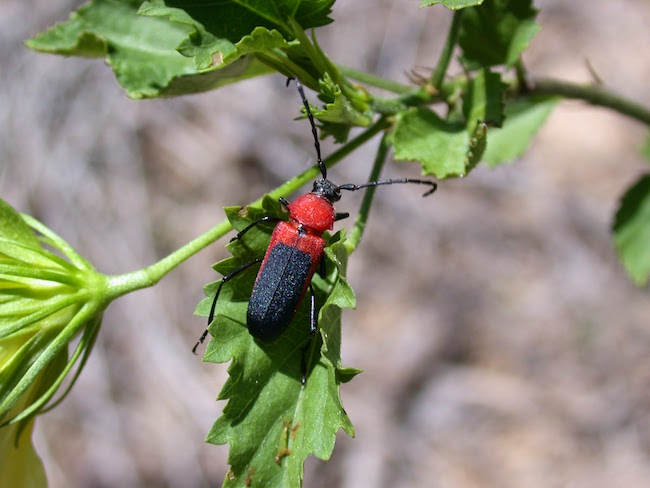
\includegraphics[keepaspectratio]{media/chapter_aov.jpg}}

\begin{quote}
If your data are taken from discrete groups (e.g., treatments), then we
are generally testing the equality of each group mean.
\end{quote}

\section{Lecture Materials}\label{lecture-materials-13}

\begin{quote}
\textbf{Lecture Slides:} Available interactively in the
\href{https://dyerlabteaching.github.io/Analysis-of-Variance/slides.html\#/title-slide}{online
version}
\end{quote}

\begin{figure}[H]

{\centering \pandocbounded{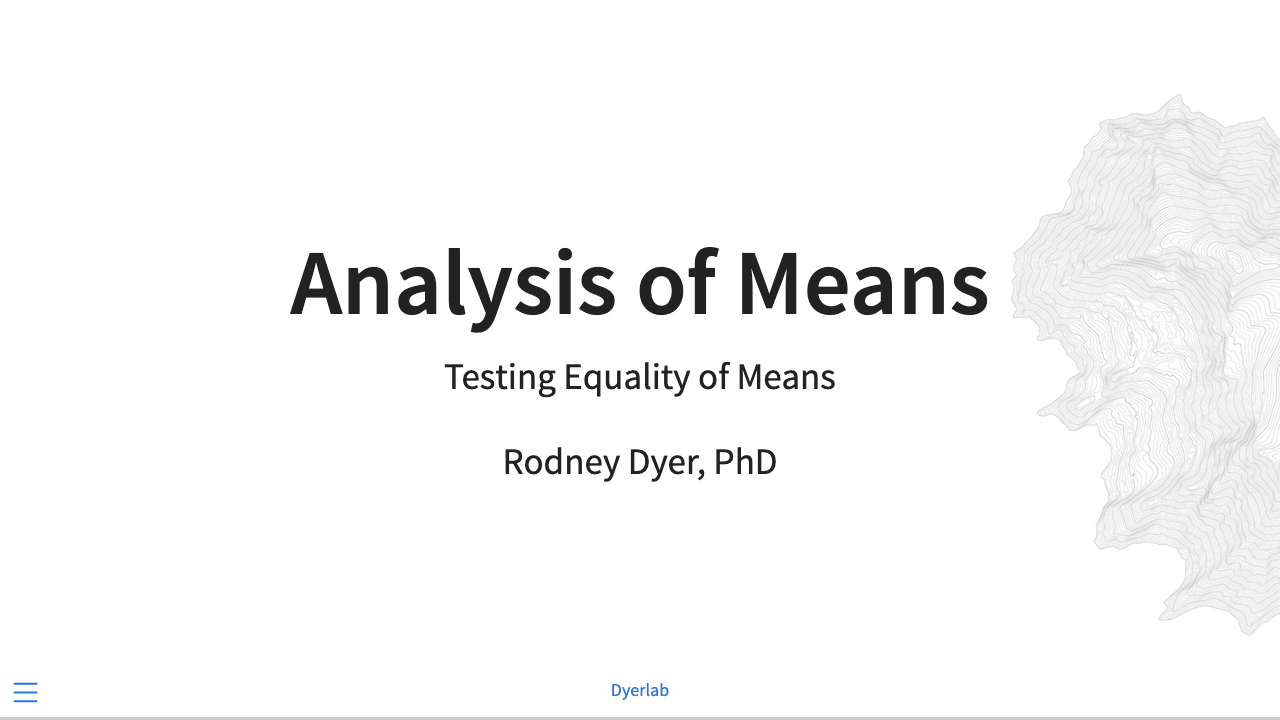
\includegraphics[keepaspectratio]{media/slides_aov.png}}

}

\caption{Lecture Slides}

\end{figure}%

Here we explore methods applicable to testing hypotheses about specific
parameters, as equal to a specified value (a \(t\)-test), equal between
two samples (paired \(t\)-tests), and equal among more than two groups
(analysis of variance).

In this and the next section, we will examine how to tell the difference
between measures of central tendency. This is applied to a single set of
data, pairs of data sets, and a data set with many different groups. As
we increase the complexity of these hypotheses, we will move through a
series of statistical tests, starting with a one-sample \(t\)-test, a
paired \(t\)-test, and then to the general analysis of variance (ANVOA)
approaches. All of these methods evaluate the equality of mean values.

\section{One Sample Hypotheses}\label{one-sample-hypotheses}

At the most basic level, we can take a set of data and test to see if
the mean of those values are equated to some particular value,
\(H_O: \mu = x\) (or \(H_O: \mu = 0\) in some cases). The idea here is
to determine, by specifying a value for the null hypothesis, what we
expect the mean value to be equal to. Going back to our idea of
hypothesis testing, the null hypothesis is the thing we are trying to
disprove (with some level of statistical confidence) and in doing so we
need to define a test statistic that we have an idea about its behavior.
In this case, we will define Student's \(t\)-test statistic as:

\(t =\frac{\bar{x}-\mu}{s_{\bar{x}}}\)

where \(\bar{x}\) is the observed mean of the data, \(\mu\) is the mean
value specified under the null hypothesis, and \(s_{\bar{x}}\) is the
standard deviation of the data. The value of the \(t\)-statistic can be
defined based upon the sample size (e.g., the degrees of freedom,
\(df\)). Here is what the probability density function looks like for
\(df = (1,3,\infty)\).

\begin{Shaded}
\begin{Highlighting}[]
\FunctionTok{library}\NormalTok{( ggplot2 )}
\NormalTok{x }\OtherTok{\textless{}{-}} \FunctionTok{seq}\NormalTok{(}\SpecialCharTok{{-}}\DecValTok{5}\NormalTok{,}\DecValTok{5}\NormalTok{,}\AttributeTok{by=}\FloatTok{0.02}\NormalTok{)}
\NormalTok{d }\OtherTok{\textless{}{-}} \FunctionTok{data.frame}\NormalTok{( }\AttributeTok{t=}\FunctionTok{c}\NormalTok{(x,x,x),}
                  \AttributeTok{f=}\FunctionTok{c}\NormalTok{(}\FunctionTok{dt}\NormalTok{(x,}\AttributeTok{df=}\DecValTok{1}\NormalTok{),}
                      \FunctionTok{dt}\NormalTok{(x,}\AttributeTok{df=}\DecValTok{3}\NormalTok{),}
                      \FunctionTok{dt}\NormalTok{(x,}\AttributeTok{df=}\ConstantTok{Inf}\NormalTok{)),}
                  \AttributeTok{df=}\FunctionTok{rep}\NormalTok{(}\FunctionTok{c}\NormalTok{(}\StringTok{"1"}\NormalTok{,}\StringTok{"3"}\NormalTok{,}\StringTok{"Inf"}\NormalTok{),}\AttributeTok{each=}\FunctionTok{length}\NormalTok{(x)))}
\FunctionTok{ggplot}\NormalTok{( d, }\FunctionTok{aes}\NormalTok{(}\AttributeTok{x=}\NormalTok{t,}\AttributeTok{y=}\NormalTok{f,}\AttributeTok{color=}\NormalTok{df)) }\SpecialCharTok{+} \FunctionTok{geom\_line}\NormalTok{() }
\end{Highlighting}
\end{Shaded}

\begin{center}
\pandocbounded{
\includegraphics[keepaspectratio]{narrative_aov_files/figure-pdf/unnamed-chunk-1-1.pdf}}
\end{center}

When \(df=\infty\) then \(PDF(t) = Normal\). As such, we do not need to
make corrections to understand the area under the curve, we can just use
the normal probability density function. In fact, when \(df=\infty\)
then \(t_{\alpha,\infty} = Z_{\alpha} = \sqrt{\chi^2_{\alpha,df=1}}\)!
The take home message here is that all your statistics become much
easier when \(N=\infty\), so go collect some more data!

For \(df < \infty\) (all the cases we will be dealing with), we will use
the approximation defined by the \(t\) distribution. If you look at the
distributions above, you see that as we increase the number of samples
(e.g., as \(df\) increases), the distribution becomes more restricted.
The actual function is defined (where \(df = v\) for simplicity in
nomenclature) as:

\(P(t|x,v)= \frac{ \Gamma\left( \frac{v+1}{2}\right)}{\sqrt{v\pi}\Gamma\left( \frac{v}{2}\right)} \left( 1 + \frac{x^2}{v}\right)^{-\frac{v+1}{2}}\)

where \(\Gamma\) is the Gamma function. Not pretty! Fortunately, we have
some built-in facilities in R that can make it easy for us.

For a single set of data, we can use the function above to estimate a
value of the \(t\) statistic. The probability distribution, defined by
the degrees of freedom, identifies regions within which we may suspect
the statistic to be abnormally large. In our case, though it is quite
arbitrary, we can define either one or two regions of the distribution
whose values would be extreme enough such that we would consider a
significant deviation. For a two-tailed test, the distribution below
illustrates this concept. If the estimated value of the \(t\) statistic
is in either of the shaded regions, we would reject the null hypothesis
of \(H_O: \mu = 0\) where \(\alpha=0.05\).

\begin{Shaded}
\begin{Highlighting}[]
\NormalTok{d1 }\OtherTok{\textless{}{-}} \FunctionTok{data.frame}\NormalTok{(}\AttributeTok{t=}\FunctionTok{c}\NormalTok{( }\FunctionTok{seq}\NormalTok{(}\SpecialCharTok{{-}}\DecValTok{5}\NormalTok{,}\SpecialCharTok{{-}}\FloatTok{2.064}\NormalTok{, }\AttributeTok{by=}\FloatTok{0.02}\NormalTok{), }\SpecialCharTok{{-}}\FloatTok{2.064}\NormalTok{, }\SpecialCharTok{{-}}\DecValTok{5}\NormalTok{), }
                 \AttributeTok{f=}\FunctionTok{c}\NormalTok{( }\FunctionTok{dt}\NormalTok{( }\FunctionTok{seq}\NormalTok{(}\SpecialCharTok{{-}}\DecValTok{5}\NormalTok{,}\SpecialCharTok{{-}}\FloatTok{2.064}\NormalTok{, }\AttributeTok{by=}\FloatTok{0.02}\NormalTok{),}\AttributeTok{df=}\DecValTok{1}\NormalTok{), }\FloatTok{0.01224269}\NormalTok{, }\FloatTok{0.01224269}\NormalTok{))}
\NormalTok{d2 }\OtherTok{\textless{}{-}} \FunctionTok{data.frame}\NormalTok{(}\AttributeTok{t=}\FunctionTok{c}\NormalTok{( }\FunctionTok{seq}\NormalTok{(}\FloatTok{2.064}\NormalTok{,}\DecValTok{5}\NormalTok{,}\AttributeTok{by=}\FloatTok{0.02}\NormalTok{), }\DecValTok{5}\NormalTok{, }\FloatTok{2.064}\NormalTok{),}
                 \AttributeTok{f=}\FunctionTok{c}\NormalTok{( }\FunctionTok{dt}\NormalTok{( }\FunctionTok{seq}\NormalTok{( }\FloatTok{2.064}\NormalTok{, }\DecValTok{5}\NormalTok{, }\AttributeTok{by=}\FloatTok{0.02}\NormalTok{),}\AttributeTok{df=}\DecValTok{1}\NormalTok{), }\FloatTok{0.01224269}\NormalTok{, }\FloatTok{0.01224269}\NormalTok{))}
\NormalTok{d3 }\OtherTok{\textless{}{-}} \FunctionTok{data.frame}\NormalTok{( }\AttributeTok{x=}\FunctionTok{c}\NormalTok{(}\FloatTok{2.5}\NormalTok{,}\SpecialCharTok{{-}}\FloatTok{2.5}\NormalTok{), }\AttributeTok{y=}\FloatTok{0.02719}\NormalTok{, }\AttributeTok{label=}\StringTok{"2.5\%"}\NormalTok{)}
\FunctionTok{ggplot}\NormalTok{() }\SpecialCharTok{+} 
  \FunctionTok{geom\_polygon}\NormalTok{(}\FunctionTok{aes}\NormalTok{(t,f),}\AttributeTok{data=}\NormalTok{d1, }\AttributeTok{fill=}\StringTok{"\#F8766D"}\NormalTok{,}\AttributeTok{alpha=}\FloatTok{0.5}\NormalTok{,}\AttributeTok{color=}\StringTok{"\#F8766D"}\NormalTok{) }\SpecialCharTok{+} 
  \FunctionTok{geom\_polygon}\NormalTok{(}\FunctionTok{aes}\NormalTok{(t,f),}\AttributeTok{data=}\NormalTok{d2, }\AttributeTok{fill=}\StringTok{"\#F8766D"}\NormalTok{,}\AttributeTok{alpha=}\FloatTok{0.5}\NormalTok{,}\AttributeTok{color=}\StringTok{"\#F8766D"}\NormalTok{) }\SpecialCharTok{+} 
  \FunctionTok{geom\_line}\NormalTok{( }\FunctionTok{aes}\NormalTok{(t,f),}\AttributeTok{data=}\NormalTok{d[d}\SpecialCharTok{$}\NormalTok{df}\SpecialCharTok{==}\DecValTok{1}\NormalTok{,], }\AttributeTok{color=}\StringTok{"\#F8766D"}\NormalTok{) }\SpecialCharTok{+} 
  \FunctionTok{geom\_text}\NormalTok{( }\FunctionTok{aes}\NormalTok{(x,y,}\AttributeTok{label=}\NormalTok{label),}\AttributeTok{data=}\NormalTok{d3)}
\end{Highlighting}
\end{Shaded}

\begin{center}
\pandocbounded{
\includegraphics[keepaspectratio]{narrative_aov_files/figure-pdf/unnamed-chunk-2-1.pdf}}
\end{center}

In R, we can use the \texttt{t.test()} function. I'm going to go back to
the \emph{Iris} data set and use that as it has three categories (the
species) and many measurements on sepals and pedals. Here I separate the
species into their own \texttt{data.frame} objects.

\begin{Shaded}
\begin{Highlighting}[]
\NormalTok{df.se }\OtherTok{\textless{}{-}}\NormalTok{ iris[ iris}\SpecialCharTok{$}\NormalTok{Species }\SpecialCharTok{==} \StringTok{"setosa"}\NormalTok{,] }
\NormalTok{df.ve }\OtherTok{\textless{}{-}}\NormalTok{ iris[ iris}\SpecialCharTok{$}\NormalTok{Species }\SpecialCharTok{==} \StringTok{"versicolor"}\NormalTok{,] }
\NormalTok{df.vi }\OtherTok{\textless{}{-}}\NormalTok{ iris[ iris}\SpecialCharTok{$}\NormalTok{Species }\SpecialCharTok{==} \StringTok{"virginica"}\NormalTok{,]}
\end{Highlighting}
\end{Shaded}

Lets look at the \texttt{Sepal.Length} feature in these species and
create some hypotheses about it.

\begin{Shaded}
\begin{Highlighting}[]
\FunctionTok{ggplot}\NormalTok{( iris, }\FunctionTok{aes}\NormalTok{(}\AttributeTok{x=}\NormalTok{Sepal.Length, }\AttributeTok{fill=}\NormalTok{Species)) }\SpecialCharTok{+} \FunctionTok{geom\_density}\NormalTok{(}\AttributeTok{alpha=}\FloatTok{0.75}\NormalTok{)}
\end{Highlighting}
\end{Shaded}

\begin{center}
\pandocbounded{
\includegraphics[keepaspectratio]{narrative_aov_files/figure-pdf/unnamed-chunk-4-1.pdf}}
\end{center}

We could test the hypothesis, \(H_O: mean(Sepal.Length)=6\) for each of
the species.

\begin{Shaded}
\begin{Highlighting}[]
\NormalTok{fit.se }\OtherTok{\textless{}{-}} \FunctionTok{t.test}\NormalTok{(df.se}\SpecialCharTok{$}\NormalTok{Sepal.Length, }\AttributeTok{mu =} \FloatTok{6.0}\NormalTok{)}
\NormalTok{fit.se}
\end{Highlighting}
\end{Shaded}

\begin{verbatim}

    One Sample t-test

data:  df.se$Sepal.Length
t = -19.94, df = 49, p-value < 2.2e-16
alternative hypothesis: true mean is not equal to 6
95 percent confidence interval:
 4.905824 5.106176
sample estimates:
mean of x 
    5.006 
\end{verbatim}

From the output, it appears that we can reject that null hypothesis
(\(t =\) -19.9; \(df =\) 49; \(P =\) 3.7e-25).

For \emph{I. versicolor}, we see that the mean does appear to be equal
to 6.0 (and thus fail to reject the null hypothesis):

\begin{Shaded}
\begin{Highlighting}[]
\FunctionTok{t.test}\NormalTok{( df.ve}\SpecialCharTok{$}\NormalTok{Sepal.Length, }\AttributeTok{mu=}\FloatTok{6.0}\NormalTok{ )}
\end{Highlighting}
\end{Shaded}

\begin{verbatim}

    One Sample t-test

data:  df.ve$Sepal.Length
t = -0.87674, df = 49, p-value = 0.3849
alternative hypothesis: true mean is not equal to 6
95 percent confidence interval:
 5.789306 6.082694
sample estimates:
mean of x 
    5.936 
\end{verbatim}

and for \emph{I. virginica}, we find that it is significantly larger
than 6.0 and again reject the null hypothesis:

\begin{Shaded}
\begin{Highlighting}[]
\FunctionTok{t.test}\NormalTok{( df.vi}\SpecialCharTok{$}\NormalTok{Sepal.Length, }\AttributeTok{mu=}\FloatTok{6.0}\NormalTok{ )}
\end{Highlighting}
\end{Shaded}

\begin{verbatim}

    One Sample t-test

data:  df.vi$Sepal.Length
t = 6.5386, df = 49, p-value = 3.441e-08
alternative hypothesis: true mean is not equal to 6
95 percent confidence interval:
 6.407285 6.768715
sample estimates:
mean of x 
    6.588 
\end{verbatim}

In all the output, we are also given an estimate of the Confidence
Interval around the mean. This confidence interval is determined as:

\(\bar{x} - t_{\alpha, df} s_{\bar{x}} < \mu < \bar{x} + t_{\alpha, df} s_{\bar{x}}\)

or the mean plus or minus standard deviation of the data times the value
of the \(t\)-statistic for a given level of \(\alpha\) and \(df\).

\subsection{Data Variability}\label{data-variability}

There are times when reporting some confidence around a parameter is
important, particularly when using tabular data as output.

\begin{Shaded}
\begin{Highlighting}[]
\NormalTok{Species }\OtherTok{\textless{}{-}} \FunctionTok{c}\NormalTok{(}\StringTok{"Iris setosa"}\NormalTok{,}\StringTok{"Iris versicolor"}\NormalTok{,}\StringTok{"Iris virginia"}\NormalTok{)}
\NormalTok{Sepal.Length }\OtherTok{\textless{}{-}} \FunctionTok{c}\NormalTok{(}\FunctionTok{mean}\NormalTok{(df.se}\SpecialCharTok{$}\NormalTok{Sepal.Length), }\FunctionTok{mean}\NormalTok{(df.ve}\SpecialCharTok{$}\NormalTok{Sepal.Length), }\FunctionTok{mean}\NormalTok{( df.vi}\SpecialCharTok{$}\NormalTok{Sepal.Length))}
\NormalTok{Sepal.Length.SE }\OtherTok{\textless{}{-}} \FunctionTok{c}\NormalTok{(}\FunctionTok{sd}\NormalTok{(df.se}\SpecialCharTok{$}\NormalTok{Sepal.Length), }\FunctionTok{sd}\NormalTok{(df.ve}\SpecialCharTok{$}\NormalTok{Sepal.Length), }\FunctionTok{sd}\NormalTok{( df.vi}\SpecialCharTok{$}\NormalTok{Sepal.Length))}
\NormalTok{Sepal.Length.SEM }\OtherTok{\textless{}{-}}\NormalTok{ Sepal.Length.SE }\SpecialCharTok{/} \FunctionTok{sqrt}\NormalTok{(}\DecValTok{50}\NormalTok{)}
\end{Highlighting}
\end{Shaded}

There are two ways we can talk about the data and it is important for
you to think about what you are trying to communicate to your readers.
These alternatives include:

\begin{Shaded}
\begin{Highlighting}[]
\NormalTok{sd }\OtherTok{\textless{}{-}} \FunctionTok{paste}\NormalTok{( }\FunctionTok{format}\NormalTok{(Sepal.Length,}\AttributeTok{digits=}\DecValTok{2}\NormalTok{), }\StringTok{"+/{-}"}\NormalTok{, }\FunctionTok{format}\NormalTok{(Sepal.Length.SE, }\AttributeTok{digits=}\DecValTok{3}\NormalTok{))}
\NormalTok{se }\OtherTok{\textless{}{-}} \FunctionTok{paste}\NormalTok{( }\FunctionTok{format}\NormalTok{(Sepal.Length,}\AttributeTok{digits=}\DecValTok{2}\NormalTok{), }\StringTok{"+/{-}"}\NormalTok{, }\FunctionTok{format}\NormalTok{(Sepal.Length.SEM, }\AttributeTok{digits=}\DecValTok{3}\NormalTok{))}
\NormalTok{df }\OtherTok{\textless{}{-}} \FunctionTok{data.frame}\NormalTok{( Species, sd, se )}
\FunctionTok{names}\NormalTok{(df) }\OtherTok{\textless{}{-}} \FunctionTok{c}\NormalTok{(}\StringTok{"Species"}\NormalTok{,}\StringTok{"Mean +/{-} SD"}\NormalTok{, }\StringTok{"Sepal Length +/{-} SE"}\NormalTok{)}
\NormalTok{knitr}\SpecialCharTok{::}\FunctionTok{kable}\NormalTok{(df,}\AttributeTok{row.names =} \ConstantTok{FALSE}\NormalTok{,}\AttributeTok{digits =} \DecValTok{3}\NormalTok{,}\AttributeTok{align =} \StringTok{"lcc"}\NormalTok{)}
\end{Highlighting}
\end{Shaded}

{\def\LTcaptype{none} % do not increment counter
\begin{longtable}[]{@{}lcc@{}}
\toprule\noalign{}
Species & Mean +/- SD & Sepal Length +/- SE \\
\midrule\noalign{}
\endhead
\bottomrule\noalign{}
\endlastfoot
Iris setosa & 5.0 +/- 0.352 & 5.0 +/- 0.0498 \\
Iris versicolor & 5.9 +/- 0.516 & 5.9 +/- 0.0730 \\
Iris virginia & 6.6 +/- 0.636 & 6.6 +/- 0.0899 \\
\end{longtable}
}

The two columns of data tell us something different. The middle column
tells us the mean and the standard deviation of the data. This tells us
about the variability (and confidence) of the data itself. The last
column is the Standard Error of the Mean (\(\frac{s}{\sqrt{N}}\)) and
gives us an idea of the confidence we have about the \emph{mean}
estimate of the data (as opposed to the variation of the data itself).
These are two different statements about the data and you need to make
sure you are confident about which way you want to use to communicate to
your audience.

\section{Two Sample Hypotheses}\label{two-sample-hypotheses}

In addition to a single sample test, evaluating if the mean of a set of
data is equal to some specified value, we can test the equality of two
different samples. It may be the case that the average sepal length for
\emph{I. versicolor} is not significantly different than 6.0 whereas
\emph{I. virginia} is. However, this does not mean that the mean of both
of these species are significantly different from each other. This is a
two-sampled hypothesis, stating that \(H_O: \mu_X = \mu_Y\).

Visually, these data look like:

\begin{Shaded}
\begin{Highlighting}[]
\NormalTok{df }\OtherTok{\textless{}{-}}\NormalTok{ iris[ (iris}\SpecialCharTok{$}\NormalTok{Species }\SpecialCharTok{\%in\%} \FunctionTok{c}\NormalTok{(}\StringTok{"versicolor"}\NormalTok{,}\StringTok{"virginica"}\NormalTok{)),]}
\FunctionTok{ggplot}\NormalTok{( df, }\FunctionTok{aes}\NormalTok{(}\AttributeTok{x=}\NormalTok{Species, }\AttributeTok{y=}\NormalTok{Sepal.Length)) }\SpecialCharTok{+} \FunctionTok{geom\_boxplot}\NormalTok{(}\AttributeTok{notch=}\ConstantTok{TRUE}\NormalTok{)}
\end{Highlighting}
\end{Shaded}

\begin{center}
\pandocbounded{
\includegraphics[keepaspectratio]{narrative_aov_files/figure-pdf/unnamed-chunk-10-1.pdf}}
\end{center}

which clearly overlap in their distributions but are the mean values
different? This sets up the null hypothesis:

\(H_O: \mu_1 - \mu_2 = 0\)

Under this hypothesis, we can use a \emph{t}-test like before but just
rearranged as:

\(t = \frac{\bar{x}_1 - \bar{x}_2}{s_{\bar{x}_1-\bar{x}_2}}\)

As before, if the difference in the numerator is small we would reject
but here we need to standardize the differences in the means by a
measure of the standard deviation that is based upon both sets of data.
This is called a the \emph{standard error of the difference in two
means} (real catchy title, no?). This is defined as:

\(s_{\bar{x}_1-\bar{x}_2} = \sqrt{ \frac{s_1^2}{N_1}+\frac{s_2^2}{N}}\)

To test this, we use the same approach as before but instead of defining
\(\mu = 6.0\) in the \texttt{t.test()} function, we instead give it both
data sets.

\begin{Shaded}
\begin{Highlighting}[]
\FunctionTok{t.test}\NormalTok{( }\AttributeTok{x=}\NormalTok{df.vi}\SpecialCharTok{$}\NormalTok{Sepal.Length, }\AttributeTok{y =}\NormalTok{ df.ve}\SpecialCharTok{$}\NormalTok{Sepal.Length )}
\end{Highlighting}
\end{Shaded}

\begin{verbatim}

    Welch Two Sample t-test

data:  df.vi$Sepal.Length and df.ve$Sepal.Length
t = 5.6292, df = 94.025, p-value = 1.866e-07
alternative hypothesis: true difference in means is not equal to 0
95 percent confidence interval:
 0.4220269 0.8819731
sample estimates:
mean of x mean of y 
    6.588     5.936 
\end{verbatim}

Here we get a few bits of new information from the analysis. It is
obvious that we would reject the null hypothesis given the magnitude of
the estimated \(P\)-value. The output also provides us an estimate of
the mean values for each group as well as the confidence around the
difference in the mean values. This confidence interval does not overlap
0.0, as it shouldn't if we reject \(H_O: \mu_X = \mu_Y\).

\section{Many Sample Hypotheses}\label{many-sample-hypotheses}

If we have more than two samples, we could do a bunch of paired
\(t\)-test statistics but this is not the best idea. In fact, if we do
this to our data, each time testing at a confidence level of, say,
\(\alpha = 0.05\), then for each time we test at \(0.05\) but over all
pairs, we test at an overall level of \(0.05^k\) (where \(k\) is the
number of tests) value. We cannot do multiple tests without penalizing
ourselves in terms of the level at which we consider something
significant if we are going to do all these tests. You may have heard
about a Bonferroni correction---this does exactly that, it allows us to
modify the \(\alpha\) level we use to take into consideration the number
of tests we are going to use. While this may be an acceptable way to
test for the equality of several means (and it may not actually be if
you ask most statisticians), there is another way that is much easier.

Consider the case where we have many categories (e.g., factors in R)
that we are interested in determining if the mean of all are equal. The
null hypothesis for this is, \(H_O: \mu_1 = \mu_2 = \ldots = \mu_k\),
where there are \(k\) different treatment levels. This is essentially
what we'd want to do by doing a bunch of \(t\)-tests but we can use
another approach that we don't have to penalize ourselves for multiple
tests. Here is how it works.

In the \emph{Iris} data, we can visualize the means and variation around
them by using box plots. Here is an example.

\begin{Shaded}
\begin{Highlighting}[]
\FunctionTok{ggplot}\NormalTok{( iris, }\FunctionTok{aes}\NormalTok{(}\AttributeTok{x=}\NormalTok{Species, }\AttributeTok{y=}\NormalTok{Sepal.Length)) }\SpecialCharTok{+} 
  \FunctionTok{geom\_boxplot}\NormalTok{(}\AttributeTok{notch =} \ConstantTok{TRUE}\NormalTok{) }\SpecialCharTok{+} 
  \FunctionTok{ylab}\NormalTok{(}\StringTok{"Sepal Length"}\NormalTok{)}
\end{Highlighting}
\end{Shaded}

\begin{center}
\pandocbounded{
\includegraphics[keepaspectratio]{narrative_aov_files/figure-pdf/unnamed-chunk-12-1.pdf}}
\end{center}

For us to tell if there are statistical differences among the species,
we need to look at both the location of the mean values as well as the
variation around them. We do this by partitioning the variation in all
the data into the components within each treatment (species) and among
each treatment (species) using an approach derived from the sum of
squared deviations (or Sums of Squares). Formally, we can estimate the
sum of squares within each of the \(K\) groupings as:

\(SS_{Within} = \sum_{i=1}^K\left( \sum_{j=1}^{N_i}(x_{ij}-\bar{x}_i)^2 \right)\)

whose degrees of freedom are defined as:

\(df_{W} = \sum_{i=1}^K \left( N_i - 1 \right) = N-K\)

These parameters represent the deviation among samples within groups and
the number of independent samples within these groups. We also need to
partition out the variation among groups as a similarly defined Sums of
Squares:

\(SS_{Among} = \sum_{i=1}^K N_i\left( \bar{x}_i - \bar{x} \right)^2\)

or the deviation among the mean of each treatment compared to the
overall mean of all the data. This parameter has degrees of freedom
equal to

\(df_{A} = K - 1\)

These two parameters describe all the data and as such
\(SS_{Total} = SS_{Within} + SS_{Among}\). Formally, we see that

\(SS_{Total} = \sum_{i=1}^K\sum_{j=1}^{N_i} (x_{ij} - \bar{x})^2\)

whose degrees of freedom are

\(df_{T} = N - 1\)

For each of these Sums of Squared deviations, we can standardize them
using the degrees of freedom. The notion here is that with more samples,
and more treatments, we will have greater \(SS\) values. However, if we
standardize these parameters by the \(df\), we can come up with a
standardized Mean Squared values (simplified as \(MS = \frac{SS}{df}\)
for each level).

If we look at all these values, we can create the venerable ANOVA table
with Among, Within, and Total partitions of the variation.

{\def\LTcaptype{none} % do not increment counter
\begin{longtable}[]{@{}
  >{\raggedright\arraybackslash}p{(\linewidth - 6\tabcolsep) * \real{0.0611}}
  >{\raggedright\arraybackslash}p{(\linewidth - 6\tabcolsep) * \real{0.0534}}
  >{\raggedright\arraybackslash}p{(\linewidth - 6\tabcolsep) * \real{0.5191}}
  >{\raggedright\arraybackslash}p{(\linewidth - 6\tabcolsep) * \real{0.3664}}@{}}
\toprule\noalign{}
\begin{minipage}[b]{\linewidth}\raggedright
Source
\end{minipage} & \begin{minipage}[b]{\linewidth}\raggedright
df
\end{minipage} & \begin{minipage}[b]{\linewidth}\raggedright
SS
\end{minipage} & \begin{minipage}[b]{\linewidth}\raggedright
MS
\end{minipage} \\
\midrule\noalign{}
\endhead
\bottomrule\noalign{}
\endlastfoot
Among & \(K-1\) &
\(\sum_{i=1}^K N_i \left( \bar{x}_i - \bar{x} \right)^2\) &
\(\frac{SS_A}{K-1}\) \\
Within & \(N-K\) &
\(\sum_{i=1}^Kn_i\left( \sum_{j=1}^{N_i}(x_{ij}-\bar{x}_i)^2 \right)\) &
\(\frac{SS_W}{N-K}\) \\
Total & \(N-1\) & \(\sum_{i=1}^K \sum_{j=1}^{N_i} (x_{ij} - \bar{x})^2\)
& \\
\end{longtable}
}

In R, we can evaluate the equality of means by partitioning our data as
depicted above. Essentially, if at least one of our treatments means
deviate significantly, then the \(MS_A\) will be abnormally large
relative to the variation within each treatment \(MS_W\). This gives us
a statistic, defined by the American statistician Snedekor as:

\(F = \frac{MS_A}{MS_W}\)

as an homage to Ronald Fisher (the F-statistic) has a pretty well
understood distribution under a few conditions. This statistic has an
expectation of:

\(f(x | df_A, df_W) = \frac{\sqrt{\frac{(df_Ax)^{df_A}df_W^{df_W}}{(df_Ax + df_W)^{df_W+df_A}}}}{x\mathbf{B}\left( \frac{df_A}{2}, \frac{df_W}{2} \right)}\)

which is even more of a mess than that for the \(t\)-test! Luckily, we
have a bit of code to do this for us.

Here is an example using the \emph{Iris} data. Here we test the
hypothesis that the Sepal Lengths are all the same (e.g.,
\(H_O: \mu_{se} = \mu_{ve} = \mu_{vi}\))

\begin{Shaded}
\begin{Highlighting}[]
\NormalTok{fit.aov }\OtherTok{\textless{}{-}} \FunctionTok{aov}\NormalTok{( Sepal.Length }\SpecialCharTok{\textasciitilde{}}\NormalTok{ Species, }\AttributeTok{data=}\NormalTok{iris)}
\NormalTok{fit.aov}
\end{Highlighting}
\end{Shaded}

\begin{verbatim}
Call:
   aov(formula = Sepal.Length ~ Species, data = iris)

Terms:
                 Species Residuals
Sum of Squares  63.21213  38.95620
Deg. of Freedom        2       147

Residual standard error: 0.5147894
Estimated effects may be unbalanced
\end{verbatim}

The function called here, \texttt{aov()} is the one that does the
Analysis of Variance. It returns an object that has the necessary data
we need. To estimate the ANOVA table as outlined above we ask for it as:

\begin{Shaded}
\begin{Highlighting}[]
\FunctionTok{anova}\NormalTok{(fit.aov)}
\end{Highlighting}
\end{Shaded}

\begin{verbatim}
Analysis of Variance Table

Response: Sepal.Length
           Df Sum Sq Mean Sq F value    Pr(>F)    
Species     2 63.212  31.606  119.26 < 2.2e-16 ***
Residuals 147 38.956   0.265                      
---
Signif. codes:  0 '***' 0.001 '**' 0.01 '*' 0.05 '.' 0.1 ' ' 1
\end{verbatim}

which shows that the ``Species'' treatment are significantly different
from each other, with an \(F\) statistic equal to \(F = 119.3\), which
with 2 and 147 degrees of freedom is assigned a probability equal to
\(2e^{-16}\), a very small value!

\subsection{Post-Hoc Tests}\label{post-hoc-tests}

What this analysis tells us is that \emph{at least} one of the treatment
means are different from the rest. What it does not tell us is which one
or which subset. It could be that \emph{I. setosa} is significantly
smaller than both \emph{I. versitosa} and \emph{I. virginia}. It could
be that \emph{I. virginia} is significantly larger than the others, who
are not different. It could also mean that they are all different. To
address this, we can estimate a \emph{post hoc} test, to evaluate the
difference between treatment means within this model itself.

One of the most common ways to evaluate the equality of treatment mean
values is that defined by Tukey. The so-called ``Honest Significant
Differences'' \emph{post hoc} test is given by

\begin{Shaded}
\begin{Highlighting}[]
\NormalTok{tuk }\OtherTok{\textless{}{-}} \FunctionTok{TukeyHSD}\NormalTok{(fit.aov)}
\NormalTok{tuk}
\end{Highlighting}
\end{Shaded}

\begin{verbatim}
  Tukey multiple comparisons of means
    95% family-wise confidence level

Fit: aov(formula = Sepal.Length ~ Species, data = iris)

$Species
                      diff       lwr       upr p adj
versicolor-setosa    0.930 0.6862273 1.1737727     0
virginica-setosa     1.582 1.3382273 1.8257727     0
virginica-versicolor 0.652 0.4082273 0.8957727     0
\end{verbatim}

which breaks down the pair-wise differences in the mean of each
treatment. Here we see the magnitude of the differences in mean values,
the lower and upper confidence on the differences, and the probability
associated with these differences. In this example, all three
comparisons are highly unlikely (e.g., \(P\) is very small and in this
case essentially zero). As a result, we can interpret these results as
suggesting that each of the three species have significantly different.
If we plot these results, we see which ones are larger and which are
smaller.

\begin{Shaded}
\begin{Highlighting}[]
\FunctionTok{plot}\NormalTok{( tuk )}
\end{Highlighting}
\end{Shaded}

\begin{center}
\pandocbounded{
\includegraphics[keepaspectratio]{narrative_aov_files/figure-pdf/unnamed-chunk-16-1.pdf}}
\end{center}

Which shows the difference between treatment mean between all pairs of
treatments. Overall, we see that the \emph{Iris} species are all
significantly different.

\chapter{Ordination}\label{ordination}

\pandocbounded{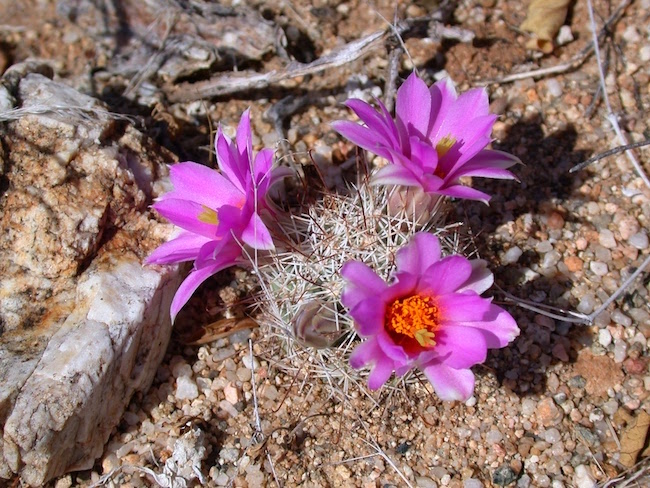
\includegraphics[keepaspectratio]{media/chapter_ordination.jpg}}

\begin{quote}
Ordination is a technique to take high-dimensional data and to represent
it in a lower dimensional context.
\end{quote}

\section{Lecture Materials}\label{lecture-materials-14}

\begin{quote}
\textbf{Lecture Slides:} Available interactively in the
\href{https://dyerlabteaching.github.io/Ordination/slides.html\#/title-slide}{online
version}
\end{quote}

\begin{figure}[H]

{\centering \pandocbounded{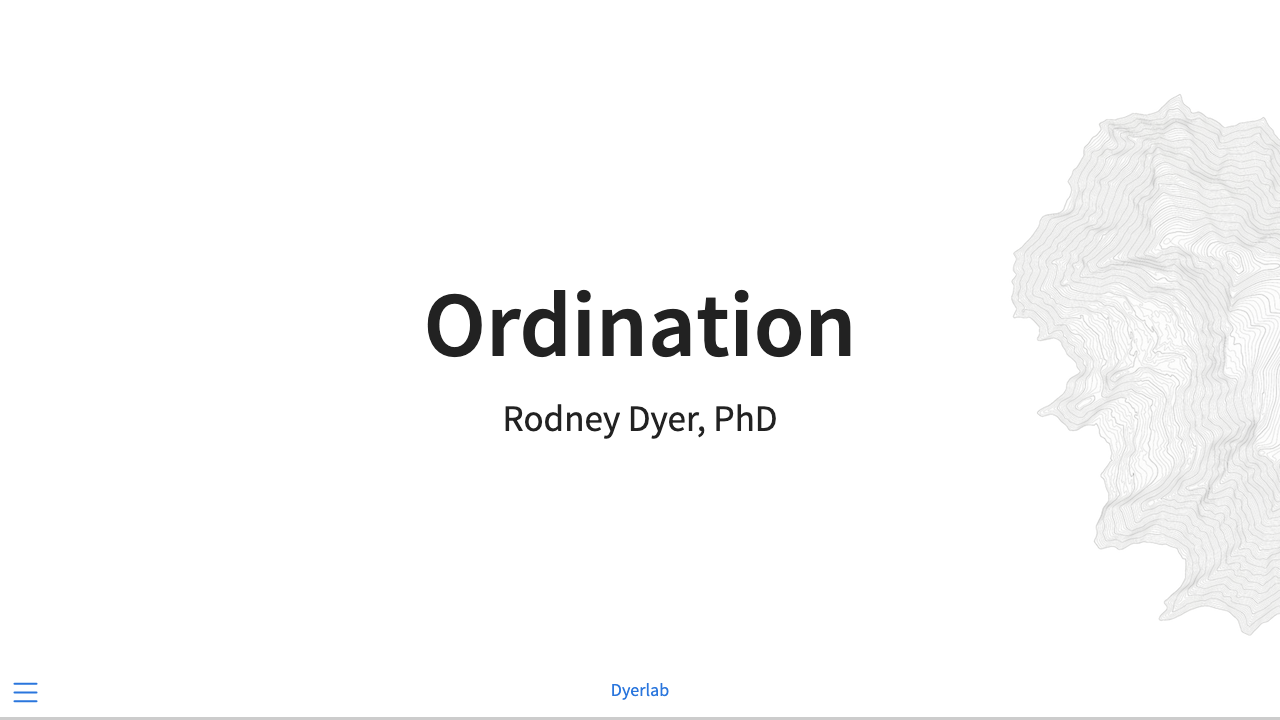
\includegraphics[keepaspectratio]{media/slides_ordination.png}}

}

\caption{Lecture Slides}

\end{figure}%

Ordination is a collective term for multivariate techniques which
summarize a multidimensional dataset in such a way that when it is
projected onto a low dimensional space, any intrinsic pattern the data
may possess becomes apparent upon visual inspection\footnote{Pielou EC,
  (1984) The interpretation of ecological data: A primer on
  classification and ordination. 288pg. ISBN:
  \href{https://www.wiley.com/en-us/The+Interpretation+of+Ecological+Data\%3A+A+Primer+on+Classification+and+Ordination-p-9780471889502}{978-0-471-88950-2}}.

One of the largest challenges in data analysis is the ability to
understand and gain inferences from it! This is especially compounded
when we have many different kinds of data describing our individual
observations. For example, at a particular vernal pool, we may have
measured pool size, pool depth, elevation, rainfall, temperature, canopy
cover, pH, aquatic vegitation, species1 density, species2 density, etc.
To describe all of these variables we could either plot all combinations
of them \emph{or} be a bit clever and use some ordination approaches.

For this activity, I am going to use the beer styles as a data set in
explaining a couple of different types of ordination. It is available as
the raw CSV file.

\begin{Shaded}
\begin{Highlighting}[]
\NormalTok{url }\OtherTok{\textless{}{-}} \StringTok{"https://raw.githubusercontent.com/dyerlab/ENVS{-}Lectures/master/data/Beer\_Styles.csv"}
\FunctionTok{read\_csv}\NormalTok{( url ) }\SpecialCharTok{\%\textgreater{}\%}
  \FunctionTok{mutate}\NormalTok{( }\AttributeTok{Yeast =} \FunctionTok{as.factor}\NormalTok{( Yeast ) ) }\OtherTok{{-}\textgreater{}}\NormalTok{ data}
\FunctionTok{summary}\NormalTok{(data)}
\end{Highlighting}
\end{Shaded}

\begin{verbatim}
    Styles             Yeast       ABV_Min         ABV_Max      
 Length:100         Ale   :69   Min.   :2.400   Min.   : 3.200  
 Class :character   Either: 4   1st Qu.:4.200   1st Qu.: 5.475  
 Mode  :character   Lager :27   Median :4.600   Median : 6.000  
                                Mean   :4.947   Mean   : 6.768  
                                3rd Qu.:5.500   3rd Qu.: 8.000  
                                Max.   :9.000   Max.   :14.000  
    IBU_Min         IBU_Max          SRM_Min         SRM_Max     
 Min.   : 0.00   Min.   :  8.00   Min.   : 2.00   Min.   : 3.00  
 1st Qu.:15.00   1st Qu.: 25.00   1st Qu.: 3.50   1st Qu.: 7.00  
 Median :20.00   Median : 35.00   Median : 8.00   Median :17.00  
 Mean   :21.97   Mean   : 38.98   Mean   : 9.82   Mean   :17.76  
 3rd Qu.:25.00   3rd Qu.: 45.00   3rd Qu.:14.00   3rd Qu.:22.00  
 Max.   :60.00   Max.   :120.00   Max.   :30.00   Max.   :40.00  
     OG_Min          OG_Max          FG_Min          FG_Max     
 Min.   :1.026   Min.   :1.032   Min.   :0.998   Min.   :1.006  
 1st Qu.:1.040   1st Qu.:1.052   1st Qu.:1.008   1st Qu.:1.012  
 Median :1.046   Median :1.060   Median :1.010   Median :1.015  
 Mean   :1.049   Mean   :1.065   Mean   :1.009   Mean   :1.016  
 3rd Qu.:1.056   3rd Qu.:1.075   3rd Qu.:1.010   3rd Qu.:1.018  
 Max.   :1.080   Max.   :1.130   Max.   :1.020   Max.   :1.040  
\end{verbatim}

These data give ranges of values but it is probably easier if we just
take the midpoint of the range.

\begin{Shaded}
\begin{Highlighting}[]
\NormalTok{data }\SpecialCharTok{\%\textgreater{}\%}
  \FunctionTok{mutate}\NormalTok{( }\AttributeTok{ABV=}\NormalTok{( ABV\_Max}\SpecialCharTok{+}\NormalTok{ABV\_Min)}\SpecialCharTok{/}\DecValTok{2}\NormalTok{,}
          \AttributeTok{IBU=}\NormalTok{( IBU\_Max}\SpecialCharTok{+}\NormalTok{IBU\_Min)}\SpecialCharTok{/}\DecValTok{2}\NormalTok{,}
          \AttributeTok{SRM=}\NormalTok{( SRM\_Max}\SpecialCharTok{+}\NormalTok{SRM\_Min)}\SpecialCharTok{/}\DecValTok{2}\NormalTok{,}
          \AttributeTok{OG=}\NormalTok{( OG\_Max}\SpecialCharTok{+}\NormalTok{OG\_Min)}\SpecialCharTok{/}\DecValTok{2}\NormalTok{,}
          \AttributeTok{FG=}\NormalTok{( FG\_Max}\SpecialCharTok{+}\NormalTok{FG\_Min)}\SpecialCharTok{/}\DecValTok{2}\NormalTok{ )  }\SpecialCharTok{\%\textgreater{}\%}
  \FunctionTok{select}\NormalTok{( Styles, Yeast, ABV, IBU, SRM, OG, FG) }\OtherTok{{-}\textgreater{}}\NormalTok{ beers}
\FunctionTok{summary}\NormalTok{( beers)}
\end{Highlighting}
\end{Shaded}

\begin{verbatim}
    Styles             Yeast         ABV              IBU       
 Length:100         Ale   :69   Min.   : 2.850   Min.   : 5.00  
 Class :character   Either: 4   1st Qu.: 4.900   1st Qu.:21.38  
 Mode  :character   Lager :27   Median : 5.300   Median :26.25  
                                Mean   : 5.857   Mean   :30.48  
                                3rd Qu.: 6.750   3rd Qu.:37.50  
                                Max.   :11.500   Max.   :90.00  
      SRM              OG              FG       
 Min.   : 2.50   Min.   :1.030   Min.   :1.003  
 1st Qu.: 5.00   1st Qu.:1.047   1st Qu.:1.010  
 Median :12.75   Median :1.052   Median :1.012  
 Mean   :13.79   Mean   :1.057   Mean   :1.013  
 3rd Qu.:18.00   3rd Qu.:1.065   3rd Qu.:1.014  
 Max.   :35.00   Max.   :1.100   Max.   :1.029  
\end{verbatim}

Excellent. If we look a the data now, we can see that there are a
moderate amount of correlation between data types and all of the
characteristics are spread reasonably well across the Yeast types. Here
is a pairwise plot of all the data using the \texttt{GGally::ggpairs()}
function.

\begin{Shaded}
\begin{Highlighting}[]
\FunctionTok{library}\NormalTok{(GGally)}
\NormalTok{beers }\SpecialCharTok{\%\textgreater{}\%}
  \FunctionTok{select}\NormalTok{( }\SpecialCharTok{{-}}\NormalTok{Styles ) }\SpecialCharTok{\%\textgreater{}\%}
  \FunctionTok{ggpairs}\NormalTok{() }
\end{Highlighting}
\end{Shaded}

\begin{center}
\pandocbounded{
\includegraphics[keepaspectratio]{narrative_ordination_files/figure-pdf/unnamed-chunk-3-1.pdf}}
\end{center}

\section{Principle Component
Analyses}\label{principle-component-analyses}

Principle component analysis (PCA) is a translation of the original data
into new coordinate spaces. This has absolutely nothing to do with the
relationship among the data themselves but is more of a way to create
new coordinates for each data point under the following criteria:\\
1. The number of axes in the translated data are the same as the number
of axes in the original data. 2. Axes are chosen by taking all the data
and finding transects through it that account for the broadest variation
in the data. 3. Each axis is defined as a linear combination of the
original axes. 3. Subsequent axes \emph{must be} orthoganal to all
previous ones (e.g., at 90\(\deg\) angles). 4. The amount of the total
variation in the system can be partitioned by these new axes and they
are ordered from those that explain the most variation to those who
explain the least.

An exmaple of this rotation is given below.

\begin{figure}[H]

{\centering \pandocbounded{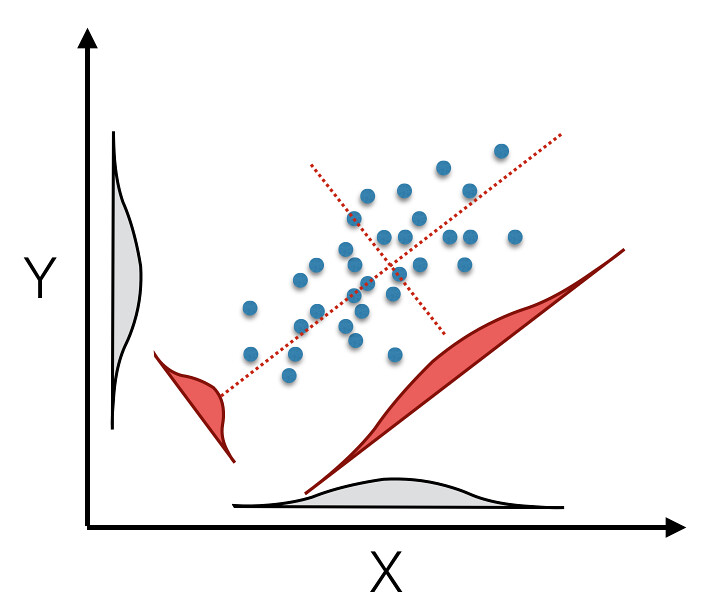
\includegraphics[keepaspectratio]{media/pca_rotation.jpg}}

}

\caption{A rotation of 2-dimenational data from the original coordinate
space (represented by the x- and y-axes) onto synthetic principal
component (the red axes). The rotation itself maximizes the
distributional width of the data (depicted as density plots in grey for
the original axes and red for the rotated axes).}

\end{figure}%

To conduct this rotation on our data, we use the function
\texttt{prcomp()}. It does the rotation and returns an analysis object
that has all the information we need in it.

\begin{Shaded}
\begin{Highlighting}[]
\NormalTok{pc.fit }\OtherTok{\textless{}{-}} \FunctionTok{prcomp}\NormalTok{(beers[,}\DecValTok{3}\SpecialCharTok{:}\DecValTok{7}\NormalTok{])}
\FunctionTok{names}\NormalTok{( pc.fit)}
\end{Highlighting}
\end{Shaded}

\begin{verbatim}
[1] "sdev"     "rotation" "center"   "scale"    "x"       
\end{verbatim}

If we look at the raw analysis output, we see a summary of the amount of
data explained by each of the axes as well as the loadings (e.g., the
linear combinations of the original data that translate the old
coordinates into the new ones).

\begin{Shaded}
\begin{Highlighting}[]
\NormalTok{pc.fit}
\end{Highlighting}
\end{Shaded}

\begin{verbatim}
Standard deviations (1, .., p=5):
[1] 17.407474934  8.593744939  1.537237291  0.004779020  0.001954314

Rotation (n x k) = (5 x 5):
             PC1           PC2          PC3           PC4           PC5
ABV 0.0500642463  0.0005333582 -0.998701196 -8.619900e-03 -3.860675e-03
IBU 0.9773017876  0.2060831568  0.049101404  9.539617e-06  2.089354e-05
SRM 0.2058507906 -0.9785343146  0.009797993 -1.998978e-04  8.053623e-05
OG  0.0004724918 -0.0001184112 -0.009304602  8.330098e-01  5.531798e-01
FG  0.0001261491 -0.0001705335 -0.001548091  5.531911e-01 -8.330529e-01
\end{verbatim}

We can plot these and by default it shows the variation explained by
each axis.

\begin{Shaded}
\begin{Highlighting}[]
\FunctionTok{plot}\NormalTok{( pc.fit )}
\end{Highlighting}
\end{Shaded}

\begin{center}
\pandocbounded{
\includegraphics[keepaspectratio]{narrative_ordination_files/figure-pdf/unnamed-chunk-6-1.pdf}}
\end{center}

This rotation seems to be able to produce axes that account for a lot of
the underyling variation. Here is a synopsis:

\begin{Shaded}
\begin{Highlighting}[]
\FunctionTok{format}\NormalTok{( pc.fit}\SpecialCharTok{$}\NormalTok{sdev }\SpecialCharTok{/} \FunctionTok{sum}\NormalTok{( pc.fit}\SpecialCharTok{$}\NormalTok{sdev ), }\AttributeTok{digits=}\DecValTok{3}\NormalTok{)}
\end{Highlighting}
\end{Shaded}

\begin{verbatim}
[1] "6.32e-01" "3.12e-01" "5.58e-02" "1.73e-04" "7.09e-05"
\end{verbatim}

So, the first axis describes 63\% of the variation and the second
describes 31\%, etc.

We can plot the original data points, projected into this new coordiante
space.

\begin{Shaded}
\begin{Highlighting}[]
\FunctionTok{data.frame}\NormalTok{( }\FunctionTok{predict}\NormalTok{( pc.fit )) }\SpecialCharTok{\%\textgreater{}\%}
  \FunctionTok{mutate}\NormalTok{( }\AttributeTok{Yeast =}\NormalTok{ beers}\SpecialCharTok{$}\NormalTok{Yeast, }
          \AttributeTok{Style =}\NormalTok{ beers}\SpecialCharTok{$}\NormalTok{Styles ) }\OtherTok{{-}\textgreater{}}\NormalTok{ predicted}

\FunctionTok{ggplot}\NormalTok{( predicted ) }\SpecialCharTok{+} 
  \FunctionTok{geom\_point}\NormalTok{( }\FunctionTok{aes}\NormalTok{(PC1, PC2, }\AttributeTok{color=}\NormalTok{Yeast), }\AttributeTok{size=}\DecValTok{4}\NormalTok{ )}
\end{Highlighting}
\end{Shaded}

\begin{center}
\pandocbounded{
\includegraphics[keepaspectratio]{narrative_ordination_files/figure-pdf/unnamed-chunk-8-1.pdf}}
\end{center}

\section{Principal Coordinate Analyses
(PCoA)}\label{principal-coordinate-analyses-pcoa}

\section{Non-metric Multiple Dimensional Scaling
(NMDS)}\label{non-metric-multiple-dimensional-scaling-nmds}

\begin{Shaded}
\begin{Highlighting}[]
\FunctionTok{library}\NormalTok{( vegan )}
\NormalTok{beers }\SpecialCharTok{\%\textgreater{}\%}
  \FunctionTok{select}\NormalTok{( }\SpecialCharTok{{-}}\NormalTok{Styles, }\SpecialCharTok{{-}}\NormalTok{Yeast ) }\SpecialCharTok{\%\textgreater{}\%}
  \FunctionTok{metaMDS}\NormalTok{( }\AttributeTok{trace =} \ConstantTok{FALSE}\NormalTok{ ) }\SpecialCharTok{\%\textgreater{}\%}
  \FunctionTok{ordiplot}\NormalTok{( )}
\end{Highlighting}
\end{Shaded}

\begin{center}
\pandocbounded{
\includegraphics[keepaspectratio]{narrative_ordination_files/figure-pdf/unnamed-chunk-9-1.pdf}}
\end{center}

\section{Using Rotated Data}\label{using-rotated-data}


\backmatter


\end{document}
